\documentclass[letterpaper,10pt]{book}
% Change to 10 pt
\usepackage{pdfpages}
\usepackage{morewrites}			% to counteract the no write space problem
\setcounter{tocdepth}{6}

\usepackage[framemethod=TikZ]{mdframed}

\usepackage{fancyhdr}

\usepackage{paralist}
\usepackage{amsmath}
\usepackage{amsfonts}
\usepackage{amssymb}
\usepackage{graphicx}

\usepackage{datetime}
%\usepackage{ulem}

%\usepackage[nottoc]{toobibind}

\usepackage[inline]{enumitem}

% Outer margin at 2.50 is exacty correct to fit the ``corruption alert'' tables
\usepackage[inner=1.0in, outer=2.50in, top=2.54cm,bottom=2.54cm, marginparwidth=2.25in]{geometry}

\usepackage{marginnote}
\usepackage{longtable}
\usepackage{booktabs}
\usepackage{xcolor}

\usepackage{soul}

%%%%%%%%%%%%
\definecolor{ForestGreen}{rgb}{0.00,0.29,0.098}
%%%%%%%%%%%%

\usepackage{marginnote}

\usepackage{imakeidx} 
\usepackage[
	backref=true,
	style=numeric,
%	citestyle=numeric,
	backend=bibtex
	]{biblatex}
\usepackage[driverfallback=hypertex,colorlinks=True]{hyperref}
\usepackage{cleveref}

\makeindex[name=scripture,columnsep=20pt, columnseprule=True,columns=3, title=Scripture References]
\makeindex[name=speaker,columnsep=20pt, columnseprule=True,,columns=2, title=Sermon Creator]
\makeindex[name=series,columnsep=20pt, columnseprule=True,,columns=2, title=Sermon Series]
\makeindex[name=date,columnsep=20pt, columnseprule=True,columns=2, title=Sermon Date]
\makeindex[name=event,columnsep=20pt, columnseprule=True,columns=2, title=Event]
\makeindex[name=topic,columnsep=20pt, columnseprule=True,columns=2, title=Topic]
\makeindex[name=AWIP,columnsep=20pt, columnseprule=True,columns=3, title=All Words in Passage]
\makeindex[name=NWIV,columnsep=20pt, columnseprule=True,columns=3, title=Number of Words in Verse]
\makeindex[name=PNIP,columnsep=20pt, columnseprule=True,columns=3, title=Proper Names in Passage]
\makeindex[name=PEIP,columnsep=20pt, columnseprule=True,columns=2, title=Prophetic Events in Passage]
\makeindex[name=TWPAQ,columnsep=20pt, columnseprule=True,columns=1, title=13-Word Phrases and Quotes]
\makeindex[name=PFTTIS,columnsep=20pt, columnseprule=False,columns=3, title=Phrases found 13 times in scripture]
\makeindex[name=WFTTIS,columnsep=20pt, columnseprule=False,columns=3, title=Words found 13 times in scripture]
\makeindex[name=WFITV,columnsep=20pt, columnseprule=False,columns=3, title=Words found in exactly 13 verses]
\makeindex[name=EVENTS,columnsep=20pt, columnseprule=False,columns=2, title=Sermon Log by Place]
\makeindex[name=QUESTIONS,columnsep=20pt, columnseprule=False,columns=2, title=Bible Questions]
\makeindex[name=DOCTRINES,columnsep=20pt, columnseprule=False,columns=2, title=Doctrines]
\makeindex[name=SONGS,columnsep=20pt, columnseprule=False,columns=1, title=Songs]
\makeindex[name=LOCATION,columnsep=20pt, columnseprule=False,columns= 2, title=Location]
\makeindex[name=FACEBOOK,columnsep=20pt, columnseprule=False,columns=2, title=Facebook]
\makeindex[name=DEVOTIONAL,columnsep=20pt, columnseprule=False,columns=2, title=Devotional Items]
%%%%%%%%%%%%%%%%% EXTRA COLORS
\definecolor{champagne}{rgb}{0.97,0.91,0.81}
\definecolor{bone}{rgb}{0.89,0.85,0.79}
\pagestyle{fancy}
\fancyhf{}
\fancyhead[LE,RO]{\today}
\fancyhead[RE,LO]{Daily Bible Reading}
\fancyhead[CE,CO]{-page \thepage  - }

\fancyfoot[CO,CE]{\leftmark}
%\fancyfoot[LE,RO]{CSCE 692, HW1}

\title{DBR\\
Daily \\ Reads}
\author{Keith Anthony \\
\today }
%+/ffffff +   \pagenumbering{gobble}
\bibliography{Bibliographies/All20220122}

\setlength{\fboxsep}{1.0pt}

\usepackage[utf8]{inputenc}
\usepackage{tikz}

\begin{document}
%%%%%%%%%%%% Tile Page

\begin{titlepage}

\begin{flushright}
\rightskip=-2.5cm
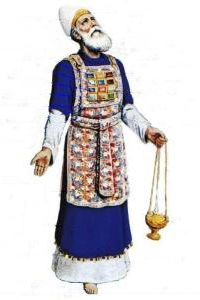
\includegraphics[width=50mm,scale=1.5]{Extras/Melchisedec.jpg}
\vspace{0.4in}  % Create a title for the document and write it in bold font
\LARGE{\textbf{\date}} % Again, do a line break
\linebreak 
% Create a subtitle \large{with Outlines, Statistics, Cross References, and Notes}
\vspace{0.5in}
\begin{flushleft}
\LARGE{Day \#100: Sunday, 10 April 2022  \\}\vspace{0.25in}
\LARGE{2 Samuel 22-24 Psalm 100 Proverb 10}
\end{flushleft}
\vspace{0.6in}
\bigskip

\normalsize{Xenia, Oh.\\}
\normalsize{created: \today}
\vspace{1.3in}

\end{flushright}
\end{titlepage}

\newpage 
\tableofcontents\hypertarget{TOC}{}
\listoffigures
\listoftables

\hyphenation{A-bim-e-lech bre-thren E-phra-im  Gib-e-o-nites Jer-u-sa-lem through-out Phil-i-stines The-o-phil-us Am-a-le-kites ven-geance Mesh-el-e-mi-ah onan-ism Phar-a-oh thoughts grev-ous-ness Hach-a-liah adul-ter-er Shad-rach}

%%%%%%%%%%%%%%%%% EXTRA COLORS
%%%%%%%%%%%%%%%%% EXTRA COLORS
%%%%%%%%%%%%%%%%% EXTRA COLORS
\definecolor{champagne}{rgb}{0.97,0.91,0.81}
\definecolor{bone}{rgb}{0.89,0.85,0.79}

\definecolor{ForestGreen}{rgb}{0.00,0.29,0.098}
\definecolor{GIVING}{cmyk}{1,0.0,0.72,.1}

\definecolor{MLPE}{cmyk}{1,1,0,.45}
\definecolor{SOCCER}{cmyk}{.77, 0, .42, .49}
\definecolor{PAYBILL}{cmyk}{0,0.83,0.76,0.07}
\definecolor{SERMON}{cmyk}{.14,.9,0,.30} % aka seance \href{http://www.flatuicolorpicker.com/purple-cmyk-color-model/}{seance}
\definecolor{BIBLE}{cmyk}{0,.17,.74,.17}
\definecolor{WORKBLUE}{cmyk}{1, .5, 0, .6}
\definecolor{myOrange}{cmyk}{0, .4, .98, .03}
\definecolor{myTan}{cmyk}{0.0,.07,.17,.10}
\definecolor{myRed}{cmyk}{0,1,1,0}
\definecolor{myWhite}{cmyk}{0,0,0,0}
\definecolor{BLUESoD}{cmyk}{.97,.84,0,.04}
\definecolor{WHITE}{cmyk}{0,0,0,0}
\definecolor{OLDGOLD}{cmyk}{0.05,0.3,1.00,0}
\definecolor{CASTLETON}{cmyk}{1,0,0.31,0.66}
\definecolor{cadmiumgreen}{rgb}{0.0, 0.42, 0.24}
\definecolor{jungle}{rgb}{0.203,0.4882,0.1718}
\definecolor{MYGOLD}{rgb}{1,.84,0}

\definecolor{MYLIGHTGRAY}{rgb}{.85,.85,.85}

\definecolor{codegreen}{rgb}{0,0.6,0}
\definecolor{codegray}{rgb}{0.5,0.5,0.5}
\definecolor{codepurple}{rgb}{0.58,0,0.82}
\definecolor{backcolour}{rgb}{0.95,0.95,0.92}


\mdfdefinestyle{MyFrame}{%
    linecolor=blue,
    outerlinewidth=2pt,
    roundcorner=5pt,
    innertopmargin=\baselineskip,
    innerbottommargin=\baselineskip,
    innerrightmargin=10pt,
    innerleftmargin=10pt,
    backgroundcolor=gray!25!white}


\mdfdefinestyle{MyFrame2}{%
    linecolor=black,
    outerlinewidth=2pt,
    roundcorner=5pt,
    innertopmargin=\baselineskip,
    innerbottommargin=\baselineskip,
    innerrightmargin=10pt,
    innerleftmargin=10pt,
    backgroundcolor=yellow!25!white}


%%%%%
%% for PFTTIS list
%%%%%

%%% And Joseph said unto
\index[PFTTIS]{And Joseph said unto!Genesis!Gen 40:008}
\index[PFTTIS]{And Joseph said unto!Genesis!Gen 40:012}
\index[PFTTIS]{And Joseph said unto!Genesis!Gen 41:025}
\index[PFTTIS]{And Joseph said unto!Genesis!Gen 42:014}
\index[PFTTIS]{And Joseph said unto!Genesis!Gen 42:018}
\index[PFTTIS]{And Joseph said unto!Genesis!Gen 44:015}
\index[PFTTIS]{And Joseph said unto!Genesis!Gen 45:003}
\index[PFTTIS]{And Joseph said unto!Genesis!Gen 45:004}
\index[PFTTIS]{And Joseph said unto!Genesis!Gen 46:031}
\index[PFTTIS]{And Joseph said unto!Genesis!Gen 48:009}
\index[PFTTIS]{And Joseph said unto!Genesis!Gen 48:018}
\index[PFTTIS]{And Joseph said unto!Genesis!Gen 50:019}
\index[PFTTIS]{And Joseph said unto!Genesis!Gen 50:024}


%%% a shadow
\index[PFTTIS]{a shadow!1Chronicles!1Chr 029:15}
\index[PFTTIS]{a shadow!Job!Job 008:09}
\index[PFTTIS]{a shadow!Job!Job 014:02}
\index[PFTTIS]{a shadow!Job!Job 017:07}
\index[PFTTIS]{a shadow!Psalm!Psa 102:011}
\index[PFTTIS]{a shadow!Psalm!Psa 144:004}
\index[PFTTIS]{a shadow!Ecclesiastes!Eccl 006:012}
\index[PFTTIS]{a shadow!Ecclesiastes!Eccl 008:013}
\index[PFTTIS]{a shadow!Isaiah!Isa 04:006}
\index[PFTTIS]{a shadow!Isaiah!Isa 25:004}
\index[PFTTIS]{a shadow!Jonah!Jnh 04:06}
\index[PFTTIS]{a shadow!Colossians!Col 02:017}
\index[PFTTIS]{a shadow!Hebews!Heb 10:001}

%%% blessed is the man
\index[PFTTIS]{blessed is the man!Psalm!Psa 001:001}
\index[PFTTIS]{blessed is the man!Psalm!Psa 032:002}
\index[PFTTIS]{blessed is the man!Psalm!Psa 034:008}
\index[PFTTIS]{blessed is the man!Psalm!Psa 065:004}
\index[PFTTIS]{blessed is the man!Psalm!Psa 084:005}
\index[PFTTIS]{blessed is the man!Psalm!Psa 084:012}
\index[PFTTIS]{blessed is the man!Psalm!Psa 094:012}
\index[PFTTIS]{blessed is the man!Psalm!Psa 112:001}
\index[PFTTIS]{blessed is the man!Proverbs!Pro 008:034}
\index[PFTTIS]{blessed is the man!Isaiah!Isa 056:002}
\index[PFTTIS]{blessed is the man!Jeremiah!Jer 017:007}
\index[PFTTIS]{blessed is the man!Romans!Rom 004:008}
\index[PFTTIS]{blessed is the man!James!Jam 001:012}


%%% carry them
\index[PFTTIS]{carry them!Leviticus!Lev 14:045}
\index[PFTTIS]{carry them!Numbers!Num 11:012}
\index[PFTTIS]{carry them!Joshua!Jsh 04:003}
\index[PFTTIS]{carry them!1Samuel!1Sam 20:040}
\index[PFTTIS]{carry them!1Kings!1Kng 08:046}
\index[PFTTIS]{carry them!2Chronicles!2Chr 06:036}
\index[PFTTIS]{carry them!Ezra!Ezra 05:015}
\index[PFTTIS]{carry them!Isaiah!Isa 40:011}
\index[PFTTIS]{carry them!Isaiah!Isa 41:016}
\index[PFTTIS]{carry them!Isaiah!Isa 57:013}
\index[PFTTIS]{carry them!Jeremiah!Jer 20:004}
\index[PFTTIS]{carry them!Jeremiah!Jer 20:005}
\index[PFTTIS]{carry them!Jeremiah!Jer 43:012}


\index[PFTTIS]{good tidings!2Samuel!2Sam 18:027}
\index[PFTTIS]{good tidings!1Kings!1Ki 01:042}
\index[PFTTIS]{good tidings!2Kings!2Ki 07:009 (2x)}
\index[PFTTIS]{good tidings!Isaiah!Isa 40:009 (2x)}
\index[PFTTIS]{good tidings!Isaiah!Isa 41:007}
\index[PFTTIS]{good tidings!Isaiah!Isa 52:007}
\index[PFTTIS]{good tidings!Isaiah!Isa 61:001}
\index[PFTTIS]{good tidings!Nahum!Nah 01:005}
\index[PFTTIS]{good tidings!Luke!Lk 02:010}
\index[PFTTIS]{good tidings!1Thessalonians!1Thess 03:006}


%%% dead body
\index[PFTTIS]{dead body!Leviticus!Lev 21:011}
\index[PFTTIS]{dead body!Numbers!Num 06:006}
\index[PFTTIS]{dead body!Numbers!Num 09:006}
\index[PFTTIS]{dead body!Numbers!Num 09:007}
\index[PFTTIS]{dead body!Numbers!Num 09:010}
\index[PFTTIS]{dead body!Numbers!Num 09:011}
\index[PFTTIS]{dead body!Numbers!Num 09:013}
\index[PFTTIS]{dead body!Numbers!Num 09:016}
\index[PFTTIS]{dead body!2Kings!2Ki 08:005}
\index[PFTTIS]{dead body!Isaiah!Isa 26:019}
\index[PFTTIS]{dead body!Jeremiah!Jer 26:023}
\index[PFTTIS]{dead body!Jeremiah!Jer 36:030}
\index[PFTTIS]{dead body!Haggai!Hag 02:013}

%%% great sea
\index[PFTTIS]{great sea!Numbers!Num 34:006}
\index[PFTTIS]{great sea!Numbers!Num 34:007}
\index[PFTTIS]{great sea!Joshua!Jos 01:004}
\index[PFTTIS]{great sea!Joshua!Jos 09:001}
\index[PFTTIS]{great sea!Joshua!Jos 15:012}
\index[PFTTIS]{great sea!Joshua!Jos 15:047}
\index[PFTTIS]{great sea!Joshua!Jos 23:004}
\index[PFTTIS]{great sea!Ezekiel!Eze 47:010}
\index[PFTTIS]{great sea!Ezekiel!Eze 47:015}
\index[PFTTIS]{great sea!Ezekiel!Eze 47:019}
\index[PFTTIS]{great sea!Ezekiel!Eze 47:020}
\index[PFTTIS]{great sea!Ezekiel!Eze 48:028}
\index[PFTTIS]{great sea!Daniel!Dan 07:002}


%%% have forsaken me
\index[PFTTIS]{have forsaken me!Judges!Jdg 10:013}
\index[PFTTIS]{have forsaken me!1Samuel!1Sam 08:008}
\index[PFTTIS]{have forsaken me!1Kings!1Ki 11:033}
\index[PFTTIS]{have forsaken me!2Kings!2Ki 22:017}
\index[PFTTIS]{have forsaken me!2Chronicles!2Chr 12:005}
\index[PFTTIS]{have forsaken me!2Chronicles!2Chr 34:025}
\index[PFTTIS]{have forsaken me!Jeremiah!Jer 01:016}
\index[PFTTIS]{have forsaken me!Jeremiah!Jer 02:013}
\index[PFTTIS]{have forsaken me!Jeremiah!Jer 05:007}
\index[PFTTIS]{have forsaken me!Jeremiah!Jer 05:019}
\index[PFTTIS]{have forsaken me!Jeremiah!Jer 16:011 (2x)}
\index[PFTTIS]{have forsaken me!Jeremiah!Jer 19:004}

%%% no king
\index[PFTTIS]{no king!Judges!Jdg 17:06}
\index[PFTTIS]{no king!Judges!Jdg 18:01}
\index[PFTTIS]{no king!Judges!Jdg 19:01}
\index[PFTTIS]{no king!Judges!Jdg 21:25}
\index[PFTTIS]{no king!1Kings!1Ki 22:47}
\index[PFTTIS]{no king!2Kings!2Ki 23:25}
\index[PFTTIS]{no king!Nehemiah!Neh 13:26}
\index[PFTTIS]{no king!Psalms!Psa 033:016}
\index[PFTTIS]{no king!Proverbs!Pro 30:27}
\index[PFTTIS]{no king!Daniel!Dan 02:10}
\index[PFTTIS]{no king!Hosea!Hos 10:03}
\index[PFTTIS]{no king!Micah!Mic 04:09}
\index[PFTTIS]{no king!John!Jhn 19:15}


%%% rebellious house
\index[PFTTIS]{rebellious house!Exodus!Exo 02:005}
\index[PFTTIS]{rebellious house!Exodus!Exo 02:006}
\index[PFTTIS]{rebellious house!Exodus!Exo 02:008}
\index[PFTTIS]{rebellious house!Exodus!Exo 03:009}
\index[PFTTIS]{rebellious house!Exodus!Exo 03:026}
\index[PFTTIS]{rebellious house!Exodus!Exo 03:027}
\index[PFTTIS]{rebellious house!Exodus!Exo 12:002 (2x)}
\index[PFTTIS]{rebellious house!Exodus!Exo 12:003}
\index[PFTTIS]{rebellious house!Exodus!Exo 12:009}
\index[PFTTIS]{rebellious house!Exodus!Exo 12:025}
\index[PFTTIS]{rebellious house!Exodus!Exo 17:012}
\index[PFTTIS]{rebellious house!Exodus!Exo 24:003}

%%% seek him
\index[PFTTIS]{seek him!Deuteronomy!Deu 04:029}\index[PFTTIS]{seek him!1Samuel!1Sam 23:025}
\index[PFTTIS]{seek him!1Chronicles!1Chr 28:009}
\index[PFTTIS]{seek him!2Chronicles!1Chr 15:002}
\index[PFTTIS]{seek him!Ezra!Ezr 08:022}
\index[PFTTIS]{seek him!Psalms!Psa 022:026}
\index[PFTTIS]{seek him!Psalms!Psa 024:006}
\index[PFTTIS]{seek him!Psalms!Psa 119:002}
\index[PFTTIS]{seek him!SoS!SoS 03:002}
\index[PFTTIS]{seek him!SoS!SoS 06:001}
\index[PFTTIS]{seek him!Hosea!Hos 07:010}
\index[PFTTIS]{seek him!Amos!Amo 05:008}
\index[PFTTIS]{seek him!Hebrews!Heb 11:0063}


%%% seek ye
\index[PFTTIS]{seek ye!Isaiah!Isa 34:016}
\index[PFTTIS]{seek ye!Isaiah!Isa 45:019}
\index[PFTTIS]{seek ye!Isaiah!Isa 55:006}
\index[PFTTIS]{seek ye!Amos!Amos 5:004}
\index[PFTTIS]{seek ye!John!John 1:38}
\index[PFTTIS]{seek ye!John!John 18:4}
\index[PFTTIS]{seek ye!John!John 18:7}
\index[PFTTIS]{seek ye!Matthew!Matt 6:33}
\index[PFTTIS]{seek ye!Numbers!Num 16:10}
\index[PFTTIS]{seek ye!Luke!Luke 12:31}
\index[PFTTIS]{seek ye!Luke!Luke 24:5}
\index[PFTTIS]{seek ye!Psalm!Psa 27:8}
\index[PFTTIS]{seek ye!Zephaniah!Zeph 2:3}

%%% the uncircumcised
\index[PFTTIS]{the uncircumcised!Genesis!Gen 17:014}
\index[PFTTIS]{the uncircumcised!Judges!Jdg 14:003}
\index[PFTTIS]{the uncircumcised!Judges!Jdg 15:018}
\index[PFTTIS]{the uncircumcised!2Samuel!2Sam 01:020}
\index[PFTTIS]{the uncircumcised!Isaiah!Isa 02:001}
\index[PFTTIS]{the uncircumcised!Jeremiah!Jer 09:025}
\index[PFTTIS]{the uncircumcised!Ezekiel!Eze 28:010}
\index[PFTTIS]{the uncircumcised!Ezekiel!Eze 31:018}
\index[PFTTIS]{the uncircumcised!Ezekiel!Eze 32:019}
\index[PFTTIS]{the uncircumcised!Ezekiel!Eze 32:027}
\index[PFTTIS]{the uncircumcised!Ezekiel!Eze 32:028}
\index[PFTTIS]{the uncircumcised!Ezekiel!Eze 32:029}
\index[PFTTIS]{the uncircumcised!Ezekiel!Eze 32:032}

%%% worship him
\index[PFTTIS]{worship him!Psalms!Psa 97:007}
\index[PFTTIS]{worship him!Zephaniah!Zeph 02:011}
\index[PFTTIS]{worship him!Matthew!Matt 02:002}
\index[PFTTIS]{worship him!Matthew!Matt 02:008}
\index[PFTTIS]{worship him!John!John 04:023}
\index[PFTTIS]{worship him!John!John 04:024 (2x)} 
\index[PFTTIS]{worship him!Acts!Acts 17:023}
\index[PFTTIS]{worship him!Hebrews!Heb 01:006}
\index[PFTTIS]{worship him!Revelation!Rev 04:010}
\index[PFTTIS]{worship him!Revelation!Rev 13:008}
\index[PFTTIS]{worship him!Revelation!Rev 14:007}
\index[PFTTIS]{worship him!Revelation!Rev 19:010}


%%%%%
%% for PFTTIS list
%%%%%

%%% afflictions
\index[WFTTIS]{afflictions!Psalms!Psa 34:019}
\index[WFTTIS]{afflictions!Psalms!Psa 132:001}
\index[WFTTIS]{afflictions!Acts!Acts 07:010}
\index[WFTTIS]{afflictions!Acts!Acts 20:023}
\index[WFTTIS]{afflictions!2Corinthians!2Cor 06:004}
\index[WFTTIS]{afflictions!Colossians!Col 01:024}
\index[WFTTIS]{afflictions!1Thessalonians!1Thess 03:003}
\index[WFTTIS]{afflictions!2Timothy!2Tim 01:008}
\index[WFTTIS]{afflictions!2Timothy!2Tim 03:011}
\index[WFTTIS]{afflictions!2Timothy!2Tim 04:005}
\index[WFTTIS]{afflictions!Hebrews!Heb 10:032}
\index[WFTTIS]{afflictions!Hebrews!Heb 10:033}
\index[WFTTIS]{afflictions!1Peter!1Pet 05:009}

%%% acsend
\index[WFTTIS]{acsend!Joshua!Jos 06:05}
\index[WFTTIS]{acsend!Psalm!Psa 024:003}
\index[WFTTIS]{acsend!Psalm!Psa 135:007}
\index[WFTTIS]{acsend!Psalm!Psa 139:008}
\index[WFTTIS]{acsend!Isaiah!Isa 14:013}
\index[WFTTIS]{acsend!Isaiah!Isa 14:014}
\index[WFTTIS]{acsend!Jeremiah!Jer 10:013}
\index[WFTTIS]{acsend!Jeremiah!Jer 51:016}
\index[WFTTIS]{acsend!Ezekiel!Eze 38:009}
\index[WFTTIS]{acsend!John!John 06:062}
\index[WFTTIS]{acsend!John!John 20:017}
\index[WFTTIS]{acsend!Romans!Rom 10:006}
\index[WFTTIS]{acsend!Revelation!Rev 17:008}

%%% Assyrian
\index[WFTTIS]{Assyrian!Isaiah!Isa 10:005}
\index[WFTTIS]{Assyrian!Isaiah!Isa 10:024}
\index[WFTTIS]{Assyrian!Isaiah!Isa 14:025}
\index[WFTTIS]{Assyrian!Isaiah!Isa 19:023}
\index[WFTTIS]{Assyrian!Isaiah!Isa 23:013}
\index[WFTTIS]{Assyrian!Isaiah!Isa 30:031}
\index[WFTTIS]{Assyrian!Isaiah!Isa 31:008}
\index[WFTTIS]{Assyrian!Isaiah!Isa 52:004}
\index[WFTTIS]{Assyrian!Ezekiel!Eze 31:003}
\index[WFTTIS]{Assyrian!Hosea!Hos 05:013}
\index[WFTTIS]{Assyrian!Hosea!Hos 11:005}
\index[WFTTIS]{Assyrian!Micah!Hos 05:005}
\index[WFTTIS]{Assyrian!Micah!Hos 05:006}

%%% blot
\index[WFTTIS]{blot!Exodus!Exo 32:032}
\index[WFTTIS]{blot!Exodus!Exo 32:033}
\index[WFTTIS]{blot!Numbers!Num 05:026}
\index[WFTTIS]{blot!Deuteronomy!Deut 09:014}
\index[WFTTIS]{blot!Deuteronomy!Deut 25:019}
\index[WFTTIS]{blot!Deuteronomy!Deut 29:020}
\index[WFTTIS]{blot!2Kings!2Ki 14:027}
\index[WFTTIS]{blot!Job!Job 31:007}
\index[WFTTIS]{blot!Psalms!Psa 51:001}
\index[WFTTIS]{blot!Psalms!Psa 51:009}
\index[WFTTIS]{blot!Proverbs!Pro 09:007}
\index[WFTTIS]{blot!Jeremiah!Jer 18:023}
\index[WFTTIS]{blot!Revelation!Rev 03:005}


%%% chain
\index[WFTTIS]{chain!Genesis!Gen 41:042}
\index[WFTTIS]{chain!1Kings!1Ki 07:017}
\index[WFTTIS]{chain!Psalms!Psa 73:006}
\index[WFTTIS]{chain!SoS!Sos 04:009}
\index[WFTTIS]{chain!Lamentations!Lam 03:007}
\index[WFTTIS]{chain!Ezekiel!Eze 07:023}
\index[WFTTIS]{chain!Ezekiel!Eze 16:011}
\index[WFTTIS]{chain!Daniel!Dan 05:007}
\index[WFTTIS]{chain!Daniel!Dan 05:016}
\index[WFTTIS]{chain!Daniel!Dan 05:029}
\index[WFTTIS]{chain!Acts!Acts 28:020}
\index[WFTTIS]{chain!2Timothy!2Tim 01:016}
\index[WFTTIS]{chain!Revelation!Rev 20:001}


%%% controversy
\index[WFTTIS]{controversy!Deuteronomy!Deu 17:008}
\index[WFTTIS]{controversy!Deuteronomy!Deu 19:017}
\index[WFTTIS]{controversy!Deuteronomy!Deu 21:005}
\index[WFTTIS]{controversy!Deuteronomy!Deu 25:001}
\index[WFTTIS]{controversy!2Samuel!2Sam 15:002}
\index[WFTTIS]{controversy!Isaiah!Isa 34:008}
\index[WFTTIS]{controversy!Jeremiah!Jer 25:031}
\index[WFTTIS]{controversy!Ezekiel!Eze 44:024}
\index[WFTTIS]{controversy!Hosea!Hos 04:001}
\index[WFTTIS]{controversy!Hosea!Hos 12:002}
\index[WFTTIS]{controversy!Micah!Mic 06:002 (2x)}
\index[WFTTIS]{controversy!1Timothy!1Tim 03:016}


%%% Dagon/Dagon's
\index[WFTTIS]{Dagon!Judges!Jdg 16:023}
\index[WFTTIS]{Dagon!1Samuel!1Sam 05:002 (2x)}
\index[WFTTIS]{Dagon!1Samuel!1Sam 05:003 (2x)}
\index[WFTTIS]{Dagon!1Samuel!1Sam 05:004 (3x)}
\index[WFTTIS]{Dagon!1Samuel!1Sam 05:005 (3x)}
\index[WFTTIS]{Dagon!1Samuel!1Sam 05:007}
\index[WFTTIS]{Dagon!1Chronicles!1Chr 10:010}

%%% disobedient
\index[WFTTIS]{disobedient!1Kings!1Ki 13:026}
\index[WFTTIS]{disobedient!Nehemiah!Neh 09:026}
\index[WFTTIS]{disobedient!Luke!Luke 01:017}
\index[WFTTIS]{disobedient!Acts!Acts 26:019}
\index[WFTTIS]{disobedient!Romans!Rom 01:030}
\index[WFTTIS]{disobedient!Romans!Rom 10:021}
\index[WFTTIS]{disobedient!1Timothy!1Tim 01:009}
\index[WFTTIS]{disobedient!2Timothy!2Tim 03:002}
\index[WFTTIS]{disobedient!Titus!Titus 01:016}
\index[WFTTIS]{disobedient!Titus!Titus 03:003}
\index[WFTTIS]{disobedient!1Peter!1Pet 02:007}
\index[WFTTIS]{disobedient!1Peter!1Pet 02:008}
\index[WFTTIS]{disobedient!1Peter!1Pet 03:020}


%%% doubt
\index[WFTTIS]{doubt!Genesis!Gen 37:033}
\index[WFTTIS]{doubt!Deuteronomy!Deu 28:066}
\index[WFTTIS]{doubt!Job!Job 12:002}
\index[WFTTIS]{doubt!Matthew!Matt 14:031}
\index[WFTTIS]{doubt!Matthew!Matt 21:021}
\index[WFTTIS]{doubt!Mark!Mk 11:023}
\index[WFTTIS]{doubt!Luke!Lk 11:020}
\index[WFTTIS]{doubt!John!Jhn 10:024}
\index[WFTTIS]{doubt!Acts!Acts 02:012}
\index[WFTTIS]{doubt!Acts!Acts 28:004}
\index[WFTTIS]{doubt!1Corinthians!1Cor 09:010}
\index[WFTTIS]{doubt!Galatians!Gal 04:020}
\index[WFTTIS]{doubt!1John!1Jhn 02:019}


%%% dungeon
\index[WFTTIS]{dungeon!Genesis!Gen 40:015}
\index[WFTTIS]{dungeon!Genesis!Gen 41:014}
\index[WFTTIS]{dungeon!Exodus!Exo 12:029}
\index[WFTTIS]{dungeon!Jeremiah!Jer 37:016}
\index[WFTTIS]{dungeon!Jeremiah!Jer 38:006 (2x)}
\index[WFTTIS]{dungeon!Jeremiah!Jer 38:007}
\index[WFTTIS]{dungeon!Jeremiah!Jer 38:009}
\index[WFTTIS]{dungeon!Jeremiah!Jer 38:010}
\index[WFTTIS]{dungeon!Jeremiah!Jer 38:011}
\index[WFTTIS]{dungeon!Jeremiah!Jer 38:013}
\index[WFTTIS]{dungeon!Lamentations!Lam 03:053}
\index[WFTTIS]{dungeon!Lamentations!Lam 03:055}


%%% error
\index[WFTTIS]{error!2Samuel!2Sam 06:007}
\index[WFTTIS]{error!Job!Job 19:004}
\index[WFTTIS]{error!Ecclesiastes!Ecc 05:006}
\index[WFTTIS]{error!Ecclesiastes!Ecc 10:005}
\index[WFTTIS]{error!Isaiah!Isa 32:006}
\index[WFTTIS]{error!Daniel!Dan 06:004}
\index[WFTTIS]{error!Matthew!Matt 27:064}
\index[WFTTIS]{error!Romans!Rom 01:027}
\index[WFTTIS]{error!James!Jam 05:020}
\index[WFTTIS]{error!2Peter!2Pet 02:018}
\index[WFTTIS]{error!2Peter!2Pet 03:017}
\index[WFTTIS]{error!1John!1Jn 04:006}
\index[WFTTIS]{error!Jude!Jude 01:011}

%%% fourish
\index[WFTTIS]{fourish!Psalms!Psa 072:007}
\index[WFTTIS]{fourish!Psalms!Psa 072:016}
\index[WFTTIS]{fourish!Psalms!Psa 092:007}
\index[WFTTIS]{fourish!Psalms!Psa 092:012}
\index[WFTTIS]{fourish!Psalms!Psa 092:013}
\index[WFTTIS]{fourish!Psalms!Psa 132:018}
\index[WFTTIS]{fourish!Proverbs!Pro 11:28}
\index[WFTTIS]{fourish!Proverbs!Pro 14:11}
\index[WFTTIS]{fourish!Ecclesiastes!Ecc 12:05}
\index[WFTTIS]{fourish!SongOfSolomon!SOS 07:12}
\index[WFTTIS]{fourish!Isaiah!Isa 17:11}
\index[WFTTIS]{fourish!Isaiah!Isa 66:14}
\index[WFTTIS]{fourish!Ezekiel!Eze 17:24}




%%% giants
\index[WFTTIS]{giants!Genesis!Gen 06:004}
\index[WFTTIS]{giants!Numbers!Num 13:033}
\index[WFTTIS]{giants!Deuteronomy!Deut 02:011}
\index[WFTTIS]{giants!Deuteronomy!Deut 02:021}
\index[WFTTIS]{giants!Deuteronomy!Deut 03:011}
\index[WFTTIS]{giants!Deuteronomy!Deut 03:013}
\index[WFTTIS]{giants!Joshua!Josh 12:004}
\index[WFTTIS]{giants!Joshua!Josh 13:012}
\index[WFTTIS]{giants!Joshua!Josh 15:008}
\index[WFTTIS]{giants!Joshua!Josh 17:015}
\index[WFTTIS]{giants!Joshua!Josh 16:016}

%%% good man
\index[WFTTIS]{good man!2 Samuel!2Sa 18:27}
%(1) Psalms 37:23 [5]
%(1) Psalms 112:5 [2]
%(1) Proverbs 12:2 [2]
%(1) Proverbs 13:22 [2]
%(1) Proverbs 14:14 [14]
%(1) Micah 7:2 [2]
%(1) Matthew 12:35 [2]
%(1) Luke 6:45 [2]
%(1) Luke 23:50 [15]
%(1) John 7:12 [17]
%(1) Acts 11:24 [5]
%(1) Romans 5:7 [14]

%%% Hinnom
\index[WFTTIS]{Hinnom!Joshua!Jsh 15:008}
\index[WFTTIS]{Hinnom!Joshua!Jsh 18:016}
\index[WFTTIS]{Hinnom!2Kings!2Ki 23:010}
\index[WFTTIS]{Hinnom!2Chronicles!2Chr 28:003}
\index[WFTTIS]{Hinnom!2Chronicles!2Chr 33:006}
\index[WFTTIS]{Hinnom!Nehemiah!Neh 11:030}
\index[WFTTIS]{Hinnom!Jeremiah!Jer 07:031}
\index[WFTTIS]{Hinnom!Jeremiah!Jer 07:032}
\index[WFTTIS]{Hinnom!Jeremiah!Jer 19:002}
\index[WFTTIS]{Hinnom!Jeremiah!Jer 19:006}
\index[WFTTIS]{Hinnom!Jeremiah!Jer 32:035}

%%% inclined
\index[WFTTIS]{inclined!Judges!Jdg 09:003}
\index[WFTTIS]{inclined!Psalms!Psa 040:001}
\index[WFTTIS]{inclined!Psalms!Psa 116:002}
\index[WFTTIS]{inclined!Psalms!Psa 119:112}
\index[WFTTIS]{inclined!Proverbs!Pro 05:13}
\index[WFTTIS]{inclined!Jeremiah!Jer 07:24}
\index[WFTTIS]{inclined!Jeremiah!Jer 07:26}
\index[WFTTIS]{inclined!Jeremiah!Jer 11:08}
\index[WFTTIS]{inclined!Jeremiah!Jer 17:23}
\index[WFTTIS]{inclined!Jeremiah!Jer 25:04}
\index[WFTTIS]{inclined!Jeremiah!Jer 34:14}
\index[WFTTIS]{inclined!Jeremiah!Jer 35:15}
\index[WFTTIS]{inclined!Jeremiah!Jer 44:05}


%%% laughed
\index[WFTTIS]{laughed!Genesis!Gen 17:017}
\index[WFTTIS]{laughed!Genesis!Gen 18:012}
\index[WFTTIS]{laughed!Genesis!Gen 18:015}
\index[WFTTIS]{laughed!2Kings!2Ki 19:021}
\index[WFTTIS]{laughed!2Chronicles!2Chr 30:010}
\index[WFTTIS]{laughed!Nehemiah!Neh 02:019}
\index[WFTTIS]{laughed!Job!Job 12:004}
\index[WFTTIS]{laughed!Job!Job 29:024}
\index[WFTTIS]{laughed!Isaiah!Isa 37:022}
\index[WFTTIS]{laughed!Ezekiel!Ezek 23:032}
\index[WFTTIS]{laughed!Matthew!Matt 09:024}
\index[WFTTIS]{laughed!Mark!Mk 05:040}
\index[WFTTIS]{laughed!Luke!Lk 08:053}

%%% liar
\index[WFTTIS]{liar!Job!Job 24:025}
\index[WFTTIS]{liar!Proverbs!Pro 17:004}
\index[WFTTIS]{liar!Proverbs!Pro 19:022}
\index[WFTTIS]{liar!Proverbs!Pro 30:006}
\index[WFTTIS]{liar!Jeremiah!Jer 15:018}
\index[WFTTIS]{liar!John!Jhn 08:044}
\index[WFTTIS]{liar!John!Jhn 08:055}
\index[WFTTIS]{liar!Romans!Rom 03:004}
\index[WFTTIS]{liar!1John!1Jhn 01:010}
\index[WFTTIS]{liar!1John!1Jhn 02:004}
\index[WFTTIS]{liar!1John!1Jhn 02:022}
\index[WFTTIS]{liar!1John!1Jhn 04:020}
\index[WFTTIS]{liar!1John!1Jhn 05:010}

%%% palsy
\index[WFTTIS]{palsy!Matthew!Matt 04:024}
\index[WFTTIS]{palsy!Matthew!Matt 08:006}
\index[WFTTIS]{palsy!Matthew!Matt 09:002}
\index[WFTTIS]{palsy!Matthew!Matt 09:006}
\index[WFTTIS]{palsy!Mark!Mk 02:003}
\index[WFTTIS]{palsy!Mark!Mk 02:004}
\index[WFTTIS]{palsy!Mark!Mk 02:005}
\index[WFTTIS]{palsy!Mark!Mk 02:009}
\index[WFTTIS]{palsy!Mark!Mk 02:010}
\index[WFTTIS]{palsy!Luke!Lk 05:018}
\index[WFTTIS]{palsy!Luke!Lk 05:024}
\index[WFTTIS]{palsy!Acts!Acts 09:033}

%%% Profitable
\index[WFTTIS]{profitable!Job!Job 22:002 (2x)}
\index[WFTTIS]{profitable!Ecclesiastes!Ecc 10:010}
\index[WFTTIS]{profitable!Isaiah!Isa 44:010}
\index[WFTTIS]{profitable!Jeremiah!Jer 13:007}
\index[WFTTIS]{profitable!Matthew!Matt 05:029}
\index[WFTTIS]{profitable!Matthew!Matt 05:030}
\index[WFTTIS]{profitable!Acts!Acts 20:020}
\index[WFTTIS]{profitable!1Timothy!1Tim 04:008}
\index[WFTTIS]{profitable!2Timothy!2Tim 03:016}
\index[WFTTIS]{profitable!2Timothy!2Tim 04:011}
\index[WFTTIS]{profitable!Titus!Titus 03:008}
\index[WFTTIS]{profitable!Philemon!Phlm 01:011}

%%% Rechab
\index[WFTTIS]{Rechab!2Samuel!2Sam 04:002}
\index[WFTTIS]{Rechab!2Samuel!2Sam 04:005}
\index[WFTTIS]{Rechab!2Samuel!2Sam 04:006}
\index[WFTTIS]{Rechab!2Samuel!2Sam 04:009}
\index[WFTTIS]{Rechab!2KIngs!2Ki 10:015}
\index[WFTTIS]{Rechab!2KIngs!2Ki 10:023}
\index[WFTTIS]{Rechab!1Chronicles!1Chr 02:055}
\index[WFTTIS]{Rechab!Nehemiah!Neh 03:014}
\index[WFTTIS]{Rechab!Jeremiah!Jer 35:006}
\index[WFTTIS]{Rechab!Jeremiah!Jer 35:008}
\index[WFTTIS]{Rechab!Jeremiah!Jer 35:014}
\index[WFTTIS]{Rechab!Jeremiah!Jer 35:016}
\index[WFTTIS]{Rechab!Jeremiah!Jer 35:019}

%%% serpents
\index[WFTTIS]{serpents!Exodus!Exo 07:012}
\index[WFTTIS]{serpents!Numbers!Num 21:006}
\index[WFTTIS]{serpents!Numbers!Num 21:007}
\index[WFTTIS]{serpents!Deuteronomy!Deu 08:015}
\index[WFTTIS]{serpents!Deuteronomy!Deu 32:024}
\index[WFTTIS]{serpents!Jeremiah!Jer 08:017}
\index[WFTTIS]{serpents!Matthew!Matt 10:016}
\index[WFTTIS]{serpents!Matthew!Matt 23:033}
\index[WFTTIS]{serpents!Mark!Mk 16:018}
\index[WFTTIS]{serpents!Luke!Lk 10:019}
\index[WFTTIS]{serpents!1Corinthians!1Cor 10:009}
\index[WFTTIS]{serpents!James!Jas 03:007}
\index[WFTTIS]{serpents!Revelation!Rev 09:019}

%%% short
\index[WFTTIS]{short!Numbers!Num 11:023}
\index[WFTTIS]{short!2Kings!2Ki 10:032}
\index[WFTTIS]{short!Job!Job 17:012}
\index[WFTTIS]{short!Job!Job 20:005}
\index[WFTTIS]{short!Psalms!Psa 89:047}
\index[WFTTIS]{short!Romans!Rom 03:023}
\index[WFTTIS]{short!Romans!Rom 09:028  (2x)}
\index[WFTTIS]{short!1Corinthians!1Cor 07:029}
\index[WFTTIS]{short!1Thessalonians!1Thess 02:017}
\index[WFTTIS]{short!Hebrews!Heb 04:001}
\index[WFTTIS]{short!Revelation!Rev 12:012}
\index[WFTTIS]{short!Revelation!Rev 17:010}

%%% smiteth
\index[WFTTIS]{smiteth!Exodus!Exo 21:012}
\index[WFTTIS]{smiteth!Exodus!Exo 21:15}
\index[WFTTIS]{smiteth!Deuteronomy!Dt 25:11}
\index[WFTTIS]{smiteth!Deuteronomy!Dt 27:24}
\index[WFTTIS]{smiteth!Joshua!Jsh 15:16}
\index[WFTTIS]{smiteth!Judges!Jdg 15:16}
\index[WFTTIS]{smiteth!2 Samuel!2Sa 05:08}
\index[WFTTIS]{smiteth!1Chronicles!1Chr 11:06}
\index[WFTTIS]{smiteth!Job!1Chr 26:12}
\index[WFTTIS]{smiteth!Isaiah!Isa 09:13}
\index[WFTTIS]{smiteth!Lamentations!Lam 03:30}
\index[WFTTIS]{smiteth!Ezekiel!Eze 07:09}
\index[WFTTIS]{smiteth!Luke!Lk 06:29}



%%% vanities
\index[WFTTIS]{vanities!Deuteronomy!Deut 21:021}
\index[WFTTIS]{vanities!1Kings!1Ki 16:013}
\index[WFTTIS]{vanities!1Kings!1Ki 16:026}
\index[WFTTIS]{vanities!Psalms!Psa 031:006}
\index[WFTTIS]{vanities!Ecclesiastes!Ecc 01:002 (2x)}
\index[WFTTIS]{vanities!Ecclesiastes!Ecc 05:007}
\index[WFTTIS]{vanities!Ecclesiastes!Ecc 12:008}
\index[WFTTIS]{vanities!Jeremiah!Jer 08:019}
\index[WFTTIS]{vanities!Jeremiah!Jer 10:008}
\index[WFTTIS]{vanities!Jeremiah!Jer 14:022}
\index[WFTTIS]{vanities!Jonah!Jnh 02:008}
\index[WFTTIS]{vanities!Acts!Acts 14:015}



%%%%%
%% for PFTTIS list
%%%%%

%%% worm
\index[WFITV]{worm!Exodus!Exo 16:024}
\index[WFITV]{worm!Job!Job 17:014}
\index[WFITV]{worm!Job!Job 24:029}
\index[WFITV]{worm!Job!Job 25:005 (2x)}
\index[WFITV]{worm!Psalms!Psa 022:006}
\index[WFITV]{worm!Isaiah!Isa 14:011}
\index[WFITV]{worm!Isaiah!Isa 41:014}
\index[WFITV]{worm!Isaiah!Isa 51:008}
\index[WFITV]{worm!Isaiah!Isa 66:024}
\index[WFITV]{worm!Jonah!Jnh 04:007}
\index[WFITV]{worm!Mark!Mk 09:044}
\index[WFITV]{worm!Mark!Mk 09:046}
\index[WFITV]{worm!Mark!Mk 09:048}


%\subsubsection{Title}
%\textbf{Introduction:} Isaiah 46 
%\index[speaker]{Speaker!Isaiah 49 (Title}
%\index[series]{Book (Speaker)!IPassage (Title)}
%\index[date]{2017/07/09!Isaiah 49 (Title)}
%\begin{compactenum}[I.]
%    \item  \textbf{Point} \index[scripture]{Isaiah!IPassage} (IPassage)
%\end{compactenum}




  


%\input{02OT-Exodus/ExodusIntroduction}

\newpage
\begin{figure}
\begin{center}
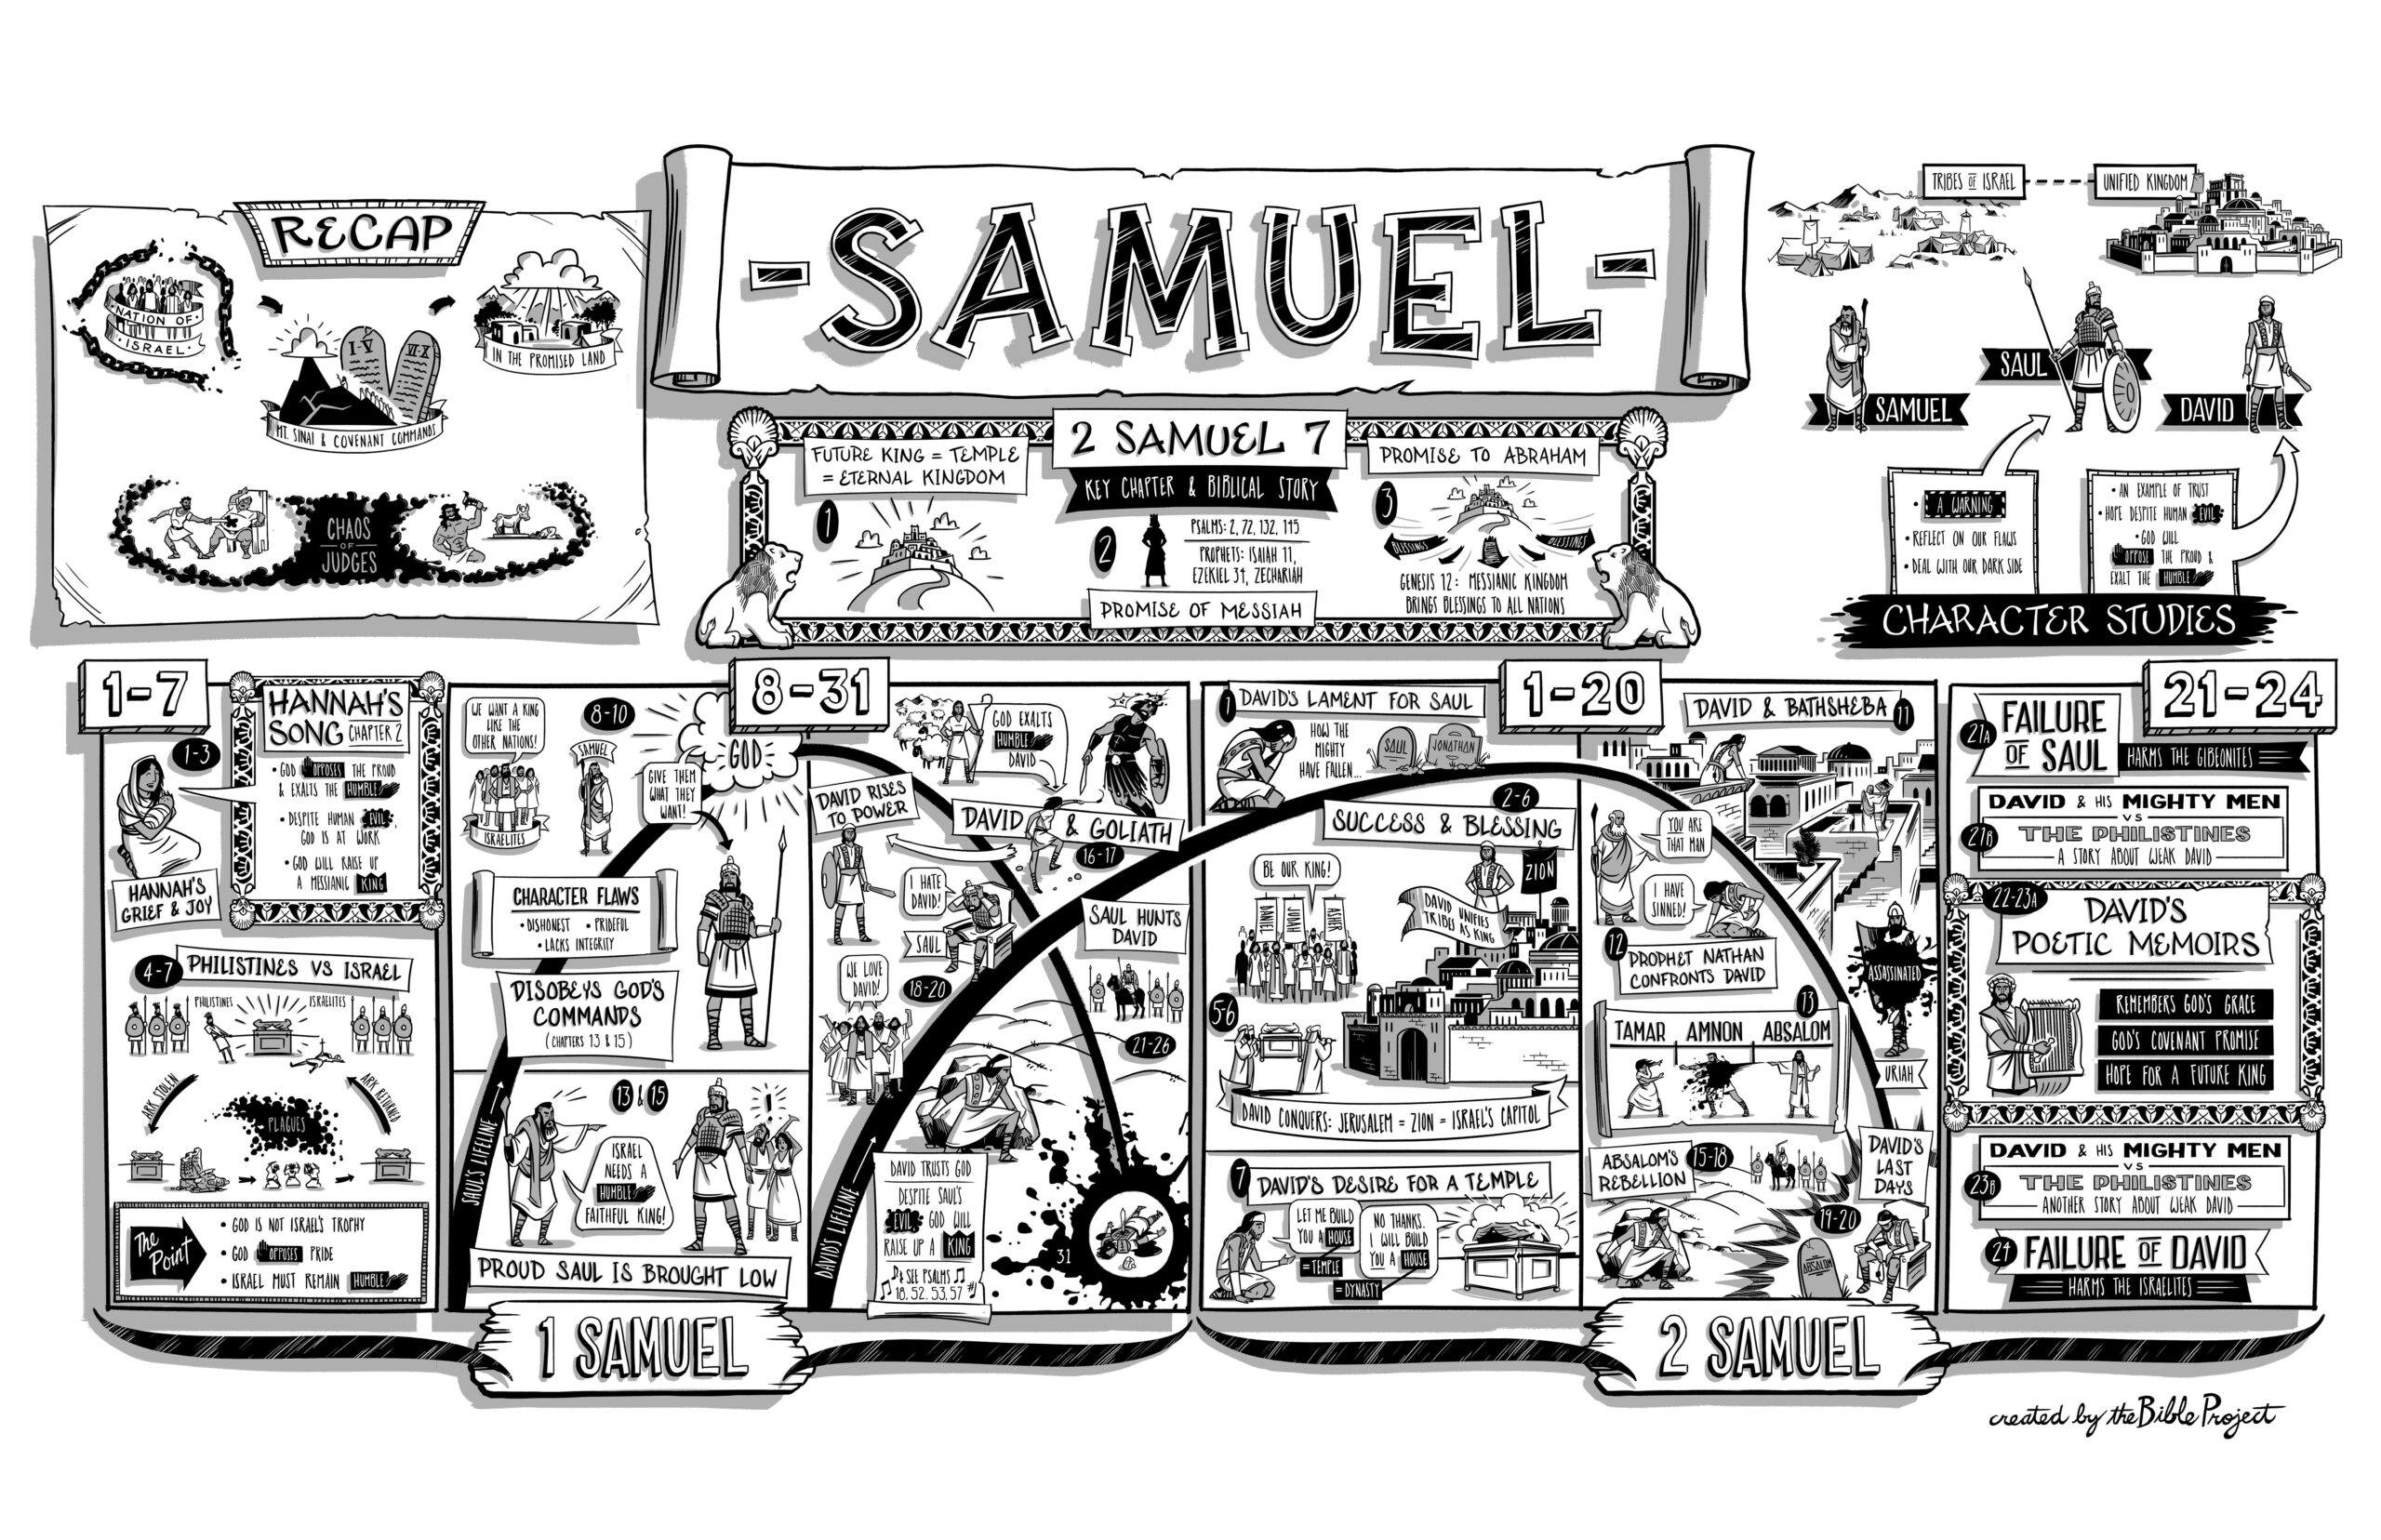
\includegraphics[scale=0.2, angle=90]{10OT-2Samuel/References/BibleProject-1-2Samuel.jpg}
\caption[1 and 2 Samuel from the Bible Project]{1 and 2 Samuel from the Bible Project}
\label{fig:1 and 2 Samuel from the Bible Project}
\end{center}
\end{figure}

\newpage
\begin{figure}
\begin{center}
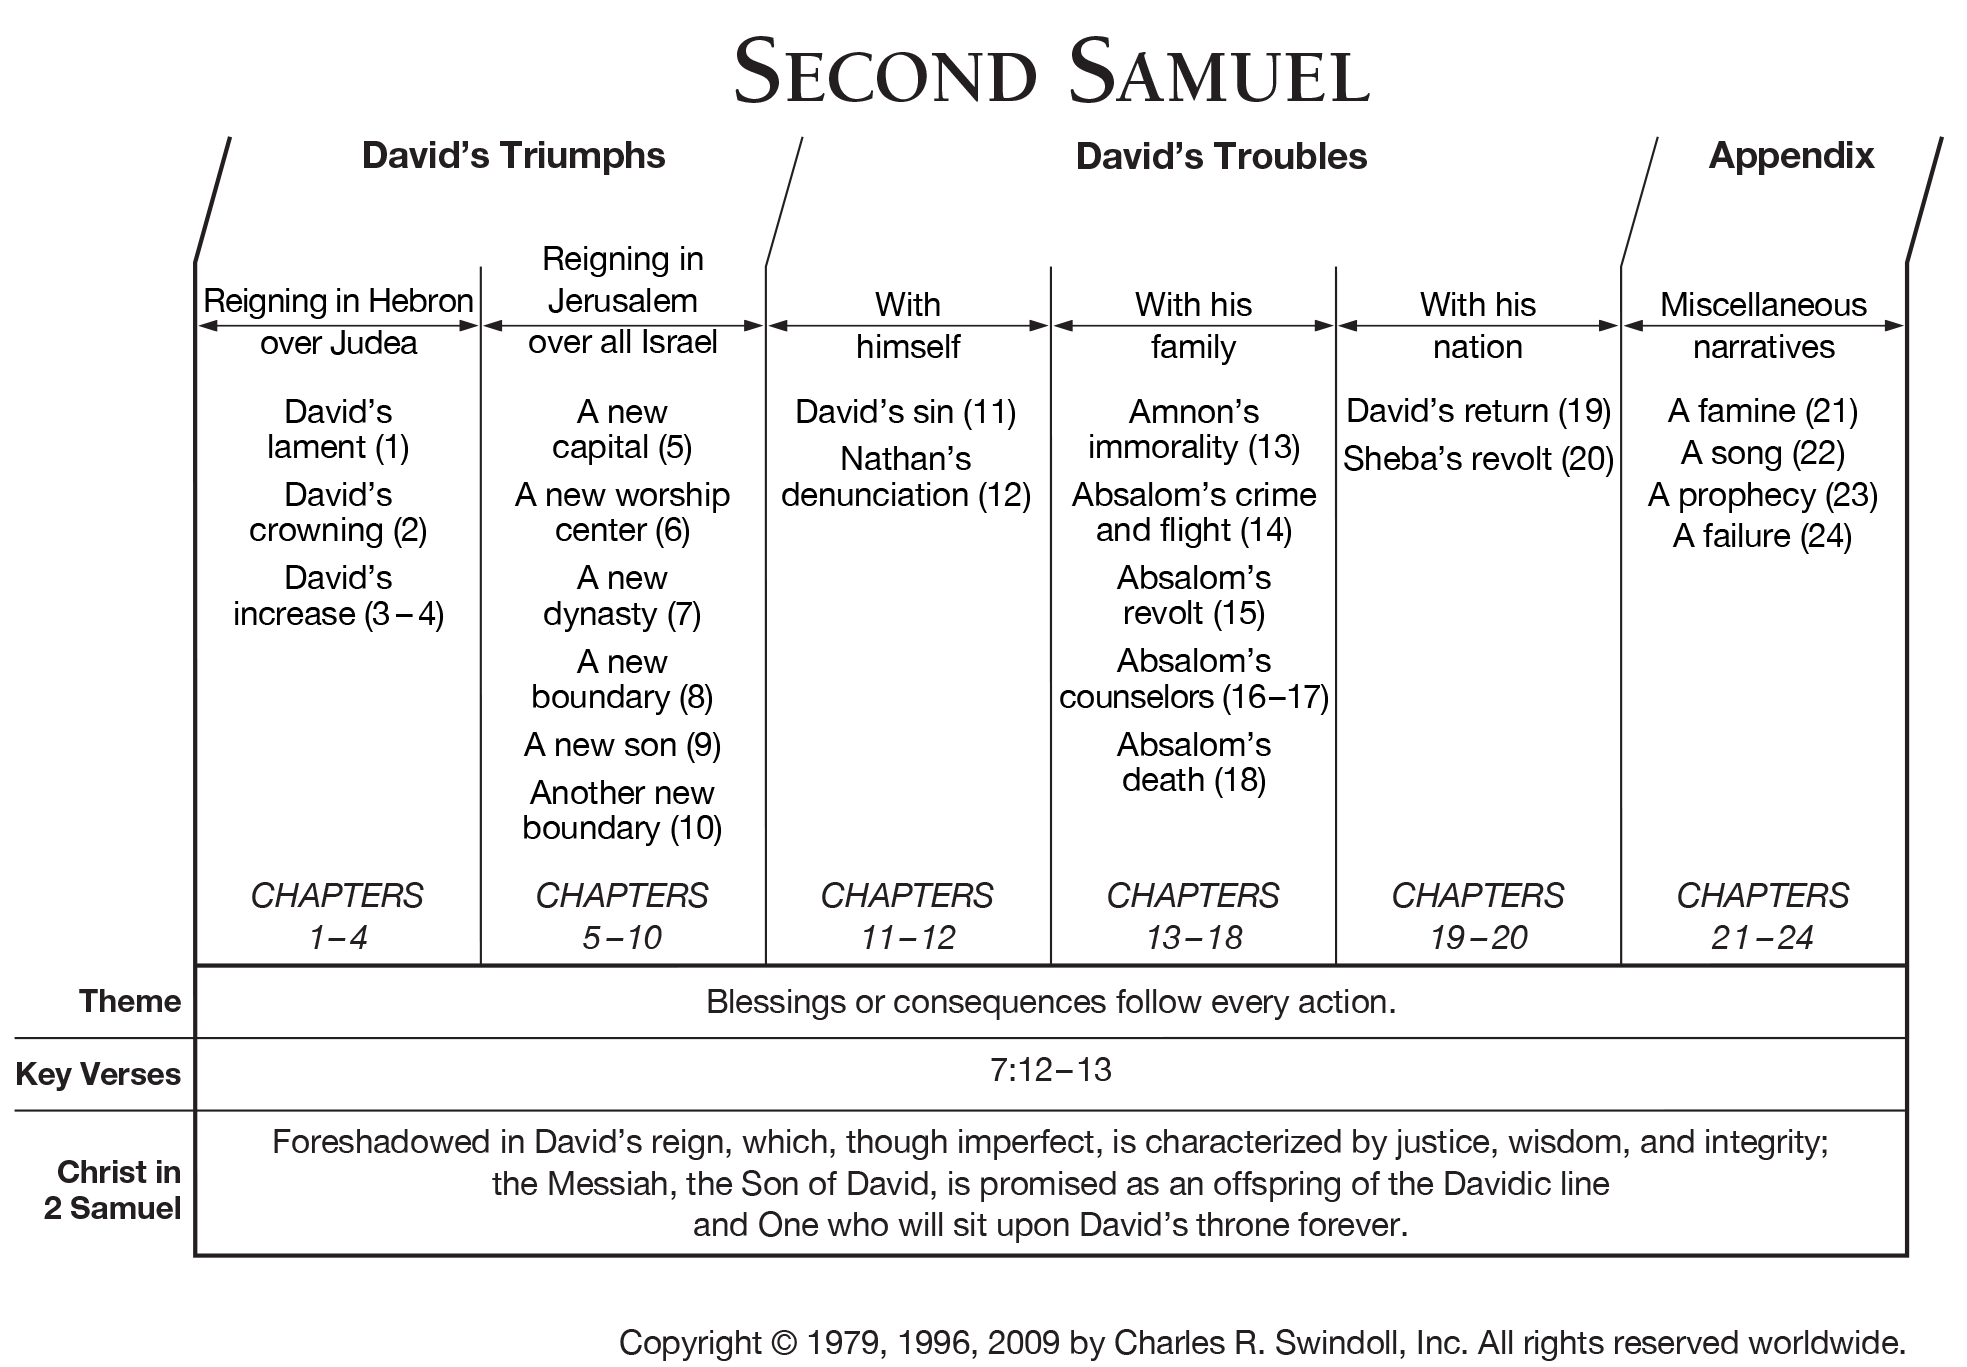
\includegraphics[scale=0.275, angle=90]{10OT-2Samuel/References/Swindoll-2Samuel.png}
\caption[2 Samuel by Swindoll]{2 Samuel by Swindoll}
\label{fig:2 Samuel by Swindoll}
\end{center}
\end{figure}

\newpage
\begin{figure}
\begin{center}
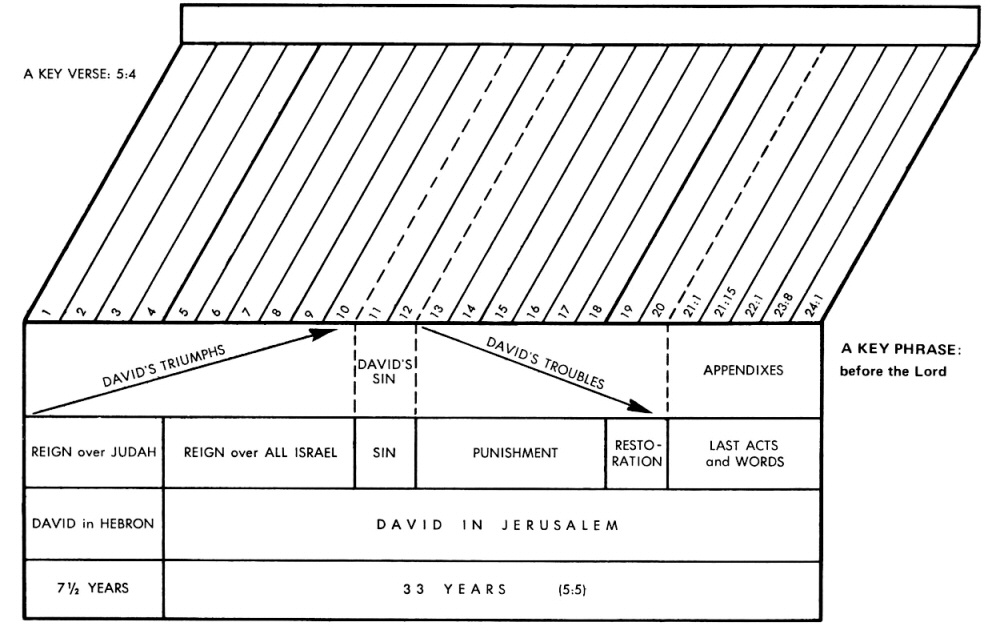
\includegraphics[scale=1.5, angle=90]{10OT-2Samuel/References/Jensen-2Samuel.png}
\caption[2 Samuel by Jensen]{2 Samuel by Jensen}
\label{fig:2 Samuel by Jensen}
\end{center}
\end{figure}


\newpage
\begin{figure}
\begin{center}
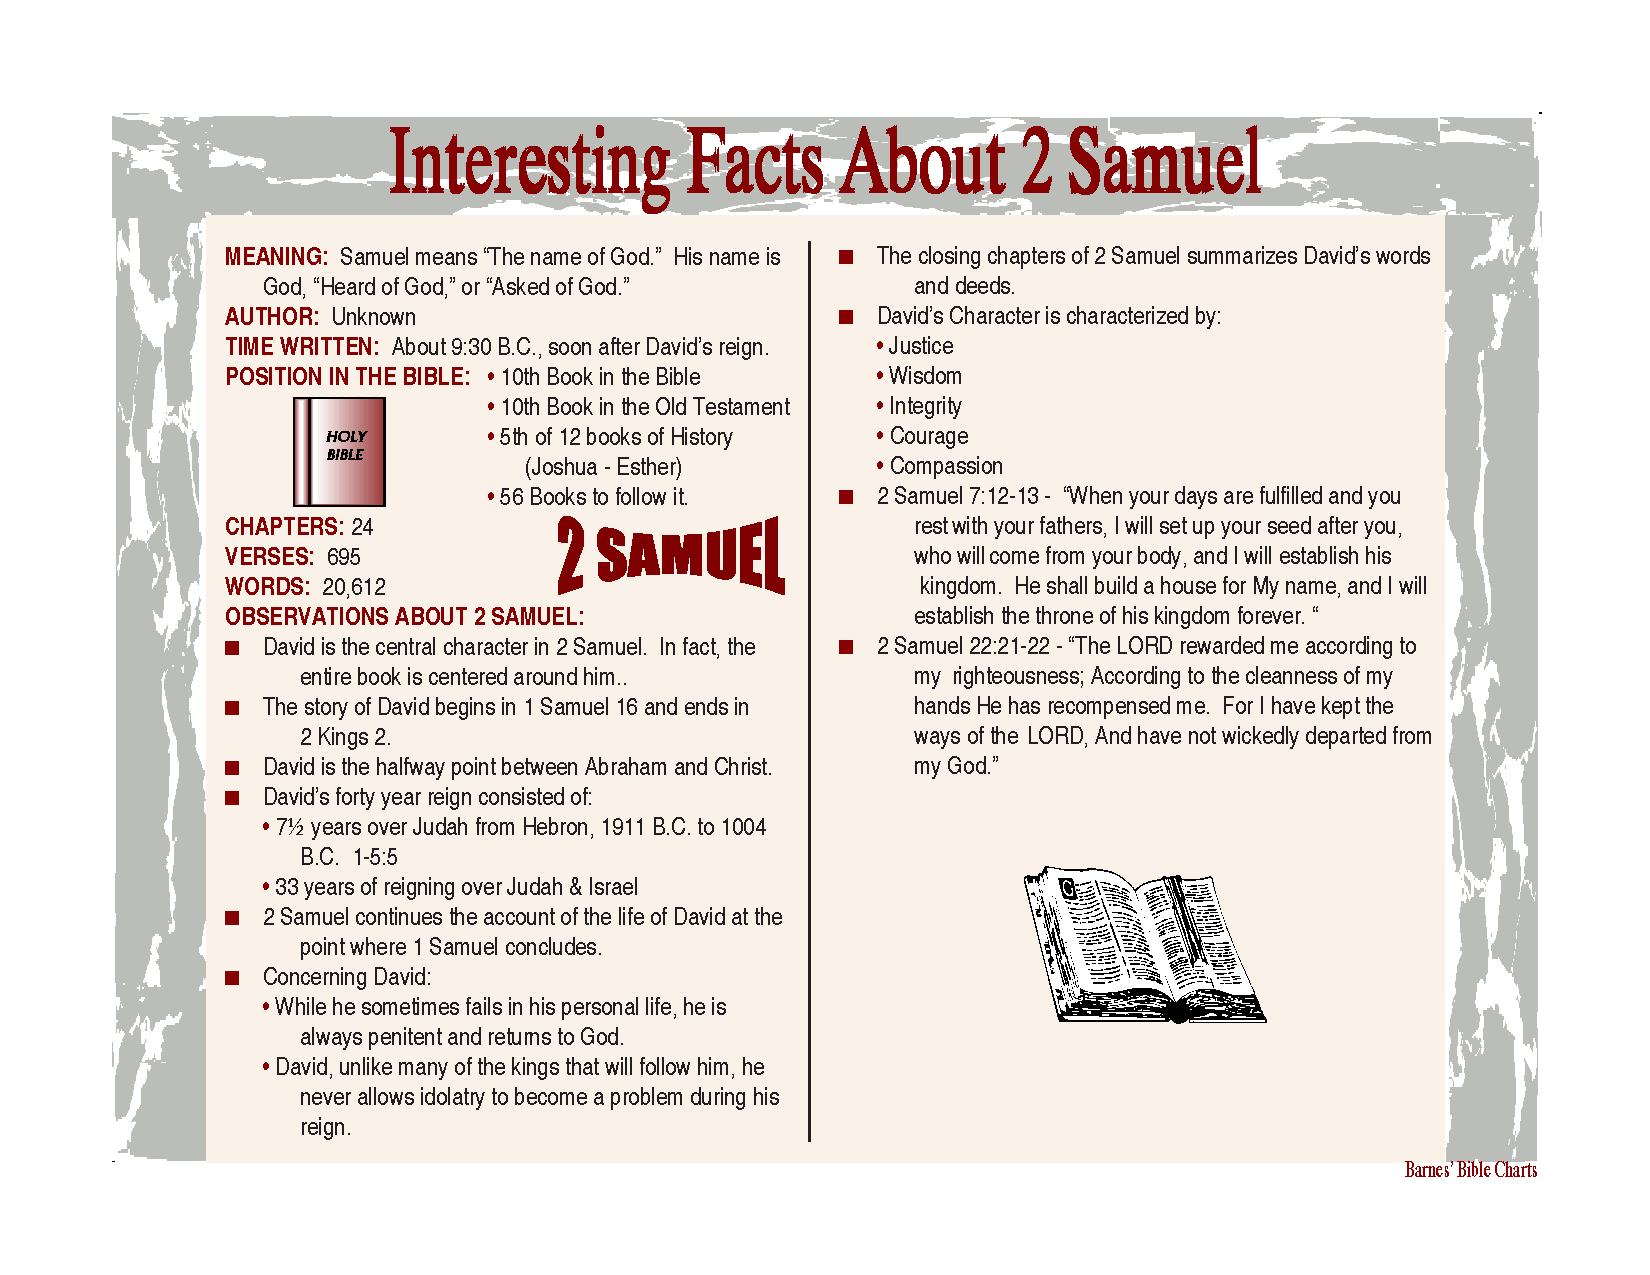
\includegraphics[scale=0.5, angle=0]{10OT-2Samuel/References/interestingfactsaboutsecondsamuel.pdf}
\caption[Interesting Facts about 2 Samuel]{Interesting Facts about 2 Samuel}
\label{fig:Interesting Facts about 1 Samuel}
\end{center}
\end{figure}



\chapter{2 Samuel 22}

\begin{figure}
  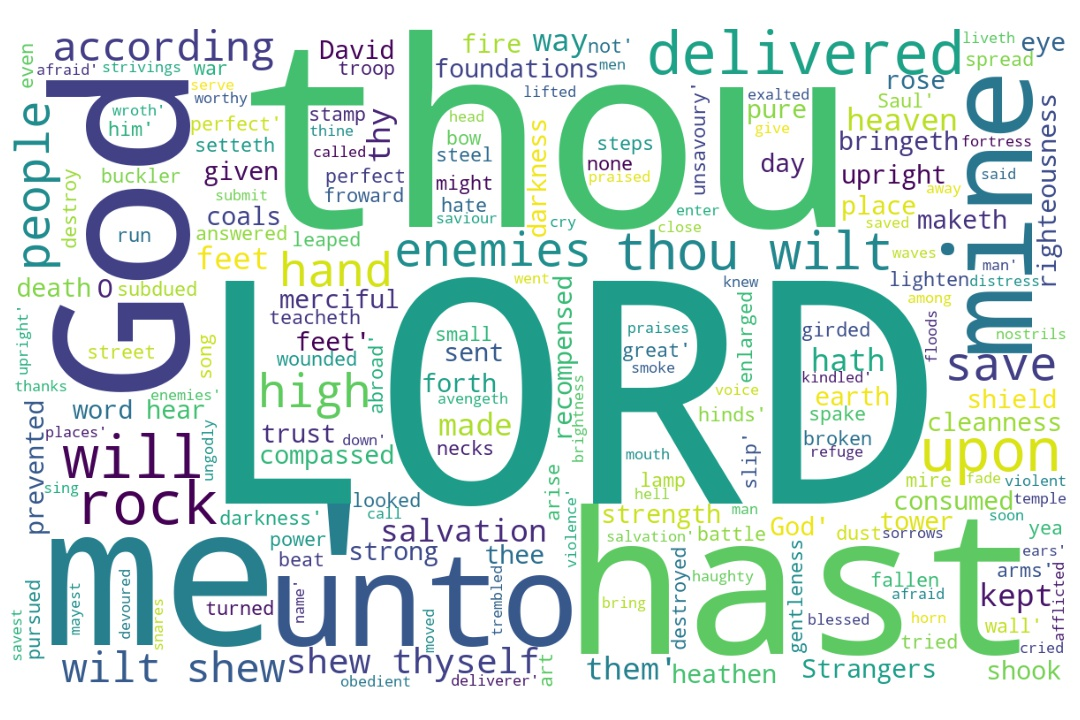
\includegraphics[width=\linewidth]{10OT-2Samuel/2Samuel22-WordCloud.jpg}
  \caption{1 Samuel 22 Word Cloud}
  \label{fig:1 Samuel 22 Word Cloud}
\end{figure}

%%%%%%%%%%%%%%%%%%%%%%%%%%%%%%%%%%%%%%%%%
%%%%%%%%%%%%%%%%%%%%%%%%%%%%%%%%%%%%%%%%%

\marginpar{\scriptsize \centering \fcolorbox{bone}{lime}{\textbf{DAVID"S REFLECTION}}\\ (2 Samuel 22:1--51) 
\begin{compactenum}[I.][8]
    \item David as a  \textbf{Vessel} %\index[scripture]{2Samuel!2Sa 22:01}(2Sa 22:1) 
    \item Two \textbf{Voices}  \index[scripture]{2Samuel!2Sa 22:07}  \index[scripture]{2Samuel!2Sa 22:14} (2Sa 22:7, 14) 
    \item The \textbf{Virtue} (or lack thereof, and the rewards thereof, but the repentance \index[scripture]{2Samuel!2Sa 22:22--26}(2Sa  22:22--26) 
    \item God's Care for \textbf{Victims}  \index[scripture]{2Samuel!2Sa 22:28}(2Sa 22:28) 
    \item The \textbf{Victories}  \index[scripture]{2Samuel!2Sa 22:40}(2Sa 22:40) 
    \item An \textbf{Avenging}  \index[scripture]{2Samuel!2Sa 22:48}(2Sa 22:48) 
    \item Deliverance from the  \textbf{Violent}  \index[scripture]{2Samuel!2Sa 22:49}(2Sa 22:49) 
\end{compactenum} }

\footnote{\textcolor[cmyk]{0.99998,1,0,0}{\hyperlink{TOC}{Return to end of Table of Contents.}}}\footnote{\href{https://audiobible.com/bible/2_samuel_22.html}{\textcolor[cmyk]{0.99998,1,0,0}{2 Samuel 22 Audio}}}\textcolor[cmyk]{0.99998,1,0,0}{And David spake unto the LORD the words of this song in the day \emph{that} the LORD had delivered him out of the hand of all his enemies, and out of the hand of Saul:}
[2] \textcolor[cmyk]{0.99998,1,0,0}{And he said, The LORD \emph{is} my rock, and my fortress, and my deliverer;}
[3] \textcolor[cmyk]{0.99998,1,0,0}{The God of my rock; in him will I trust: \emph{he} \emph{is} my shield, and the horn of my salvation, my high tower, and my refuge, my saviour; \fcolorbox{bone}{bone}{thou}  savest me from violence.}
[4] \textcolor[cmyk]{0.99998,1,0,0}{I will call on the LORD, \emph{who} \emph{is} worthy to be praised: so shall I be saved from mine enemies.}
[5] \textcolor[cmyk]{0.99998,1,0,0}{When the waves of death compassed me, the floods of ungodly men made me afraid;}
[6] \textcolor[cmyk]{0.99998,1,0,0}{The sorrows of hell compassed me about; the snares of death prevented me;}
[7] \textcolor[cmyk]{0.99998,1,0,0}{In my distress I called upon the LORD, and cried to my God: and he did hear \fcolorbox{bone}{lime}{my voice} out of his temple, and my cry \emph{did} \emph{enter} into his ears.}
[8] \textcolor[cmyk]{0.99998,1,0,0}{Then the earth shook and trembled; the foundations of heaven moved and shook, because he was wroth.}
[9] \textcolor[cmyk]{0.99998,1,0,0}{There went up a smoke out of his nostrils, and fire out of his mouth devoured: coals were kindled by it.}
[10] \textcolor[cmyk]{0.99998,1,0,0}{He bowed the heavens also, and came down; and darkness \emph{was} under his feet.}
[11] \textcolor[cmyk]{0.99998,1,0,0}{And he rode upon a cherub, and did fly: and he was seen upon the wings of the wind.}
[12] \textcolor[cmyk]{0.99998,1,0,0}{And he made darkness pavilions round about him, dark waters, \emph{and} thick clouds of the skies.}
[13] \textcolor[cmyk]{0.99998,1,0,0}{Through the brightness before him were coals of fire kindled.}
[14] \textcolor[cmyk]{0.99998,1,0,0}{The LORD thundered from heaven, and the most High uttered \fcolorbox{bone}{lime}{his voice}.}
[15] \textcolor[cmyk]{0.99998,1,0,0}{And he sent out arrows, and scattered them; lightning, and discomfited them.}
[16] \textcolor[cmyk]{0.99998,1,0,0}{And the channels of the sea appeared, the foundations of the world were discovered, at the rebuking of the LORD, at the blast of the breath of his nostrils.}
[17] \textcolor[cmyk]{0.99998,1,0,0}{He sent from above, he took me; he drew me out of many waters;}
[18] \textcolor[cmyk]{0.99998,1,0,0}{He delivered me from my strong enemy, \emph{and} from them that hated me: for they were too strong for me.}
[19] \textcolor[cmyk]{0.99998,1,0,0}{They prevented me in the day of my calamity: but the LORD was my stay.}
[20] \textcolor[cmyk]{0.99998,1,0,0}{He brought me forth also into a large place: he delivered me, because he delighted in me.}
[21] \textcolor[cmyk]{0.99998,1,0,0}{The LORD rewarded me according to my righteousness: according to the cleanness of my hands hath he recompensed me.}
[22] \textcolor[cmyk]{0.99998,1,0,0}{For I have kept the ways of the LORD, and have \fcolorbox{bone}{lime}{not wickedly departed} from my God.}
[23] \textcolor[cmyk]{0.99998,1,0,0}{For all his judgments \emph{were} before me: and \emph{as} \emph{for} his statutes, I did not depart from them.}
[24] \textcolor[cmyk]{0.99998,1,0,0}{I was also upright before him, and have kept myself from mine iniquity.}
[25] \textcolor[cmyk]{0.99998,1,0,0}{Therefore the LORD hath recompensed me according to my righteousness; according to my cleanness in his eye sight.}
[26] \textcolor[cmyk]{0.99998,1,0,0}{With the merciful \fcolorbox{bone}{bone}{thou}  wilt shew thyself merciful, \emph{and} with the upright man \fcolorbox{bone}{bone}{thou}  wilt shew thyself upright.}
[27] \textcolor[cmyk]{0.99998,1,0,0}{With the pure \fcolorbox{bone}{bone}{thou}  wilt shew thyself pure; and with the froward \fcolorbox{bone}{bone}{thou}  wilt shew thyself unsavoury.}
[28] \textcolor[cmyk]{0.99998,1,0,0}{And \fcolorbox{bone}{lime}{the afflicted people} \fcolorbox{bone}{bone}{thou}  wilt save: but thine eyes \emph{are} upon the haughty, \emph{that} \fcolorbox{bone}{bone}{thou}  mayest bring \emph{them} down.}
[29] \textcolor[cmyk]{0.99998,1,0,0}{For \fcolorbox{bone}{bone}{thou}  \emph{art} my lamp, O LORD: and the LORD will lighten my darkness.}
[30] \textcolor[cmyk]{0.99998,1,0,0}{For by thee I have run through a troop: by my God have I leaped over a wall.}
[31] \textcolor[cmyk]{0.99998,1,0,0}{\emph{As} \emph{for} God, his way \emph{is} perfect; the word of the LORD \emph{is} tried: he \emph{is} a buckler to all them that trust in him.}
[32] \textcolor[cmyk]{0.99998,1,0,0}{For who \emph{is} God, save the LORD? and who \emph{is} a rock, save our God?}
[33] \textcolor[cmyk]{0.99998,1,0,0}{God \emph{is} my strength \emph{and} power: and he maketh my way perfect.}
[34] \textcolor[cmyk]{0.99998,1,0,0}{He maketh my feet like hinds' \emph{feet}: and setteth me upon my high places.}
[35] \textcolor[cmyk]{0.99998,1,0,0}{He teacheth my hands to war; so that a bow of steel is broken by mine arms.}
[36] \textcolor[cmyk]{0.99998,1,0,0}{Thou hast also given me the shield of thy salvation: and thy gentleness hath made me great.}
[37] \textcolor[cmyk]{0.99998,1,0,0}{Thou hast enlarged my steps under me; so that my feet did not slip.}
[38] \textcolor[cmyk]{0.99998,1,0,0}{I have pursued mine enemies, and destroyed them; and turned not again until I had consumed them.}
[39] \textcolor[cmyk]{0.99998,1,0,0}{And I have consumed them, and wounded them, that they could not arise: yea, they are fallen under my feet.}
[40] \textcolor[cmyk]{0.99998,1,0,0}{For \fcolorbox{bone}{bone}{thou}  hast girded me with strength to battle: them that rose up against me \fcolorbox{bone}{lime}{hast \fcolorbox{bone}{bone}{thou}  subdued} under me.}
[41] \textcolor[cmyk]{0.99998,1,0,0}{Thou hast also given me the necks of mine enemies, that I might destroy them that hate me.}
[42] \textcolor[cmyk]{0.99998,1,0,0}{They looked, but \emph{there} \emph{was} none to save; \emph{even} unto the LORD, but he answered them not.}
[43] \textcolor[cmyk]{0.99998,1,0,0}{Then did I beat them as small as the dust of the earth, I did stamp them as the mire of the street, \emph{and} did spread them abroad.}
[44] \textcolor[cmyk]{0.99998,1,0,0}{Thou also hast delivered me from the strivings of my people, \fcolorbox{bone}{bone}{thou}  hast kept me \emph{to} \emph{be} head of the heathen: a people \emph{which} I knew not shall serve me.}
[45] \textcolor[cmyk]{0.99998,1,0,0}{Strangers shall submit themselves unto me: as soon as they hear, they shall be obedient unto me.}
[46] \textcolor[cmyk]{0.99998,1,0,0}{Strangers shall fade away, and they shall be afraid out of their close places.}
[47] \textcolor[cmyk]{0.99998,1,0,0}{The LORD liveth; and blessed \emph{be} my rock; and exalted be the God of the rock of my salvation.}
[48] \textcolor[cmyk]{0.99998,1,0,0}{It \emph{is} God that \fcolorbox{bone}{lime}{avengeth} me, and that bringeth down the people under me,}
[49] \textcolor[cmyk]{0.99998,1,0,0}{And that bringeth me forth \fcolorbox{bone}{lime}{from mine enemies}: \fcolorbox{bone}{bone}{thou}  also hast lifted me up on high above them that rose up against me: \fcolorbox{bone}{bone}{thou}  hast delivered me from the violent man.}
[50] \textcolor[cmyk]{0.99998,1,0,0}{Therefore I will give thanks unto thee, O LORD, among the heathen, and I will sing praises unto thy name.}
[51] \textcolor[cmyk]{0.99998,1,0,0}{\emph{He} \emph{is} the tower of salvation for his king: and sheweth mercy to his anointed, unto David, and to his seed for evermore.}
\index[NWIV]{35!2Samuel!2Sa 22:1}\index[AWIP]{And!2Samuel!2Sa 22:1}\index[AWIP]{David!2Samuel!2Sa 22:1}\index[AWIP]{spake!2Samuel!2Sa 22:1}\index[AWIP]{unto!2Samuel!2Sa 22:1}\index[AWIP]{the!2Samuel!2Sa 22:1}\index[AWIP]{the!2Samuel!2Sa 22:1 (2)}\index[AWIP]{the!2Samuel!2Sa 22:1 (3)}\index[AWIP]{the!2Samuel!2Sa 22:1 (4)}\index[AWIP]{the!2Samuel!2Sa 22:1 (5)}\index[AWIP]{the!2Samuel!2Sa 22:1 (6)}\index[AWIP]{LORD!2Samuel!2Sa 22:1}\index[AWIP]{LORD!2Samuel!2Sa 22:1 (2)}\index[AWIP]{words!2Samuel!2Sa 22:1}\index[AWIP]{of!2Samuel!2Sa 22:1}\index[AWIP]{of!2Samuel!2Sa 22:1 (2)}\index[AWIP]{of!2Samuel!2Sa 22:1 (3)}\index[AWIP]{of!2Samuel!2Sa 22:1 (4)}\index[AWIP]{of!2Samuel!2Sa 22:1 (5)}\index[AWIP]{this!2Samuel!2Sa 22:1}\index[AWIP]{song!2Samuel!2Sa 22:1}\index[AWIP]{in!2Samuel!2Sa 22:1}\index[AWIP]{day!2Samuel!2Sa 22:1}\index[AWIP]{\emph{that}!2Samuel!2Sa 22:1}\index[AWIP]{had!2Samuel!2Sa 22:1}\index[AWIP]{delivered!2Samuel!2Sa 22:1}\index[AWIP]{him!2Samuel!2Sa 22:1}\index[AWIP]{out!2Samuel!2Sa 22:1}\index[AWIP]{out!2Samuel!2Sa 22:1 (2)}\index[AWIP]{hand!2Samuel!2Sa 22:1}\index[AWIP]{hand!2Samuel!2Sa 22:1 (2)}\index[AWIP]{all!2Samuel!2Sa 22:1}\index[AWIP]{his!2Samuel!2Sa 22:1}\index[AWIP]{enemies!2Samuel!2Sa 22:1}\index[AWIP]{and!2Samuel!2Sa 22:1}\index[AWIP]{Saul!2Samuel!2Sa 22:1}\index[AWIP]{\emph{that}!2Samuel!2Sa 22:1}

\index[NWIV]{14!2Samuel!2Sa 22:2}\index[AWIP]{And!2Samuel!2Sa 22:2}\index[AWIP]{he!2Samuel!2Sa 22:2}\index[AWIP]{said!2Samuel!2Sa 22:2}\index[AWIP]{The!2Samuel!2Sa 22:2}\index[AWIP]{LORD!2Samuel!2Sa 22:2}\index[AWIP]{\emph{is}!2Samuel!2Sa 22:2}\index[AWIP]{my!2Samuel!2Sa 22:2}\index[AWIP]{my!2Samuel!2Sa 22:2 (2)}\index[AWIP]{my!2Samuel!2Sa 22:2 (3)}\index[AWIP]{rock!2Samuel!2Sa 22:2}\index[AWIP]{and!2Samuel!2Sa 22:2}\index[AWIP]{and!2Samuel!2Sa 22:2 (2)}\index[AWIP]{fortress!2Samuel!2Sa 22:2}\index[AWIP]{deliverer!2Samuel!2Sa 22:2}\index[AWIP]{\emph{is}!2Samuel!2Sa 22:2}

\index[NWIV]{33!2Samuel!2Sa 22:3}\index[AWIP]{The!2Samuel!2Sa 22:3}\index[AWIP]{God!2Samuel!2Sa 22:3}\index[AWIP]{of!2Samuel!2Sa 22:3}\index[AWIP]{of!2Samuel!2Sa 22:3 (2)}\index[AWIP]{my!2Samuel!2Sa 22:3}\index[AWIP]{my!2Samuel!2Sa 22:3 (2)}\index[AWIP]{my!2Samuel!2Sa 22:3 (3)}\index[AWIP]{my!2Samuel!2Sa 22:3 (4)}\index[AWIP]{my!2Samuel!2Sa 22:3 (5)}\index[AWIP]{my!2Samuel!2Sa 22:3 (6)}\index[AWIP]{rock!2Samuel!2Sa 22:3}\index[AWIP]{in!2Samuel!2Sa 22:3}\index[AWIP]{him!2Samuel!2Sa 22:3}\index[AWIP]{will!2Samuel!2Sa 22:3}\index[AWIP]{I!2Samuel!2Sa 22:3}\index[AWIP]{trust!2Samuel!2Sa 22:3}\index[AWIP]{\emph{he}!2Samuel!2Sa 22:3}\index[AWIP]{\emph{is}!2Samuel!2Sa 22:3}\index[AWIP]{shield!2Samuel!2Sa 22:3}\index[AWIP]{and!2Samuel!2Sa 22:3}\index[AWIP]{and!2Samuel!2Sa 22:3 (2)}\index[AWIP]{the!2Samuel!2Sa 22:3}\index[AWIP]{horn!2Samuel!2Sa 22:3}\index[AWIP]{salvation!2Samuel!2Sa 22:3}\index[AWIP]{high!2Samuel!2Sa 22:3}\index[AWIP]{tower!2Samuel!2Sa 22:3}\index[AWIP]{refuge!2Samuel!2Sa 22:3}\index[AWIP]{saviour!2Samuel!2Sa 22:3}\index[AWIP]{thou!2Samuel!2Sa 22:3}\index[AWIP]{savest!2Samuel!2Sa 22:3}\index[AWIP]{me!2Samuel!2Sa 22:3}\index[AWIP]{from!2Samuel!2Sa 22:3}\index[AWIP]{violence!2Samuel!2Sa 22:3}\index[AWIP]{\emph{he}!2Samuel!2Sa 22:3}\index[AWIP]{\emph{is}!2Samuel!2Sa 22:3}

\index[NWIV]{20!2Samuel!2Sa 22:4}\index[AWIP]{I!2Samuel!2Sa 22:4}\index[AWIP]{I!2Samuel!2Sa 22:4 (2)}\index[AWIP]{will!2Samuel!2Sa 22:4}\index[AWIP]{call!2Samuel!2Sa 22:4}\index[AWIP]{on!2Samuel!2Sa 22:4}\index[AWIP]{the!2Samuel!2Sa 22:4}\index[AWIP]{LORD!2Samuel!2Sa 22:4}\index[AWIP]{\emph{who}!2Samuel!2Sa 22:4}\index[AWIP]{\emph{is}!2Samuel!2Sa 22:4}\index[AWIP]{worthy!2Samuel!2Sa 22:4}\index[AWIP]{to!2Samuel!2Sa 22:4}\index[AWIP]{be!2Samuel!2Sa 22:4}\index[AWIP]{be!2Samuel!2Sa 22:4 (2)}\index[AWIP]{praised!2Samuel!2Sa 22:4}\index[AWIP]{so!2Samuel!2Sa 22:4}\index[AWIP]{shall!2Samuel!2Sa 22:4}\index[AWIP]{saved!2Samuel!2Sa 22:4}\index[AWIP]{from!2Samuel!2Sa 22:4}\index[AWIP]{mine!2Samuel!2Sa 22:4}\index[AWIP]{enemies!2Samuel!2Sa 22:4}\index[AWIP]{\emph{who}!2Samuel!2Sa 22:4}\index[AWIP]{\emph{is}!2Samuel!2Sa 22:4}

\index[NWIV]{15!2Samuel!2Sa 22:5}\index[AWIP]{When!2Samuel!2Sa 22:5}\index[AWIP]{the!2Samuel!2Sa 22:5}\index[AWIP]{the!2Samuel!2Sa 22:5 (2)}\index[AWIP]{waves!2Samuel!2Sa 22:5}\index[AWIP]{of!2Samuel!2Sa 22:5}\index[AWIP]{of!2Samuel!2Sa 22:5 (2)}\index[AWIP]{death!2Samuel!2Sa 22:5}\index[AWIP]{compassed!2Samuel!2Sa 22:5}\index[AWIP]{me!2Samuel!2Sa 22:5}\index[AWIP]{me!2Samuel!2Sa 22:5 (2)}\index[AWIP]{floods!2Samuel!2Sa 22:5}\index[AWIP]{ungodly!2Samuel!2Sa 22:5}\index[AWIP]{men!2Samuel!2Sa 22:5}\index[AWIP]{made!2Samuel!2Sa 22:5}\index[AWIP]{afraid!2Samuel!2Sa 22:5}

\index[NWIV]{13!2Samuel!2Sa 22:6}\index[AWIP]{The!2Samuel!2Sa 22:6}\index[AWIP]{sorrows!2Samuel!2Sa 22:6}\index[AWIP]{of!2Samuel!2Sa 22:6}\index[AWIP]{of!2Samuel!2Sa 22:6 (2)}\index[AWIP]{hell!2Samuel!2Sa 22:6}\index[AWIP]{compassed!2Samuel!2Sa 22:6}\index[AWIP]{me!2Samuel!2Sa 22:6}\index[AWIP]{me!2Samuel!2Sa 22:6 (2)}\index[AWIP]{about!2Samuel!2Sa 22:6}\index[AWIP]{the!2Samuel!2Sa 22:6}\index[AWIP]{snares!2Samuel!2Sa 22:6}\index[AWIP]{death!2Samuel!2Sa 22:6}\index[AWIP]{prevented!2Samuel!2Sa 22:6}

\index[NWIV]{31!2Samuel!2Sa 22:7}\index[AWIP]{In!2Samuel!2Sa 22:7}\index[AWIP]{my!2Samuel!2Sa 22:7}\index[AWIP]{my!2Samuel!2Sa 22:7 (2)}\index[AWIP]{my!2Samuel!2Sa 22:7 (3)}\index[AWIP]{my!2Samuel!2Sa 22:7 (4)}\index[AWIP]{distress!2Samuel!2Sa 22:7}\index[AWIP]{I!2Samuel!2Sa 22:7}\index[AWIP]{called!2Samuel!2Sa 22:7}\index[AWIP]{upon!2Samuel!2Sa 22:7}\index[AWIP]{the!2Samuel!2Sa 22:7}\index[AWIP]{LORD!2Samuel!2Sa 22:7}\index[AWIP]{and!2Samuel!2Sa 22:7}\index[AWIP]{and!2Samuel!2Sa 22:7 (2)}\index[AWIP]{and!2Samuel!2Sa 22:7 (3)}\index[AWIP]{cried!2Samuel!2Sa 22:7}\index[AWIP]{to!2Samuel!2Sa 22:7}\index[AWIP]{God!2Samuel!2Sa 22:7}\index[AWIP]{he!2Samuel!2Sa 22:7}\index[AWIP]{did!2Samuel!2Sa 22:7}\index[AWIP]{hear!2Samuel!2Sa 22:7}\index[AWIP]{voice!2Samuel!2Sa 22:7}\index[AWIP]{out!2Samuel!2Sa 22:7}\index[AWIP]{of!2Samuel!2Sa 22:7}\index[AWIP]{his!2Samuel!2Sa 22:7}\index[AWIP]{his!2Samuel!2Sa 22:7 (2)}\index[AWIP]{temple!2Samuel!2Sa 22:7}\index[AWIP]{cry!2Samuel!2Sa 22:7}\index[AWIP]{\emph{did}!2Samuel!2Sa 22:7}\index[AWIP]{\emph{enter}!2Samuel!2Sa 22:7}\index[AWIP]{into!2Samuel!2Sa 22:7}\index[AWIP]{ears!2Samuel!2Sa 22:7}\index[AWIP]{\emph{did}!2Samuel!2Sa 22:7}\index[AWIP]{\emph{enter}!2Samuel!2Sa 22:7}

\index[NWIV]{17!2Samuel!2Sa 22:8}\index[AWIP]{Then!2Samuel!2Sa 22:8}\index[AWIP]{the!2Samuel!2Sa 22:8}\index[AWIP]{the!2Samuel!2Sa 22:8 (2)}\index[AWIP]{earth!2Samuel!2Sa 22:8}\index[AWIP]{shook!2Samuel!2Sa 22:8}\index[AWIP]{shook!2Samuel!2Sa 22:8 (2)}\index[AWIP]{and!2Samuel!2Sa 22:8}\index[AWIP]{and!2Samuel!2Sa 22:8 (2)}\index[AWIP]{trembled!2Samuel!2Sa 22:8}\index[AWIP]{foundations!2Samuel!2Sa 22:8}\index[AWIP]{of!2Samuel!2Sa 22:8}\index[AWIP]{heaven!2Samuel!2Sa 22:8}\index[AWIP]{moved!2Samuel!2Sa 22:8}\index[AWIP]{because!2Samuel!2Sa 22:8}\index[AWIP]{he!2Samuel!2Sa 22:8}\index[AWIP]{was!2Samuel!2Sa 22:8}\index[AWIP]{wroth!2Samuel!2Sa 22:8}

\index[NWIV]{21!2Samuel!2Sa 22:9}\index[AWIP]{There!2Samuel!2Sa 22:9}\index[AWIP]{went!2Samuel!2Sa 22:9}\index[AWIP]{up!2Samuel!2Sa 22:9}\index[AWIP]{a!2Samuel!2Sa 22:9}\index[AWIP]{smoke!2Samuel!2Sa 22:9}\index[AWIP]{out!2Samuel!2Sa 22:9}\index[AWIP]{out!2Samuel!2Sa 22:9 (2)}\index[AWIP]{of!2Samuel!2Sa 22:9}\index[AWIP]{of!2Samuel!2Sa 22:9 (2)}\index[AWIP]{his!2Samuel!2Sa 22:9}\index[AWIP]{his!2Samuel!2Sa 22:9 (2)}\index[AWIP]{nostrils!2Samuel!2Sa 22:9}\index[AWIP]{and!2Samuel!2Sa 22:9}\index[AWIP]{fire!2Samuel!2Sa 22:9}\index[AWIP]{mouth!2Samuel!2Sa 22:9}\index[AWIP]{devoured!2Samuel!2Sa 22:9}\index[AWIP]{coals!2Samuel!2Sa 22:9}\index[AWIP]{were!2Samuel!2Sa 22:9}\index[AWIP]{kindled!2Samuel!2Sa 22:9}\index[AWIP]{by!2Samuel!2Sa 22:9}\index[AWIP]{it!2Samuel!2Sa 22:9}

\index[NWIV]{14!2Samuel!2Sa 22:10}\index[AWIP]{He!2Samuel!2Sa 22:10}\index[AWIP]{bowed!2Samuel!2Sa 22:10}\index[AWIP]{the!2Samuel!2Sa 22:10}\index[AWIP]{heavens!2Samuel!2Sa 22:10}\index[AWIP]{also!2Samuel!2Sa 22:10}\index[AWIP]{and!2Samuel!2Sa 22:10}\index[AWIP]{and!2Samuel!2Sa 22:10 (2)}\index[AWIP]{came!2Samuel!2Sa 22:10}\index[AWIP]{down!2Samuel!2Sa 22:10}\index[AWIP]{darkness!2Samuel!2Sa 22:10}\index[AWIP]{\emph{was}!2Samuel!2Sa 22:10}\index[AWIP]{under!2Samuel!2Sa 22:10}\index[AWIP]{his!2Samuel!2Sa 22:10}\index[AWIP]{feet!2Samuel!2Sa 22:10}\index[AWIP]{\emph{was}!2Samuel!2Sa 22:10}

\index[NWIV]{19!2Samuel!2Sa 22:11}\index[AWIP]{And!2Samuel!2Sa 22:11}\index[AWIP]{he!2Samuel!2Sa 22:11}\index[AWIP]{he!2Samuel!2Sa 22:11 (2)}\index[AWIP]{rode!2Samuel!2Sa 22:11}\index[AWIP]{upon!2Samuel!2Sa 22:11}\index[AWIP]{upon!2Samuel!2Sa 22:11 (2)}\index[AWIP]{a!2Samuel!2Sa 22:11}\index[AWIP]{cherub!2Samuel!2Sa 22:11}\index[AWIP]{and!2Samuel!2Sa 22:11}\index[AWIP]{and!2Samuel!2Sa 22:11 (2)}\index[AWIP]{did!2Samuel!2Sa 22:11}\index[AWIP]{fly!2Samuel!2Sa 22:11}\index[AWIP]{was!2Samuel!2Sa 22:11}\index[AWIP]{seen!2Samuel!2Sa 22:11}\index[AWIP]{the!2Samuel!2Sa 22:11}\index[AWIP]{the!2Samuel!2Sa 22:11 (2)}\index[AWIP]{wings!2Samuel!2Sa 22:11}\index[AWIP]{of!2Samuel!2Sa 22:11}\index[AWIP]{wind!2Samuel!2Sa 22:11}

\index[NWIV]{16!2Samuel!2Sa 22:12}\index[AWIP]{And!2Samuel!2Sa 22:12}\index[AWIP]{he!2Samuel!2Sa 22:12}\index[AWIP]{made!2Samuel!2Sa 22:12}\index[AWIP]{darkness!2Samuel!2Sa 22:12}\index[AWIP]{pavilions!2Samuel!2Sa 22:12}\index[AWIP]{round!2Samuel!2Sa 22:12}\index[AWIP]{about!2Samuel!2Sa 22:12}\index[AWIP]{him!2Samuel!2Sa 22:12}\index[AWIP]{dark!2Samuel!2Sa 22:12}\index[AWIP]{waters!2Samuel!2Sa 22:12}\index[AWIP]{\emph{and}!2Samuel!2Sa 22:12}\index[AWIP]{thick!2Samuel!2Sa 22:12}\index[AWIP]{clouds!2Samuel!2Sa 22:12}\index[AWIP]{of!2Samuel!2Sa 22:12}\index[AWIP]{the!2Samuel!2Sa 22:12}\index[AWIP]{skies!2Samuel!2Sa 22:12}\index[AWIP]{\emph{and}!2Samuel!2Sa 22:12}

\index[NWIV]{10!2Samuel!2Sa 22:13}\index[AWIP]{Through!2Samuel!2Sa 22:13}\index[AWIP]{the!2Samuel!2Sa 22:13}\index[AWIP]{brightness!2Samuel!2Sa 22:13}\index[AWIP]{before!2Samuel!2Sa 22:13}\index[AWIP]{him!2Samuel!2Sa 22:13}\index[AWIP]{were!2Samuel!2Sa 22:13}\index[AWIP]{coals!2Samuel!2Sa 22:13}\index[AWIP]{of!2Samuel!2Sa 22:13}\index[AWIP]{fire!2Samuel!2Sa 22:13}\index[AWIP]{kindled!2Samuel!2Sa 22:13}

\index[NWIV]{12!2Samuel!2Sa 22:14}\index[AWIP]{The!2Samuel!2Sa 22:14}\index[AWIP]{LORD!2Samuel!2Sa 22:14}\index[AWIP]{thundered!2Samuel!2Sa 22:14}\index[AWIP]{from!2Samuel!2Sa 22:14}\index[AWIP]{heaven!2Samuel!2Sa 22:14}\index[AWIP]{and!2Samuel!2Sa 22:14}\index[AWIP]{the!2Samuel!2Sa 22:14}\index[AWIP]{most!2Samuel!2Sa 22:14}\index[AWIP]{High!2Samuel!2Sa 22:14}\index[AWIP]{uttered!2Samuel!2Sa 22:14}\index[AWIP]{his!2Samuel!2Sa 22:14}\index[AWIP]{voice!2Samuel!2Sa 22:14}

\index[NWIV]{12!2Samuel!2Sa 22:15}\index[AWIP]{And!2Samuel!2Sa 22:15}\index[AWIP]{he!2Samuel!2Sa 22:15}\index[AWIP]{sent!2Samuel!2Sa 22:15}\index[AWIP]{out!2Samuel!2Sa 22:15}\index[AWIP]{arrows!2Samuel!2Sa 22:15}\index[AWIP]{and!2Samuel!2Sa 22:15}\index[AWIP]{and!2Samuel!2Sa 22:15 (2)}\index[AWIP]{scattered!2Samuel!2Sa 22:15}\index[AWIP]{them!2Samuel!2Sa 22:15}\index[AWIP]{them!2Samuel!2Sa 22:15 (2)}\index[AWIP]{lightning!2Samuel!2Sa 22:15}\index[AWIP]{discomfited!2Samuel!2Sa 22:15}

\index[NWIV]{29!2Samuel!2Sa 22:16}\index[AWIP]{And!2Samuel!2Sa 22:16}\index[AWIP]{the!2Samuel!2Sa 22:16}\index[AWIP]{the!2Samuel!2Sa 22:16 (2)}\index[AWIP]{the!2Samuel!2Sa 22:16 (3)}\index[AWIP]{the!2Samuel!2Sa 22:16 (4)}\index[AWIP]{the!2Samuel!2Sa 22:16 (5)}\index[AWIP]{the!2Samuel!2Sa 22:16 (6)}\index[AWIP]{the!2Samuel!2Sa 22:16 (7)}\index[AWIP]{the!2Samuel!2Sa 22:16 (8)}\index[AWIP]{channels!2Samuel!2Sa 22:16}\index[AWIP]{of!2Samuel!2Sa 22:16}\index[AWIP]{of!2Samuel!2Sa 22:16 (2)}\index[AWIP]{of!2Samuel!2Sa 22:16 (3)}\index[AWIP]{of!2Samuel!2Sa 22:16 (4)}\index[AWIP]{of!2Samuel!2Sa 22:16 (5)}\index[AWIP]{sea!2Samuel!2Sa 22:16}\index[AWIP]{appeared!2Samuel!2Sa 22:16}\index[AWIP]{foundations!2Samuel!2Sa 22:16}\index[AWIP]{world!2Samuel!2Sa 22:16}\index[AWIP]{were!2Samuel!2Sa 22:16}\index[AWIP]{discovered!2Samuel!2Sa 22:16}\index[AWIP]{at!2Samuel!2Sa 22:16}\index[AWIP]{at!2Samuel!2Sa 22:16 (2)}\index[AWIP]{rebuking!2Samuel!2Sa 22:16}\index[AWIP]{LORD!2Samuel!2Sa 22:16}\index[AWIP]{blast!2Samuel!2Sa 22:16}\index[AWIP]{breath!2Samuel!2Sa 22:16}\index[AWIP]{his!2Samuel!2Sa 22:16}\index[AWIP]{nostrils!2Samuel!2Sa 22:16}

\index[NWIV]{14!2Samuel!2Sa 22:17}\index[AWIP]{He!2Samuel!2Sa 22:17}\index[AWIP]{sent!2Samuel!2Sa 22:17}\index[AWIP]{from!2Samuel!2Sa 22:17}\index[AWIP]{above!2Samuel!2Sa 22:17}\index[AWIP]{he!2Samuel!2Sa 22:17}\index[AWIP]{he!2Samuel!2Sa 22:17 (2)}\index[AWIP]{took!2Samuel!2Sa 22:17}\index[AWIP]{me!2Samuel!2Sa 22:17}\index[AWIP]{me!2Samuel!2Sa 22:17 (2)}\index[AWIP]{drew!2Samuel!2Sa 22:17}\index[AWIP]{out!2Samuel!2Sa 22:17}\index[AWIP]{of!2Samuel!2Sa 22:17}\index[AWIP]{many!2Samuel!2Sa 22:17}\index[AWIP]{waters!2Samuel!2Sa 22:17}

\index[NWIV]{20!2Samuel!2Sa 22:18}\index[AWIP]{He!2Samuel!2Sa 22:18}\index[AWIP]{delivered!2Samuel!2Sa 22:18}\index[AWIP]{me!2Samuel!2Sa 22:18}\index[AWIP]{me!2Samuel!2Sa 22:18 (2)}\index[AWIP]{me!2Samuel!2Sa 22:18 (3)}\index[AWIP]{from!2Samuel!2Sa 22:18}\index[AWIP]{from!2Samuel!2Sa 22:18 (2)}\index[AWIP]{my!2Samuel!2Sa 22:18}\index[AWIP]{strong!2Samuel!2Sa 22:18}\index[AWIP]{strong!2Samuel!2Sa 22:18 (2)}\index[AWIP]{enemy!2Samuel!2Sa 22:18}\index[AWIP]{\emph{and}!2Samuel!2Sa 22:18}\index[AWIP]{them!2Samuel!2Sa 22:18}\index[AWIP]{that!2Samuel!2Sa 22:18}\index[AWIP]{hated!2Samuel!2Sa 22:18}\index[AWIP]{for!2Samuel!2Sa 22:18}\index[AWIP]{for!2Samuel!2Sa 22:18 (2)}\index[AWIP]{they!2Samuel!2Sa 22:18}\index[AWIP]{were!2Samuel!2Sa 22:18}\index[AWIP]{too!2Samuel!2Sa 22:18}\index[AWIP]{\emph{and}!2Samuel!2Sa 22:18}

\index[NWIV]{15!2Samuel!2Sa 22:19}\index[AWIP]{They!2Samuel!2Sa 22:19}\index[AWIP]{prevented!2Samuel!2Sa 22:19}\index[AWIP]{me!2Samuel!2Sa 22:19}\index[AWIP]{in!2Samuel!2Sa 22:19}\index[AWIP]{the!2Samuel!2Sa 22:19}\index[AWIP]{the!2Samuel!2Sa 22:19 (2)}\index[AWIP]{day!2Samuel!2Sa 22:19}\index[AWIP]{of!2Samuel!2Sa 22:19}\index[AWIP]{my!2Samuel!2Sa 22:19}\index[AWIP]{my!2Samuel!2Sa 22:19 (2)}\index[AWIP]{calamity!2Samuel!2Sa 22:19}\index[AWIP]{but!2Samuel!2Sa 22:19}\index[AWIP]{LORD!2Samuel!2Sa 22:19}\index[AWIP]{was!2Samuel!2Sa 22:19}\index[AWIP]{stay!2Samuel!2Sa 22:19}

\index[NWIV]{17!2Samuel!2Sa 22:20}\index[AWIP]{He!2Samuel!2Sa 22:20}\index[AWIP]{brought!2Samuel!2Sa 22:20}\index[AWIP]{me!2Samuel!2Sa 22:20}\index[AWIP]{me!2Samuel!2Sa 22:20 (2)}\index[AWIP]{me!2Samuel!2Sa 22:20 (3)}\index[AWIP]{forth!2Samuel!2Sa 22:20}\index[AWIP]{also!2Samuel!2Sa 22:20}\index[AWIP]{into!2Samuel!2Sa 22:20}\index[AWIP]{a!2Samuel!2Sa 22:20}\index[AWIP]{large!2Samuel!2Sa 22:20}\index[AWIP]{place!2Samuel!2Sa 22:20}\index[AWIP]{he!2Samuel!2Sa 22:20}\index[AWIP]{he!2Samuel!2Sa 22:20 (2)}\index[AWIP]{delivered!2Samuel!2Sa 22:20}\index[AWIP]{because!2Samuel!2Sa 22:20}\index[AWIP]{delighted!2Samuel!2Sa 22:20}\index[AWIP]{in!2Samuel!2Sa 22:20}

\index[NWIV]{19!2Samuel!2Sa 22:21}\index[AWIP]{The!2Samuel!2Sa 22:21}\index[AWIP]{LORD!2Samuel!2Sa 22:21}\index[AWIP]{rewarded!2Samuel!2Sa 22:21}\index[AWIP]{me!2Samuel!2Sa 22:21}\index[AWIP]{me!2Samuel!2Sa 22:21 (2)}\index[AWIP]{according!2Samuel!2Sa 22:21}\index[AWIP]{according!2Samuel!2Sa 22:21 (2)}\index[AWIP]{to!2Samuel!2Sa 22:21}\index[AWIP]{to!2Samuel!2Sa 22:21 (2)}\index[AWIP]{my!2Samuel!2Sa 22:21}\index[AWIP]{my!2Samuel!2Sa 22:21 (2)}\index[AWIP]{righteousness!2Samuel!2Sa 22:21}\index[AWIP]{the!2Samuel!2Sa 22:21}\index[AWIP]{cleanness!2Samuel!2Sa 22:21}\index[AWIP]{of!2Samuel!2Sa 22:21}\index[AWIP]{hands!2Samuel!2Sa 22:21}\index[AWIP]{hath!2Samuel!2Sa 22:21}\index[AWIP]{he!2Samuel!2Sa 22:21}\index[AWIP]{recompensed!2Samuel!2Sa 22:21}

\index[NWIV]{17!2Samuel!2Sa 22:22}\index[AWIP]{For!2Samuel!2Sa 22:22}\index[AWIP]{I!2Samuel!2Sa 22:22}\index[AWIP]{have!2Samuel!2Sa 22:22}\index[AWIP]{have!2Samuel!2Sa 22:22 (2)}\index[AWIP]{kept!2Samuel!2Sa 22:22}\index[AWIP]{the!2Samuel!2Sa 22:22}\index[AWIP]{the!2Samuel!2Sa 22:22 (2)}\index[AWIP]{ways!2Samuel!2Sa 22:22}\index[AWIP]{of!2Samuel!2Sa 22:22}\index[AWIP]{LORD!2Samuel!2Sa 22:22}\index[AWIP]{and!2Samuel!2Sa 22:22}\index[AWIP]{not!2Samuel!2Sa 22:22}\index[AWIP]{wickedly!2Samuel!2Sa 22:22}\index[AWIP]{departed!2Samuel!2Sa 22:22}\index[AWIP]{from!2Samuel!2Sa 22:22}\index[AWIP]{my!2Samuel!2Sa 22:22}\index[AWIP]{God!2Samuel!2Sa 22:22}

\index[NWIV]{18!2Samuel!2Sa 22:23}\index[AWIP]{For!2Samuel!2Sa 22:23}\index[AWIP]{all!2Samuel!2Sa 22:23}\index[AWIP]{his!2Samuel!2Sa 22:23}\index[AWIP]{his!2Samuel!2Sa 22:23 (2)}\index[AWIP]{judgments!2Samuel!2Sa 22:23}\index[AWIP]{\emph{were}!2Samuel!2Sa 22:23}\index[AWIP]{before!2Samuel!2Sa 22:23}\index[AWIP]{me!2Samuel!2Sa 22:23}\index[AWIP]{and!2Samuel!2Sa 22:23}\index[AWIP]{\emph{as}!2Samuel!2Sa 22:23}\index[AWIP]{\emph{for}!2Samuel!2Sa 22:23}\index[AWIP]{statutes!2Samuel!2Sa 22:23}\index[AWIP]{I!2Samuel!2Sa 22:23}\index[AWIP]{did!2Samuel!2Sa 22:23}\index[AWIP]{not!2Samuel!2Sa 22:23}\index[AWIP]{depart!2Samuel!2Sa 22:23}\index[AWIP]{from!2Samuel!2Sa 22:23}\index[AWIP]{them!2Samuel!2Sa 22:23}\index[AWIP]{\emph{were}!2Samuel!2Sa 22:23}\index[AWIP]{\emph{as}!2Samuel!2Sa 22:23}\index[AWIP]{\emph{for}!2Samuel!2Sa 22:23}

\index[NWIV]{13!2Samuel!2Sa 22:24}\index[AWIP]{I!2Samuel!2Sa 22:24}\index[AWIP]{was!2Samuel!2Sa 22:24}\index[AWIP]{also!2Samuel!2Sa 22:24}\index[AWIP]{upright!2Samuel!2Sa 22:24}\index[AWIP]{before!2Samuel!2Sa 22:24}\index[AWIP]{him!2Samuel!2Sa 22:24}\index[AWIP]{and!2Samuel!2Sa 22:24}\index[AWIP]{have!2Samuel!2Sa 22:24}\index[AWIP]{kept!2Samuel!2Sa 22:24}\index[AWIP]{myself!2Samuel!2Sa 22:24}\index[AWIP]{from!2Samuel!2Sa 22:24}\index[AWIP]{mine!2Samuel!2Sa 22:24}\index[AWIP]{iniquity!2Samuel!2Sa 22:24}

\index[NWIV]{18!2Samuel!2Sa 22:25}\index[AWIP]{Therefore!2Samuel!2Sa 22:25}\index[AWIP]{the!2Samuel!2Sa 22:25}\index[AWIP]{LORD!2Samuel!2Sa 22:25}\index[AWIP]{hath!2Samuel!2Sa 22:25}\index[AWIP]{recompensed!2Samuel!2Sa 22:25}\index[AWIP]{me!2Samuel!2Sa 22:25}\index[AWIP]{according!2Samuel!2Sa 22:25}\index[AWIP]{according!2Samuel!2Sa 22:25 (2)}\index[AWIP]{to!2Samuel!2Sa 22:25}\index[AWIP]{to!2Samuel!2Sa 22:25 (2)}\index[AWIP]{my!2Samuel!2Sa 22:25}\index[AWIP]{my!2Samuel!2Sa 22:25 (2)}\index[AWIP]{righteousness!2Samuel!2Sa 22:25}\index[AWIP]{cleanness!2Samuel!2Sa 22:25}\index[AWIP]{in!2Samuel!2Sa 22:25}\index[AWIP]{his!2Samuel!2Sa 22:25}\index[AWIP]{eye!2Samuel!2Sa 22:25}\index[AWIP]{sight!2Samuel!2Sa 22:25}

\index[NWIV]{18!2Samuel!2Sa 22:26}\index[AWIP]{With!2Samuel!2Sa 22:26}\index[AWIP]{the!2Samuel!2Sa 22:26}\index[AWIP]{the!2Samuel!2Sa 22:26 (2)}\index[AWIP]{merciful!2Samuel!2Sa 22:26}\index[AWIP]{merciful!2Samuel!2Sa 22:26 (2)}\index[AWIP]{thou!2Samuel!2Sa 22:26}\index[AWIP]{thou!2Samuel!2Sa 22:26 (2)}\index[AWIP]{wilt!2Samuel!2Sa 22:26}\index[AWIP]{wilt!2Samuel!2Sa 22:26 (2)}\index[AWIP]{shew!2Samuel!2Sa 22:26}\index[AWIP]{shew!2Samuel!2Sa 22:26 (2)}\index[AWIP]{thyself!2Samuel!2Sa 22:26}\index[AWIP]{thyself!2Samuel!2Sa 22:26 (2)}\index[AWIP]{\emph{and}!2Samuel!2Sa 22:26}\index[AWIP]{with!2Samuel!2Sa 22:26}\index[AWIP]{upright!2Samuel!2Sa 22:26}\index[AWIP]{upright!2Samuel!2Sa 22:26 (2)}\index[AWIP]{man!2Samuel!2Sa 22:26}\index[AWIP]{\emph{and}!2Samuel!2Sa 22:26}

\index[NWIV]{17!2Samuel!2Sa 22:27}\index[AWIP]{With!2Samuel!2Sa 22:27}\index[AWIP]{the!2Samuel!2Sa 22:27}\index[AWIP]{the!2Samuel!2Sa 22:27 (2)}\index[AWIP]{pure!2Samuel!2Sa 22:27}\index[AWIP]{pure!2Samuel!2Sa 22:27 (2)}\index[AWIP]{thou!2Samuel!2Sa 22:27}\index[AWIP]{thou!2Samuel!2Sa 22:27 (2)}\index[AWIP]{wilt!2Samuel!2Sa 22:27}\index[AWIP]{wilt!2Samuel!2Sa 22:27 (2)}\index[AWIP]{shew!2Samuel!2Sa 22:27}\index[AWIP]{shew!2Samuel!2Sa 22:27 (2)}\index[AWIP]{thyself!2Samuel!2Sa 22:27}\index[AWIP]{thyself!2Samuel!2Sa 22:27 (2)}\index[AWIP]{and!2Samuel!2Sa 22:27}\index[AWIP]{with!2Samuel!2Sa 22:27}\index[AWIP]{froward!2Samuel!2Sa 22:27}\index[AWIP]{unsavoury!2Samuel!2Sa 22:27}

\index[NWIV]{20!2Samuel!2Sa 22:28}\index[AWIP]{And!2Samuel!2Sa 22:28}\index[AWIP]{the!2Samuel!2Sa 22:28}\index[AWIP]{the!2Samuel!2Sa 22:28 (2)}\index[AWIP]{afflicted!2Samuel!2Sa 22:28}\index[AWIP]{people!2Samuel!2Sa 22:28}\index[AWIP]{thou!2Samuel!2Sa 22:28}\index[AWIP]{thou!2Samuel!2Sa 22:28 (2)}\index[AWIP]{wilt!2Samuel!2Sa 22:28}\index[AWIP]{save!2Samuel!2Sa 22:28}\index[AWIP]{but!2Samuel!2Sa 22:28}\index[AWIP]{thine!2Samuel!2Sa 22:28}\index[AWIP]{eyes!2Samuel!2Sa 22:28}\index[AWIP]{\emph{are}!2Samuel!2Sa 22:28}\index[AWIP]{upon!2Samuel!2Sa 22:28}\index[AWIP]{haughty!2Samuel!2Sa 22:28}\index[AWIP]{\emph{that}!2Samuel!2Sa 22:28}\index[AWIP]{mayest!2Samuel!2Sa 22:28}\index[AWIP]{bring!2Samuel!2Sa 22:28}\index[AWIP]{\emph{them}!2Samuel!2Sa 22:28}\index[AWIP]{down!2Samuel!2Sa 22:28}\index[AWIP]{\emph{are}!2Samuel!2Sa 22:28}\index[AWIP]{\emph{that}!2Samuel!2Sa 22:28}\index[AWIP]{\emph{them}!2Samuel!2Sa 22:28}

\index[NWIV]{14!2Samuel!2Sa 22:29}\index[AWIP]{For!2Samuel!2Sa 22:29}\index[AWIP]{thou!2Samuel!2Sa 22:29}\index[AWIP]{\emph{art}!2Samuel!2Sa 22:29}\index[AWIP]{my!2Samuel!2Sa 22:29}\index[AWIP]{my!2Samuel!2Sa 22:29 (2)}\index[AWIP]{lamp!2Samuel!2Sa 22:29}\index[AWIP]{O!2Samuel!2Sa 22:29}\index[AWIP]{LORD!2Samuel!2Sa 22:29}\index[AWIP]{LORD!2Samuel!2Sa 22:29 (2)}\index[AWIP]{and!2Samuel!2Sa 22:29}\index[AWIP]{the!2Samuel!2Sa 22:29}\index[AWIP]{will!2Samuel!2Sa 22:29}\index[AWIP]{lighten!2Samuel!2Sa 22:29}\index[AWIP]{darkness!2Samuel!2Sa 22:29}\index[AWIP]{\emph{art}!2Samuel!2Sa 22:29}

\index[NWIV]{18!2Samuel!2Sa 22:30}\index[AWIP]{For!2Samuel!2Sa 22:30}\index[AWIP]{by!2Samuel!2Sa 22:30}\index[AWIP]{by!2Samuel!2Sa 22:30 (2)}\index[AWIP]{thee!2Samuel!2Sa 22:30}\index[AWIP]{I!2Samuel!2Sa 22:30}\index[AWIP]{I!2Samuel!2Sa 22:30 (2)}\index[AWIP]{have!2Samuel!2Sa 22:30}\index[AWIP]{have!2Samuel!2Sa 22:30 (2)}\index[AWIP]{run!2Samuel!2Sa 22:30}\index[AWIP]{through!2Samuel!2Sa 22:30}\index[AWIP]{a!2Samuel!2Sa 22:30}\index[AWIP]{a!2Samuel!2Sa 22:30 (2)}\index[AWIP]{troop!2Samuel!2Sa 22:30}\index[AWIP]{my!2Samuel!2Sa 22:30}\index[AWIP]{God!2Samuel!2Sa 22:30}\index[AWIP]{leaped!2Samuel!2Sa 22:30}\index[AWIP]{over!2Samuel!2Sa 22:30}\index[AWIP]{wall!2Samuel!2Sa 22:30}

\index[NWIV]{25!2Samuel!2Sa 22:31}\index[AWIP]{\emph{As}!2Samuel!2Sa 22:31}\index[AWIP]{\emph{for}!2Samuel!2Sa 22:31}\index[AWIP]{God!2Samuel!2Sa 22:31}\index[AWIP]{his!2Samuel!2Sa 22:31}\index[AWIP]{way!2Samuel!2Sa 22:31}\index[AWIP]{\emph{is}!2Samuel!2Sa 22:31}\index[AWIP]{\emph{is}!2Samuel!2Sa 22:31 (2)}\index[AWIP]{\emph{is}!2Samuel!2Sa 22:31 (3)}\index[AWIP]{perfect!2Samuel!2Sa 22:31}\index[AWIP]{the!2Samuel!2Sa 22:31}\index[AWIP]{the!2Samuel!2Sa 22:31 (2)}\index[AWIP]{word!2Samuel!2Sa 22:31}\index[AWIP]{of!2Samuel!2Sa 22:31}\index[AWIP]{LORD!2Samuel!2Sa 22:31}\index[AWIP]{tried!2Samuel!2Sa 22:31}\index[AWIP]{he!2Samuel!2Sa 22:31}\index[AWIP]{a!2Samuel!2Sa 22:31}\index[AWIP]{buckler!2Samuel!2Sa 22:31}\index[AWIP]{to!2Samuel!2Sa 22:31}\index[AWIP]{all!2Samuel!2Sa 22:31}\index[AWIP]{them!2Samuel!2Sa 22:31}\index[AWIP]{that!2Samuel!2Sa 22:31}\index[AWIP]{trust!2Samuel!2Sa 22:31}\index[AWIP]{in!2Samuel!2Sa 22:31}\index[AWIP]{him!2Samuel!2Sa 22:31}\index[AWIP]{\emph{As}!2Samuel!2Sa 22:31}\index[AWIP]{\emph{for}!2Samuel!2Sa 22:31}\index[AWIP]{\emph{is}!2Samuel!2Sa 22:31}\index[AWIP]{\emph{is}!2Samuel!2Sa 22:31 (2)}\index[AWIP]{\emph{is}!2Samuel!2Sa 22:31 (3)}

\index[NWIV]{15!2Samuel!2Sa 22:32}\index[AWIP]{For!2Samuel!2Sa 22:32}\index[AWIP]{who!2Samuel!2Sa 22:32}\index[AWIP]{who!2Samuel!2Sa 22:32 (2)}\index[AWIP]{\emph{is}!2Samuel!2Sa 22:32}\index[AWIP]{\emph{is}!2Samuel!2Sa 22:32 (2)}\index[AWIP]{God!2Samuel!2Sa 22:32}\index[AWIP]{save!2Samuel!2Sa 22:32}\index[AWIP]{save!2Samuel!2Sa 22:32 (2)}\index[AWIP]{the!2Samuel!2Sa 22:32}\index[AWIP]{LORD?!2Samuel!2Sa 22:32}\index[AWIP]{and!2Samuel!2Sa 22:32}\index[AWIP]{a!2Samuel!2Sa 22:32}\index[AWIP]{rock!2Samuel!2Sa 22:32}\index[AWIP]{our!2Samuel!2Sa 22:32}\index[AWIP]{God?!2Samuel!2Sa 22:32}\index[AWIP]{\emph{is}!2Samuel!2Sa 22:32}\index[AWIP]{\emph{is}!2Samuel!2Sa 22:32 (2)}

\index[NWIV]{12!2Samuel!2Sa 22:33}\index[AWIP]{God!2Samuel!2Sa 22:33}\index[AWIP]{\emph{is}!2Samuel!2Sa 22:33}\index[AWIP]{my!2Samuel!2Sa 22:33}\index[AWIP]{my!2Samuel!2Sa 22:33 (2)}\index[AWIP]{strength!2Samuel!2Sa 22:33}\index[AWIP]{\emph{and}!2Samuel!2Sa 22:33}\index[AWIP]{power!2Samuel!2Sa 22:33}\index[AWIP]{and!2Samuel!2Sa 22:33}\index[AWIP]{he!2Samuel!2Sa 22:33}\index[AWIP]{maketh!2Samuel!2Sa 22:33}\index[AWIP]{way!2Samuel!2Sa 22:33}\index[AWIP]{perfect!2Samuel!2Sa 22:33}\index[AWIP]{\emph{is}!2Samuel!2Sa 22:33}\index[AWIP]{\emph{and}!2Samuel!2Sa 22:33}

\index[NWIV]{14!2Samuel!2Sa 22:34}\index[AWIP]{He!2Samuel!2Sa 22:34}\index[AWIP]{maketh!2Samuel!2Sa 22:34}\index[AWIP]{my!2Samuel!2Sa 22:34}\index[AWIP]{my!2Samuel!2Sa 22:34 (2)}\index[AWIP]{feet!2Samuel!2Sa 22:34}\index[AWIP]{like!2Samuel!2Sa 22:34}\index[AWIP]{hinds'!2Samuel!2Sa 22:34}\index[AWIP]{\emph{feet}!2Samuel!2Sa 22:34}\index[AWIP]{and!2Samuel!2Sa 22:34}\index[AWIP]{setteth!2Samuel!2Sa 22:34}\index[AWIP]{me!2Samuel!2Sa 22:34}\index[AWIP]{upon!2Samuel!2Sa 22:34}\index[AWIP]{high!2Samuel!2Sa 22:34}\index[AWIP]{places!2Samuel!2Sa 22:34}\index[AWIP]{\emph{feet}!2Samuel!2Sa 22:34}

\index[NWIV]{17!2Samuel!2Sa 22:35}\index[AWIP]{He!2Samuel!2Sa 22:35}\index[AWIP]{teacheth!2Samuel!2Sa 22:35}\index[AWIP]{my!2Samuel!2Sa 22:35}\index[AWIP]{hands!2Samuel!2Sa 22:35}\index[AWIP]{to!2Samuel!2Sa 22:35}\index[AWIP]{war!2Samuel!2Sa 22:35}\index[AWIP]{so!2Samuel!2Sa 22:35}\index[AWIP]{that!2Samuel!2Sa 22:35}\index[AWIP]{a!2Samuel!2Sa 22:35}\index[AWIP]{bow!2Samuel!2Sa 22:35}\index[AWIP]{of!2Samuel!2Sa 22:35}\index[AWIP]{steel!2Samuel!2Sa 22:35}\index[AWIP]{is!2Samuel!2Sa 22:35}\index[AWIP]{broken!2Samuel!2Sa 22:35}\index[AWIP]{by!2Samuel!2Sa 22:35}\index[AWIP]{mine!2Samuel!2Sa 22:35}\index[AWIP]{arms!2Samuel!2Sa 22:35}

\index[NWIV]{17!2Samuel!2Sa 22:36}\index[AWIP]{Thou!2Samuel!2Sa 22:36}\index[AWIP]{hast!2Samuel!2Sa 22:36}\index[AWIP]{also!2Samuel!2Sa 22:36}\index[AWIP]{given!2Samuel!2Sa 22:36}\index[AWIP]{me!2Samuel!2Sa 22:36}\index[AWIP]{me!2Samuel!2Sa 22:36 (2)}\index[AWIP]{the!2Samuel!2Sa 22:36}\index[AWIP]{shield!2Samuel!2Sa 22:36}\index[AWIP]{of!2Samuel!2Sa 22:36}\index[AWIP]{thy!2Samuel!2Sa 22:36}\index[AWIP]{thy!2Samuel!2Sa 22:36 (2)}\index[AWIP]{salvation!2Samuel!2Sa 22:36}\index[AWIP]{and!2Samuel!2Sa 22:36}\index[AWIP]{gentleness!2Samuel!2Sa 22:36}\index[AWIP]{hath!2Samuel!2Sa 22:36}\index[AWIP]{made!2Samuel!2Sa 22:36}\index[AWIP]{great!2Samuel!2Sa 22:36}

\index[NWIV]{14!2Samuel!2Sa 22:37}\index[AWIP]{Thou!2Samuel!2Sa 22:37}\index[AWIP]{hast!2Samuel!2Sa 22:37}\index[AWIP]{enlarged!2Samuel!2Sa 22:37}\index[AWIP]{my!2Samuel!2Sa 22:37}\index[AWIP]{my!2Samuel!2Sa 22:37 (2)}\index[AWIP]{steps!2Samuel!2Sa 22:37}\index[AWIP]{under!2Samuel!2Sa 22:37}\index[AWIP]{me!2Samuel!2Sa 22:37}\index[AWIP]{so!2Samuel!2Sa 22:37}\index[AWIP]{that!2Samuel!2Sa 22:37}\index[AWIP]{feet!2Samuel!2Sa 22:37}\index[AWIP]{did!2Samuel!2Sa 22:37}\index[AWIP]{not!2Samuel!2Sa 22:37}\index[AWIP]{slip!2Samuel!2Sa 22:37}

\index[NWIV]{17!2Samuel!2Sa 22:38}\index[AWIP]{I!2Samuel!2Sa 22:38}\index[AWIP]{I!2Samuel!2Sa 22:38 (2)}\index[AWIP]{have!2Samuel!2Sa 22:38}\index[AWIP]{pursued!2Samuel!2Sa 22:38}\index[AWIP]{mine!2Samuel!2Sa 22:38}\index[AWIP]{enemies!2Samuel!2Sa 22:38}\index[AWIP]{and!2Samuel!2Sa 22:38}\index[AWIP]{and!2Samuel!2Sa 22:38 (2)}\index[AWIP]{destroyed!2Samuel!2Sa 22:38}\index[AWIP]{them!2Samuel!2Sa 22:38}\index[AWIP]{them!2Samuel!2Sa 22:38 (2)}\index[AWIP]{turned!2Samuel!2Sa 22:38}\index[AWIP]{not!2Samuel!2Sa 22:38}\index[AWIP]{again!2Samuel!2Sa 22:38}\index[AWIP]{until!2Samuel!2Sa 22:38}\index[AWIP]{had!2Samuel!2Sa 22:38}\index[AWIP]{consumed!2Samuel!2Sa 22:38}

\index[NWIV]{20!2Samuel!2Sa 22:39}\index[AWIP]{And!2Samuel!2Sa 22:39}\index[AWIP]{I!2Samuel!2Sa 22:39}\index[AWIP]{have!2Samuel!2Sa 22:39}\index[AWIP]{consumed!2Samuel!2Sa 22:39}\index[AWIP]{them!2Samuel!2Sa 22:39}\index[AWIP]{them!2Samuel!2Sa 22:39 (2)}\index[AWIP]{and!2Samuel!2Sa 22:39}\index[AWIP]{wounded!2Samuel!2Sa 22:39}\index[AWIP]{that!2Samuel!2Sa 22:39}\index[AWIP]{they!2Samuel!2Sa 22:39}\index[AWIP]{they!2Samuel!2Sa 22:39 (2)}\index[AWIP]{could!2Samuel!2Sa 22:39}\index[AWIP]{not!2Samuel!2Sa 22:39}\index[AWIP]{arise!2Samuel!2Sa 22:39}\index[AWIP]{yea!2Samuel!2Sa 22:39}\index[AWIP]{are!2Samuel!2Sa 22:39}\index[AWIP]{fallen!2Samuel!2Sa 22:39}\index[AWIP]{under!2Samuel!2Sa 22:39}\index[AWIP]{my!2Samuel!2Sa 22:39}\index[AWIP]{feet!2Samuel!2Sa 22:39}

\index[NWIV]{20!2Samuel!2Sa 22:40}\index[AWIP]{For!2Samuel!2Sa 22:40}\index[AWIP]{thou!2Samuel!2Sa 22:40}\index[AWIP]{thou!2Samuel!2Sa 22:40 (2)}\index[AWIP]{hast!2Samuel!2Sa 22:40}\index[AWIP]{hast!2Samuel!2Sa 22:40 (2)}\index[AWIP]{girded!2Samuel!2Sa 22:40}\index[AWIP]{me!2Samuel!2Sa 22:40}\index[AWIP]{me!2Samuel!2Sa 22:40 (2)}\index[AWIP]{me!2Samuel!2Sa 22:40 (3)}\index[AWIP]{with!2Samuel!2Sa 22:40}\index[AWIP]{strength!2Samuel!2Sa 22:40}\index[AWIP]{to!2Samuel!2Sa 22:40}\index[AWIP]{battle!2Samuel!2Sa 22:40}\index[AWIP]{them!2Samuel!2Sa 22:40}\index[AWIP]{that!2Samuel!2Sa 22:40}\index[AWIP]{rose!2Samuel!2Sa 22:40}\index[AWIP]{up!2Samuel!2Sa 22:40}\index[AWIP]{against!2Samuel!2Sa 22:40}\index[AWIP]{subdued!2Samuel!2Sa 22:40}\index[AWIP]{under!2Samuel!2Sa 22:40}

\index[NWIV]{18!2Samuel!2Sa 22:41}\index[AWIP]{Thou!2Samuel!2Sa 22:41}\index[AWIP]{hast!2Samuel!2Sa 22:41}\index[AWIP]{also!2Samuel!2Sa 22:41}\index[AWIP]{given!2Samuel!2Sa 22:41}\index[AWIP]{me!2Samuel!2Sa 22:41}\index[AWIP]{me!2Samuel!2Sa 22:41 (2)}\index[AWIP]{the!2Samuel!2Sa 22:41}\index[AWIP]{necks!2Samuel!2Sa 22:41}\index[AWIP]{of!2Samuel!2Sa 22:41}\index[AWIP]{mine!2Samuel!2Sa 22:41}\index[AWIP]{enemies!2Samuel!2Sa 22:41}\index[AWIP]{that!2Samuel!2Sa 22:41}\index[AWIP]{that!2Samuel!2Sa 22:41 (2)}\index[AWIP]{I!2Samuel!2Sa 22:41}\index[AWIP]{might!2Samuel!2Sa 22:41}\index[AWIP]{destroy!2Samuel!2Sa 22:41}\index[AWIP]{them!2Samuel!2Sa 22:41}\index[AWIP]{hate!2Samuel!2Sa 22:41}

\index[NWIV]{17!2Samuel!2Sa 22:42}\index[AWIP]{They!2Samuel!2Sa 22:42}\index[AWIP]{looked!2Samuel!2Sa 22:42}\index[AWIP]{but!2Samuel!2Sa 22:42}\index[AWIP]{but!2Samuel!2Sa 22:42 (2)}\index[AWIP]{\emph{there}!2Samuel!2Sa 22:42}\index[AWIP]{\emph{was}!2Samuel!2Sa 22:42}\index[AWIP]{none!2Samuel!2Sa 22:42}\index[AWIP]{to!2Samuel!2Sa 22:42}\index[AWIP]{save!2Samuel!2Sa 22:42}\index[AWIP]{\emph{even}!2Samuel!2Sa 22:42}\index[AWIP]{unto!2Samuel!2Sa 22:42}\index[AWIP]{the!2Samuel!2Sa 22:42}\index[AWIP]{LORD!2Samuel!2Sa 22:42}\index[AWIP]{he!2Samuel!2Sa 22:42}\index[AWIP]{answered!2Samuel!2Sa 22:42}\index[AWIP]{them!2Samuel!2Sa 22:42}\index[AWIP]{not!2Samuel!2Sa 22:42}\index[AWIP]{\emph{there}!2Samuel!2Sa 22:42}\index[AWIP]{\emph{was}!2Samuel!2Sa 22:42}\index[AWIP]{\emph{even}!2Samuel!2Sa 22:42}

\index[NWIV]{28!2Samuel!2Sa 22:43}\index[AWIP]{Then!2Samuel!2Sa 22:43}\index[AWIP]{did!2Samuel!2Sa 22:43}\index[AWIP]{did!2Samuel!2Sa 22:43 (2)}\index[AWIP]{did!2Samuel!2Sa 22:43 (3)}\index[AWIP]{I!2Samuel!2Sa 22:43}\index[AWIP]{I!2Samuel!2Sa 22:43 (2)}\index[AWIP]{beat!2Samuel!2Sa 22:43}\index[AWIP]{them!2Samuel!2Sa 22:43}\index[AWIP]{them!2Samuel!2Sa 22:43 (2)}\index[AWIP]{them!2Samuel!2Sa 22:43 (3)}\index[AWIP]{as!2Samuel!2Sa 22:43}\index[AWIP]{as!2Samuel!2Sa 22:43 (2)}\index[AWIP]{as!2Samuel!2Sa 22:43 (3)}\index[AWIP]{small!2Samuel!2Sa 22:43}\index[AWIP]{the!2Samuel!2Sa 22:43}\index[AWIP]{the!2Samuel!2Sa 22:43 (2)}\index[AWIP]{the!2Samuel!2Sa 22:43 (3)}\index[AWIP]{the!2Samuel!2Sa 22:43 (4)}\index[AWIP]{dust!2Samuel!2Sa 22:43}\index[AWIP]{of!2Samuel!2Sa 22:43}\index[AWIP]{of!2Samuel!2Sa 22:43 (2)}\index[AWIP]{earth!2Samuel!2Sa 22:43}\index[AWIP]{stamp!2Samuel!2Sa 22:43}\index[AWIP]{mire!2Samuel!2Sa 22:43}\index[AWIP]{street!2Samuel!2Sa 22:43}\index[AWIP]{\emph{and}!2Samuel!2Sa 22:43}\index[AWIP]{spread!2Samuel!2Sa 22:43}\index[AWIP]{abroad!2Samuel!2Sa 22:43}\index[AWIP]{\emph{and}!2Samuel!2Sa 22:43}

\index[NWIV]{30!2Samuel!2Sa 22:44}\index[AWIP]{Thou!2Samuel!2Sa 22:44}\index[AWIP]{also!2Samuel!2Sa 22:44}\index[AWIP]{hast!2Samuel!2Sa 22:44}\index[AWIP]{hast!2Samuel!2Sa 22:44 (2)}\index[AWIP]{delivered!2Samuel!2Sa 22:44}\index[AWIP]{me!2Samuel!2Sa 22:44}\index[AWIP]{me!2Samuel!2Sa 22:44 (2)}\index[AWIP]{me!2Samuel!2Sa 22:44 (3)}\index[AWIP]{from!2Samuel!2Sa 22:44}\index[AWIP]{the!2Samuel!2Sa 22:44}\index[AWIP]{the!2Samuel!2Sa 22:44 (2)}\index[AWIP]{strivings!2Samuel!2Sa 22:44}\index[AWIP]{of!2Samuel!2Sa 22:44}\index[AWIP]{of!2Samuel!2Sa 22:44 (2)}\index[AWIP]{my!2Samuel!2Sa 22:44}\index[AWIP]{people!2Samuel!2Sa 22:44}\index[AWIP]{people!2Samuel!2Sa 22:44 (2)}\index[AWIP]{thou!2Samuel!2Sa 22:44}\index[AWIP]{kept!2Samuel!2Sa 22:44}\index[AWIP]{\emph{to}!2Samuel!2Sa 22:44}\index[AWIP]{\emph{be}!2Samuel!2Sa 22:44}\index[AWIP]{head!2Samuel!2Sa 22:44}\index[AWIP]{heathen!2Samuel!2Sa 22:44}\index[AWIP]{a!2Samuel!2Sa 22:44}\index[AWIP]{\emph{which}!2Samuel!2Sa 22:44}\index[AWIP]{I!2Samuel!2Sa 22:44}\index[AWIP]{knew!2Samuel!2Sa 22:44}\index[AWIP]{not!2Samuel!2Sa 22:44}\index[AWIP]{shall!2Samuel!2Sa 22:44}\index[AWIP]{serve!2Samuel!2Sa 22:44}\index[AWIP]{\emph{to}!2Samuel!2Sa 22:44}\index[AWIP]{\emph{be}!2Samuel!2Sa 22:44}\index[AWIP]{\emph{which}!2Samuel!2Sa 22:44}

\index[NWIV]{17!2Samuel!2Sa 22:45}\index[AWIP]{Strangers!2Samuel!2Sa 22:45}\index[AWIP]{shall!2Samuel!2Sa 22:45}\index[AWIP]{shall!2Samuel!2Sa 22:45 (2)}\index[AWIP]{submit!2Samuel!2Sa 22:45}\index[AWIP]{themselves!2Samuel!2Sa 22:45}\index[AWIP]{unto!2Samuel!2Sa 22:45}\index[AWIP]{unto!2Samuel!2Sa 22:45 (2)}\index[AWIP]{me!2Samuel!2Sa 22:45}\index[AWIP]{me!2Samuel!2Sa 22:45 (2)}\index[AWIP]{as!2Samuel!2Sa 22:45}\index[AWIP]{as!2Samuel!2Sa 22:45 (2)}\index[AWIP]{soon!2Samuel!2Sa 22:45}\index[AWIP]{they!2Samuel!2Sa 22:45}\index[AWIP]{they!2Samuel!2Sa 22:45 (2)}\index[AWIP]{hear!2Samuel!2Sa 22:45}\index[AWIP]{be!2Samuel!2Sa 22:45}\index[AWIP]{obedient!2Samuel!2Sa 22:45}

\index[NWIV]{14!2Samuel!2Sa 22:46}\index[AWIP]{Strangers!2Samuel!2Sa 22:46}\index[AWIP]{shall!2Samuel!2Sa 22:46}\index[AWIP]{shall!2Samuel!2Sa 22:46 (2)}\index[AWIP]{fade!2Samuel!2Sa 22:46}\index[AWIP]{away!2Samuel!2Sa 22:46}\index[AWIP]{and!2Samuel!2Sa 22:46}\index[AWIP]{they!2Samuel!2Sa 22:46}\index[AWIP]{be!2Samuel!2Sa 22:46}\index[AWIP]{afraid!2Samuel!2Sa 22:46}\index[AWIP]{out!2Samuel!2Sa 22:46}\index[AWIP]{of!2Samuel!2Sa 22:46}\index[AWIP]{their!2Samuel!2Sa 22:46}\index[AWIP]{close!2Samuel!2Sa 22:46}\index[AWIP]{places!2Samuel!2Sa 22:46}

\index[NWIV]{19!2Samuel!2Sa 22:47}\index[AWIP]{The!2Samuel!2Sa 22:47}\index[AWIP]{LORD!2Samuel!2Sa 22:47}\index[AWIP]{liveth!2Samuel!2Sa 22:47}\index[AWIP]{and!2Samuel!2Sa 22:47}\index[AWIP]{and!2Samuel!2Sa 22:47 (2)}\index[AWIP]{blessed!2Samuel!2Sa 22:47}\index[AWIP]{\emph{be}!2Samuel!2Sa 22:47}\index[AWIP]{my!2Samuel!2Sa 22:47}\index[AWIP]{my!2Samuel!2Sa 22:47 (2)}\index[AWIP]{rock!2Samuel!2Sa 22:47}\index[AWIP]{rock!2Samuel!2Sa 22:47 (2)}\index[AWIP]{exalted!2Samuel!2Sa 22:47}\index[AWIP]{be!2Samuel!2Sa 22:47}\index[AWIP]{the!2Samuel!2Sa 22:47}\index[AWIP]{the!2Samuel!2Sa 22:47 (2)}\index[AWIP]{God!2Samuel!2Sa 22:47}\index[AWIP]{of!2Samuel!2Sa 22:47}\index[AWIP]{of!2Samuel!2Sa 22:47 (2)}\index[AWIP]{salvation!2Samuel!2Sa 22:47}\index[AWIP]{\emph{be}!2Samuel!2Sa 22:47}

\index[NWIV]{14!2Samuel!2Sa 22:48}\index[AWIP]{It!2Samuel!2Sa 22:48}\index[AWIP]{\emph{is}!2Samuel!2Sa 22:48}\index[AWIP]{God!2Samuel!2Sa 22:48}\index[AWIP]{that!2Samuel!2Sa 22:48}\index[AWIP]{that!2Samuel!2Sa 22:48 (2)}\index[AWIP]{avengeth!2Samuel!2Sa 22:48}\index[AWIP]{me!2Samuel!2Sa 22:48}\index[AWIP]{me!2Samuel!2Sa 22:48 (2)}\index[AWIP]{and!2Samuel!2Sa 22:48}\index[AWIP]{bringeth!2Samuel!2Sa 22:48}\index[AWIP]{down!2Samuel!2Sa 22:48}\index[AWIP]{the!2Samuel!2Sa 22:48}\index[AWIP]{people!2Samuel!2Sa 22:48}\index[AWIP]{under!2Samuel!2Sa 22:48}\index[AWIP]{\emph{is}!2Samuel!2Sa 22:48}

\index[NWIV]{31!2Samuel!2Sa 22:49}\index[AWIP]{And!2Samuel!2Sa 22:49}\index[AWIP]{that!2Samuel!2Sa 22:49}\index[AWIP]{that!2Samuel!2Sa 22:49 (2)}\index[AWIP]{bringeth!2Samuel!2Sa 22:49}\index[AWIP]{me!2Samuel!2Sa 22:49}\index[AWIP]{me!2Samuel!2Sa 22:49 (2)}\index[AWIP]{me!2Samuel!2Sa 22:49 (3)}\index[AWIP]{me!2Samuel!2Sa 22:49 (4)}\index[AWIP]{forth!2Samuel!2Sa 22:49}\index[AWIP]{from!2Samuel!2Sa 22:49}\index[AWIP]{from!2Samuel!2Sa 22:49 (2)}\index[AWIP]{mine!2Samuel!2Sa 22:49}\index[AWIP]{enemies!2Samuel!2Sa 22:49}\index[AWIP]{thou!2Samuel!2Sa 22:49}\index[AWIP]{thou!2Samuel!2Sa 22:49 (2)}\index[AWIP]{also!2Samuel!2Sa 22:49}\index[AWIP]{hast!2Samuel!2Sa 22:49}\index[AWIP]{hast!2Samuel!2Sa 22:49 (2)}\index[AWIP]{lifted!2Samuel!2Sa 22:49}\index[AWIP]{up!2Samuel!2Sa 22:49}\index[AWIP]{up!2Samuel!2Sa 22:49 (2)}\index[AWIP]{on!2Samuel!2Sa 22:49}\index[AWIP]{high!2Samuel!2Sa 22:49}\index[AWIP]{above!2Samuel!2Sa 22:49}\index[AWIP]{them!2Samuel!2Sa 22:49}\index[AWIP]{rose!2Samuel!2Sa 22:49}\index[AWIP]{against!2Samuel!2Sa 22:49}\index[AWIP]{delivered!2Samuel!2Sa 22:49}\index[AWIP]{the!2Samuel!2Sa 22:49}\index[AWIP]{violent!2Samuel!2Sa 22:49}\index[AWIP]{man!2Samuel!2Sa 22:49}

\index[NWIV]{20!2Samuel!2Sa 22:50}\index[AWIP]{Therefore!2Samuel!2Sa 22:50}\index[AWIP]{I!2Samuel!2Sa 22:50}\index[AWIP]{I!2Samuel!2Sa 22:50 (2)}\index[AWIP]{will!2Samuel!2Sa 22:50}\index[AWIP]{will!2Samuel!2Sa 22:50 (2)}\index[AWIP]{give!2Samuel!2Sa 22:50}\index[AWIP]{thanks!2Samuel!2Sa 22:50}\index[AWIP]{unto!2Samuel!2Sa 22:50}\index[AWIP]{unto!2Samuel!2Sa 22:50 (2)}\index[AWIP]{thee!2Samuel!2Sa 22:50}\index[AWIP]{O!2Samuel!2Sa 22:50}\index[AWIP]{LORD!2Samuel!2Sa 22:50}\index[AWIP]{among!2Samuel!2Sa 22:50}\index[AWIP]{the!2Samuel!2Sa 22:50}\index[AWIP]{heathen!2Samuel!2Sa 22:50}\index[AWIP]{and!2Samuel!2Sa 22:50}\index[AWIP]{sing!2Samuel!2Sa 22:50}\index[AWIP]{praises!2Samuel!2Sa 22:50}\index[AWIP]{thy!2Samuel!2Sa 22:50}\index[AWIP]{name!2Samuel!2Sa 22:50}

\index[NWIV]{23!2Samuel!2Sa 22:51}\index[AWIP]{\emph{He}!2Samuel!2Sa 22:51}\index[AWIP]{\emph{is}!2Samuel!2Sa 22:51}\index[AWIP]{the!2Samuel!2Sa 22:51}\index[AWIP]{tower!2Samuel!2Sa 22:51}\index[AWIP]{of!2Samuel!2Sa 22:51}\index[AWIP]{salvation!2Samuel!2Sa 22:51}\index[AWIP]{for!2Samuel!2Sa 22:51}\index[AWIP]{for!2Samuel!2Sa 22:51 (2)}\index[AWIP]{his!2Samuel!2Sa 22:51}\index[AWIP]{his!2Samuel!2Sa 22:51 (2)}\index[AWIP]{his!2Samuel!2Sa 22:51 (3)}\index[AWIP]{king!2Samuel!2Sa 22:51}\index[AWIP]{and!2Samuel!2Sa 22:51}\index[AWIP]{and!2Samuel!2Sa 22:51 (2)}\index[AWIP]{sheweth!2Samuel!2Sa 22:51}\index[AWIP]{mercy!2Samuel!2Sa 22:51}\index[AWIP]{to!2Samuel!2Sa 22:51}\index[AWIP]{to!2Samuel!2Sa 22:51 (2)}\index[AWIP]{anointed!2Samuel!2Sa 22:51}\index[AWIP]{unto!2Samuel!2Sa 22:51}\index[AWIP]{David!2Samuel!2Sa 22:51}\index[AWIP]{seed!2Samuel!2Sa 22:51}\index[AWIP]{evermore!2Samuel!2Sa 22:51}\index[AWIP]{\emph{He}!2Samuel!2Sa 22:51}\index[AWIP]{\emph{is}!2Samuel!2Sa 22:51}


\section{2 Samuel 22 Outlines}

\subsection{My Outlines}

\subsubsection{David's Reflection}

\index[speaker]{Keith Anthony!2 Samuel 22 (David's Reflection)}
\index[series]{2 Samuel (Keith Anthony)!2 Samuel 22 (David's Reflection)}
\index[date]{2018/04/11!2 Samuel 22 (David's Reflection) (Keith Anthony)}
\begin{compactenum}[I.]
    \item David as a  \textbf{Vessel} %\index[scripture]{2Samuel!2Sa 22:01}(2Sa 22:1) 
    \item Two \textbf{Voices}  \index[scripture]{2Samuel!2Sa 22:07}  \index[scripture]{2Samuel!2Sa 22:14} (2Sa 22:7, 14) 
    \item The \textbf{Virtue} (or lack thereof, and the rewards thereof, but the repentance \index[scripture]{2Samuel!2Sa 22:22--26}(2Sa  22:22--26) 
    \item God's Care for \textbf{Victims}  \index[scripture]{2Samuel!2Sa 22:28}(2Sa 22:28) 
    \item The \textbf{Victories}  \index[scripture]{2Samuel!2Sa 22:40}(2Sa 22:40) 
    \item An \textbf{Avenging}  \index[scripture]{2Samuel!2Sa 22:48}(2Sa 22:48) 
    \item Deliverance from the  \textbf{Violent}  \index[scripture]{2Samuel!2Sa 22:49}(2Sa 22:49) 
\end{compactenum}


%\subsection{Outlines from Others}


\section{2 Samuel 22 Comments}

\subsection{Numeric Nuggets}
\textbf{13:} Verses 6 and 24 have 13 words. Verses 10, 19, 24, 34, 37, and 46 have 13 unique words. The word ``thou'' is used 13 times in the chapter.
\subsection{2 Samuel 22 Repeated Phrases}


%%%%%%%%%%
%%%%%%%%%%
\normalsize
 
\begin{center}
\begin{longtable}{|p{3.0in}|p{0.5in}|}
\caption[2 Samuel 22 Repeated Phrases]{2 Samuel 22 Repeated Phrases}\label{table:Repeated Phrases 2 Samuel 22} \\
\hline \multicolumn{1}{|c|}{\textbf{Phrase}} & \multicolumn{1}{c|}{\textbf{Frequency}} \\ \hline 
\endfirsthead
 
\multicolumn{2}{c}
{{\bfseries \tablename\ \thetable{} -- continued from previous page}} \\  
\hline \multicolumn{1}{|c|}{\textbf{Phrase}} & \multicolumn{1}{c|}{\textbf{Frequency}} \\ \hline 
\endhead
 
\hline \multicolumn{2}{c}{{ }} \\ \hline
\endfoot 
of the & 14\\ \hline 
the LORD & 12\\ \hline 
out of & 7\\ \hline 
of my & 6\\ \hline 
them that & 6\\ \hline 
thou wilt & 5\\ \hline 
And he & 4\\ \hline 
The LORD & 4\\ \hline 
and my & 4\\ \hline 
me from & 4\\ \hline 
mine enemies & 4\\ \hline 
LORD and & 4\\ \hline 
to my & 4\\ \hline 
of his & 4\\ \hline 
delivered me & 4\\ \hline 
according to & 4\\ \hline 
I have & 4\\ \hline 
thou wilt shew & 4\\ \hline 
thou wilt shew thyself & 4\\ \hline 
wilt shew & 4\\ \hline 
wilt shew thyself & 4\\ \hline 
shew thyself & 4\\ \hline 
\emph{is} my & 3\\ \hline 
my rock & 3\\ \hline 
and the & 3\\ \hline 
I will & 3\\ \hline 
from mine & 3\\ \hline 
me the & 3\\ \hline 
upon the & 3\\ \hline 
the LORD and & 3\\ \hline 
my God & 3\\ \hline 
and he & 3\\ \hline 
out of his & 3\\ \hline 
of the LORD & 3\\ \hline 
delivered me from & 3\\ \hline 
according to my & 3\\ \hline 
my feet & 3\\ \hline 
Thou hast & 3\\ \hline 
under me & 3\\ \hline 
thou hast & 3\\ \hline 
\end{longtable}
\end{center}



%%%%%%%%%%
%%%%%%%%%%



\section{2 Samuel 22 Statistics}

%%%%%%%%%%%%%%%%%%%%%%%%%%%
%%%%% Word Statistics
%%%%%%%%%%%%%%%%%%%%%%%%%%


\normalsize



\subsection{Chapter Word Statistics}


%%%%%%%%%%
%%%%%%%%%%
 
\begin{center}
\begin{longtable}{l|c|c|c|c}
\caption[Stats for 2 Samuel 22]{Stats for 2 Samuel 22} \label{table:Stats for 2 Samuel 22} \\ 
\hline \multicolumn{1}{|c|}{\textbf{Verse(s)}} & \multicolumn{1}{|c|}{\textbf{Count}} & \multicolumn{1}{|c|}{\textbf{Unique}} & \multicolumn{1}{|c|}{\textbf{Italics}} & \multicolumn{1}{|c|}{\textbf{Uniq Italic}}  \\ \hline 
\endfirsthead
 
\multicolumn{5}{c}
{{\bfseries \tablename\ \thetable{} -- continued from previous page}} \\  
\hline \multicolumn{1}{|c|}{\textbf{Verse(s)}} & \multicolumn{1}{|c|}{\textbf{Count}} & \multicolumn{1}{|c|}{\textbf{Unique}} & \multicolumn{1}{|c|}{\textbf{Italics}} & \multicolumn{1}{|c|}{\textbf{Uniq Italic}}  \\ \hline 
\endhead
 
\hline \multicolumn{5}{|r|}{{Continued if needed}} \\ \hline
\endfoot 
1 & 35 & 23 & 1 & 1\\ \hline
2 & 14 & 11 & 1 & 1\\ \hline
3 & 33 & 26 & 2 & 2\\ \hline
4 & 20 & 18 & 2 & 2\\ \hline
5 & 15 & 12 & 0 & 0\\ \hline
6 & 13 & 11 & 0 & 0\\ \hline
7 & 31 & 25 & 2 & 2\\ \hline
8 & 17 & 14 & 0 & 0\\ \hline
9 & 21 & 18 & 0 & 0\\ \hline
10 & 14 & 13 & 1 & 1\\ \hline
11 & 19 & 15 & 0 & 0\\ \hline
12 & 16 & 16 & 1 & 1\\ \hline
13 & 10 & 10 & 0 & 0\\ \hline
14 & 12 & 12 & 0 & 0\\ \hline
15 & 12 & 10 & 0 & 0\\ \hline
16 & 29 & 17 & 0 & 0\\ \hline
17 & 14 & 12 & 0 & 0\\ \hline
18 & 20 & 15 & 1 & 1\\ \hline
19 & 15 & 13 & 0 & 0\\ \hline
20 & 17 & 14 & 0 & 0\\ \hline
21 & 19 & 15 & 0 & 0\\ \hline
22 & 17 & 15 & 0 & 0\\ \hline
23 & 18 & 17 & 3 & 3\\ \hline
24 & 13 & 13 & 0 & 0\\ \hline
25 & 18 & 15 & 0 & 0\\ \hline
26 & 18 & 11 & 1 & 1\\ \hline
27 & 17 & 11 & 0 & 0\\ \hline
28 & 20 & 18 & 3 & 3\\ \hline
29 & 14 & 12 & 1 & 1\\ \hline
30 & 18 & 14 & 0 & 0\\ \hline
31 & 25 & 22 & 5 & 3\\ \hline
32 & 15 & 11 & 2 & 1\\ \hline
33 & 12 & 11 & 2 & 2\\ \hline
34 & 14 & 13 & 1 & 1\\ \hline
35 & 17 & 17 & 0 & 0\\ \hline
36 & 17 & 15 & 0 & 0\\ \hline
37 & 14 & 13 & 0 & 0\\ \hline
38 & 17 & 14 & 0 & 0\\ \hline
39 & 20 & 18 & 0 & 0\\ \hline
40 & 20 & 16 & 0 & 0\\ \hline
41 & 18 & 16 & 0 & 0\\ \hline
42 & 17 & 16 & 3 & 3\\ \hline
43 & 28 & 17 & 1 & 1\\ \hline
44 & 30 & 24 & 3 & 3\\ \hline
45 & 17 & 12 & 0 & 0\\ \hline
46 & 14 & 13 & 0 & 0\\ \hline
47 & 19 & 14 & 1 & 1\\ \hline
48 & 14 & 12 & 1 & 1\\ \hline
49 & 31 & 23 & 0 & 0\\ \hline
50 & 20 & 17 & 0 & 0\\ \hline
51 & 23 & 18 & 2 & 2\\ \hline
\hline \hline
Total & 951 & 339 & 40 & 22



\end{longtable}
\end{center}

%%%%%%%%%%
%%%%%%%%%%
 
\subsection{Words by Frequency}

\begin{center}
\begin{longtable}{l|r}
\caption[Word Frequencies in 2 Samuel 22]{Word Frequencies in 2 Samuel 22} \label{table:WordsIn-2 Samuel-22} \\ 
\hline \multicolumn{1}{|c|}{\textbf{Word}} & \multicolumn{1}{c|}{\textbf{Frequency}} \\ \hline 
\endfirsthead
 
\multicolumn{2}{c}
{{\bfseries \tablename\ \thetable{} -- continued from previous page}} \\ 
\hline \multicolumn{1}{|c|}{\textbf{Word}} & \multicolumn{1}{c|}{\textbf{Frequency}} \\ \hline 
\endhead
 
\hline \multicolumn{2}{|r|}{{Continued if needed}} \\ \hline
\endfoot
 
\hline \hline
\endlastfoot
the & 59 \\ \hline
of & 39 \\ \hline
me & 38 \\ \hline
and & 37 \\ \hline
my & 35 \\ \hline
LORD & 18 \\ \hline
I & 18 \\ \hline
them & 16 \\ \hline
his & 15 \\ \hline
he & 15 \\ \hline
thou & 13 \\ \hline
from & 12 \\ \hline
to & 12 \\ \hline
that & 12 \\ \hline
\emph{is} & 11 \\ \hline
God & 10 \\ \hline
And & 9 \\ \hline
a & 9 \\ \hline
hast & 9 \\ \hline
out & 8 \\ \hline
unto & 7 \\ \hline
did & 7 \\ \hline
also & 7 \\ \hline
have & 7 \\ \hline
not & 7 \\ \hline
in & 6 \\ \hline
him & 6 \\ \hline
The & 6 \\ \hline
shall & 6 \\ \hline
mine & 6 \\ \hline
He & 6 \\ \hline
they & 6 \\ \hline
For & 6 \\ \hline
delivered & 5 \\ \hline
enemies & 5 \\ \hline
rock & 5 \\ \hline
will & 5 \\ \hline
be & 5 \\ \hline
upon & 5 \\ \hline
under & 5 \\ \hline
\emph{and} & 5 \\ \hline
wilt & 5 \\ \hline
as & 5 \\ \hline
salvation & 4 \\ \hline
was & 4 \\ \hline
up & 4 \\ \hline
were & 4 \\ \hline
by & 4 \\ \hline
feet & 4 \\ \hline
for & 4 \\ \hline
but & 4 \\ \hline
according & 4 \\ \hline
shew & 4 \\ \hline
thyself & 4 \\ \hline
people & 4 \\ \hline
save & 4 \\ \hline
Thou & 4 \\ \hline
all & 3 \\ \hline
high & 3 \\ \hline
so & 3 \\ \hline
made & 3 \\ \hline
down & 3 \\ \hline
darkness & 3 \\ \hline
before & 3 \\ \hline
hath & 3 \\ \hline
kept & 3 \\ \hline
upright & 3 \\ \hline
with & 3 \\ \hline
thy & 3 \\ \hline
David & 2 \\ \hline
day & 2 \\ \hline
\emph{that} & 2 \\ \hline
had & 2 \\ \hline
hand & 2 \\ \hline
trust & 2 \\ \hline
shield & 2 \\ \hline
tower & 2 \\ \hline
on & 2 \\ \hline
death & 2 \\ \hline
compassed & 2 \\ \hline
afraid & 2 \\ \hline
about & 2 \\ \hline
prevented & 2 \\ \hline
hear & 2 \\ \hline
voice & 2 \\ \hline
into & 2 \\ \hline
Then & 2 \\ \hline
earth & 2 \\ \hline
shook & 2 \\ \hline
foundations & 2 \\ \hline
heaven & 2 \\ \hline
because & 2 \\ \hline
nostrils & 2 \\ \hline
fire & 2 \\ \hline
coals & 2 \\ \hline
kindled & 2 \\ \hline
\emph{was} & 2 \\ \hline
waters & 2 \\ \hline
sent & 2 \\ \hline
at & 2 \\ \hline
above & 2 \\ \hline
strong & 2 \\ \hline
They & 2 \\ \hline
forth & 2 \\ \hline
righteousness & 2 \\ \hline
cleanness & 2 \\ \hline
hands & 2 \\ \hline
recompensed & 2 \\ \hline
\emph{for} & 2 \\ \hline
Therefore & 2 \\ \hline
With & 2 \\ \hline
merciful & 2 \\ \hline
man & 2 \\ \hline
pure & 2 \\ \hline
O & 2 \\ \hline
thee & 2 \\ \hline
way & 2 \\ \hline
perfect & 2 \\ \hline
who & 2 \\ \hline
strength & 2 \\ \hline
maketh & 2 \\ \hline
places & 2 \\ \hline
given & 2 \\ \hline
consumed & 2 \\ \hline
rose & 2 \\ \hline
against & 2 \\ \hline
\emph{be} & 2 \\ \hline
heathen & 2 \\ \hline
Strangers & 2 \\ \hline
bringeth & 2 \\ \hline
spake & 1 \\ \hline
words & 1 \\ \hline
this & 1 \\ \hline
song & 1 \\ \hline
Saul & 1 \\ \hline
said & 1 \\ \hline
fortress & 1 \\ \hline
deliverer & 1 \\ \hline
\emph{he} & 1 \\ \hline
horn & 1 \\ \hline
refuge & 1 \\ \hline
saviour & 1 \\ \hline
savest & 1 \\ \hline
violence & 1 \\ \hline
call & 1 \\ \hline
\emph{who} & 1 \\ \hline
worthy & 1 \\ \hline
praised & 1 \\ \hline
saved & 1 \\ \hline
When & 1 \\ \hline
waves & 1 \\ \hline
floods & 1 \\ \hline
ungodly & 1 \\ \hline
men & 1 \\ \hline
sorrows & 1 \\ \hline
hell & 1 \\ \hline
snares & 1 \\ \hline
In & 1 \\ \hline
distress & 1 \\ \hline
called & 1 \\ \hline
cried & 1 \\ \hline
temple & 1 \\ \hline
cry & 1 \\ \hline
\emph{did} & 1 \\ \hline
\emph{enter} & 1 \\ \hline
ears & 1 \\ \hline
trembled & 1 \\ \hline
moved & 1 \\ \hline
wroth & 1 \\ \hline
There & 1 \\ \hline
went & 1 \\ \hline
smoke & 1 \\ \hline
mouth & 1 \\ \hline
devoured & 1 \\ \hline
it & 1 \\ \hline
bowed & 1 \\ \hline
heavens & 1 \\ \hline
came & 1 \\ \hline
rode & 1 \\ \hline
cherub & 1 \\ \hline
fly & 1 \\ \hline
seen & 1 \\ \hline
wings & 1 \\ \hline
wind & 1 \\ \hline
pavilions & 1 \\ \hline
round & 1 \\ \hline
dark & 1 \\ \hline
thick & 1 \\ \hline
clouds & 1 \\ \hline
skies & 1 \\ \hline
Through & 1 \\ \hline
brightness & 1 \\ \hline
thundered & 1 \\ \hline
most & 1 \\ \hline
High & 1 \\ \hline
uttered & 1 \\ \hline
arrows & 1 \\ \hline
scattered & 1 \\ \hline
lightning & 1 \\ \hline
discomfited & 1 \\ \hline
channels & 1 \\ \hline
sea & 1 \\ \hline
appeared & 1 \\ \hline
world & 1 \\ \hline
discovered & 1 \\ \hline
rebuking & 1 \\ \hline
blast & 1 \\ \hline
breath & 1 \\ \hline
took & 1 \\ \hline
drew & 1 \\ \hline
many & 1 \\ \hline
enemy & 1 \\ \hline
hated & 1 \\ \hline
too & 1 \\ \hline
calamity & 1 \\ \hline
stay & 1 \\ \hline
brought & 1 \\ \hline
large & 1 \\ \hline
place & 1 \\ \hline
delighted & 1 \\ \hline
rewarded & 1 \\ \hline
ways & 1 \\ \hline
wickedly & 1 \\ \hline
departed & 1 \\ \hline
judgments & 1 \\ \hline
\emph{were} & 1 \\ \hline
\emph{as} & 1 \\ \hline
statutes & 1 \\ \hline
depart & 1 \\ \hline
myself & 1 \\ \hline
iniquity & 1 \\ \hline
eye & 1 \\ \hline
sight & 1 \\ \hline
froward & 1 \\ \hline
unsavoury & 1 \\ \hline
afflicted & 1 \\ \hline
thine & 1 \\ \hline
eyes & 1 \\ \hline
\emph{are} & 1 \\ \hline
haughty & 1 \\ \hline
mayest & 1 \\ \hline
bring & 1 \\ \hline
\emph{them} & 1 \\ \hline
\emph{art} & 1 \\ \hline
lamp & 1 \\ \hline
lighten & 1 \\ \hline
run & 1 \\ \hline
through & 1 \\ \hline
troop & 1 \\ \hline
leaped & 1 \\ \hline
over & 1 \\ \hline
wall & 1 \\ \hline
\emph{As} & 1 \\ \hline
word & 1 \\ \hline
tried & 1 \\ \hline
buckler & 1 \\ \hline
our & 1 \\ \hline
power & 1 \\ \hline
like & 1 \\ \hline
hinds' & 1 \\ \hline
\emph{feet} & 1 \\ \hline
setteth & 1 \\ \hline
teacheth & 1 \\ \hline
war & 1 \\ \hline
bow & 1 \\ \hline
steel & 1 \\ \hline
is & 1 \\ \hline
broken & 1 \\ \hline
arms & 1 \\ \hline
gentleness & 1 \\ \hline
great & 1 \\ \hline
enlarged & 1 \\ \hline
steps & 1 \\ \hline
slip & 1 \\ \hline
pursued & 1 \\ \hline
destroyed & 1 \\ \hline
turned & 1 \\ \hline
again & 1 \\ \hline
until & 1 \\ \hline
wounded & 1 \\ \hline
could & 1 \\ \hline
arise & 1 \\ \hline
yea & 1 \\ \hline
are & 1 \\ \hline
fallen & 1 \\ \hline
girded & 1 \\ \hline
battle & 1 \\ \hline
subdued & 1 \\ \hline
necks & 1 \\ \hline
might & 1 \\ \hline
destroy & 1 \\ \hline
hate & 1 \\ \hline
looked & 1 \\ \hline
\emph{there} & 1 \\ \hline
none & 1 \\ \hline
\emph{even} & 1 \\ \hline
answered & 1 \\ \hline
beat & 1 \\ \hline
small & 1 \\ \hline
dust & 1 \\ \hline
stamp & 1 \\ \hline
mire & 1 \\ \hline
street & 1 \\ \hline
spread & 1 \\ \hline
abroad & 1 \\ \hline
strivings & 1 \\ \hline
\emph{to} & 1 \\ \hline
head & 1 \\ \hline
\emph{which} & 1 \\ \hline
knew & 1 \\ \hline
serve & 1 \\ \hline
submit & 1 \\ \hline
themselves & 1 \\ \hline
soon & 1 \\ \hline
obedient & 1 \\ \hline
fade & 1 \\ \hline
away & 1 \\ \hline
their & 1 \\ \hline
close & 1 \\ \hline
liveth & 1 \\ \hline
blessed & 1 \\ \hline
exalted & 1 \\ \hline
It & 1 \\ \hline
avengeth & 1 \\ \hline
lifted & 1 \\ \hline
violent & 1 \\ \hline
give & 1 \\ \hline
thanks & 1 \\ \hline
among & 1 \\ \hline
sing & 1 \\ \hline
praises & 1 \\ \hline
name & 1 \\ \hline
\emph{He} & 1 \\ \hline
king & 1 \\ \hline
sheweth & 1 \\ \hline
mercy & 1 \\ \hline
anointed & 1 \\ \hline
seed & 1 \\ \hline
evermore & 1 \\ \hline
\end{longtable}
\end{center}



\normalsize



\subsection{Words Alphabetically}

\begin{center}
\begin{longtable}{l|r}
\caption[Word Alphabetically in 2 Samuel 22]{Word Alphabetically in 2 Samuel 22} \label{table:WordsIn-2 Samuel-22} \\ 
\hline \multicolumn{1}{|c|}{\textbf{Word}} & \multicolumn{1}{c|}{\textbf{Frequency}} \\ \hline 
\endfirsthead
 
\multicolumn{2}{c}
{{\bfseries \tablename\ \thetable{} -- continued from previous page}} \\ 
\hline \multicolumn{1}{|c|}{\textbf{Word}} & \multicolumn{1}{c|}{\textbf{Frequency}} \\ \hline 
\endhead
 
\hline \multicolumn{2}{|r|}{{Continued if needed}} \\ \hline
\endfoot
 
\hline \hline
\endlastfoot
And & 9 \\ \hline
David & 2 \\ \hline
For & 6 \\ \hline
God & 10 \\ \hline
He & 6 \\ \hline
High & 1 \\ \hline
I & 18 \\ \hline
In & 1 \\ \hline
It & 1 \\ \hline
LORD & 18 \\ \hline
O & 2 \\ \hline
Saul & 1 \\ \hline
Strangers & 2 \\ \hline
The & 6 \\ \hline
Then & 2 \\ \hline
There & 1 \\ \hline
Therefore & 2 \\ \hline
They & 2 \\ \hline
Thou & 4 \\ \hline
Through & 1 \\ \hline
When & 1 \\ \hline
With & 2 \\ \hline
\emph{As} & 1 \\ \hline
\emph{He} & 1 \\ \hline
\emph{and} & 5 \\ \hline
\emph{are} & 1 \\ \hline
\emph{art} & 1 \\ \hline
\emph{as} & 1 \\ \hline
\emph{be} & 2 \\ \hline
\emph{did} & 1 \\ \hline
\emph{enter} & 1 \\ \hline
\emph{even} & 1 \\ \hline
\emph{feet} & 1 \\ \hline
\emph{for} & 2 \\ \hline
\emph{he} & 1 \\ \hline
\emph{is} & 11 \\ \hline
\emph{that} & 2 \\ \hline
\emph{them} & 1 \\ \hline
\emph{there} & 1 \\ \hline
\emph{to} & 1 \\ \hline
\emph{was} & 2 \\ \hline
\emph{were} & 1 \\ \hline
\emph{which} & 1 \\ \hline
\emph{who} & 1 \\ \hline
a & 9 \\ \hline
about & 2 \\ \hline
above & 2 \\ \hline
abroad & 1 \\ \hline
according & 4 \\ \hline
afflicted & 1 \\ \hline
afraid & 2 \\ \hline
again & 1 \\ \hline
against & 2 \\ \hline
all & 3 \\ \hline
also & 7 \\ \hline
among & 1 \\ \hline
and & 37 \\ \hline
anointed & 1 \\ \hline
answered & 1 \\ \hline
appeared & 1 \\ \hline
are & 1 \\ \hline
arise & 1 \\ \hline
arms & 1 \\ \hline
arrows & 1 \\ \hline
as & 5 \\ \hline
at & 2 \\ \hline
avengeth & 1 \\ \hline
away & 1 \\ \hline
battle & 1 \\ \hline
be & 5 \\ \hline
beat & 1 \\ \hline
because & 2 \\ \hline
before & 3 \\ \hline
blast & 1 \\ \hline
blessed & 1 \\ \hline
bow & 1 \\ \hline
bowed & 1 \\ \hline
breath & 1 \\ \hline
brightness & 1 \\ \hline
bring & 1 \\ \hline
bringeth & 2 \\ \hline
broken & 1 \\ \hline
brought & 1 \\ \hline
buckler & 1 \\ \hline
but & 4 \\ \hline
by & 4 \\ \hline
calamity & 1 \\ \hline
call & 1 \\ \hline
called & 1 \\ \hline
came & 1 \\ \hline
channels & 1 \\ \hline
cherub & 1 \\ \hline
cleanness & 2 \\ \hline
close & 1 \\ \hline
clouds & 1 \\ \hline
coals & 2 \\ \hline
compassed & 2 \\ \hline
consumed & 2 \\ \hline
could & 1 \\ \hline
cried & 1 \\ \hline
cry & 1 \\ \hline
dark & 1 \\ \hline
darkness & 3 \\ \hline
day & 2 \\ \hline
death & 2 \\ \hline
delighted & 1 \\ \hline
delivered & 5 \\ \hline
deliverer & 1 \\ \hline
depart & 1 \\ \hline
departed & 1 \\ \hline
destroy & 1 \\ \hline
destroyed & 1 \\ \hline
devoured & 1 \\ \hline
did & 7 \\ \hline
discomfited & 1 \\ \hline
discovered & 1 \\ \hline
distress & 1 \\ \hline
down & 3 \\ \hline
drew & 1 \\ \hline
dust & 1 \\ \hline
ears & 1 \\ \hline
earth & 2 \\ \hline
enemies & 5 \\ \hline
enemy & 1 \\ \hline
enlarged & 1 \\ \hline
evermore & 1 \\ \hline
exalted & 1 \\ \hline
eye & 1 \\ \hline
eyes & 1 \\ \hline
fade & 1 \\ \hline
fallen & 1 \\ \hline
feet & 4 \\ \hline
fire & 2 \\ \hline
floods & 1 \\ \hline
fly & 1 \\ \hline
for & 4 \\ \hline
forth & 2 \\ \hline
fortress & 1 \\ \hline
foundations & 2 \\ \hline
from & 12 \\ \hline
froward & 1 \\ \hline
gentleness & 1 \\ \hline
girded & 1 \\ \hline
give & 1 \\ \hline
given & 2 \\ \hline
great & 1 \\ \hline
had & 2 \\ \hline
hand & 2 \\ \hline
hands & 2 \\ \hline
hast & 9 \\ \hline
hate & 1 \\ \hline
hated & 1 \\ \hline
hath & 3 \\ \hline
haughty & 1 \\ \hline
have & 7 \\ \hline
he & 15 \\ \hline
head & 1 \\ \hline
hear & 2 \\ \hline
heathen & 2 \\ \hline
heaven & 2 \\ \hline
heavens & 1 \\ \hline
hell & 1 \\ \hline
high & 3 \\ \hline
him & 6 \\ \hline
hinds' & 1 \\ \hline
his & 15 \\ \hline
horn & 1 \\ \hline
in & 6 \\ \hline
iniquity & 1 \\ \hline
into & 2 \\ \hline
is & 1 \\ \hline
it & 1 \\ \hline
judgments & 1 \\ \hline
kept & 3 \\ \hline
kindled & 2 \\ \hline
king & 1 \\ \hline
knew & 1 \\ \hline
lamp & 1 \\ \hline
large & 1 \\ \hline
leaped & 1 \\ \hline
lifted & 1 \\ \hline
lighten & 1 \\ \hline
lightning & 1 \\ \hline
like & 1 \\ \hline
liveth & 1 \\ \hline
looked & 1 \\ \hline
made & 3 \\ \hline
maketh & 2 \\ \hline
man & 2 \\ \hline
many & 1 \\ \hline
mayest & 1 \\ \hline
me & 38 \\ \hline
men & 1 \\ \hline
merciful & 2 \\ \hline
mercy & 1 \\ \hline
might & 1 \\ \hline
mine & 6 \\ \hline
mire & 1 \\ \hline
most & 1 \\ \hline
mouth & 1 \\ \hline
moved & 1 \\ \hline
my & 35 \\ \hline
myself & 1 \\ \hline
name & 1 \\ \hline
necks & 1 \\ \hline
none & 1 \\ \hline
nostrils & 2 \\ \hline
not & 7 \\ \hline
obedient & 1 \\ \hline
of & 39 \\ \hline
on & 2 \\ \hline
our & 1 \\ \hline
out & 8 \\ \hline
over & 1 \\ \hline
pavilions & 1 \\ \hline
people & 4 \\ \hline
perfect & 2 \\ \hline
place & 1 \\ \hline
places & 2 \\ \hline
power & 1 \\ \hline
praised & 1 \\ \hline
praises & 1 \\ \hline
prevented & 2 \\ \hline
pure & 2 \\ \hline
pursued & 1 \\ \hline
rebuking & 1 \\ \hline
recompensed & 2 \\ \hline
refuge & 1 \\ \hline
rewarded & 1 \\ \hline
righteousness & 2 \\ \hline
rock & 5 \\ \hline
rode & 1 \\ \hline
rose & 2 \\ \hline
round & 1 \\ \hline
run & 1 \\ \hline
said & 1 \\ \hline
salvation & 4 \\ \hline
save & 4 \\ \hline
saved & 1 \\ \hline
savest & 1 \\ \hline
saviour & 1 \\ \hline
scattered & 1 \\ \hline
sea & 1 \\ \hline
seed & 1 \\ \hline
seen & 1 \\ \hline
sent & 2 \\ \hline
serve & 1 \\ \hline
setteth & 1 \\ \hline
shall & 6 \\ \hline
shew & 4 \\ \hline
sheweth & 1 \\ \hline
shield & 2 \\ \hline
shook & 2 \\ \hline
sight & 1 \\ \hline
sing & 1 \\ \hline
skies & 1 \\ \hline
slip & 1 \\ \hline
small & 1 \\ \hline
smoke & 1 \\ \hline
snares & 1 \\ \hline
so & 3 \\ \hline
song & 1 \\ \hline
soon & 1 \\ \hline
sorrows & 1 \\ \hline
spake & 1 \\ \hline
spread & 1 \\ \hline
stamp & 1 \\ \hline
statutes & 1 \\ \hline
stay & 1 \\ \hline
steel & 1 \\ \hline
steps & 1 \\ \hline
street & 1 \\ \hline
strength & 2 \\ \hline
strivings & 1 \\ \hline
strong & 2 \\ \hline
subdued & 1 \\ \hline
submit & 1 \\ \hline
teacheth & 1 \\ \hline
temple & 1 \\ \hline
thanks & 1 \\ \hline
that & 12 \\ \hline
the & 59 \\ \hline
thee & 2 \\ \hline
their & 1 \\ \hline
them & 16 \\ \hline
themselves & 1 \\ \hline
they & 6 \\ \hline
thick & 1 \\ \hline
thine & 1 \\ \hline
this & 1 \\ \hline
thou & 13 \\ \hline
through & 1 \\ \hline
thundered & 1 \\ \hline
thy & 3 \\ \hline
thyself & 4 \\ \hline
to & 12 \\ \hline
too & 1 \\ \hline
took & 1 \\ \hline
tower & 2 \\ \hline
trembled & 1 \\ \hline
tried & 1 \\ \hline
troop & 1 \\ \hline
trust & 2 \\ \hline
turned & 1 \\ \hline
under & 5 \\ \hline
ungodly & 1 \\ \hline
unsavoury & 1 \\ \hline
until & 1 \\ \hline
unto & 7 \\ \hline
up & 4 \\ \hline
upon & 5 \\ \hline
upright & 3 \\ \hline
uttered & 1 \\ \hline
violence & 1 \\ \hline
violent & 1 \\ \hline
voice & 2 \\ \hline
wall & 1 \\ \hline
war & 1 \\ \hline
was & 4 \\ \hline
waters & 2 \\ \hline
waves & 1 \\ \hline
way & 2 \\ \hline
ways & 1 \\ \hline
went & 1 \\ \hline
were & 4 \\ \hline
who & 2 \\ \hline
wickedly & 1 \\ \hline
will & 5 \\ \hline
wilt & 5 \\ \hline
wind & 1 \\ \hline
wings & 1 \\ \hline
with & 3 \\ \hline
word & 1 \\ \hline
words & 1 \\ \hline
world & 1 \\ \hline
worthy & 1 \\ \hline
wounded & 1 \\ \hline
wroth & 1 \\ \hline
yea & 1 \\ \hline
\end{longtable}
\end{center}



\normalsize



\subsection{Word Lengths in Chapter}
\normalsize
\begin{longtable}{l|p{3.75in}}
\caption[Words by Length in 2 Samuel 22]{Words by Length in 2 Samuel 22} \label{table:WordsIn-2 Samuel-22} \\ 
\hline \multicolumn{1}{|c|}{\textbf{Length}} & \multicolumn{1}{c|}{\textbf{Words}} \\ \hline 
\endfirsthead
 
\multicolumn{2}{c}
{{\bfseries \tablename\ \thetable{} -- continued from previous page}} \\ 
\hline \multicolumn{1}{|c|}{\textbf{Length}} & \multicolumn{1}{c|}{\textbf{Words}} \\ \hline 
\endhead
 
\hline \multicolumn{2}{|r|}{{Continued if needed}} \\ \hline
\endfoot
 
\hline \hline
\endlastfoot
1 & I, a, O \\ \hline
2 & of, in, he, \emph{is}, my, \emph{he}, me, on, to, be, so, In, up, by, it, He, at, \emph{as}, \emph{As}, is, as, \emph{to}, \emph{be}, It, \emph{He} \\ \hline
3 & And, the, day, had, him, out, all, his, and, The, God, \emph{who}, men, did, cry, \emph{did}, was, \emph{was}, fly, \emph{and}, sea, for, too, but, For, not, \emph{for}, eye, man, \emph{are}, \emph{art}, run, way, who, our, war, bow, thy, yea, are \\ \hline
4 & unto, LORD, this, song, \emph{that}, hand, Saul, said, rock, will, horn, high, thou, from, call, mine, When, made, hell, upon, hear, into, ears, Then, went, fire, were, also, came, down, feet, rode, seen, wind, dark, most, High, sent, them, took, drew, many, that, they, They, stay, hath, have, kept, ways, \emph{were}, With, wilt, shew, with, pure, save, eyes, \emph{them}, lamp, thee, over, wall, word, like, \emph{feet}, arms, Thou, hast, slip, rose, hate, none, \emph{even}, beat, dust, mire, head, knew, soon, fade, away, give, sing, name, king, seed \\ \hline
5 & David, spake, words, trust, tower, shall, saved, waves, death, about, cried, voice, \emph{enter}, earth, shook, moved, wroth, There, smoke, mouth, coals, bowed, under, wings, round, thick, skies, world, blast, above, enemy, hated, forth, large, place, hands, sight, thine, bring, troop, tried, power, steel, given, great, steps, again, until, could, arise, necks, might, \emph{there}, small, stamp, \emph{which}, serve, their, close, among, mercy \\ \hline
6 & shield, refuge, savest, worthy, floods, afraid, snares, called, temple, heaven, cherub, waters, clouds, before, arrows, breath, strong, depart, myself, people, mayest, leaped, maketh, hinds', places, broken, turned, fallen, girded, battle, looked, street, spread, abroad, submit, liveth, lifted, thanks \\ \hline
7 & enemies, saviour, praised, ungodly, sorrows, because, kindled, heavens, Through, uttered, brought, upright, thyself, froward, haughty, lighten, through, perfect, buckler, setteth, pursued, wounded, against, subdued, destroy, heathen, blessed, exalted, violent, praises, sheweth \\ \hline
8 & fortress, violence, distress, trembled, nostrils, devoured, darkness, channels, appeared, rebuking, calamity, rewarded, wickedly, departed, statutes, iniquity, merciful, strength, teacheth, enlarged, consumed, answered, obedient, avengeth, bringeth, anointed, evermore \\ \hline
9 & delivered, deliverer, salvation, compassed, prevented, pavilions, thundered, scattered, lightning, delighted, according, cleanness, judgments, Therefore, unsavoury, afflicted, destroyed, strivings, Strangers \\ \hline
10 & brightness, discovered, gentleness, themselves \\ \hline
11 & foundations, discomfited, recompensed \\ \hline
13 & righteousness \\ \hline
\end{longtable}






%%%%%%%%%%
%%%%%%%%%%
 



%%%%%%%%%%
%%%%%%%%%%
\subsection{Verses with 13 Words in Chapter}
\normalsize
\begin{longtable}{l|p{3.75in}}
\caption[Verses with 13 Words  in 2 Samuel 22]{Verses with 13 Words  in 2 Samuel 22} \label{table:Verses with 13 Words in-2 Samuel-22} \\ 
\hline \multicolumn{1}{|c|}{\textbf{Reference}} & \multicolumn{1}{c|}{\textbf{Verse}} \\ \hline 
\endfirsthead
 
\multicolumn{2}{c}
{{\bfseries \tablename\ \thetable{} -- continued from previous page}} \\ 
\hline \multicolumn{1}{|c|}{\textbf{Reference}} & \multicolumn{1}{c|}{\textbf{Verse}} \\ \hline 
\endhead
 
\hline \multicolumn{2}{|r|}{{Continued if needed}} \\ \hline
\endfoot
 
\hline \hline
\endlastfoot
2Samuel 22:6 & The sorrows of hell compassed me about; the snares of death prevented me; \\ \hline
2Samuel 22:24 & I was also upright before him, and have kept myself from mine iniquity. \\ \hline
\end{longtable}






%%%%%%%%%%
%%%%%%%%%%
 



%%%%%%%%%%
%%%%%%%%%%
\subsection{Verses with 18 Words in Chapter}
\normalsize
\begin{longtable}{l|p{3.75in}}
\caption[Verses with 18 Words  in 2 Samuel 22]{Verses with 18 Words  in 2 Samuel 22} \label{table:Verses with 18 Words in-2 Samuel-22} \\ 
\hline \multicolumn{1}{|c|}{\textbf{Reference}} & \multicolumn{1}{c|}{\textbf{Verse}} \\ \hline 
\endfirsthead
 
\multicolumn{2}{c}
{{\bfseries \tablename\ \thetable{} -- continued from previous page}} \\ 
\hline \multicolumn{1}{|c|}{\textbf{Reference}} & \multicolumn{1}{c|}{\textbf{Verse}} \\ \hline 
\endhead
 
\hline \multicolumn{2}{|r|}{{Continued if needed}} \\ \hline
\endfoot
 
\hline \hline
\endlastfoot
2Samuel 22:23 & For all his judgments \emph{were} before me: and \emph{as} \emph{for} his statutes, I did not depart from them. \\ \hline
2Samuel 22:25 & Therefore the LORD hath recompensed me according to my righteousness; according to my cleanness in his eye sight. \\ \hline
2Samuel 22:26 & With the merciful thou wilt shew thyself merciful, \emph{and} with the upright man thou wilt shew thyself upright. \\ \hline
2Samuel 22:30 & For by thee I have run through a troop: by my God have I leaped over a wall. \\ \hline
2Samuel 22:41 & Thou hast also given me the necks of mine enemies, that I might destroy them that hate me. \\ \hline
\end{longtable}






%%%%%%%%%%
%%%%%%%%%%



\input{10OT-2Samuel/2Samuel22-Devotionals}

\chapter{2 Samuel 23}

\begin{figure}
  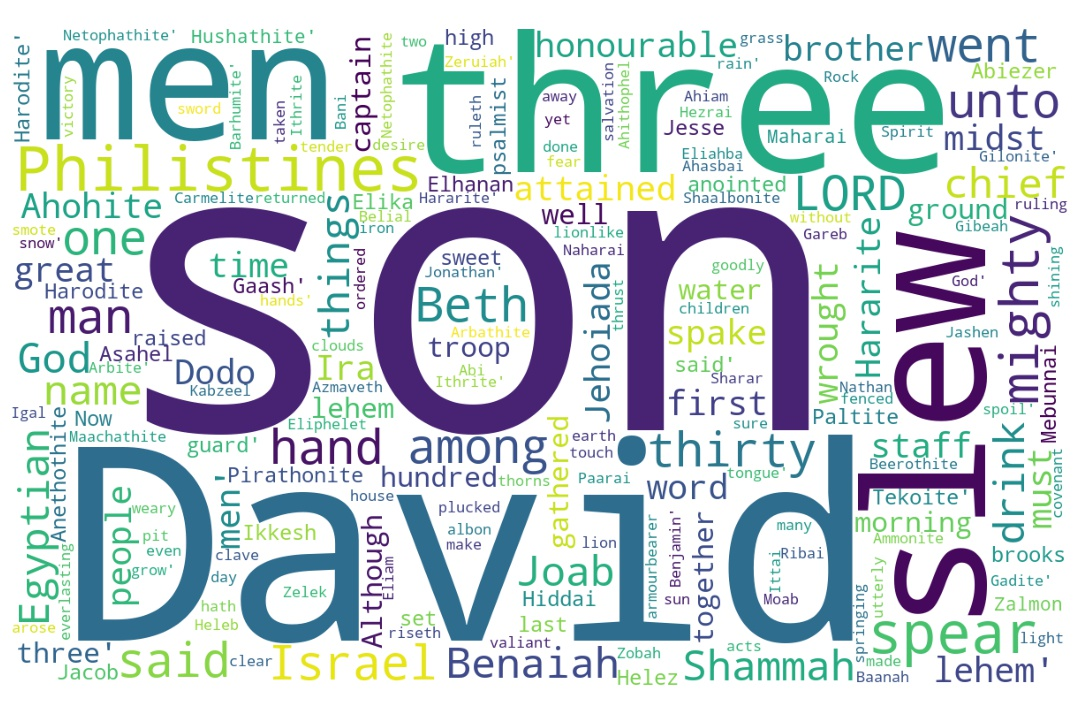
\includegraphics[width=\linewidth]{10OT-2Samuel/2Samuel23-WordCloud.jpg}
  \caption{1 Samuel 23 Word Cloud}
  \label{fig:1 Samuel 23 Word Cloud}
\end{figure}

%%%%%%%%%%%%%%%%%%%%%%%%%%%%%%%%%%%%%%%%%
%%%%%%%%%%%%%%%%%%%%%%%%%%%%%%%%%%%%%%%%%


\marginpar{\scriptsize \centering \fcolorbox{bone}{lime}{\textbf{DAVID"S MIGHTY MEN}}\\ (2 Samuel 23:1--39) 
\begin{compactenum}[I.][8]
    \item A Final  \textbf{Message} \index[scripture]{2Samuel!2Sa 22:01} (2Sa 22:1) 
    \item Things that are  \textbf{Memorable} \index[scripture]{2Samuel!2Sa 22:01} (2Sa 22:1) 
    \item The  \textbf{Mighty} Men \index[scripture]{2Samuel!2Sa 22:01} (2Sa 22:1) 
    \item Those Even  \textbf{More} Special \index[scripture]{2Samuel!2Sa 22:01} (2Sa 22:1) 
    \item A  \textbf{Moment} \index[scripture]{2Samuel!2Sa 23:13--17} (2Sa 23:13--17) 
    \item The  \textbf{Mistake} \index[scripture]{2Samuel!2Sa 23:39} (2Sa 23:39) 
   \item A  \textbf{Message} \index[scripture]{2Samuel!2Sa 23:13--17} (2Sa 23:13--17) 
\end{compactenum} }

\footnote{\textcolor[cmyk]{0.99998,1,0,0}{\hyperlink{TOC}{Return to end of Table of Contents.}}}\footnote{\href{https://audiobible.com/bible/2_samuel_23.html}{\textcolor[cmyk]{0.99998,1,0,0}{2 Samuel 23 Audio}}}\textcolor[cmyk]{0.99998,1,0,0}{Now these \emph{be} the last words of David. David the son of Jesse said, and the man \emph{who} \emph{was} raised up on high, the anointed of the God of Jacob, and the sweet psalmist of Israel, said,}
[2] \textcolor[cmyk]{0.99998,1,0,0}{The Spirit of the LORD spake by me, and his word \emph{was} in my tongue.}
[3] \textcolor[cmyk]{0.99998,1,0,0}{The God of Israel said, the Rock of Israel spake to me, He that ruleth over men \emph{must} \emph{be} just, ruling in the fear of God.}
[4] \textcolor[cmyk]{0.99998,1,0,0}{And \emph{he} \emph{shall} \emph{be} as the light of the morning, \emph{when} the sun riseth, \emph{even} \fcolorbox{bone}{bone}{a}morning without clouds; \emph{as} the tender grass \emph{springing} out of the earth by clear shining after rain.}
[5] \textcolor[cmyk]{0.99998,1,0,0}{Although my house \emph{be} not so with God; yet he hath made with me an everlasting covenant, ordered in all \emph{things}, and sure: for \emph{this} \emph{is} all my salvation, and all \emph{my} desire, although he make \emph{it} not to grow.}\\
\\
\P \textcolor[cmyk]{0.99998,1,0,0}{But \emph{the} \emph{sons} of Belial \emph{shall} \emph{be} all of them as thorns thrust away, because they cannot be taken with hands:}
[7] \textcolor[cmyk]{0.99998,1,0,0}{But the man \emph{that} shall touch them must be fenced with iron and the staff of \fcolorbox{bone}{bone}{a}spear; and they shall be utterly burned with fire in the \emph{same} place.}\\
\\
\P \textcolor[cmyk]{0.99998,1,0,0}{These \emph{be} the names of the mighty men whom David had: The Tachmonite that sat in the seat, chief among the captains; the same \emph{was} Adino the Eznite: \emph{he} \emph{lift} \emph{up} \emph{his} \emph{spear} against eight hundred, whom he slew at one time.}
[9] \textcolor[cmyk]{0.99998,1,0,0}{And after him \emph{was} Eleazar the son of Dodo the Ahohite, \emph{one} of the three mighty men with David, when they defied the Philistines \emph{that} were there gathered together to battle, and the men of Israel were gone away:}
[10] \textcolor[cmyk]{0.99998,1,0,0}{He arose, and smote the Philistines until his hand was weary, and his hand clave unto the sword: and the LORD wrought \fcolorbox{bone}{bone}{a}great victory that day; and the people returned after him only to spoil.}
[11] \textcolor[cmyk]{0.99998,1,0,0}{And after him \emph{was} Shammah the son of Agee the Hararite. And the Philistines were gathered together into \fcolorbox{bone}{bone}{a}troop, where was \fcolorbox{bone}{bone}{a}piece of ground full of lentiles: and the people fled from the Philistines.}
[12] \textcolor[cmyk]{0.99998,1,0,0}{But he stood in the midst of the ground, and defended it, and slew the Philistines: and the LORD wrought \fcolorbox{bone}{bone}{a}great victory.}
[13] \textcolor[cmyk]{0.99998,1,0,0}{And three of the thirty chief went down, and came to David in the harvest time unto the cave of Adullam: and the troop of the Philistines pitched in the valley of Rephaim.}
[14] \textcolor[cmyk]{0.99998,1,0,0}{And David \emph{was} then in an hold, and the garrison of the Philistines \emph{was} then \emph{in} Beth-lehem.}
[15] \textcolor[cmyk]{0.99998,1,0,0}{And David longed, and said, Oh that one would give me drink of the water of the well of Beth-lehem, which \emph{is} by the gate!}
[16] \textcolor[cmyk]{0.99998,1,0,0}{And the three mighty men brake through the host of the Philistines, and drew water out of the well of Beth-lehem, that \emph{was} by the gate, and took \emph{it}, and brought \emph{it} to David: nevertheless he would not drink thereof, but poured it out unto the LORD.}
[17] \textcolor[cmyk]{0.99998,1,0,0}{And he said, Be it far from me, O LORD, that I should do this: \emph{is} \emph{not} \emph{this} the blood of the men that went in jeopardy of their lives? therefore he would not drink it. These things did these three mighty men.}
[18] \textcolor[cmyk]{0.99998,1,0,0}{And Abishai, the brother of Joab, the son of Zeruiah, was chief among three. And he lifted up his spear against three hundred, \emph{and} slew \emph{them}, and had the name among three.}
[19] \textcolor[cmyk]{0.99998,1,0,0}{Was he not most honourable of three? therefore he was their captain: howbeit he attained not unto the \emph{first} three.}
[20] \textcolor[cmyk]{0.99998,1,0,0}{And Benaiah the son of Jehoiada, the son of \fcolorbox{bone}{bone}{a}valiant man, of Kabzeel, who had done many acts, he slew two lionlike men of Moab: he went down also and slew \fcolorbox{bone}{bone}{a}lion in the midst of \fcolorbox{bone}{bone}{a}pit in time of snow:}
[21] \textcolor[cmyk]{0.99998,1,0,0}{And he slew an Egyptian, \fcolorbox{bone}{bone}{a}goodly man: and the Egyptian had \fcolorbox{bone}{bone}{a}spear in his hand; but he went down to him with \fcolorbox{bone}{bone}{a}staff, and plucked the spear out of the Egyptian's hand, and slew him with his own spear.}
[22] \textcolor[cmyk]{0.99998,1,0,0}{These \emph{things} did Benaiah the son of Jehoiada, and had the name among three mighty men.}
[23] \textcolor[cmyk]{0.99998,1,0,0}{He was more honourable than the thirty, but he attained not to the \emph{first} three. And David set him over his guard.}
[24] \textcolor[cmyk]{0.99998,1,0,0}{Asahel the brother of Joab \emph{was} one of the thirty; Elhanan the son of Dodo of Beth-lehem,}
[25] \textcolor[cmyk]{0.99998,1,0,0}{Shammah the Harodite, Elika the Harodite,}
[26] \textcolor[cmyk]{0.99998,1,0,0}{Helez the Paltite, Ira the son of Ikkesh the Tekoite,}
[27] \textcolor[cmyk]{0.99998,1,0,0}{Abiezer the Anethothite, Mebunnai the Hushathite,}
[28] \textcolor[cmyk]{0.99998,1,0,0}{Zalmon the Ahohite, Maharai the Netophathite,}
[29] \textcolor[cmyk]{0.99998,1,0,0}{Heleb the son of Baanah, \fcolorbox{bone}{bone}{a}Netophathite, Ittai the son of Ribai out of Gibeah of the children of Benjamin,}
[30] \textcolor[cmyk]{0.99998,1,0,0}{Benaiah the Pirathonite, Hiddai of the brooks of Gaash,}
[31] \textcolor[cmyk]{0.99998,1,0,0}{Abi-albon the Arbathite, Azmaveth the Barhumite,}
[32] \textcolor[cmyk]{0.99998,1,0,0}{Eliahba the Shaalbonite, of the sons of Jashen, Jonathan,}
[33] \textcolor[cmyk]{0.99998,1,0,0}{Shammah the Hararite, Ahiam the son of Sharar the Hararite,}
[34] \textcolor[cmyk]{0.99998,1,0,0}{Eliphelet the son of Ahasbai, the son of the Maachathite, Eliam the son of Ahithophel the Gilonite,}
[35] \textcolor[cmyk]{0.99998,1,0,0}{Hezrai the Carmelite, Paarai the Arbite,}
[36] \textcolor[cmyk]{0.99998,1,0,0}{Igal the son of Nathan of Zobah, Bani the Gadite,}
[37] \textcolor[cmyk]{0.99998,1,0,0}{Zelek the Ammonite, Naharai the Beerothite, armourbearer to Joab the son of Zeruiah,}
[38] \textcolor[cmyk]{0.99998,1,0,0}{Ira an Ithrite, Gareb an Ithrite,}
[39] \textcolor[cmyk]{0.99998,1,0,0}{Uriah the Hittite: thirty and seven in all.}
\index[NWIV]{37!2Samuel!2Sa 23:1}\index[AWIP]{Now!2Samuel!2Sa 23:1}\index[AWIP]{these!2Samuel!2Sa 23:1}\index[AWIP]{\emph{be}!2Samuel!2Sa 23:1}\index[AWIP]{the!2Samuel!2Sa 23:1}\index[AWIP]{the!2Samuel!2Sa 23:1 (2)}\index[AWIP]{the!2Samuel!2Sa 23:1 (3)}\index[AWIP]{the!2Samuel!2Sa 23:1 (4)}\index[AWIP]{the!2Samuel!2Sa 23:1 (5)}\index[AWIP]{the!2Samuel!2Sa 23:1 (6)}\index[AWIP]{last!2Samuel!2Sa 23:1}\index[AWIP]{words!2Samuel!2Sa 23:1}\index[AWIP]{of!2Samuel!2Sa 23:1}\index[AWIP]{of!2Samuel!2Sa 23:1 (2)}\index[AWIP]{of!2Samuel!2Sa 23:1 (3)}\index[AWIP]{of!2Samuel!2Sa 23:1 (4)}\index[AWIP]{of!2Samuel!2Sa 23:1 (5)}\index[AWIP]{David!2Samuel!2Sa 23:1}\index[AWIP]{David!2Samuel!2Sa 23:1 (2)}\index[AWIP]{son!2Samuel!2Sa 23:1}\index[AWIP]{Jesse!2Samuel!2Sa 23:1}\index[AWIP]{said!2Samuel!2Sa 23:1}\index[AWIP]{said!2Samuel!2Sa 23:1 (2)}\index[AWIP]{and!2Samuel!2Sa 23:1}\index[AWIP]{and!2Samuel!2Sa 23:1 (2)}\index[AWIP]{man!2Samuel!2Sa 23:1}\index[AWIP]{\emph{who}!2Samuel!2Sa 23:1}\index[AWIP]{\emph{was}!2Samuel!2Sa 23:1}\index[AWIP]{raised!2Samuel!2Sa 23:1}\index[AWIP]{up!2Samuel!2Sa 23:1}\index[AWIP]{on!2Samuel!2Sa 23:1}\index[AWIP]{high!2Samuel!2Sa 23:1}\index[AWIP]{anointed!2Samuel!2Sa 23:1}\index[AWIP]{God!2Samuel!2Sa 23:1}\index[AWIP]{Jacob!2Samuel!2Sa 23:1}\index[AWIP]{sweet!2Samuel!2Sa 23:1}\index[AWIP]{psalmist!2Samuel!2Sa 23:1}\index[AWIP]{Israel!2Samuel!2Sa 23:1}\index[AWIP]{\emph{be}!2Samuel!2Sa 23:1}\index[AWIP]{\emph{who}!2Samuel!2Sa 23:1}\index[AWIP]{\emph{was}!2Samuel!2Sa 23:1}

\index[NWIV]{15!2Samuel!2Sa 23:2}\index[AWIP]{The!2Samuel!2Sa 23:2}\index[AWIP]{Spirit!2Samuel!2Sa 23:2}\index[AWIP]{of!2Samuel!2Sa 23:2}\index[AWIP]{the!2Samuel!2Sa 23:2}\index[AWIP]{LORD!2Samuel!2Sa 23:2}\index[AWIP]{spake!2Samuel!2Sa 23:2}\index[AWIP]{by!2Samuel!2Sa 23:2}\index[AWIP]{me!2Samuel!2Sa 23:2}\index[AWIP]{and!2Samuel!2Sa 23:2}\index[AWIP]{his!2Samuel!2Sa 23:2}\index[AWIP]{word!2Samuel!2Sa 23:2}\index[AWIP]{\emph{was}!2Samuel!2Sa 23:2}\index[AWIP]{in!2Samuel!2Sa 23:2}\index[AWIP]{my!2Samuel!2Sa 23:2}\index[AWIP]{tongue!2Samuel!2Sa 23:2}\index[AWIP]{\emph{was}!2Samuel!2Sa 23:2}

\index[NWIV]{26!2Samuel!2Sa 23:3}\index[AWIP]{The!2Samuel!2Sa 23:3}\index[AWIP]{God!2Samuel!2Sa 23:3}\index[AWIP]{God!2Samuel!2Sa 23:3 (2)}\index[AWIP]{of!2Samuel!2Sa 23:3}\index[AWIP]{of!2Samuel!2Sa 23:3 (2)}\index[AWIP]{of!2Samuel!2Sa 23:3 (3)}\index[AWIP]{Israel!2Samuel!2Sa 23:3}\index[AWIP]{Israel!2Samuel!2Sa 23:3 (2)}\index[AWIP]{said!2Samuel!2Sa 23:3}\index[AWIP]{the!2Samuel!2Sa 23:3}\index[AWIP]{the!2Samuel!2Sa 23:3 (2)}\index[AWIP]{Rock!2Samuel!2Sa 23:3}\index[AWIP]{spake!2Samuel!2Sa 23:3}\index[AWIP]{to!2Samuel!2Sa 23:3}\index[AWIP]{me!2Samuel!2Sa 23:3}\index[AWIP]{He!2Samuel!2Sa 23:3}\index[AWIP]{that!2Samuel!2Sa 23:3}\index[AWIP]{ruleth!2Samuel!2Sa 23:3}\index[AWIP]{over!2Samuel!2Sa 23:3}\index[AWIP]{men!2Samuel!2Sa 23:3}\index[AWIP]{\emph{must}!2Samuel!2Sa 23:3}\index[AWIP]{\emph{be}!2Samuel!2Sa 23:3}\index[AWIP]{just!2Samuel!2Sa 23:3}\index[AWIP]{ruling!2Samuel!2Sa 23:3}\index[AWIP]{in!2Samuel!2Sa 23:3}\index[AWIP]{fear!2Samuel!2Sa 23:3}\index[AWIP]{\emph{must}!2Samuel!2Sa 23:3}\index[AWIP]{\emph{be}!2Samuel!2Sa 23:3}

\index[NWIV]{33!2Samuel!2Sa 23:4}\index[AWIP]{And!2Samuel!2Sa 23:4}\index[AWIP]{\emph{he}!2Samuel!2Sa 23:4}\index[AWIP]{\emph{shall}!2Samuel!2Sa 23:4}\index[AWIP]{\emph{be}!2Samuel!2Sa 23:4}\index[AWIP]{as!2Samuel!2Sa 23:4}\index[AWIP]{the!2Samuel!2Sa 23:4}\index[AWIP]{the!2Samuel!2Sa 23:4 (2)}\index[AWIP]{the!2Samuel!2Sa 23:4 (3)}\index[AWIP]{the!2Samuel!2Sa 23:4 (4)}\index[AWIP]{the!2Samuel!2Sa 23:4 (5)}\index[AWIP]{light!2Samuel!2Sa 23:4}\index[AWIP]{of!2Samuel!2Sa 23:4}\index[AWIP]{of!2Samuel!2Sa 23:4 (2)}\index[AWIP]{morning!2Samuel!2Sa 23:4}\index[AWIP]{morning!2Samuel!2Sa 23:4 (2)}\index[AWIP]{\emph{when}!2Samuel!2Sa 23:4}\index[AWIP]{sun!2Samuel!2Sa 23:4}\index[AWIP]{riseth!2Samuel!2Sa 23:4}\index[AWIP]{\emph{even}!2Samuel!2Sa 23:4}\index[AWIP]{a!2Samuel!2Sa 23:4}\index[AWIP]{without!2Samuel!2Sa 23:4}\index[AWIP]{clouds!2Samuel!2Sa 23:4}\index[AWIP]{\emph{as}!2Samuel!2Sa 23:4}\index[AWIP]{tender!2Samuel!2Sa 23:4}\index[AWIP]{grass!2Samuel!2Sa 23:4}\index[AWIP]{\emph{springing}!2Samuel!2Sa 23:4}\index[AWIP]{out!2Samuel!2Sa 23:4}\index[AWIP]{earth!2Samuel!2Sa 23:4}\index[AWIP]{by!2Samuel!2Sa 23:4}\index[AWIP]{clear!2Samuel!2Sa 23:4}\index[AWIP]{shining!2Samuel!2Sa 23:4}\index[AWIP]{after!2Samuel!2Sa 23:4}\index[AWIP]{rain!2Samuel!2Sa 23:4}\index[AWIP]{\emph{he}!2Samuel!2Sa 23:4}\index[AWIP]{\emph{shall}!2Samuel!2Sa 23:4}\index[AWIP]{\emph{be}!2Samuel!2Sa 23:4}\index[AWIP]{\emph{when}!2Samuel!2Sa 23:4}\index[AWIP]{\emph{even}!2Samuel!2Sa 23:4}\index[AWIP]{\emph{as}!2Samuel!2Sa 23:4}\index[AWIP]{\emph{springing}!2Samuel!2Sa 23:4}

\index[NWIV]{40!2Samuel!2Sa 23:5}\index[AWIP]{Although!2Samuel!2Sa 23:5}\index[AWIP]{my!2Samuel!2Sa 23:5}\index[AWIP]{my!2Samuel!2Sa 23:5 (2)}\index[AWIP]{house!2Samuel!2Sa 23:5}\index[AWIP]{\emph{be}!2Samuel!2Sa 23:5}\index[AWIP]{not!2Samuel!2Sa 23:5}\index[AWIP]{not!2Samuel!2Sa 23:5 (2)}\index[AWIP]{so!2Samuel!2Sa 23:5}\index[AWIP]{with!2Samuel!2Sa 23:5}\index[AWIP]{with!2Samuel!2Sa 23:5 (2)}\index[AWIP]{God!2Samuel!2Sa 23:5}\index[AWIP]{yet!2Samuel!2Sa 23:5}\index[AWIP]{he!2Samuel!2Sa 23:5}\index[AWIP]{he!2Samuel!2Sa 23:5 (2)}\index[AWIP]{hath!2Samuel!2Sa 23:5}\index[AWIP]{made!2Samuel!2Sa 23:5}\index[AWIP]{me!2Samuel!2Sa 23:5}\index[AWIP]{an!2Samuel!2Sa 23:5}\index[AWIP]{everlasting!2Samuel!2Sa 23:5}\index[AWIP]{covenant!2Samuel!2Sa 23:5}\index[AWIP]{ordered!2Samuel!2Sa 23:5}\index[AWIP]{in!2Samuel!2Sa 23:5}\index[AWIP]{all!2Samuel!2Sa 23:5}\index[AWIP]{all!2Samuel!2Sa 23:5 (2)}\index[AWIP]{all!2Samuel!2Sa 23:5 (3)}\index[AWIP]{\emph{things}!2Samuel!2Sa 23:5}\index[AWIP]{and!2Samuel!2Sa 23:5}\index[AWIP]{and!2Samuel!2Sa 23:5 (2)}\index[AWIP]{sure!2Samuel!2Sa 23:5}\index[AWIP]{for!2Samuel!2Sa 23:5}\index[AWIP]{\emph{this}!2Samuel!2Sa 23:5}\index[AWIP]{\emph{is}!2Samuel!2Sa 23:5}\index[AWIP]{salvation!2Samuel!2Sa 23:5}\index[AWIP]{\emph{my}!2Samuel!2Sa 23:5}\index[AWIP]{desire!2Samuel!2Sa 23:5}\index[AWIP]{although!2Samuel!2Sa 23:5}\index[AWIP]{make!2Samuel!2Sa 23:5}\index[AWIP]{\emph{it}!2Samuel!2Sa 23:5}\index[AWIP]{to!2Samuel!2Sa 23:5}\index[AWIP]{grow!2Samuel!2Sa 23:5}\index[AWIP]{\emph{be}!2Samuel!2Sa 23:5}\index[AWIP]{\emph{things}!2Samuel!2Sa 23:5}\index[AWIP]{\emph{this}!2Samuel!2Sa 23:5}\index[AWIP]{\emph{is}!2Samuel!2Sa 23:5}\index[AWIP]{\emph{my}!2Samuel!2Sa 23:5}\index[AWIP]{\emph{it}!2Samuel!2Sa 23:5}

\index[NWIV]{21!2Samuel!2Sa 23:6}\index[AWIP]{But!2Samuel!2Sa 23:6}\index[AWIP]{\emph{the}!2Samuel!2Sa 23:6}\index[AWIP]{\emph{sons}!2Samuel!2Sa 23:6}\index[AWIP]{of!2Samuel!2Sa 23:6}\index[AWIP]{of!2Samuel!2Sa 23:6 (2)}\index[AWIP]{Belial!2Samuel!2Sa 23:6}\index[AWIP]{\emph{shall}!2Samuel!2Sa 23:6}\index[AWIP]{\emph{be}!2Samuel!2Sa 23:6}\index[AWIP]{all!2Samuel!2Sa 23:6}\index[AWIP]{them!2Samuel!2Sa 23:6}\index[AWIP]{as!2Samuel!2Sa 23:6}\index[AWIP]{thorns!2Samuel!2Sa 23:6}\index[AWIP]{thrust!2Samuel!2Sa 23:6}\index[AWIP]{away!2Samuel!2Sa 23:6}\index[AWIP]{because!2Samuel!2Sa 23:6}\index[AWIP]{they!2Samuel!2Sa 23:6}\index[AWIP]{cannot!2Samuel!2Sa 23:6}\index[AWIP]{be!2Samuel!2Sa 23:6}\index[AWIP]{taken!2Samuel!2Sa 23:6}\index[AWIP]{with!2Samuel!2Sa 23:6}\index[AWIP]{hands!2Samuel!2Sa 23:6}\index[AWIP]{\emph{the}!2Samuel!2Sa 23:6}\index[AWIP]{\emph{sons}!2Samuel!2Sa 23:6}\index[AWIP]{\emph{shall}!2Samuel!2Sa 23:6}\index[AWIP]{\emph{be}!2Samuel!2Sa 23:6}

\index[NWIV]{30!2Samuel!2Sa 23:7}\index[AWIP]{But!2Samuel!2Sa 23:7}\index[AWIP]{the!2Samuel!2Sa 23:7}\index[AWIP]{the!2Samuel!2Sa 23:7 (2)}\index[AWIP]{the!2Samuel!2Sa 23:7 (3)}\index[AWIP]{man!2Samuel!2Sa 23:7}\index[AWIP]{\emph{that}!2Samuel!2Sa 23:7}\index[AWIP]{shall!2Samuel!2Sa 23:7}\index[AWIP]{shall!2Samuel!2Sa 23:7 (2)}\index[AWIP]{touch!2Samuel!2Sa 23:7}\index[AWIP]{them!2Samuel!2Sa 23:7}\index[AWIP]{must!2Samuel!2Sa 23:7}\index[AWIP]{be!2Samuel!2Sa 23:7}\index[AWIP]{be!2Samuel!2Sa 23:7 (2)}\index[AWIP]{fenced!2Samuel!2Sa 23:7}\index[AWIP]{with!2Samuel!2Sa 23:7}\index[AWIP]{with!2Samuel!2Sa 23:7 (2)}\index[AWIP]{iron!2Samuel!2Sa 23:7}\index[AWIP]{and!2Samuel!2Sa 23:7}\index[AWIP]{and!2Samuel!2Sa 23:7 (2)}\index[AWIP]{staff!2Samuel!2Sa 23:7}\index[AWIP]{of!2Samuel!2Sa 23:7}\index[AWIP]{a!2Samuel!2Sa 23:7}\index[AWIP]{spear!2Samuel!2Sa 23:7}\index[AWIP]{they!2Samuel!2Sa 23:7}\index[AWIP]{utterly!2Samuel!2Sa 23:7}\index[AWIP]{burned!2Samuel!2Sa 23:7}\index[AWIP]{fire!2Samuel!2Sa 23:7}\index[AWIP]{in!2Samuel!2Sa 23:7}\index[AWIP]{\emph{same}!2Samuel!2Sa 23:7}\index[AWIP]{place!2Samuel!2Sa 23:7}\index[AWIP]{\emph{that}!2Samuel!2Sa 23:7}\index[AWIP]{\emph{same}!2Samuel!2Sa 23:7}

\index[NWIV]{42!2Samuel!2Sa 23:8}\index[AWIP]{These!2Samuel!2Sa 23:8}\index[AWIP]{\emph{be}!2Samuel!2Sa 23:8}\index[AWIP]{the!2Samuel!2Sa 23:8}\index[AWIP]{the!2Samuel!2Sa 23:8 (2)}\index[AWIP]{the!2Samuel!2Sa 23:8 (3)}\index[AWIP]{the!2Samuel!2Sa 23:8 (4)}\index[AWIP]{the!2Samuel!2Sa 23:8 (5)}\index[AWIP]{the!2Samuel!2Sa 23:8 (6)}\index[AWIP]{names!2Samuel!2Sa 23:8}\index[AWIP]{of!2Samuel!2Sa 23:8}\index[AWIP]{mighty!2Samuel!2Sa 23:8}\index[AWIP]{men!2Samuel!2Sa 23:8}\index[AWIP]{whom!2Samuel!2Sa 23:8}\index[AWIP]{whom!2Samuel!2Sa 23:8 (2)}\index[AWIP]{David!2Samuel!2Sa 23:8}\index[AWIP]{had!2Samuel!2Sa 23:8}\index[AWIP]{The!2Samuel!2Sa 23:8}\index[AWIP]{Tachmonite!2Samuel!2Sa 23:8}\index[AWIP]{that!2Samuel!2Sa 23:8}\index[AWIP]{sat!2Samuel!2Sa 23:8}\index[AWIP]{in!2Samuel!2Sa 23:8}\index[AWIP]{seat!2Samuel!2Sa 23:8}\index[AWIP]{chief!2Samuel!2Sa 23:8}\index[AWIP]{among!2Samuel!2Sa 23:8}\index[AWIP]{captains!2Samuel!2Sa 23:8}\index[AWIP]{same!2Samuel!2Sa 23:8}\index[AWIP]{\emph{was}!2Samuel!2Sa 23:8}\index[AWIP]{Adino!2Samuel!2Sa 23:8}\index[AWIP]{Eznite!2Samuel!2Sa 23:8}\index[AWIP]{\emph{he}!2Samuel!2Sa 23:8}\index[AWIP]{\emph{lift}!2Samuel!2Sa 23:8}\index[AWIP]{\emph{up}!2Samuel!2Sa 23:8}\index[AWIP]{\emph{his}!2Samuel!2Sa 23:8}\index[AWIP]{\emph{spear}!2Samuel!2Sa 23:8}\index[AWIP]{against!2Samuel!2Sa 23:8}\index[AWIP]{eight!2Samuel!2Sa 23:8}\index[AWIP]{hundred!2Samuel!2Sa 23:8}\index[AWIP]{he!2Samuel!2Sa 23:8}\index[AWIP]{slew!2Samuel!2Sa 23:8}\index[AWIP]{at!2Samuel!2Sa 23:8}\index[AWIP]{one!2Samuel!2Sa 23:8}\index[AWIP]{time!2Samuel!2Sa 23:8}\index[AWIP]{\emph{be}!2Samuel!2Sa 23:8}\index[AWIP]{\emph{was}!2Samuel!2Sa 23:8}\index[AWIP]{\emph{he}!2Samuel!2Sa 23:8}\index[AWIP]{\emph{lift}!2Samuel!2Sa 23:8}\index[AWIP]{\emph{up}!2Samuel!2Sa 23:8}\index[AWIP]{\emph{his}!2Samuel!2Sa 23:8}\index[AWIP]{\emph{spear}!2Samuel!2Sa 23:8}

\index[NWIV]{39!2Samuel!2Sa 23:9}\index[AWIP]{And!2Samuel!2Sa 23:9}\index[AWIP]{after!2Samuel!2Sa 23:9}\index[AWIP]{him!2Samuel!2Sa 23:9}\index[AWIP]{\emph{was}!2Samuel!2Sa 23:9}\index[AWIP]{Eleazar!2Samuel!2Sa 23:9}\index[AWIP]{the!2Samuel!2Sa 23:9}\index[AWIP]{the!2Samuel!2Sa 23:9 (2)}\index[AWIP]{the!2Samuel!2Sa 23:9 (3)}\index[AWIP]{the!2Samuel!2Sa 23:9 (4)}\index[AWIP]{the!2Samuel!2Sa 23:9 (5)}\index[AWIP]{son!2Samuel!2Sa 23:9}\index[AWIP]{of!2Samuel!2Sa 23:9}\index[AWIP]{of!2Samuel!2Sa 23:9 (2)}\index[AWIP]{of!2Samuel!2Sa 23:9 (3)}\index[AWIP]{Dodo!2Samuel!2Sa 23:9}\index[AWIP]{Ahohite!2Samuel!2Sa 23:9}\index[AWIP]{\emph{one}!2Samuel!2Sa 23:9}\index[AWIP]{three!2Samuel!2Sa 23:9}\index[AWIP]{mighty!2Samuel!2Sa 23:9}\index[AWIP]{men!2Samuel!2Sa 23:9}\index[AWIP]{men!2Samuel!2Sa 23:9 (2)}\index[AWIP]{with!2Samuel!2Sa 23:9}\index[AWIP]{David!2Samuel!2Sa 23:9}\index[AWIP]{when!2Samuel!2Sa 23:9}\index[AWIP]{they!2Samuel!2Sa 23:9}\index[AWIP]{defied!2Samuel!2Sa 23:9}\index[AWIP]{Philistines!2Samuel!2Sa 23:9}\index[AWIP]{\emph{that}!2Samuel!2Sa 23:9}\index[AWIP]{were!2Samuel!2Sa 23:9}\index[AWIP]{were!2Samuel!2Sa 23:9 (2)}\index[AWIP]{there!2Samuel!2Sa 23:9}\index[AWIP]{gathered!2Samuel!2Sa 23:9}\index[AWIP]{together!2Samuel!2Sa 23:9}\index[AWIP]{to!2Samuel!2Sa 23:9}\index[AWIP]{battle!2Samuel!2Sa 23:9}\index[AWIP]{and!2Samuel!2Sa 23:9}\index[AWIP]{Israel!2Samuel!2Sa 23:9}\index[AWIP]{gone!2Samuel!2Sa 23:9}\index[AWIP]{away!2Samuel!2Sa 23:9}\index[AWIP]{\emph{was}!2Samuel!2Sa 23:9}\index[AWIP]{\emph{one}!2Samuel!2Sa 23:9}\index[AWIP]{\emph{that}!2Samuel!2Sa 23:9}

\index[NWIV]{36!2Samuel!2Sa 23:10}\index[AWIP]{He!2Samuel!2Sa 23:10}\index[AWIP]{arose!2Samuel!2Sa 23:10}\index[AWIP]{and!2Samuel!2Sa 23:10}\index[AWIP]{and!2Samuel!2Sa 23:10 (2)}\index[AWIP]{and!2Samuel!2Sa 23:10 (3)}\index[AWIP]{and!2Samuel!2Sa 23:10 (4)}\index[AWIP]{smote!2Samuel!2Sa 23:10}\index[AWIP]{the!2Samuel!2Sa 23:10}\index[AWIP]{the!2Samuel!2Sa 23:10 (2)}\index[AWIP]{the!2Samuel!2Sa 23:10 (3)}\index[AWIP]{the!2Samuel!2Sa 23:10 (4)}\index[AWIP]{Philistines!2Samuel!2Sa 23:10}\index[AWIP]{until!2Samuel!2Sa 23:10}\index[AWIP]{his!2Samuel!2Sa 23:10}\index[AWIP]{his!2Samuel!2Sa 23:10 (2)}\index[AWIP]{hand!2Samuel!2Sa 23:10}\index[AWIP]{hand!2Samuel!2Sa 23:10 (2)}\index[AWIP]{was!2Samuel!2Sa 23:10}\index[AWIP]{weary!2Samuel!2Sa 23:10}\index[AWIP]{clave!2Samuel!2Sa 23:10}\index[AWIP]{unto!2Samuel!2Sa 23:10}\index[AWIP]{sword!2Samuel!2Sa 23:10}\index[AWIP]{LORD!2Samuel!2Sa 23:10}\index[AWIP]{wrought!2Samuel!2Sa 23:10}\index[AWIP]{a!2Samuel!2Sa 23:10}\index[AWIP]{great!2Samuel!2Sa 23:10}\index[AWIP]{victory!2Samuel!2Sa 23:10}\index[AWIP]{that!2Samuel!2Sa 23:10}\index[AWIP]{day!2Samuel!2Sa 23:10}\index[AWIP]{people!2Samuel!2Sa 23:10}\index[AWIP]{returned!2Samuel!2Sa 23:10}\index[AWIP]{after!2Samuel!2Sa 23:10}\index[AWIP]{him!2Samuel!2Sa 23:10}\index[AWIP]{only!2Samuel!2Sa 23:10}\index[AWIP]{to!2Samuel!2Sa 23:10}\index[AWIP]{spoil!2Samuel!2Sa 23:10}

\index[NWIV]{36!2Samuel!2Sa 23:11}\index[AWIP]{And!2Samuel!2Sa 23:11}\index[AWIP]{And!2Samuel!2Sa 23:11 (2)}\index[AWIP]{after!2Samuel!2Sa 23:11}\index[AWIP]{him!2Samuel!2Sa 23:11}\index[AWIP]{\emph{was}!2Samuel!2Sa 23:11}\index[AWIP]{Shammah!2Samuel!2Sa 23:11}\index[AWIP]{the!2Samuel!2Sa 23:11}\index[AWIP]{the!2Samuel!2Sa 23:11 (2)}\index[AWIP]{the!2Samuel!2Sa 23:11 (3)}\index[AWIP]{the!2Samuel!2Sa 23:11 (4)}\index[AWIP]{the!2Samuel!2Sa 23:11 (5)}\index[AWIP]{son!2Samuel!2Sa 23:11}\index[AWIP]{of!2Samuel!2Sa 23:11}\index[AWIP]{of!2Samuel!2Sa 23:11 (2)}\index[AWIP]{of!2Samuel!2Sa 23:11 (3)}\index[AWIP]{Agee!2Samuel!2Sa 23:11}\index[AWIP]{Hararite!2Samuel!2Sa 23:11}\index[AWIP]{Philistines!2Samuel!2Sa 23:11}\index[AWIP]{Philistines!2Samuel!2Sa 23:11 (2)}\index[AWIP]{were!2Samuel!2Sa 23:11}\index[AWIP]{gathered!2Samuel!2Sa 23:11}\index[AWIP]{together!2Samuel!2Sa 23:11}\index[AWIP]{into!2Samuel!2Sa 23:11}\index[AWIP]{a!2Samuel!2Sa 23:11}\index[AWIP]{a!2Samuel!2Sa 23:11 (2)}\index[AWIP]{troop!2Samuel!2Sa 23:11}\index[AWIP]{where!2Samuel!2Sa 23:11}\index[AWIP]{was!2Samuel!2Sa 23:11}\index[AWIP]{piece!2Samuel!2Sa 23:11}\index[AWIP]{ground!2Samuel!2Sa 23:11}\index[AWIP]{full!2Samuel!2Sa 23:11}\index[AWIP]{lentiles!2Samuel!2Sa 23:11}\index[AWIP]{and!2Samuel!2Sa 23:11}\index[AWIP]{people!2Samuel!2Sa 23:11}\index[AWIP]{fled!2Samuel!2Sa 23:11}\index[AWIP]{from!2Samuel!2Sa 23:11}\index[AWIP]{\emph{was}!2Samuel!2Sa 23:11}

\index[NWIV]{23!2Samuel!2Sa 23:12}\index[AWIP]{But!2Samuel!2Sa 23:12}\index[AWIP]{he!2Samuel!2Sa 23:12}\index[AWIP]{stood!2Samuel!2Sa 23:12}\index[AWIP]{in!2Samuel!2Sa 23:12}\index[AWIP]{the!2Samuel!2Sa 23:12}\index[AWIP]{the!2Samuel!2Sa 23:12 (2)}\index[AWIP]{the!2Samuel!2Sa 23:12 (3)}\index[AWIP]{the!2Samuel!2Sa 23:12 (4)}\index[AWIP]{midst!2Samuel!2Sa 23:12}\index[AWIP]{of!2Samuel!2Sa 23:12}\index[AWIP]{ground!2Samuel!2Sa 23:12}\index[AWIP]{and!2Samuel!2Sa 23:12}\index[AWIP]{and!2Samuel!2Sa 23:12 (2)}\index[AWIP]{and!2Samuel!2Sa 23:12 (3)}\index[AWIP]{defended!2Samuel!2Sa 23:12}\index[AWIP]{it!2Samuel!2Sa 23:12}\index[AWIP]{slew!2Samuel!2Sa 23:12}\index[AWIP]{Philistines!2Samuel!2Sa 23:12}\index[AWIP]{LORD!2Samuel!2Sa 23:12}\index[AWIP]{wrought!2Samuel!2Sa 23:12}\index[AWIP]{a!2Samuel!2Sa 23:12}\index[AWIP]{great!2Samuel!2Sa 23:12}\index[AWIP]{victory!2Samuel!2Sa 23:12}

\index[NWIV]{33!2Samuel!2Sa 23:13}\index[AWIP]{And!2Samuel!2Sa 23:13}\index[AWIP]{three!2Samuel!2Sa 23:13}\index[AWIP]{of!2Samuel!2Sa 23:13}\index[AWIP]{of!2Samuel!2Sa 23:13 (2)}\index[AWIP]{of!2Samuel!2Sa 23:13 (3)}\index[AWIP]{of!2Samuel!2Sa 23:13 (4)}\index[AWIP]{the!2Samuel!2Sa 23:13}\index[AWIP]{the!2Samuel!2Sa 23:13 (2)}\index[AWIP]{the!2Samuel!2Sa 23:13 (3)}\index[AWIP]{the!2Samuel!2Sa 23:13 (4)}\index[AWIP]{the!2Samuel!2Sa 23:13 (5)}\index[AWIP]{the!2Samuel!2Sa 23:13 (6)}\index[AWIP]{thirty!2Samuel!2Sa 23:13}\index[AWIP]{chief!2Samuel!2Sa 23:13}\index[AWIP]{went!2Samuel!2Sa 23:13}\index[AWIP]{down!2Samuel!2Sa 23:13}\index[AWIP]{and!2Samuel!2Sa 23:13}\index[AWIP]{and!2Samuel!2Sa 23:13 (2)}\index[AWIP]{came!2Samuel!2Sa 23:13}\index[AWIP]{to!2Samuel!2Sa 23:13}\index[AWIP]{David!2Samuel!2Sa 23:13}\index[AWIP]{in!2Samuel!2Sa 23:13}\index[AWIP]{in!2Samuel!2Sa 23:13 (2)}\index[AWIP]{harvest!2Samuel!2Sa 23:13}\index[AWIP]{time!2Samuel!2Sa 23:13}\index[AWIP]{unto!2Samuel!2Sa 23:13}\index[AWIP]{cave!2Samuel!2Sa 23:13}\index[AWIP]{Adullam!2Samuel!2Sa 23:13}\index[AWIP]{troop!2Samuel!2Sa 23:13}\index[AWIP]{Philistines!2Samuel!2Sa 23:13}\index[AWIP]{pitched!2Samuel!2Sa 23:13}\index[AWIP]{valley!2Samuel!2Sa 23:13}\index[AWIP]{Rephaim!2Samuel!2Sa 23:13}

\index[NWIV]{17!2Samuel!2Sa 23:14}\index[AWIP]{And!2Samuel!2Sa 23:14}\index[AWIP]{David!2Samuel!2Sa 23:14}\index[AWIP]{\emph{was}!2Samuel!2Sa 23:14}\index[AWIP]{\emph{was}!2Samuel!2Sa 23:14 (2)}\index[AWIP]{then!2Samuel!2Sa 23:14}\index[AWIP]{then!2Samuel!2Sa 23:14 (2)}\index[AWIP]{in!2Samuel!2Sa 23:14}\index[AWIP]{an!2Samuel!2Sa 23:14}\index[AWIP]{hold!2Samuel!2Sa 23:14}\index[AWIP]{and!2Samuel!2Sa 23:14}\index[AWIP]{the!2Samuel!2Sa 23:14}\index[AWIP]{the!2Samuel!2Sa 23:14 (2)}\index[AWIP]{garrison!2Samuel!2Sa 23:14}\index[AWIP]{of!2Samuel!2Sa 23:14}\index[AWIP]{Philistines!2Samuel!2Sa 23:14}\index[AWIP]{\emph{in}!2Samuel!2Sa 23:14}\index[AWIP]{Beth-lehem!2Samuel!2Sa 23:14}\index[AWIP]{\emph{was}!2Samuel!2Sa 23:14}\index[AWIP]{\emph{was}!2Samuel!2Sa 23:14 (2)}\index[AWIP]{\emph{in}!2Samuel!2Sa 23:14}

\index[NWIV]{25!2Samuel!2Sa 23:15}\index[AWIP]{And!2Samuel!2Sa 23:15}\index[AWIP]{David!2Samuel!2Sa 23:15}\index[AWIP]{longed!2Samuel!2Sa 23:15}\index[AWIP]{and!2Samuel!2Sa 23:15}\index[AWIP]{said!2Samuel!2Sa 23:15}\index[AWIP]{Oh!2Samuel!2Sa 23:15}\index[AWIP]{that!2Samuel!2Sa 23:15}\index[AWIP]{one!2Samuel!2Sa 23:15}\index[AWIP]{would!2Samuel!2Sa 23:15}\index[AWIP]{give!2Samuel!2Sa 23:15}\index[AWIP]{me!2Samuel!2Sa 23:15}\index[AWIP]{drink!2Samuel!2Sa 23:15}\index[AWIP]{of!2Samuel!2Sa 23:15}\index[AWIP]{of!2Samuel!2Sa 23:15 (2)}\index[AWIP]{of!2Samuel!2Sa 23:15 (3)}\index[AWIP]{the!2Samuel!2Sa 23:15}\index[AWIP]{the!2Samuel!2Sa 23:15 (2)}\index[AWIP]{the!2Samuel!2Sa 23:15 (3)}\index[AWIP]{water!2Samuel!2Sa 23:15}\index[AWIP]{well!2Samuel!2Sa 23:15}\index[AWIP]{Beth-lehem!2Samuel!2Sa 23:15}\index[AWIP]{which!2Samuel!2Sa 23:15}\index[AWIP]{\emph{is}!2Samuel!2Sa 23:15}\index[AWIP]{by!2Samuel!2Sa 23:15}\index[AWIP]{gate!!2Samuel!2Sa 23:15}\index[AWIP]{\emph{is}!2Samuel!2Sa 23:15}

\index[NWIV]{47!2Samuel!2Sa 23:16}\index[AWIP]{And!2Samuel!2Sa 23:16}\index[AWIP]{the!2Samuel!2Sa 23:16}\index[AWIP]{the!2Samuel!2Sa 23:16 (2)}\index[AWIP]{the!2Samuel!2Sa 23:16 (3)}\index[AWIP]{the!2Samuel!2Sa 23:16 (4)}\index[AWIP]{the!2Samuel!2Sa 23:16 (5)}\index[AWIP]{the!2Samuel!2Sa 23:16 (6)}\index[AWIP]{three!2Samuel!2Sa 23:16}\index[AWIP]{mighty!2Samuel!2Sa 23:16}\index[AWIP]{men!2Samuel!2Sa 23:16}\index[AWIP]{brake!2Samuel!2Sa 23:16}\index[AWIP]{through!2Samuel!2Sa 23:16}\index[AWIP]{host!2Samuel!2Sa 23:16}\index[AWIP]{of!2Samuel!2Sa 23:16}\index[AWIP]{of!2Samuel!2Sa 23:16 (2)}\index[AWIP]{of!2Samuel!2Sa 23:16 (3)}\index[AWIP]{Philistines!2Samuel!2Sa 23:16}\index[AWIP]{and!2Samuel!2Sa 23:16}\index[AWIP]{and!2Samuel!2Sa 23:16 (2)}\index[AWIP]{and!2Samuel!2Sa 23:16 (3)}\index[AWIP]{drew!2Samuel!2Sa 23:16}\index[AWIP]{water!2Samuel!2Sa 23:16}\index[AWIP]{out!2Samuel!2Sa 23:16}\index[AWIP]{out!2Samuel!2Sa 23:16 (2)}\index[AWIP]{well!2Samuel!2Sa 23:16}\index[AWIP]{Beth-lehem!2Samuel!2Sa 23:16}\index[AWIP]{that!2Samuel!2Sa 23:16}\index[AWIP]{\emph{was}!2Samuel!2Sa 23:16}\index[AWIP]{by!2Samuel!2Sa 23:16}\index[AWIP]{gate!2Samuel!2Sa 23:16}\index[AWIP]{took!2Samuel!2Sa 23:16}\index[AWIP]{\emph{it}!2Samuel!2Sa 23:16}\index[AWIP]{\emph{it}!2Samuel!2Sa 23:16 (2)}\index[AWIP]{brought!2Samuel!2Sa 23:16}\index[AWIP]{to!2Samuel!2Sa 23:16}\index[AWIP]{David!2Samuel!2Sa 23:16}\index[AWIP]{nevertheless!2Samuel!2Sa 23:16}\index[AWIP]{he!2Samuel!2Sa 23:16}\index[AWIP]{would!2Samuel!2Sa 23:16}\index[AWIP]{not!2Samuel!2Sa 23:16}\index[AWIP]{drink!2Samuel!2Sa 23:16}\index[AWIP]{thereof!2Samuel!2Sa 23:16}\index[AWIP]{but!2Samuel!2Sa 23:16}\index[AWIP]{poured!2Samuel!2Sa 23:16}\index[AWIP]{it!2Samuel!2Sa 23:16}\index[AWIP]{unto!2Samuel!2Sa 23:16}\index[AWIP]{LORD!2Samuel!2Sa 23:16}\index[AWIP]{\emph{was}!2Samuel!2Sa 23:16}\index[AWIP]{\emph{it}!2Samuel!2Sa 23:16}\index[AWIP]{\emph{it}!2Samuel!2Sa 23:16 (2)}

\index[NWIV]{43!2Samuel!2Sa 23:17}\index[AWIP]{And!2Samuel!2Sa 23:17}\index[AWIP]{he!2Samuel!2Sa 23:17}\index[AWIP]{he!2Samuel!2Sa 23:17 (2)}\index[AWIP]{said!2Samuel!2Sa 23:17}\index[AWIP]{Be!2Samuel!2Sa 23:17}\index[AWIP]{it!2Samuel!2Sa 23:17}\index[AWIP]{it!2Samuel!2Sa 23:17 (2)}\index[AWIP]{far!2Samuel!2Sa 23:17}\index[AWIP]{from!2Samuel!2Sa 23:17}\index[AWIP]{me!2Samuel!2Sa 23:17}\index[AWIP]{O!2Samuel!2Sa 23:17}\index[AWIP]{LORD!2Samuel!2Sa 23:17}\index[AWIP]{that!2Samuel!2Sa 23:17}\index[AWIP]{that!2Samuel!2Sa 23:17 (2)}\index[AWIP]{I!2Samuel!2Sa 23:17}\index[AWIP]{should!2Samuel!2Sa 23:17}\index[AWIP]{do!2Samuel!2Sa 23:17}\index[AWIP]{this!2Samuel!2Sa 23:17}\index[AWIP]{\emph{is}!2Samuel!2Sa 23:17}\index[AWIP]{\emph{not}!2Samuel!2Sa 23:17}\index[AWIP]{\emph{this}!2Samuel!2Sa 23:17}\index[AWIP]{the!2Samuel!2Sa 23:17}\index[AWIP]{the!2Samuel!2Sa 23:17 (2)}\index[AWIP]{blood!2Samuel!2Sa 23:17}\index[AWIP]{of!2Samuel!2Sa 23:17}\index[AWIP]{of!2Samuel!2Sa 23:17 (2)}\index[AWIP]{men!2Samuel!2Sa 23:17}\index[AWIP]{men!2Samuel!2Sa 23:17 (2)}\index[AWIP]{went!2Samuel!2Sa 23:17}\index[AWIP]{in!2Samuel!2Sa 23:17}\index[AWIP]{jeopardy!2Samuel!2Sa 23:17}\index[AWIP]{their!2Samuel!2Sa 23:17}\index[AWIP]{lives?!2Samuel!2Sa 23:17}\index[AWIP]{therefore!2Samuel!2Sa 23:17}\index[AWIP]{would!2Samuel!2Sa 23:17}\index[AWIP]{not!2Samuel!2Sa 23:17}\index[AWIP]{drink!2Samuel!2Sa 23:17}\index[AWIP]{These!2Samuel!2Sa 23:17}\index[AWIP]{things!2Samuel!2Sa 23:17}\index[AWIP]{did!2Samuel!2Sa 23:17}\index[AWIP]{these!2Samuel!2Sa 23:17}\index[AWIP]{three!2Samuel!2Sa 23:17}\index[AWIP]{mighty!2Samuel!2Sa 23:17}\index[AWIP]{\emph{is}!2Samuel!2Sa 23:17}\index[AWIP]{\emph{not}!2Samuel!2Sa 23:17}\index[AWIP]{\emph{this}!2Samuel!2Sa 23:17}

\index[NWIV]{32!2Samuel!2Sa 23:18}\index[AWIP]{And!2Samuel!2Sa 23:18}\index[AWIP]{And!2Samuel!2Sa 23:18 (2)}\index[AWIP]{Abishai!2Samuel!2Sa 23:18}\index[AWIP]{the!2Samuel!2Sa 23:18}\index[AWIP]{the!2Samuel!2Sa 23:18 (2)}\index[AWIP]{the!2Samuel!2Sa 23:18 (3)}\index[AWIP]{brother!2Samuel!2Sa 23:18}\index[AWIP]{of!2Samuel!2Sa 23:18}\index[AWIP]{of!2Samuel!2Sa 23:18 (2)}\index[AWIP]{Joab!2Samuel!2Sa 23:18}\index[AWIP]{son!2Samuel!2Sa 23:18}\index[AWIP]{Zeruiah!2Samuel!2Sa 23:18}\index[AWIP]{was!2Samuel!2Sa 23:18}\index[AWIP]{chief!2Samuel!2Sa 23:18}\index[AWIP]{among!2Samuel!2Sa 23:18}\index[AWIP]{among!2Samuel!2Sa 23:18 (2)}\index[AWIP]{three!2Samuel!2Sa 23:18}\index[AWIP]{three!2Samuel!2Sa 23:18 (2)}\index[AWIP]{three!2Samuel!2Sa 23:18 (3)}\index[AWIP]{he!2Samuel!2Sa 23:18}\index[AWIP]{lifted!2Samuel!2Sa 23:18}\index[AWIP]{up!2Samuel!2Sa 23:18}\index[AWIP]{his!2Samuel!2Sa 23:18}\index[AWIP]{spear!2Samuel!2Sa 23:18}\index[AWIP]{against!2Samuel!2Sa 23:18}\index[AWIP]{hundred!2Samuel!2Sa 23:18}\index[AWIP]{\emph{and}!2Samuel!2Sa 23:18}\index[AWIP]{slew!2Samuel!2Sa 23:18}\index[AWIP]{\emph{them}!2Samuel!2Sa 23:18}\index[AWIP]{and!2Samuel!2Sa 23:18}\index[AWIP]{had!2Samuel!2Sa 23:18}\index[AWIP]{name!2Samuel!2Sa 23:18}\index[AWIP]{\emph{and}!2Samuel!2Sa 23:18}\index[AWIP]{\emph{them}!2Samuel!2Sa 23:18}

\index[NWIV]{20!2Samuel!2Sa 23:19}\index[AWIP]{Was!2Samuel!2Sa 23:19}\index[AWIP]{he!2Samuel!2Sa 23:19}\index[AWIP]{he!2Samuel!2Sa 23:19 (2)}\index[AWIP]{he!2Samuel!2Sa 23:19 (3)}\index[AWIP]{not!2Samuel!2Sa 23:19}\index[AWIP]{not!2Samuel!2Sa 23:19 (2)}\index[AWIP]{most!2Samuel!2Sa 23:19}\index[AWIP]{honourable!2Samuel!2Sa 23:19}\index[AWIP]{of!2Samuel!2Sa 23:19}\index[AWIP]{three?!2Samuel!2Sa 23:19}\index[AWIP]{therefore!2Samuel!2Sa 23:19}\index[AWIP]{was!2Samuel!2Sa 23:19}\index[AWIP]{their!2Samuel!2Sa 23:19}\index[AWIP]{captain!2Samuel!2Sa 23:19}\index[AWIP]{howbeit!2Samuel!2Sa 23:19}\index[AWIP]{attained!2Samuel!2Sa 23:19}\index[AWIP]{unto!2Samuel!2Sa 23:19}\index[AWIP]{the!2Samuel!2Sa 23:19}\index[AWIP]{\emph{first}!2Samuel!2Sa 23:19}\index[AWIP]{three!2Samuel!2Sa 23:19}\index[AWIP]{\emph{first}!2Samuel!2Sa 23:19}

\index[NWIV]{44!2Samuel!2Sa 23:20}\index[AWIP]{And!2Samuel!2Sa 23:20}\index[AWIP]{Benaiah!2Samuel!2Sa 23:20}\index[AWIP]{the!2Samuel!2Sa 23:20}\index[AWIP]{the!2Samuel!2Sa 23:20 (2)}\index[AWIP]{the!2Samuel!2Sa 23:20 (3)}\index[AWIP]{son!2Samuel!2Sa 23:20}\index[AWIP]{son!2Samuel!2Sa 23:20 (2)}\index[AWIP]{of!2Samuel!2Sa 23:20}\index[AWIP]{of!2Samuel!2Sa 23:20 (2)}\index[AWIP]{of!2Samuel!2Sa 23:20 (3)}\index[AWIP]{of!2Samuel!2Sa 23:20 (4)}\index[AWIP]{of!2Samuel!2Sa 23:20 (5)}\index[AWIP]{of!2Samuel!2Sa 23:20 (6)}\index[AWIP]{Jehoiada!2Samuel!2Sa 23:20}\index[AWIP]{a!2Samuel!2Sa 23:20}\index[AWIP]{a!2Samuel!2Sa 23:20 (2)}\index[AWIP]{a!2Samuel!2Sa 23:20 (3)}\index[AWIP]{valiant!2Samuel!2Sa 23:20}\index[AWIP]{man!2Samuel!2Sa 23:20}\index[AWIP]{Kabzeel!2Samuel!2Sa 23:20}\index[AWIP]{who!2Samuel!2Sa 23:20}\index[AWIP]{had!2Samuel!2Sa 23:20}\index[AWIP]{done!2Samuel!2Sa 23:20}\index[AWIP]{many!2Samuel!2Sa 23:20}\index[AWIP]{acts!2Samuel!2Sa 23:20}\index[AWIP]{he!2Samuel!2Sa 23:20}\index[AWIP]{he!2Samuel!2Sa 23:20 (2)}\index[AWIP]{slew!2Samuel!2Sa 23:20}\index[AWIP]{slew!2Samuel!2Sa 23:20 (2)}\index[AWIP]{two!2Samuel!2Sa 23:20}\index[AWIP]{lionlike!2Samuel!2Sa 23:20}\index[AWIP]{men!2Samuel!2Sa 23:20}\index[AWIP]{Moab!2Samuel!2Sa 23:20}\index[AWIP]{went!2Samuel!2Sa 23:20}\index[AWIP]{down!2Samuel!2Sa 23:20}\index[AWIP]{also!2Samuel!2Sa 23:20}\index[AWIP]{and!2Samuel!2Sa 23:20}\index[AWIP]{lion!2Samuel!2Sa 23:20}\index[AWIP]{in!2Samuel!2Sa 23:20}\index[AWIP]{in!2Samuel!2Sa 23:20 (2)}\index[AWIP]{midst!2Samuel!2Sa 23:20}\index[AWIP]{pit!2Samuel!2Sa 23:20}\index[AWIP]{time!2Samuel!2Sa 23:20}\index[AWIP]{snow!2Samuel!2Sa 23:20}

\index[NWIV]{42!2Samuel!2Sa 23:21}\index[AWIP]{And!2Samuel!2Sa 23:21}\index[AWIP]{he!2Samuel!2Sa 23:21}\index[AWIP]{he!2Samuel!2Sa 23:21 (2)}\index[AWIP]{slew!2Samuel!2Sa 23:21}\index[AWIP]{slew!2Samuel!2Sa 23:21 (2)}\index[AWIP]{an!2Samuel!2Sa 23:21}\index[AWIP]{Egyptian!2Samuel!2Sa 23:21}\index[AWIP]{Egyptian!2Samuel!2Sa 23:21 (2)}\index[AWIP]{a!2Samuel!2Sa 23:21}\index[AWIP]{a!2Samuel!2Sa 23:21 (2)}\index[AWIP]{a!2Samuel!2Sa 23:21 (3)}\index[AWIP]{goodly!2Samuel!2Sa 23:21}\index[AWIP]{man!2Samuel!2Sa 23:21}\index[AWIP]{and!2Samuel!2Sa 23:21}\index[AWIP]{and!2Samuel!2Sa 23:21 (2)}\index[AWIP]{and!2Samuel!2Sa 23:21 (3)}\index[AWIP]{the!2Samuel!2Sa 23:21}\index[AWIP]{the!2Samuel!2Sa 23:21 (2)}\index[AWIP]{the!2Samuel!2Sa 23:21 (3)}\index[AWIP]{had!2Samuel!2Sa 23:21}\index[AWIP]{spear!2Samuel!2Sa 23:21}\index[AWIP]{spear!2Samuel!2Sa 23:21 (2)}\index[AWIP]{spear!2Samuel!2Sa 23:21 (3)}\index[AWIP]{in!2Samuel!2Sa 23:21}\index[AWIP]{his!2Samuel!2Sa 23:21}\index[AWIP]{his!2Samuel!2Sa 23:21 (2)}\index[AWIP]{hand!2Samuel!2Sa 23:21}\index[AWIP]{hand!2Samuel!2Sa 23:21 (2)}\index[AWIP]{but!2Samuel!2Sa 23:21}\index[AWIP]{went!2Samuel!2Sa 23:21}\index[AWIP]{down!2Samuel!2Sa 23:21}\index[AWIP]{to!2Samuel!2Sa 23:21}\index[AWIP]{him!2Samuel!2Sa 23:21}\index[AWIP]{him!2Samuel!2Sa 23:21 (2)}\index[AWIP]{with!2Samuel!2Sa 23:21}\index[AWIP]{with!2Samuel!2Sa 23:21 (2)}\index[AWIP]{staff!2Samuel!2Sa 23:21}\index[AWIP]{plucked!2Samuel!2Sa 23:21}\index[AWIP]{out!2Samuel!2Sa 23:21}\index[AWIP]{of!2Samuel!2Sa 23:21}\index[AWIP]{Egyptian's!2Samuel!2Sa 23:21}\index[AWIP]{own!2Samuel!2Sa 23:21}

\index[NWIV]{16!2Samuel!2Sa 23:22}\index[AWIP]{These!2Samuel!2Sa 23:22}\index[AWIP]{\emph{things}!2Samuel!2Sa 23:22}\index[AWIP]{did!2Samuel!2Sa 23:22}\index[AWIP]{Benaiah!2Samuel!2Sa 23:22}\index[AWIP]{the!2Samuel!2Sa 23:22}\index[AWIP]{the!2Samuel!2Sa 23:22 (2)}\index[AWIP]{son!2Samuel!2Sa 23:22}\index[AWIP]{of!2Samuel!2Sa 23:22}\index[AWIP]{Jehoiada!2Samuel!2Sa 23:22}\index[AWIP]{and!2Samuel!2Sa 23:22}\index[AWIP]{had!2Samuel!2Sa 23:22}\index[AWIP]{name!2Samuel!2Sa 23:22}\index[AWIP]{among!2Samuel!2Sa 23:22}\index[AWIP]{three!2Samuel!2Sa 23:22}\index[AWIP]{mighty!2Samuel!2Sa 23:22}\index[AWIP]{men!2Samuel!2Sa 23:22}\index[AWIP]{\emph{things}!2Samuel!2Sa 23:22}

\index[NWIV]{22!2Samuel!2Sa 23:23}\index[AWIP]{He!2Samuel!2Sa 23:23}\index[AWIP]{was!2Samuel!2Sa 23:23}\index[AWIP]{more!2Samuel!2Sa 23:23}\index[AWIP]{honourable!2Samuel!2Sa 23:23}\index[AWIP]{than!2Samuel!2Sa 23:23}\index[AWIP]{the!2Samuel!2Sa 23:23}\index[AWIP]{the!2Samuel!2Sa 23:23 (2)}\index[AWIP]{thirty!2Samuel!2Sa 23:23}\index[AWIP]{but!2Samuel!2Sa 23:23}\index[AWIP]{he!2Samuel!2Sa 23:23}\index[AWIP]{attained!2Samuel!2Sa 23:23}\index[AWIP]{not!2Samuel!2Sa 23:23}\index[AWIP]{to!2Samuel!2Sa 23:23}\index[AWIP]{\emph{first}!2Samuel!2Sa 23:23}\index[AWIP]{three!2Samuel!2Sa 23:23}\index[AWIP]{And!2Samuel!2Sa 23:23}\index[AWIP]{David!2Samuel!2Sa 23:23}\index[AWIP]{set!2Samuel!2Sa 23:23}\index[AWIP]{him!2Samuel!2Sa 23:23}\index[AWIP]{over!2Samuel!2Sa 23:23}\index[AWIP]{his!2Samuel!2Sa 23:23}\index[AWIP]{guard!2Samuel!2Sa 23:23}\index[AWIP]{\emph{first}!2Samuel!2Sa 23:23}

\index[NWIV]{17!2Samuel!2Sa 23:24}\index[AWIP]{Asahel!2Samuel!2Sa 23:24}\index[AWIP]{the!2Samuel!2Sa 23:24}\index[AWIP]{the!2Samuel!2Sa 23:24 (2)}\index[AWIP]{the!2Samuel!2Sa 23:24 (3)}\index[AWIP]{brother!2Samuel!2Sa 23:24}\index[AWIP]{of!2Samuel!2Sa 23:24}\index[AWIP]{of!2Samuel!2Sa 23:24 (2)}\index[AWIP]{of!2Samuel!2Sa 23:24 (3)}\index[AWIP]{of!2Samuel!2Sa 23:24 (4)}\index[AWIP]{Joab!2Samuel!2Sa 23:24}\index[AWIP]{\emph{was}!2Samuel!2Sa 23:24}\index[AWIP]{one!2Samuel!2Sa 23:24}\index[AWIP]{thirty!2Samuel!2Sa 23:24}\index[AWIP]{Elhanan!2Samuel!2Sa 23:24}\index[AWIP]{son!2Samuel!2Sa 23:24}\index[AWIP]{Dodo!2Samuel!2Sa 23:24}\index[AWIP]{Beth-lehem!2Samuel!2Sa 23:24}\index[AWIP]{\emph{was}!2Samuel!2Sa 23:24}

\index[NWIV]{6!2Samuel!2Sa 23:25}\index[AWIP]{Shammah!2Samuel!2Sa 23:25}\index[AWIP]{the!2Samuel!2Sa 23:25}\index[AWIP]{the!2Samuel!2Sa 23:25 (2)}\index[AWIP]{Harodite!2Samuel!2Sa 23:25}\index[AWIP]{Harodite!2Samuel!2Sa 23:25 (2)}\index[AWIP]{Elika!2Samuel!2Sa 23:25}

\index[NWIV]{10!2Samuel!2Sa 23:26}\index[AWIP]{Helez!2Samuel!2Sa 23:26}\index[AWIP]{the!2Samuel!2Sa 23:26}\index[AWIP]{the!2Samuel!2Sa 23:26 (2)}\index[AWIP]{the!2Samuel!2Sa 23:26 (3)}\index[AWIP]{Paltite!2Samuel!2Sa 23:26}\index[AWIP]{Ira!2Samuel!2Sa 23:26}\index[AWIP]{son!2Samuel!2Sa 23:26}\index[AWIP]{of!2Samuel!2Sa 23:26}\index[AWIP]{Ikkesh!2Samuel!2Sa 23:26}\index[AWIP]{Tekoite!2Samuel!2Sa 23:26}

\index[NWIV]{6!2Samuel!2Sa 23:27}\index[AWIP]{Abiezer!2Samuel!2Sa 23:27}\index[AWIP]{the!2Samuel!2Sa 23:27}\index[AWIP]{the!2Samuel!2Sa 23:27 (2)}\index[AWIP]{Anethothite!2Samuel!2Sa 23:27}\index[AWIP]{Mebunnai!2Samuel!2Sa 23:27}\index[AWIP]{Hushathite!2Samuel!2Sa 23:27}

\index[NWIV]{6!2Samuel!2Sa 23:28}\index[AWIP]{Zalmon!2Samuel!2Sa 23:28}\index[AWIP]{the!2Samuel!2Sa 23:28}\index[AWIP]{the!2Samuel!2Sa 23:28 (2)}\index[AWIP]{Ahohite!2Samuel!2Sa 23:28}\index[AWIP]{Maharai!2Samuel!2Sa 23:28}\index[AWIP]{Netophathite!2Samuel!2Sa 23:28}

\index[NWIV]{20!2Samuel!2Sa 23:29}\index[AWIP]{Heleb!2Samuel!2Sa 23:29}\index[AWIP]{the!2Samuel!2Sa 23:29}\index[AWIP]{the!2Samuel!2Sa 23:29 (2)}\index[AWIP]{the!2Samuel!2Sa 23:29 (3)}\index[AWIP]{son!2Samuel!2Sa 23:29}\index[AWIP]{son!2Samuel!2Sa 23:29 (2)}\index[AWIP]{of!2Samuel!2Sa 23:29}\index[AWIP]{of!2Samuel!2Sa 23:29 (2)}\index[AWIP]{of!2Samuel!2Sa 23:29 (3)}\index[AWIP]{of!2Samuel!2Sa 23:29 (4)}\index[AWIP]{of!2Samuel!2Sa 23:29 (5)}\index[AWIP]{Baanah!2Samuel!2Sa 23:29}\index[AWIP]{a!2Samuel!2Sa 23:29}\index[AWIP]{Netophathite!2Samuel!2Sa 23:29}\index[AWIP]{Ittai!2Samuel!2Sa 23:29}\index[AWIP]{Ribai!2Samuel!2Sa 23:29}\index[AWIP]{out!2Samuel!2Sa 23:29}\index[AWIP]{Gibeah!2Samuel!2Sa 23:29}\index[AWIP]{children!2Samuel!2Sa 23:29}\index[AWIP]{Benjamin!2Samuel!2Sa 23:29}

\index[NWIV]{9!2Samuel!2Sa 23:30}\index[AWIP]{Benaiah!2Samuel!2Sa 23:30}\index[AWIP]{the!2Samuel!2Sa 23:30}\index[AWIP]{the!2Samuel!2Sa 23:30 (2)}\index[AWIP]{Pirathonite!2Samuel!2Sa 23:30}\index[AWIP]{Hiddai!2Samuel!2Sa 23:30}\index[AWIP]{of!2Samuel!2Sa 23:30}\index[AWIP]{of!2Samuel!2Sa 23:30 (2)}\index[AWIP]{brooks!2Samuel!2Sa 23:30}\index[AWIP]{Gaash!2Samuel!2Sa 23:30}

\index[NWIV]{6!2Samuel!2Sa 23:31}\index[AWIP]{Abi-albon!2Samuel!2Sa 23:31}\index[AWIP]{the!2Samuel!2Sa 23:31}\index[AWIP]{the!2Samuel!2Sa 23:31 (2)}\index[AWIP]{Arbathite!2Samuel!2Sa 23:31}\index[AWIP]{Azmaveth!2Samuel!2Sa 23:31}\index[AWIP]{Barhumite!2Samuel!2Sa 23:31}

\index[NWIV]{9!2Samuel!2Sa 23:32}\index[AWIP]{Eliahba!2Samuel!2Sa 23:32}\index[AWIP]{the!2Samuel!2Sa 23:32}\index[AWIP]{the!2Samuel!2Sa 23:32 (2)}\index[AWIP]{Shaalbonite!2Samuel!2Sa 23:32}\index[AWIP]{of!2Samuel!2Sa 23:32}\index[AWIP]{of!2Samuel!2Sa 23:32 (2)}\index[AWIP]{sons!2Samuel!2Sa 23:32}\index[AWIP]{Jashen!2Samuel!2Sa 23:32}\index[AWIP]{Jonathan!2Samuel!2Sa 23:32}

\index[NWIV]{10!2Samuel!2Sa 23:33}\index[AWIP]{Shammah!2Samuel!2Sa 23:33}\index[AWIP]{the!2Samuel!2Sa 23:33}\index[AWIP]{the!2Samuel!2Sa 23:33 (2)}\index[AWIP]{the!2Samuel!2Sa 23:33 (3)}\index[AWIP]{Hararite!2Samuel!2Sa 23:33}\index[AWIP]{Hararite!2Samuel!2Sa 23:33 (2)}\index[AWIP]{Ahiam!2Samuel!2Sa 23:33}\index[AWIP]{son!2Samuel!2Sa 23:33}\index[AWIP]{of!2Samuel!2Sa 23:33}\index[AWIP]{Sharar!2Samuel!2Sa 23:33}

\index[NWIV]{17!2Samuel!2Sa 23:34}\index[AWIP]{Eliphelet!2Samuel!2Sa 23:34}\index[AWIP]{the!2Samuel!2Sa 23:34}\index[AWIP]{the!2Samuel!2Sa 23:34 (2)}\index[AWIP]{the!2Samuel!2Sa 23:34 (3)}\index[AWIP]{the!2Samuel!2Sa 23:34 (4)}\index[AWIP]{the!2Samuel!2Sa 23:34 (5)}\index[AWIP]{son!2Samuel!2Sa 23:34}\index[AWIP]{son!2Samuel!2Sa 23:34 (2)}\index[AWIP]{son!2Samuel!2Sa 23:34 (3)}\index[AWIP]{of!2Samuel!2Sa 23:34}\index[AWIP]{of!2Samuel!2Sa 23:34 (2)}\index[AWIP]{of!2Samuel!2Sa 23:34 (3)}\index[AWIP]{Ahasbai!2Samuel!2Sa 23:34}\index[AWIP]{Maachathite!2Samuel!2Sa 23:34}\index[AWIP]{Eliam!2Samuel!2Sa 23:34}\index[AWIP]{Ahithophel!2Samuel!2Sa 23:34}\index[AWIP]{Gilonite!2Samuel!2Sa 23:34}

\index[NWIV]{6!2Samuel!2Sa 23:35}\index[AWIP]{Hezrai!2Samuel!2Sa 23:35}\index[AWIP]{the!2Samuel!2Sa 23:35}\index[AWIP]{the!2Samuel!2Sa 23:35 (2)}\index[AWIP]{Carmelite!2Samuel!2Sa 23:35}\index[AWIP]{Paarai!2Samuel!2Sa 23:35}\index[AWIP]{Arbite!2Samuel!2Sa 23:35}

\index[NWIV]{10!2Samuel!2Sa 23:36}\index[AWIP]{Igal!2Samuel!2Sa 23:36}\index[AWIP]{the!2Samuel!2Sa 23:36}\index[AWIP]{the!2Samuel!2Sa 23:36 (2)}\index[AWIP]{son!2Samuel!2Sa 23:36}\index[AWIP]{of!2Samuel!2Sa 23:36}\index[AWIP]{of!2Samuel!2Sa 23:36 (2)}\index[AWIP]{Nathan!2Samuel!2Sa 23:36}\index[AWIP]{Zobah!2Samuel!2Sa 23:36}\index[AWIP]{Bani!2Samuel!2Sa 23:36}\index[AWIP]{Gadite!2Samuel!2Sa 23:36}

\index[NWIV]{13!2Samuel!2Sa 23:37}\index[AWIP]{Zelek!2Samuel!2Sa 23:37}\index[AWIP]{the!2Samuel!2Sa 23:37}\index[AWIP]{the!2Samuel!2Sa 23:37 (2)}\index[AWIP]{the!2Samuel!2Sa 23:37 (3)}\index[AWIP]{Ammonite!2Samuel!2Sa 23:37}\index[AWIP]{Naharai!2Samuel!2Sa 23:37}\index[AWIP]{Beerothite!2Samuel!2Sa 23:37}\index[AWIP]{armourbearer!2Samuel!2Sa 23:37}\index[AWIP]{to!2Samuel!2Sa 23:37}\index[AWIP]{Joab!2Samuel!2Sa 23:37}\index[AWIP]{son!2Samuel!2Sa 23:37}\index[AWIP]{of!2Samuel!2Sa 23:37}\index[AWIP]{Zeruiah!2Samuel!2Sa 23:37}

\index[NWIV]{6!2Samuel!2Sa 23:38}\index[AWIP]{Ira!2Samuel!2Sa 23:38}\index[AWIP]{an!2Samuel!2Sa 23:38}\index[AWIP]{an!2Samuel!2Sa 23:38 (2)}\index[AWIP]{Ithrite!2Samuel!2Sa 23:38}\index[AWIP]{Ithrite!2Samuel!2Sa 23:38 (2)}\index[AWIP]{Gareb!2Samuel!2Sa 23:38}

\index[NWIV]{8!2Samuel!2Sa 23:39}\index[AWIP]{Uriah!2Samuel!2Sa 23:39}\index[AWIP]{the!2Samuel!2Sa 23:39}\index[AWIP]{Hittite!2Samuel!2Sa 23:39}\index[AWIP]{thirty!2Samuel!2Sa 23:39}\index[AWIP]{and!2Samuel!2Sa 23:39}\index[AWIP]{seven!2Samuel!2Sa 23:39}\index[AWIP]{in!2Samuel!2Sa 23:39}\index[AWIP]{all!2Samuel!2Sa 23:39}


\section{2 Samuel 23 Outlines}

\subsection{My Outlines}

\subsubsection{David's Mighty Men}

\index[speaker]{Keith Anthony!2 Samuel 23 (David's Mighty Men)}
\index[series]{2 Samuel (Keith Anthony)!2 Samuel 23 (David's Mighty Men)}
\index[date]{2018/04/11!2 Samuel 23 (David's Mighty Men) (Keith Anthony)}
\begin{compactenum}[I.]
     \item A Final  \textbf{Message} %\index[scripture]{2Samuel!2Sa 22:01}(2Sa 22:1) 
    \item Things that are  \textbf{Memorable} %\index[scripture]{2Samuel!2Sa 22:01}(2Sa 22:1) 
    \item The  \textbf{Mighty} Men %\index[scripture]{2Samuel!2Sa 22:01}(2Sa 22:1) 
    \item Those Even  \textbf{More} Special %\index[scripture]{2Samuel!2Sa 22:01}(2Sa 22:1) 
    \item A  \textbf{Moment} \index[scripture]{2Samuel!2Sa 23:13--17}(2Sa 23:13--17) 
    \item The  \textbf{Mistake} \index[scripture]{2Samuel!2Sa 23:39}(2Sa 23:39) 
   \item A  \textbf{Message} %\index[scripture]{2Samuel!2Sa 23:13--17}(2Sa 23:13--17) 
\end{compactenum}

%\subsection{Outlines from Others}


\section{2 Samuel 23 Comments}

\subsection{Numeric Nuggets}
\textbf{13: } Verse 37 has 13 words. Verse 29 has 13 unique words. The word ``a'' is found 13 times in the chapter.

\subsection{The List of Mighty Men}
Note that this is an inexact list.

There seem to have been a certain three mighty men who were the greatest of all of them. These are listed as Jashobeam the Tachmonite, Eleazar the son of Dodo, and Shammah the son of Agee the Hararite in II Samuel 23:8-12. These we might call the “top three.” Then, there was a second three. The first two of these are Abishai the son of Zeruiah and Benaiah the son of Jehoiada in II Samuel 23:18-23. The third of this second three was probably Joab, though he is not listed due to his final disloyalty to David when he followed Adonijah.

After these two sets of three there was a group called the ``thirty mighty men.'' These were not as great as the first two sets of three, but they were great enough to be considered ``mighty men'' over just regular officers in the army. Their number, even in II Samuel 23, does not seem to have been exactly thirty, as thirty-one names are listed, even once one subtracts the first two ``threes.'' Yet this name was probably a name they came to be known by, and once it caught on, it remained, even when their numbers swelled to larger than thirty. This is true in college football, for example, wherein the ``Big 10'' has twelve teams, the ``Big 12” has ten teams, and the ``Pac 10'' has twelve teams. Or something like that. Who can keep track? Anyway, the name ``thirty mighty men'' stuck, even when they had more members. In I Chronicles 11, the number had expanded by at least sixteen more members, though they are not actually called the ``thirty'' in this case. \\

\begin{compactenum}[1.]
	\item Jashobeam, the Tachmonite that sat in the seat, chief among the captains  (2 Samuel 23:8, 1 Chronicles 11:11)
	\item Eleazar the son of Dodo the Ahohite, one of the three mighty men with David (2 Samuel 23:9)
	\item Shammah the son of Agee the Hararite  (2 Samuel 23:11)
	\item Abishai, the brother of Joab, the son of Zeruiah  (2 Samuel 23:18)
	\item And Benaiah the son of Jehoiada, the son of a valiant man, of Kabzeel  (2 Samuel 23:20)
	\item Asahel the brother of Joab was one of the thirty (2 Samuel 23:24)
	\item Elhanan the son of Dodo of Beth-lehem (2 Samuel 23:24)
	\item Shammah the Harodite (2 Samuel 23:25)
	\item Elika the Harodite (2 Samuel 23:25)
	\item Helez the Paltite (2 Samuel 23:26)
	\item Ira the son of Ikkesh the Tekoite (2 Samuel 23:26)
	\item Abiezer the Anethothite (2 Samuel 23:27)
	\item Mebunnai the Hushathite (2 Samuel 23:27)
	\item Zalmon the Ahohite (2 Samuel 23:28)
	\item Maharai the Netophathite (2 Samuel 23:28)
	\item Heleb the son of Baanah, a Netophathite (2 Samuel 23:29)
	\item Ittai the son of Ribai out of Gibeah of the children of Benjamin (2 Samuel 23:29)
	\item Benaiah the Pirathonite (2 Samuel 23:30)
	\item Hiddai of the brooks of Gaash  (2 Samuel 23:30)
	\item Abi-albon the Arbathite (2 Samuel 23:31)
	\item Azmaveth the Barhumite (2 Samuel 23:31)
	\item Eliahba the Shaalbonite (2 Samuel 23:32)
	\item of the sons of Jashen, Jonathan (2 Samuel 23:32)
	\item Shammah the Hararite (2 Samuel 23:33)
	\item Ahiam the son of Sharar the Hararite (2 Samuel 23:33)
	\item Shammah the Hararite (2 Samuel 23:34)
	\item Ahiam the son of Sharar the Hararite (2 Samuel 23:34)
	\item Eliphelet the son of Ahasbai, the son of the Maachathite (2 Samuel 23:34)
	\item Eliam the son of Ahithophel the Gilonite (2 Samuel 23:34)
	\item Hezrai the Carmelite (2 Samuel 23:35)
	\item Paarai the Arbite (2 Samuel 23:35)
	\item Igal, the son on Nathan of Zobah  (2 Samuel 23:36)
	\item Bani the Gadite  (2 Samuel 23:36)
	\item Zelek, the Ammonite (2 Samuel 23:37)
	\item Naharai, the Beerothite (2 Samuel 23:37)
	\item Ira an Ithrite (2 Samuel 23:38)
	\item Gareb an Ithrite (2 Samuel 23:38)
	\item Uriah, the Hittiite (2 Samuel 23:39)
\end{compactenum}


\subsection{2 Samuel 23 Repeated Phrases}


%%%%%%%%%%
%%%%%%%%%%
\normalsize
 
\begin{center}
\begin{longtable}{|p{3.0in}|p{0.5in}|}
\caption[2 Samuel 23 Repeated Phrases]{2 Samuel 23 Repeated Phrases}\label{table:Repeated Phrases 2 Samuel 23} \\
\hline \multicolumn{1}{|c|}{\textbf{Phrase}} & \multicolumn{1}{c|}{\textbf{Frequency}} \\ \hline 
\endfirsthead
 
\multicolumn{2}{c}
{{\bfseries \tablename\ \thetable{} -- continued from previous page}} \\  
\hline \multicolumn{1}{|c|}{\textbf{Phrase}} & \multicolumn{1}{c|}{\textbf{Frequency}} \\ \hline 
\endhead
 
\hline \multicolumn{2}{c}{{ }} \\ \hline
\endfoot 
of the & 21\\ \hline 
the son & 17\\ \hline 
the son of & 17\\ \hline 
son of & 17\\ \hline 
and the & 11\\ \hline 
the Philistines & 8\\ \hline 
in the & 7\\ \hline 
mighty men & 5\\ \hline 
of Israel & 4\\ \hline 
the LORD & 4\\ \hline 
out of & 4\\ \hline 
three mighty & 4\\ \hline 
three mighty men & 4\\ \hline 
unto the & 4\\ \hline 
out of the & 3\\ \hline 
of a & 3\\ \hline 
he slew & 3\\ \hline 
after him & 3\\ \hline 
his hand & 3\\ \hline 
Shammah the & 3\\ \hline 
the Hararite & 3\\ \hline 
and slew & 3\\ \hline 
the thirty & 3\\ \hline 
went down & 3\\ \hline 
of the Philistines & 3\\ \hline 
And David & 3\\ \hline 
of Beth-lehem & 3\\ \hline 
And he & 3\\ \hline 
among three & 3\\ \hline 
Benaiah the & 3\\ \hline 
\end{longtable}
\end{center}



%%%%%%%%%%
%%%%%%%%%%



\section{2 Samuel 23 Statistics}

%%%%%%%%%%%%%%%%%%%%%%%%%%%
%%%%% Word Statistics
%%%%%%%%%%%%%%%%%%%%%%%%%%


\normalsize



\subsection{Chapter Word Statistics}


%%%%%%%%%%
%%%%%%%%%%
 
\begin{center}
\begin{longtable}{l|c|c|c|c}
\caption[Stats for 2 Samuel 23]{Stats for 2 Samuel 23} \label{table:Stats for 2 Samuel 23} \\ 
\hline \multicolumn{1}{|c|}{\textbf{Verse(s)}} & \multicolumn{1}{|c|}{\textbf{Count}} & \multicolumn{1}{|c|}{\textbf{Unique}} & \multicolumn{1}{|c|}{\textbf{Italics}} & \multicolumn{1}{|c|}{\textbf{Uniq Italic}}  \\ \hline 
\endfirsthead
 
\multicolumn{5}{c}
{{\bfseries \tablename\ \thetable{} -- continued from previous page}} \\  
\hline \multicolumn{1}{|c|}{\textbf{Verse(s)}} & \multicolumn{1}{|c|}{\textbf{Count}} & \multicolumn{1}{|c|}{\textbf{Unique}} & \multicolumn{1}{|c|}{\textbf{Italics}} & \multicolumn{1}{|c|}{\textbf{Uniq Italic}}  \\ \hline 
\endhead
 
\hline \multicolumn{5}{|r|}{{Continued if needed}} \\ \hline
\endfoot 
1 & 37 & 25 & 3 & 3\\ \hline
2 & 15 & 15 & 1 & 1\\ \hline
3 & 26 & 21 & 2 & 2\\ \hline
4 & 33 & 27 & 7 & 7\\ \hline
5 & 40 & 33 & 6 & 6\\ \hline
6 & 21 & 20 & 4 & 4\\ \hline
7 & 30 & 24 & 2 & 2\\ \hline
8 & 42 & 36 & 7 & 7\\ \hline
9 & 39 & 31 & 3 & 3\\ \hline
10 & 36 & 28 & 0 & 0\\ \hline
11 & 36 & 27 & 1 & 1\\ \hline
12 & 23 & 18 & 0 & 0\\ \hline
13 & 33 & 23 & 0 & 0\\ \hline
14 & 17 & 14 & 3 & 2\\ \hline
15 & 25 & 21 & 1 & 1\\ \hline
16 & 47 & 36 & 3 & 2\\ \hline
17 & 43 & 37 & 3 & 3\\ \hline
18 & 32 & 25 & 2 & 2\\ \hline
19 & 20 & 16 & 1 & 1\\ \hline
20 & 44 & 31 & 0 & 0\\ \hline
21 & 42 & 27 & 0 & 0\\ \hline
22 & 16 & 15 & 1 & 1\\ \hline
23 & 22 & 21 & 1 & 1\\ \hline
24 & 17 & 12 & 1 & 1\\ \hline
25 & 6 & 4 & 0 & 0\\ \hline
26 & 10 & 8 & 0 & 0\\ \hline
27 & 6 & 5 & 0 & 0\\ \hline
28 & 6 & 5 & 0 & 0\\ \hline
29 & 20 & 13 & 0 & 0\\ \hline
30 & 9 & 7 & 0 & 0\\ \hline
31 & 6 & 5 & 0 & 0\\ \hline
32 & 9 & 7 & 0 & 0\\ \hline
33 & 10 & 7 & 0 & 0\\ \hline
34 & 17 & 9 & 0 & 0\\ \hline
35 & 6 & 5 & 0 & 0\\ \hline
36 & 10 & 8 & 0 & 0\\ \hline
37 & 13 & 11 & 0 & 0\\ \hline
38 & 6 & 4 & 0 & 0\\ \hline
39 & 8 & 8 & 0 & 0\\ \hline
\hline \hline
Total & 878 & 347 & 52 & 29



\end{longtable}
\end{center}

%%%%%%%%%%
%%%%%%%%%%
 
\subsection{Words by Frequency}

\begin{center}
\begin{longtable}{l|r}
\caption[Word Frequencies in 2 Samuel 23]{Word Frequencies in 2 Samuel 23} \label{table:WordsIn-2 Samuel-23} \\ 
\hline \multicolumn{1}{|c|}{\textbf{Word}} & \multicolumn{1}{c|}{\textbf{Frequency}} \\ \hline 
\endfirsthead
 
\multicolumn{2}{c}
{{\bfseries \tablename\ \thetable{} -- continued from previous page}} \\ 
\hline \multicolumn{1}{|c|}{\textbf{Word}} & \multicolumn{1}{c|}{\textbf{Frequency}} \\ \hline 
\endhead
 
\hline \multicolumn{2}{|r|}{{Continued if needed}} \\ \hline
\endfoot
 
\hline \hline
\endlastfoot
the & 111 \\ \hline
of & 67 \\ \hline
and & 30 \\ \hline
son & 17 \\ \hline
he & 16 \\ \hline
in & 14 \\ \hline
And & 14 \\ \hline
a & 13 \\ \hline
three & 11 \\ \hline
David & 9 \\ \hline
\emph{was} & 9 \\ \hline
to & 9 \\ \hline
men & 9 \\ \hline
with & 8 \\ \hline
Philistines & 8 \\ \hline
his & 7 \\ \hline
that & 7 \\ \hline
not & 7 \\ \hline
slew & 7 \\ \hline
\emph{be} & 6 \\ \hline
him & 6 \\ \hline
said & 5 \\ \hline
LORD & 5 \\ \hline
me & 5 \\ \hline
out & 5 \\ \hline
an & 5 \\ \hline
all & 5 \\ \hline
spear & 5 \\ \hline
mighty & 5 \\ \hline
had & 5 \\ \hline
was & 5 \\ \hline
man & 4 \\ \hline
God & 4 \\ \hline
Israel & 4 \\ \hline
by & 4 \\ \hline
after & 4 \\ \hline
among & 4 \\ \hline
hand & 4 \\ \hline
unto & 4 \\ \hline
it & 4 \\ \hline
thirty & 4 \\ \hline
went & 4 \\ \hline
Beth-lehem & 4 \\ \hline
The & 3 \\ \hline
my & 3 \\ \hline
He & 3 \\ \hline
\emph{is} & 3 \\ \hline
\emph{it} & 3 \\ \hline
But & 3 \\ \hline
they & 3 \\ \hline
be & 3 \\ \hline
These & 3 \\ \hline
chief & 3 \\ \hline
one & 3 \\ \hline
time & 3 \\ \hline
were & 3 \\ \hline
Shammah & 3 \\ \hline
Hararite & 3 \\ \hline
down & 3 \\ \hline
would & 3 \\ \hline
drink & 3 \\ \hline
but & 3 \\ \hline
Joab & 3 \\ \hline
Benaiah & 3 \\ \hline
these & 2 \\ \hline
up & 2 \\ \hline
spake & 2 \\ \hline
over & 2 \\ \hline
\emph{he} & 2 \\ \hline
\emph{shall} & 2 \\ \hline
as & 2 \\ \hline
morning & 2 \\ \hline
\emph{things} & 2 \\ \hline
\emph{this} & 2 \\ \hline
them & 2 \\ \hline
away & 2 \\ \hline
\emph{that} & 2 \\ \hline
shall & 2 \\ \hline
staff & 2 \\ \hline
whom & 2 \\ \hline
against & 2 \\ \hline
hundred & 2 \\ \hline
Dodo & 2 \\ \hline
Ahohite & 2 \\ \hline
gathered & 2 \\ \hline
together & 2 \\ \hline
wrought & 2 \\ \hline
great & 2 \\ \hline
victory & 2 \\ \hline
people & 2 \\ \hline
troop & 2 \\ \hline
ground & 2 \\ \hline
from & 2 \\ \hline
midst & 2 \\ \hline
then & 2 \\ \hline
water & 2 \\ \hline
well & 2 \\ \hline
gate & 2 \\ \hline
their & 2 \\ \hline
therefore & 2 \\ \hline
did & 2 \\ \hline
brother & 2 \\ \hline
Zeruiah & 2 \\ \hline
name & 2 \\ \hline
honourable & 2 \\ \hline
attained & 2 \\ \hline
\emph{first} & 2 \\ \hline
Jehoiada & 2 \\ \hline
Egyptian & 2 \\ \hline
Harodite & 2 \\ \hline
Ira & 2 \\ \hline
Netophathite & 2 \\ \hline
Ithrite & 2 \\ \hline
Now & 1 \\ \hline
last & 1 \\ \hline
words & 1 \\ \hline
Jesse & 1 \\ \hline
\emph{who} & 1 \\ \hline
raised & 1 \\ \hline
on & 1 \\ \hline
high & 1 \\ \hline
anointed & 1 \\ \hline
Jacob & 1 \\ \hline
sweet & 1 \\ \hline
psalmist & 1 \\ \hline
Spirit & 1 \\ \hline
word & 1 \\ \hline
tongue & 1 \\ \hline
Rock & 1 \\ \hline
ruleth & 1 \\ \hline
\emph{must} & 1 \\ \hline
just & 1 \\ \hline
ruling & 1 \\ \hline
fear & 1 \\ \hline
light & 1 \\ \hline
\emph{when} & 1 \\ \hline
sun & 1 \\ \hline
riseth & 1 \\ \hline
\emph{even} & 1 \\ \hline
without & 1 \\ \hline
clouds & 1 \\ \hline
\emph{as} & 1 \\ \hline
tender & 1 \\ \hline
grass & 1 \\ \hline
\emph{springing} & 1 \\ \hline
earth & 1 \\ \hline
clear & 1 \\ \hline
shining & 1 \\ \hline
rain & 1 \\ \hline
Although & 1 \\ \hline
house & 1 \\ \hline
so & 1 \\ \hline
yet & 1 \\ \hline
hath & 1 \\ \hline
made & 1 \\ \hline
everlasting & 1 \\ \hline
covenant & 1 \\ \hline
ordered & 1 \\ \hline
sure & 1 \\ \hline
for & 1 \\ \hline
salvation & 1 \\ \hline
\emph{my} & 1 \\ \hline
desire & 1 \\ \hline
although & 1 \\ \hline
make & 1 \\ \hline
grow & 1 \\ \hline
\emph{the} & 1 \\ \hline
\emph{sons} & 1 \\ \hline
Belial & 1 \\ \hline
thorns & 1 \\ \hline
thrust & 1 \\ \hline
because & 1 \\ \hline
cannot & 1 \\ \hline
taken & 1 \\ \hline
hands & 1 \\ \hline
touch & 1 \\ \hline
must & 1 \\ \hline
fenced & 1 \\ \hline
iron & 1 \\ \hline
utterly & 1 \\ \hline
burned & 1 \\ \hline
fire & 1 \\ \hline
\emph{same} & 1 \\ \hline
place & 1 \\ \hline
names & 1 \\ \hline
Tachmonite & 1 \\ \hline
sat & 1 \\ \hline
seat & 1 \\ \hline
captains & 1 \\ \hline
same & 1 \\ \hline
Adino & 1 \\ \hline
Eznite & 1 \\ \hline
\emph{lift} & 1 \\ \hline
\emph{up} & 1 \\ \hline
\emph{his} & 1 \\ \hline
\emph{spear} & 1 \\ \hline
eight & 1 \\ \hline
at & 1 \\ \hline
Eleazar & 1 \\ \hline
\emph{one} & 1 \\ \hline
when & 1 \\ \hline
defied & 1 \\ \hline
there & 1 \\ \hline
battle & 1 \\ \hline
gone & 1 \\ \hline
arose & 1 \\ \hline
smote & 1 \\ \hline
until & 1 \\ \hline
weary & 1 \\ \hline
clave & 1 \\ \hline
sword & 1 \\ \hline
day & 1 \\ \hline
returned & 1 \\ \hline
only & 1 \\ \hline
spoil & 1 \\ \hline
Agee & 1 \\ \hline
into & 1 \\ \hline
where & 1 \\ \hline
piece & 1 \\ \hline
full & 1 \\ \hline
lentiles & 1 \\ \hline
fled & 1 \\ \hline
stood & 1 \\ \hline
defended & 1 \\ \hline
came & 1 \\ \hline
harvest & 1 \\ \hline
cave & 1 \\ \hline
Adullam & 1 \\ \hline
pitched & 1 \\ \hline
valley & 1 \\ \hline
Rephaim & 1 \\ \hline
hold & 1 \\ \hline
garrison & 1 \\ \hline
\emph{in} & 1 \\ \hline
longed & 1 \\ \hline
Oh & 1 \\ \hline
give & 1 \\ \hline
which & 1 \\ \hline
brake & 1 \\ \hline
through & 1 \\ \hline
host & 1 \\ \hline
drew & 1 \\ \hline
took & 1 \\ \hline
brought & 1 \\ \hline
nevertheless & 1 \\ \hline
thereof & 1 \\ \hline
poured & 1 \\ \hline
Be & 1 \\ \hline
far & 1 \\ \hline
O & 1 \\ \hline
I & 1 \\ \hline
should & 1 \\ \hline
do & 1 \\ \hline
this & 1 \\ \hline
\emph{not} & 1 \\ \hline
blood & 1 \\ \hline
jeopardy & 1 \\ \hline
lives & 1 \\ \hline
things & 1 \\ \hline
Abishai & 1 \\ \hline
lifted & 1 \\ \hline
\emph{and} & 1 \\ \hline
\emph{them} & 1 \\ \hline
Was & 1 \\ \hline
most & 1 \\ \hline
captain & 1 \\ \hline
howbeit & 1 \\ \hline
valiant & 1 \\ \hline
Kabzeel & 1 \\ \hline
who & 1 \\ \hline
done & 1 \\ \hline
many & 1 \\ \hline
acts & 1 \\ \hline
two & 1 \\ \hline
lionlike & 1 \\ \hline
Moab & 1 \\ \hline
also & 1 \\ \hline
lion & 1 \\ \hline
pit & 1 \\ \hline
snow & 1 \\ \hline
goodly & 1 \\ \hline
plucked & 1 \\ \hline
Egyptian's & 1 \\ \hline
own & 1 \\ \hline
more & 1 \\ \hline
than & 1 \\ \hline
set & 1 \\ \hline
guard & 1 \\ \hline
Asahel & 1 \\ \hline
Elhanan & 1 \\ \hline
Elika & 1 \\ \hline
Helez & 1 \\ \hline
Paltite & 1 \\ \hline
Ikkesh & 1 \\ \hline
Tekoite & 1 \\ \hline
Abiezer & 1 \\ \hline
Anethothite & 1 \\ \hline
Mebunnai & 1 \\ \hline
Hushathite & 1 \\ \hline
Zalmon & 1 \\ \hline
Maharai & 1 \\ \hline
Heleb & 1 \\ \hline
Baanah & 1 \\ \hline
Ittai & 1 \\ \hline
Ribai & 1 \\ \hline
Gibeah & 1 \\ \hline
children & 1 \\ \hline
Benjamin & 1 \\ \hline
Pirathonite & 1 \\ \hline
Hiddai & 1 \\ \hline
brooks & 1 \\ \hline
Gaash & 1 \\ \hline
Abi-albon & 1 \\ \hline
Arbathite & 1 \\ \hline
Azmaveth & 1 \\ \hline
Barhumite & 1 \\ \hline
Eliahba & 1 \\ \hline
Shaalbonite & 1 \\ \hline
sons & 1 \\ \hline
Jashen & 1 \\ \hline
Jonathan & 1 \\ \hline
Ahiam & 1 \\ \hline
Sharar & 1 \\ \hline
Eliphelet & 1 \\ \hline
Ahasbai & 1 \\ \hline
Maachathite & 1 \\ \hline
Eliam & 1 \\ \hline
Ahithophel & 1 \\ \hline
Gilonite & 1 \\ \hline
Hezrai & 1 \\ \hline
Carmelite & 1 \\ \hline
Paarai & 1 \\ \hline
Arbite & 1 \\ \hline
Igal & 1 \\ \hline
Nathan & 1 \\ \hline
Zobah & 1 \\ \hline
Bani & 1 \\ \hline
Gadite & 1 \\ \hline
Zelek & 1 \\ \hline
Ammonite & 1 \\ \hline
Naharai & 1 \\ \hline
Beerothite & 1 \\ \hline
armourbearer & 1 \\ \hline
Gareb & 1 \\ \hline
Uriah & 1 \\ \hline
Hittite & 1 \\ \hline
seven & 1 \\ \hline
\end{longtable}
\end{center}



\normalsize



\subsection{Words Alphabetically}

\begin{center}
\begin{longtable}{l|r}
\caption[Word Alphabetically in 2 Samuel 23]{Word Alphabetically in 2 Samuel 23} \label{table:WordsIn-2 Samuel-23} \\ 
\hline \multicolumn{1}{|c|}{\textbf{Word}} & \multicolumn{1}{c|}{\textbf{Frequency}} \\ \hline 
\endfirsthead
 
\multicolumn{2}{c}
{{\bfseries \tablename\ \thetable{} -- continued from previous page}} \\ 
\hline \multicolumn{1}{|c|}{\textbf{Word}} & \multicolumn{1}{c|}{\textbf{Frequency}} \\ \hline 
\endhead
 
\hline \multicolumn{2}{|r|}{{Continued if needed}} \\ \hline
\endfoot
 
\hline \hline
\endlastfoot
Abi-albon & 1 \\ \hline
Abiezer & 1 \\ \hline
Abishai & 1 \\ \hline
Adino & 1 \\ \hline
Adullam & 1 \\ \hline
Agee & 1 \\ \hline
Ahasbai & 1 \\ \hline
Ahiam & 1 \\ \hline
Ahithophel & 1 \\ \hline
Ahohite & 2 \\ \hline
Although & 1 \\ \hline
Ammonite & 1 \\ \hline
And & 14 \\ \hline
Anethothite & 1 \\ \hline
Arbathite & 1 \\ \hline
Arbite & 1 \\ \hline
Asahel & 1 \\ \hline
Azmaveth & 1 \\ \hline
Baanah & 1 \\ \hline
Bani & 1 \\ \hline
Barhumite & 1 \\ \hline
Be & 1 \\ \hline
Beerothite & 1 \\ \hline
Belial & 1 \\ \hline
Benaiah & 3 \\ \hline
Benjamin & 1 \\ \hline
Beth-lehem & 4 \\ \hline
But & 3 \\ \hline
Carmelite & 1 \\ \hline
David & 9 \\ \hline
Dodo & 2 \\ \hline
Egyptian & 2 \\ \hline
Egyptian's & 1 \\ \hline
Eleazar & 1 \\ \hline
Elhanan & 1 \\ \hline
Eliahba & 1 \\ \hline
Eliam & 1 \\ \hline
Elika & 1 \\ \hline
Eliphelet & 1 \\ \hline
Eznite & 1 \\ \hline
Gaash & 1 \\ \hline
Gadite & 1 \\ \hline
Gareb & 1 \\ \hline
Gibeah & 1 \\ \hline
Gilonite & 1 \\ \hline
God & 4 \\ \hline
Hararite & 3 \\ \hline
Harodite & 2 \\ \hline
He & 3 \\ \hline
Heleb & 1 \\ \hline
Helez & 1 \\ \hline
Hezrai & 1 \\ \hline
Hiddai & 1 \\ \hline
Hittite & 1 \\ \hline
Hushathite & 1 \\ \hline
I & 1 \\ \hline
Igal & 1 \\ \hline
Ikkesh & 1 \\ \hline
Ira & 2 \\ \hline
Israel & 4 \\ \hline
Ithrite & 2 \\ \hline
Ittai & 1 \\ \hline
Jacob & 1 \\ \hline
Jashen & 1 \\ \hline
Jehoiada & 2 \\ \hline
Jesse & 1 \\ \hline
Joab & 3 \\ \hline
Jonathan & 1 \\ \hline
Kabzeel & 1 \\ \hline
LORD & 5 \\ \hline
Maachathite & 1 \\ \hline
Maharai & 1 \\ \hline
Mebunnai & 1 \\ \hline
Moab & 1 \\ \hline
Naharai & 1 \\ \hline
Nathan & 1 \\ \hline
Netophathite & 2 \\ \hline
Now & 1 \\ \hline
O & 1 \\ \hline
Oh & 1 \\ \hline
Paarai & 1 \\ \hline
Paltite & 1 \\ \hline
Philistines & 8 \\ \hline
Pirathonite & 1 \\ \hline
Rephaim & 1 \\ \hline
Ribai & 1 \\ \hline
Rock & 1 \\ \hline
Shaalbonite & 1 \\ \hline
Shammah & 3 \\ \hline
Sharar & 1 \\ \hline
Spirit & 1 \\ \hline
Tachmonite & 1 \\ \hline
Tekoite & 1 \\ \hline
The & 3 \\ \hline
These & 3 \\ \hline
Uriah & 1 \\ \hline
Was & 1 \\ \hline
Zalmon & 1 \\ \hline
Zelek & 1 \\ \hline
Zeruiah & 2 \\ \hline
Zobah & 1 \\ \hline
\emph{and} & 1 \\ \hline
\emph{as} & 1 \\ \hline
\emph{be} & 6 \\ \hline
\emph{even} & 1 \\ \hline
\emph{first} & 2 \\ \hline
\emph{he} & 2 \\ \hline
\emph{his} & 1 \\ \hline
\emph{in} & 1 \\ \hline
\emph{is} & 3 \\ \hline
\emph{it} & 3 \\ \hline
\emph{lift} & 1 \\ \hline
\emph{must} & 1 \\ \hline
\emph{my} & 1 \\ \hline
\emph{not} & 1 \\ \hline
\emph{one} & 1 \\ \hline
\emph{same} & 1 \\ \hline
\emph{shall} & 2 \\ \hline
\emph{sons} & 1 \\ \hline
\emph{spear} & 1 \\ \hline
\emph{springing} & 1 \\ \hline
\emph{that} & 2 \\ \hline
\emph{them} & 1 \\ \hline
\emph{the} & 1 \\ \hline
\emph{things} & 2 \\ \hline
\emph{this} & 2 \\ \hline
\emph{up} & 1 \\ \hline
\emph{was} & 9 \\ \hline
\emph{when} & 1 \\ \hline
\emph{who} & 1 \\ \hline
a & 13 \\ \hline
acts & 1 \\ \hline
after & 4 \\ \hline
against & 2 \\ \hline
all & 5 \\ \hline
also & 1 \\ \hline
although & 1 \\ \hline
among & 4 \\ \hline
an & 5 \\ \hline
and & 30 \\ \hline
anointed & 1 \\ \hline
armourbearer & 1 \\ \hline
arose & 1 \\ \hline
as & 2 \\ \hline
at & 1 \\ \hline
attained & 2 \\ \hline
away & 2 \\ \hline
battle & 1 \\ \hline
be & 3 \\ \hline
because & 1 \\ \hline
blood & 1 \\ \hline
brake & 1 \\ \hline
brooks & 1 \\ \hline
brother & 2 \\ \hline
brought & 1 \\ \hline
burned & 1 \\ \hline
but & 3 \\ \hline
by & 4 \\ \hline
came & 1 \\ \hline
cannot & 1 \\ \hline
captain & 1 \\ \hline
captains & 1 \\ \hline
cave & 1 \\ \hline
chief & 3 \\ \hline
children & 1 \\ \hline
clave & 1 \\ \hline
clear & 1 \\ \hline
clouds & 1 \\ \hline
covenant & 1 \\ \hline
day & 1 \\ \hline
defended & 1 \\ \hline
defied & 1 \\ \hline
desire & 1 \\ \hline
did & 2 \\ \hline
do & 1 \\ \hline
done & 1 \\ \hline
down & 3 \\ \hline
drew & 1 \\ \hline
drink & 3 \\ \hline
earth & 1 \\ \hline
eight & 1 \\ \hline
everlasting & 1 \\ \hline
far & 1 \\ \hline
fear & 1 \\ \hline
fenced & 1 \\ \hline
fire & 1 \\ \hline
fled & 1 \\ \hline
for & 1 \\ \hline
from & 2 \\ \hline
full & 1 \\ \hline
garrison & 1 \\ \hline
gate & 2 \\ \hline
gathered & 2 \\ \hline
give & 1 \\ \hline
gone & 1 \\ \hline
goodly & 1 \\ \hline
grass & 1 \\ \hline
great & 2 \\ \hline
ground & 2 \\ \hline
grow & 1 \\ \hline
guard & 1 \\ \hline
had & 5 \\ \hline
hand & 4 \\ \hline
hands & 1 \\ \hline
harvest & 1 \\ \hline
hath & 1 \\ \hline
he & 16 \\ \hline
high & 1 \\ \hline
him & 6 \\ \hline
his & 7 \\ \hline
hold & 1 \\ \hline
honourable & 2 \\ \hline
host & 1 \\ \hline
house & 1 \\ \hline
howbeit & 1 \\ \hline
hundred & 2 \\ \hline
in & 14 \\ \hline
into & 1 \\ \hline
iron & 1 \\ \hline
it & 4 \\ \hline
jeopardy & 1 \\ \hline
just & 1 \\ \hline
last & 1 \\ \hline
lentiles & 1 \\ \hline
lifted & 1 \\ \hline
light & 1 \\ \hline
lion & 1 \\ \hline
lionlike & 1 \\ \hline
lives & 1 \\ \hline
longed & 1 \\ \hline
made & 1 \\ \hline
make & 1 \\ \hline
man & 4 \\ \hline
many & 1 \\ \hline
me & 5 \\ \hline
men & 9 \\ \hline
midst & 2 \\ \hline
mighty & 5 \\ \hline
more & 1 \\ \hline
morning & 2 \\ \hline
most & 1 \\ \hline
must & 1 \\ \hline
my & 3 \\ \hline
name & 2 \\ \hline
names & 1 \\ \hline
nevertheless & 1 \\ \hline
not & 7 \\ \hline
of & 67 \\ \hline
on & 1 \\ \hline
one & 3 \\ \hline
only & 1 \\ \hline
ordered & 1 \\ \hline
out & 5 \\ \hline
over & 2 \\ \hline
own & 1 \\ \hline
people & 2 \\ \hline
piece & 1 \\ \hline
pit & 1 \\ \hline
pitched & 1 \\ \hline
place & 1 \\ \hline
plucked & 1 \\ \hline
poured & 1 \\ \hline
psalmist & 1 \\ \hline
rain & 1 \\ \hline
raised & 1 \\ \hline
returned & 1 \\ \hline
riseth & 1 \\ \hline
ruleth & 1 \\ \hline
ruling & 1 \\ \hline
said & 5 \\ \hline
salvation & 1 \\ \hline
same & 1 \\ \hline
sat & 1 \\ \hline
seat & 1 \\ \hline
set & 1 \\ \hline
seven & 1 \\ \hline
shall & 2 \\ \hline
shining & 1 \\ \hline
should & 1 \\ \hline
slew & 7 \\ \hline
smote & 1 \\ \hline
snow & 1 \\ \hline
so & 1 \\ \hline
son & 17 \\ \hline
sons & 1 \\ \hline
spake & 2 \\ \hline
spear & 5 \\ \hline
spoil & 1 \\ \hline
staff & 2 \\ \hline
stood & 1 \\ \hline
sun & 1 \\ \hline
sure & 1 \\ \hline
sweet & 1 \\ \hline
sword & 1 \\ \hline
taken & 1 \\ \hline
tender & 1 \\ \hline
than & 1 \\ \hline
that & 7 \\ \hline
the & 111 \\ \hline
their & 2 \\ \hline
them & 2 \\ \hline
then & 2 \\ \hline
there & 1 \\ \hline
therefore & 2 \\ \hline
thereof & 1 \\ \hline
these & 2 \\ \hline
they & 3 \\ \hline
things & 1 \\ \hline
thirty & 4 \\ \hline
this & 1 \\ \hline
thorns & 1 \\ \hline
three & 11 \\ \hline
through & 1 \\ \hline
thrust & 1 \\ \hline
time & 3 \\ \hline
to & 9 \\ \hline
together & 2 \\ \hline
tongue & 1 \\ \hline
took & 1 \\ \hline
touch & 1 \\ \hline
troop & 2 \\ \hline
two & 1 \\ \hline
until & 1 \\ \hline
unto & 4 \\ \hline
up & 2 \\ \hline
utterly & 1 \\ \hline
valiant & 1 \\ \hline
valley & 1 \\ \hline
victory & 2 \\ \hline
was & 5 \\ \hline
water & 2 \\ \hline
weary & 1 \\ \hline
well & 2 \\ \hline
went & 4 \\ \hline
were & 3 \\ \hline
when & 1 \\ \hline
where & 1 \\ \hline
which & 1 \\ \hline
who & 1 \\ \hline
whom & 2 \\ \hline
with & 8 \\ \hline
without & 1 \\ \hline
word & 1 \\ \hline
words & 1 \\ \hline
would & 3 \\ \hline
wrought & 2 \\ \hline
yet & 1 \\ \hline
\end{longtable}
\end{center}



\normalsize



\subsection{Word Lengths in Chapter}
\normalsize
\begin{longtable}{l|p{3.75in}}
\caption[Words by Length in 2 Samuel 23]{Words by Length in 2 Samuel 23} \label{table:WordsIn-2 Samuel-23} \\ 
\hline \multicolumn{1}{|c|}{\textbf{Length}} & \multicolumn{1}{c|}{\textbf{Words}} \\ \hline 
\endfirsthead
 
\multicolumn{2}{c}
{{\bfseries \tablename\ \thetable{} -- continued from previous page}} \\ 
\hline \multicolumn{1}{|c|}{\textbf{Length}} & \multicolumn{1}{c|}{\textbf{Words}} \\ \hline 
\endhead
 
\hline \multicolumn{2}{|r|}{{Continued if needed}} \\ \hline
\endfoot
 
\hline \hline
\endlastfoot
1 & a, O, I \\ \hline
2 & \emph{be}, of, up, on, by, me, in, my, to, He, \emph{he}, as, \emph{as}, so, he, an, \emph{is}, \emph{my}, \emph{it}, be, \emph{up}, at, it, \emph{in}, Oh, Be, do \\ \hline
3 & Now, the, son, and, man, \emph{who}, \emph{was}, God, The, his, men, And, sun, out, not, yet, all, for, But, \emph{the}, had, sat, \emph{his}, one, him, \emph{one}, was, day, but, far, \emph{not}, did, \emph{and}, Was, who, two, pit, own, set, Ira \\ \hline
4 & last, said, high, LORD, word, Rock, that, over, \emph{must}, just, fear, \emph{when}, \emph{even}, rain, with, hath, made, sure, \emph{this}, make, grow, \emph{sons}, them, away, they, \emph{that}, must, iron, fire, \emph{same}, whom, seat, same, \emph{lift}, slew, time, Dodo, when, were, gone, hand, unto, only, Agee, into, full, fled, from, went, down, came, cave, then, hold, give, well, gate, host, drew, took, this, Joab, \emph{them}, name, most, done, many, acts, Moab, also, lion, snow, more, than, sons, Igal, Bani \\ \hline
5 & these, words, David, Jesse, Jacob, sweet, spake, \emph{shall}, light, grass, earth, clear, after, house, taken, hands, shall, touch, staff, spear, place, These, names, chief, among, Adino, \emph{spear}, eight, three, there, arose, smote, until, weary, clave, sword, great, spoil, troop, where, piece, stood, midst, would, drink, water, which, brake, blood, their, lives, \emph{first}, guard, Elika, Helez, Heleb, Ittai, Ribai, Gaash, Ahiam, Eliam, Zobah, Zelek, Gareb, Uriah, seven \\ \hline
6 & raised, Israel, Spirit, tongue, ruleth, ruling, riseth, clouds, tender, \emph{things}, desire, Belial, thorns, thrust, cannot, fenced, burned, mighty, Eznite, defied, battle, people, ground, thirty, valley, longed, poured, should, things, lifted, goodly, Asahel, Ikkesh, Zalmon, Baanah, Gibeah, Hiddai, brooks, Jashen, Sharar, Hezrai, Paarai, Arbite, Nathan, Gadite \\ \hline
7 & morning, without, shining, ordered, because, utterly, against, hundred, Eleazar, Ahohite, wrought, victory, Shammah, harvest, Adullam, pitched, Rephaim, through, brought, thereof, Abishai, brother, Zeruiah, captain, howbeit, Benaiah, valiant, Kabzeel, plucked, Elhanan, Paltite, Tekoite, Abiezer, Maharai, Eliahba, Ahasbai, Naharai, Ithrite, Hittite \\ \hline
8 & anointed, psalmist, Although, covenant, although, captains, gathered, together, returned, Hararite, lentiles, defended, garrison, jeopardy, attained, Jehoiada, lionlike, Egyptian, Harodite, Mebunnai, children, Benjamin, Azmaveth, Jonathan, Gilonite, Ammonite \\ \hline
9 & \emph{springing}, salvation, therefore, Abi-albon, Arbathite, Barhumite, Eliphelet, Carmelite \\ \hline
10 & Tachmonite, Beth-lehem, honourable, Egyptian's, Hushathite, Ahithophel, Beerothite \\ \hline
11 & everlasting, Philistines, Anethothite, Pirathonite, Shaalbonite, Maachathite \\ \hline
12 & nevertheless, Netophathite, armourbearer \\ \hline
\end{longtable}






%%%%%%%%%%
%%%%%%%%%%
 



%%%%%%%%%%
%%%%%%%%%%
\subsection{Verses with 13 Words in Chapter}
\normalsize
\begin{longtable}{l|p{3.75in}}
\caption[Verses with 13 Words  in 2 Samuel 23]{Verses with 13 Words  in 2 Samuel 23} \label{table:Verses with 13 Words in-2 Samuel-23} \\ 
\hline \multicolumn{1}{|c|}{\textbf{Reference}} & \multicolumn{1}{c|}{\textbf{Verse}} \\ \hline 
\endfirsthead
 
\multicolumn{2}{c}
{{\bfseries \tablename\ \thetable{} -- continued from previous page}} \\ 
\hline \multicolumn{1}{|c|}{\textbf{Reference}} & \multicolumn{1}{c|}{\textbf{Verse}} \\ \hline 
\endhead
 
\hline \multicolumn{2}{|r|}{{Continued if needed}} \\ \hline
\endfoot
 
\hline \hline
\endlastfoot
2Samuel 23:37 & Zelek the Ammonite, Naharai the Beerothite, armourbearer to Joab the son of Zeruiah, \\ \hline
\end{longtable}






%%%%%%%%%%
%%%%%%%%%%
 
\input{10OT-2Samuel/2Samuel23-Devotionals}

\chapter{2 Samuel 24}

\begin{figure}
  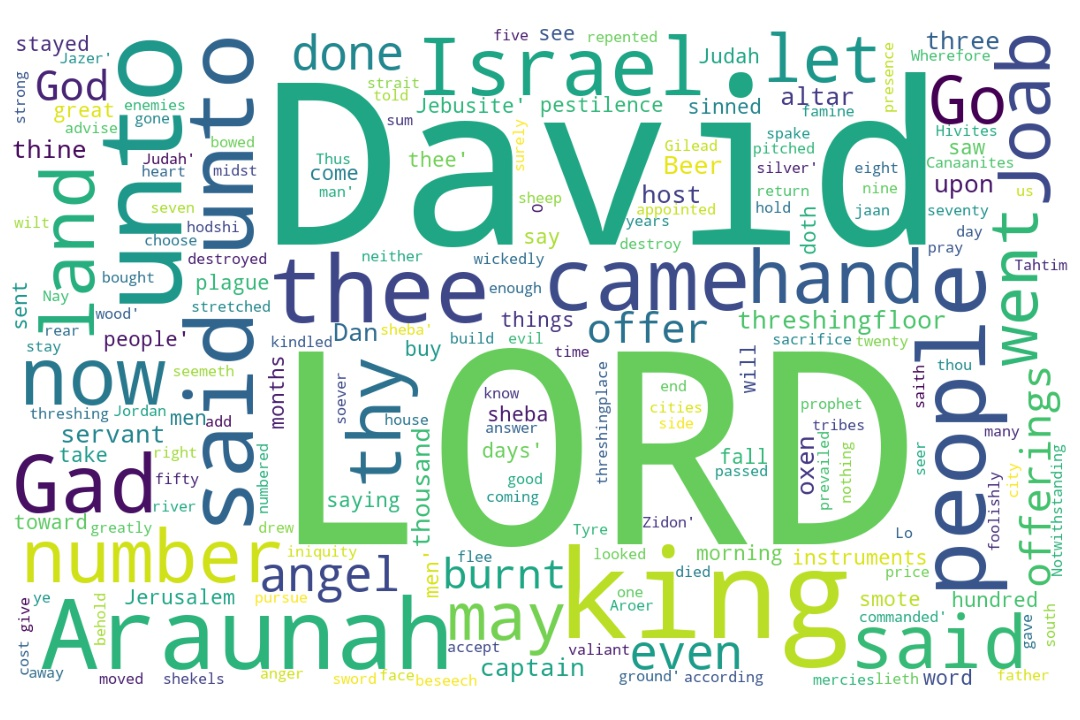
\includegraphics[width=\linewidth]{10OT-2Samuel/2Samuel24-WordCloud.jpg}
  \caption{1 Samuel 24 Word Cloud}
  \label{fig:1 Samuel 24 Word Cloud}
\end{figure}

%%%%%%%%%%%%%%%%%%%%%%%%%%%%%%%%%%%%%%%%%
%%%%%%%%%%%%%%%%%%%%%%%%%%%%%%%%%%%%%%%%%


\marginpar{\scriptsize \centering \fcolorbox{bone}{lime}{\textbf{CENSUS AND SACRIFICE}}\\ (2 Samuel 24:1--25) 
\begin{compactenum}[I.][8]
    \item A  \textbf{Census} \index[scripture]{2Samuel!2Sa 24:02}(2Sa 24:2)
    \item The  \textbf{Suggestion} \index[scripture]{2Samuel!2Sa 24:03}(2Sa 24:3) 
    \item The \textbf{Sum} \index[scripture]{2Samuel!2Sa 24:09} (2Sa 24:9)
    \item \textbf{Second} Thoughts \index[scripture]{2Samuel!2Sa 24:10} (2Sa 24:10)
    \item The \textbf{Sickness} \index[scripture]{2Samuel!2Sa 24:15} (2Sa 24:15)
    \item A \textbf{Sermon} \index[scripture]{2Samuel!2Sa 24:18} (2Sa 24:18) 
    \item The \textbf{Sacrifice} \index[scripture]{2Samuel!2Sa 24:25}(2Sa 24:25)
\end{compactenum} }

\footnote{\textcolor[cmyk]{0.99998,1,0,0}{\hyperlink{TOC}{Return to end of Table of Contents.}}}\footnote{\href{https://audiobible.com/bible/2_samuel_24.html}{\textcolor[cmyk]{0.99998,1,0,0}{2 Samuel 24 Audio}}}\textcolor[cmyk]{0.99998,1,0,0}{And again the anger of the LORD was kindled against Israel, and he moved  \fcolorbox{bone}{bone}{David} against them to say, \fcolorbox{bone}{lime}{Go, number Israel} and Judah.}
[2] \textcolor[cmyk]{0.99998,1,0,0}{For  \fcolorbox{bone}{bone}{the king}  \fcolorbox{bone}{bone}{said} to Joab the captain of the host, which \emph{was} with him, Go now through all the tribes of Israel, from Dan even to Beer-sheba, and number ye the people, that I may know the number of the people.}
[3] \textcolor[cmyk]{0.99998,1,0,0}{And Joab  \fcolorbox{bone}{bone}{said} unto  \fcolorbox{bone}{bone}{the king}, Now the LORD thy God add unto the people, how many soever they be, an hundredfold, and that the eyes of my lord  \fcolorbox{bone}{bone}{the king} may see \emph{it}: \fcolorbox{bone}{lime}{but why} doth my lord  \fcolorbox{bone}{bone}{the king} delight in this thing?}
[4] \textcolor[cmyk]{0.99998,1,0,0}{Notwithstanding the king's word prevailed against Joab, and against the captains of the host. And Joab and the captains of the host went out from the presence of  \fcolorbox{bone}{bone}{the king}, to number the people of Israel.}
[5] \textcolor[cmyk]{0.99998,1,0,0}{And they passed over Jordan, and pitched in Aroer, on the right side of the city that \emph{lieth} in the midst of the river of Gad, and toward Jazer:}\\
\\
\P \textcolor[cmyk]{0.99998,1,0,0}{Then they came to Gilead, and to the land of Tahtim-hodshi; and they came to Dan-jaan, and about to Zidon,}
[7] \textcolor[cmyk]{0.99998,1,0,0}{And came to the strong hold of Tyre, and to all the cities of the Hivites, and of the Canaanites: and they went out to the south of Judah, \emph{even} to Beer-sheba.}
[8] \textcolor[cmyk]{0.99998,1,0,0}{So when they had gone through all the land, they came to Jerusalem at the end of nine months and twenty days.}
[9] \textcolor[cmyk]{0.99998,1,0,0}{And Joab gave up \fcolorbox{bone}{lime}{the sum} of the number of the people unto  \fcolorbox{bone}{bone}{the king}: and there were in Israel eight hundred thousand valiant men that drew the sword; and the men of Judah \emph{were} five hundred thousand men.}\marginpar{\scriptsize \textcolor[rgb]{0.00,0.545,0.269}{$\rightarrow$800,000 + 500,000 = 1,300,000. }}\\
\\
\P \textcolor[cmyk]{0.99998,1,0,0}{And David's \fcolorbox{bone}{lime}{heart smote him} after that he had numbered the people. And  \fcolorbox{bone}{bone}{David}  \fcolorbox{bone}{bone}{said} unto the LORD, I have sinned greatly in that I have done: and now, I beseech thee, O LORD, take away the iniquity of thy servant; for I have done very foolishly.}
[11] \textcolor[cmyk]{0.99998,1,0,0}{For when David was up in the morning, the word of the LORD came unto the prophet Gad, David's seer, saying,}
[12] \textcolor[cmyk]{0.99998,1,0,0}{Go and say unto  \fcolorbox{bone}{bone}{David}, Thus saith the LORD, I offer thee three \emph{things}; choose thee one of them, that I may \emph{do} \emph{it} unto thee.}
[13] \textcolor[cmyk]{0.99998,1,0,0}{So Gad came to  \fcolorbox{bone}{bone}{David}, and told him, and  \fcolorbox{bone}{bone}{said} unto him, Shall seven years of famine come unto thee in thy land? or wilt thou flee three months before thine enemies, while they pursue thee? or that there be three days' pestilence in thy land? now advise, and see what answer I shall return to him that sent me.}
[14] \textcolor[cmyk]{0.99998,1,0,0}{And  \fcolorbox{bone}{bone}{David}  \fcolorbox{bone}{bone}{said} unto Gad, I am in a great strait: let us fall now into the hand of the LORD; for his mercies \emph{are} great: and let me not fall into the hand of man.}\\
\\
\P \textcolor[cmyk]{0.99998,1,0,0}{So the LORD sent a \fcolorbox{bone}{lime}{pestilence} upon Israel from the morning even to the time appointed: and there died of the people from Dan even to Beer-sheba seventy thousand men.}
[16] \textcolor[cmyk]{0.99998,1,0,0}{And when the angel stretched out his hand upon Jerusalem to destroy it, the LORD repented him of the evil, and  \fcolorbox{bone}{bone}{said} to the angel that destroyed the people, It is enough: stay now thine hand. And the angel of the LORD was by the threshingplace of Araunah the Jebusite.}
[17] \textcolor[cmyk]{0.99998,1,0,0}{And  \fcolorbox{bone}{bone}{David} spake unto the LORD when he saw the angel that smote the people, and  \fcolorbox{bone}{bone}{said}, Lo, I have sinned, and I have done wickedly: but these sheep, what have they done? let thine hand, I pray thee, be against me, and against my father's house.}\\
\\
\P \textcolor[cmyk]{0.99998,1,0,0}{And \fcolorbox{bone}{lime}{Gad came that day} to  \fcolorbox{bone}{bone}{David}, and  \fcolorbox{bone}{bone}{said} unto him, Go up, rear an altar unto the LORD in the threshingfloor of Araunah the Jebusite.}
[19] \textcolor[cmyk]{0.99998,1,0,0}{And  \fcolorbox{bone}{bone}{David}, according to the saying of Gad, went up as the LORD commanded.}
[20] \textcolor[cmyk]{0.99998,1,0,0}{And Araunah looked, and saw  \fcolorbox{bone}{bone}{the king} and his servants coming on toward him: and Araunah went out, and bowed himself before  \fcolorbox{bone}{bone}{the king} on his face upon the ground.}
[21] \textcolor[cmyk]{0.99998,1,0,0}{And Araunah  \fcolorbox{bone}{bone}{said}, Wherefore is my lord  \fcolorbox{bone}{bone}{the king} come to his servant? And  \fcolorbox{bone}{bone}{David}  \fcolorbox{bone}{bone}{said}, To buy the threshingfloor of thee, to build an altar unto the LORD, that the plague may be stayed from the people.}
[22] \textcolor[cmyk]{0.99998,1,0,0}{And Araunah  \fcolorbox{bone}{bone}{said} unto  \fcolorbox{bone}{bone}{David}, Let my lord  \fcolorbox{bone}{bone}{the king} take and offer up what \emph{seemeth} good unto him: behold, \emph{here} \emph{be} oxen for burnt sacrifice, and threshing instruments and \emph{other} instruments of the oxen for wood.}
[23] \textcolor[cmyk]{0.99998,1,0,0}{All these \emph{things} did Araunah, \emph{as} a king, give unto  \fcolorbox{bone}{bone}{the king}. And Araunah  \fcolorbox{bone}{bone}{said} unto  \fcolorbox{bone}{bone}{the king}, The LORD thy God accept thee.}
[24] \textcolor[cmyk]{0.99998,1,0,0}{And  \fcolorbox{bone}{bone}{the king}  \fcolorbox{bone}{bone}{said} unto Araunah, Nay; but I will surely buy \emph{it} of thee at a price: neither will I offer burnt offerings unto the LORD my God of that which doth cost me nothing. So  \fcolorbox{bone}{bone}{David} bought the threshingfloor and the oxen for fifty shekels of silver.}
[25] \textcolor[cmyk]{0.99998,1,0,0}{And  \fcolorbox{bone}{bone}{David} built there an altar unto the LORD, and offered burnt offerings and \fcolorbox{bone}{lime}{peace offerings}. So the LORD was intreated for the land, and the plague was stayed from Israel.}
\index[NWIV]{24!2Samuel!2Sa 24:1}\index[AWIP]{And!2Samuel!2Sa 24:1}\index[AWIP]{again!2Samuel!2Sa 24:1}\index[AWIP]{the!2Samuel!2Sa 24:1}\index[AWIP]{the!2Samuel!2Sa 24:1 (2)}\index[AWIP]{anger!2Samuel!2Sa 24:1}\index[AWIP]{of!2Samuel!2Sa 24:1}\index[AWIP]{LORD!2Samuel!2Sa 24:1}\index[AWIP]{was!2Samuel!2Sa 24:1}\index[AWIP]{kindled!2Samuel!2Sa 24:1}\index[AWIP]{against!2Samuel!2Sa 24:1}\index[AWIP]{against!2Samuel!2Sa 24:1 (2)}\index[AWIP]{Israel!2Samuel!2Sa 24:1}\index[AWIP]{Israel!2Samuel!2Sa 24:1 (2)}\index[AWIP]{and!2Samuel!2Sa 24:1}\index[AWIP]{and!2Samuel!2Sa 24:1 (2)}\index[AWIP]{he!2Samuel!2Sa 24:1}\index[AWIP]{moved!2Samuel!2Sa 24:1}\index[AWIP]{David!2Samuel!2Sa 24:1}\index[AWIP]{them!2Samuel!2Sa 24:1}\index[AWIP]{to!2Samuel!2Sa 24:1}\index[AWIP]{say!2Samuel!2Sa 24:1}\index[AWIP]{Go!2Samuel!2Sa 24:1}\index[AWIP]{number!2Samuel!2Sa 24:1}\index[AWIP]{Judah!2Samuel!2Sa 24:1}

\index[NWIV]{42!2Samuel!2Sa 24:2}\index[AWIP]{For!2Samuel!2Sa 24:2}\index[AWIP]{the!2Samuel!2Sa 24:2}\index[AWIP]{the!2Samuel!2Sa 24:2 (2)}\index[AWIP]{the!2Samuel!2Sa 24:2 (3)}\index[AWIP]{the!2Samuel!2Sa 24:2 (4)}\index[AWIP]{the!2Samuel!2Sa 24:2 (5)}\index[AWIP]{the!2Samuel!2Sa 24:2 (6)}\index[AWIP]{the!2Samuel!2Sa 24:2 (7)}\index[AWIP]{king!2Samuel!2Sa 24:2}\index[AWIP]{said!2Samuel!2Sa 24:2}\index[AWIP]{to!2Samuel!2Sa 24:2}\index[AWIP]{to!2Samuel!2Sa 24:2 (2)}\index[AWIP]{Joab!2Samuel!2Sa 24:2}\index[AWIP]{captain!2Samuel!2Sa 24:2}\index[AWIP]{of!2Samuel!2Sa 24:2}\index[AWIP]{of!2Samuel!2Sa 24:2 (2)}\index[AWIP]{of!2Samuel!2Sa 24:2 (3)}\index[AWIP]{host!2Samuel!2Sa 24:2}\index[AWIP]{which!2Samuel!2Sa 24:2}\index[AWIP]{\emph{was}!2Samuel!2Sa 24:2}\index[AWIP]{with!2Samuel!2Sa 24:2}\index[AWIP]{him!2Samuel!2Sa 24:2}\index[AWIP]{Go!2Samuel!2Sa 24:2}\index[AWIP]{now!2Samuel!2Sa 24:2}\index[AWIP]{through!2Samuel!2Sa 24:2}\index[AWIP]{all!2Samuel!2Sa 24:2}\index[AWIP]{tribes!2Samuel!2Sa 24:2}\index[AWIP]{Israel!2Samuel!2Sa 24:2}\index[AWIP]{from!2Samuel!2Sa 24:2}\index[AWIP]{Dan!2Samuel!2Sa 24:2}\index[AWIP]{even!2Samuel!2Sa 24:2}\index[AWIP]{Beer-sheba!2Samuel!2Sa 24:2}\index[AWIP]{and!2Samuel!2Sa 24:2}\index[AWIP]{number!2Samuel!2Sa 24:2}\index[AWIP]{number!2Samuel!2Sa 24:2 (2)}\index[AWIP]{ye!2Samuel!2Sa 24:2}\index[AWIP]{people!2Samuel!2Sa 24:2}\index[AWIP]{people!2Samuel!2Sa 24:2 (2)}\index[AWIP]{that!2Samuel!2Sa 24:2}\index[AWIP]{I!2Samuel!2Sa 24:2}\index[AWIP]{may!2Samuel!2Sa 24:2}\index[AWIP]{know!2Samuel!2Sa 24:2}\index[AWIP]{\emph{was}!2Samuel!2Sa 24:2}

\index[NWIV]{45!2Samuel!2Sa 24:3}\index[AWIP]{And!2Samuel!2Sa 24:3}\index[AWIP]{Joab!2Samuel!2Sa 24:3}\index[AWIP]{said!2Samuel!2Sa 24:3}\index[AWIP]{unto!2Samuel!2Sa 24:3}\index[AWIP]{unto!2Samuel!2Sa 24:3 (2)}\index[AWIP]{the!2Samuel!2Sa 24:3}\index[AWIP]{the!2Samuel!2Sa 24:3 (2)}\index[AWIP]{the!2Samuel!2Sa 24:3 (3)}\index[AWIP]{the!2Samuel!2Sa 24:3 (4)}\index[AWIP]{the!2Samuel!2Sa 24:3 (5)}\index[AWIP]{the!2Samuel!2Sa 24:3 (6)}\index[AWIP]{king!2Samuel!2Sa 24:3}\index[AWIP]{king!2Samuel!2Sa 24:3 (2)}\index[AWIP]{king!2Samuel!2Sa 24:3 (3)}\index[AWIP]{Now!2Samuel!2Sa 24:3}\index[AWIP]{LORD!2Samuel!2Sa 24:3}\index[AWIP]{thy!2Samuel!2Sa 24:3}\index[AWIP]{God!2Samuel!2Sa 24:3}\index[AWIP]{add!2Samuel!2Sa 24:3}\index[AWIP]{people!2Samuel!2Sa 24:3}\index[AWIP]{how!2Samuel!2Sa 24:3}\index[AWIP]{many!2Samuel!2Sa 24:3}\index[AWIP]{soever!2Samuel!2Sa 24:3}\index[AWIP]{they!2Samuel!2Sa 24:3}\index[AWIP]{be!2Samuel!2Sa 24:3}\index[AWIP]{an!2Samuel!2Sa 24:3}\index[AWIP]{hundredfold!2Samuel!2Sa 24:3}\index[AWIP]{and!2Samuel!2Sa 24:3}\index[AWIP]{that!2Samuel!2Sa 24:3}\index[AWIP]{eyes!2Samuel!2Sa 24:3}\index[AWIP]{of!2Samuel!2Sa 24:3}\index[AWIP]{my!2Samuel!2Sa 24:3}\index[AWIP]{my!2Samuel!2Sa 24:3 (2)}\index[AWIP]{lord!2Samuel!2Sa 24:3}\index[AWIP]{lord!2Samuel!2Sa 24:3 (2)}\index[AWIP]{may!2Samuel!2Sa 24:3}\index[AWIP]{see!2Samuel!2Sa 24:3}\index[AWIP]{\emph{it}!2Samuel!2Sa 24:3}\index[AWIP]{but!2Samuel!2Sa 24:3}\index[AWIP]{why!2Samuel!2Sa 24:3}\index[AWIP]{doth!2Samuel!2Sa 24:3}\index[AWIP]{delight!2Samuel!2Sa 24:3}\index[AWIP]{in!2Samuel!2Sa 24:3}\index[AWIP]{this!2Samuel!2Sa 24:3}\index[AWIP]{thing?!2Samuel!2Sa 24:3}\index[AWIP]{\emph{it}!2Samuel!2Sa 24:3}

\index[NWIV]{36!2Samuel!2Sa 24:4}\index[AWIP]{Notwithstanding!2Samuel!2Sa 24:4}\index[AWIP]{the!2Samuel!2Sa 24:4}\index[AWIP]{the!2Samuel!2Sa 24:4 (2)}\index[AWIP]{the!2Samuel!2Sa 24:4 (3)}\index[AWIP]{the!2Samuel!2Sa 24:4 (4)}\index[AWIP]{the!2Samuel!2Sa 24:4 (5)}\index[AWIP]{the!2Samuel!2Sa 24:4 (6)}\index[AWIP]{the!2Samuel!2Sa 24:4 (7)}\index[AWIP]{the!2Samuel!2Sa 24:4 (8)}\index[AWIP]{king's!2Samuel!2Sa 24:4}\index[AWIP]{word!2Samuel!2Sa 24:4}\index[AWIP]{prevailed!2Samuel!2Sa 24:4}\index[AWIP]{against!2Samuel!2Sa 24:4}\index[AWIP]{against!2Samuel!2Sa 24:4 (2)}\index[AWIP]{Joab!2Samuel!2Sa 24:4}\index[AWIP]{Joab!2Samuel!2Sa 24:4 (2)}\index[AWIP]{and!2Samuel!2Sa 24:4}\index[AWIP]{and!2Samuel!2Sa 24:4 (2)}\index[AWIP]{captains!2Samuel!2Sa 24:4}\index[AWIP]{captains!2Samuel!2Sa 24:4 (2)}\index[AWIP]{of!2Samuel!2Sa 24:4}\index[AWIP]{of!2Samuel!2Sa 24:4 (2)}\index[AWIP]{of!2Samuel!2Sa 24:4 (3)}\index[AWIP]{of!2Samuel!2Sa 24:4 (4)}\index[AWIP]{host!2Samuel!2Sa 24:4}\index[AWIP]{host!2Samuel!2Sa 24:4 (2)}\index[AWIP]{And!2Samuel!2Sa 24:4}\index[AWIP]{went!2Samuel!2Sa 24:4}\index[AWIP]{out!2Samuel!2Sa 24:4}\index[AWIP]{from!2Samuel!2Sa 24:4}\index[AWIP]{presence!2Samuel!2Sa 24:4}\index[AWIP]{king!2Samuel!2Sa 24:4}\index[AWIP]{to!2Samuel!2Sa 24:4}\index[AWIP]{number!2Samuel!2Sa 24:4}\index[AWIP]{people!2Samuel!2Sa 24:4}\index[AWIP]{Israel!2Samuel!2Sa 24:4}

\index[NWIV]{29!2Samuel!2Sa 24:5}\index[AWIP]{And!2Samuel!2Sa 24:5}\index[AWIP]{they!2Samuel!2Sa 24:5}\index[AWIP]{passed!2Samuel!2Sa 24:5}\index[AWIP]{over!2Samuel!2Sa 24:5}\index[AWIP]{Jordan!2Samuel!2Sa 24:5}\index[AWIP]{and!2Samuel!2Sa 24:5}\index[AWIP]{and!2Samuel!2Sa 24:5 (2)}\index[AWIP]{pitched!2Samuel!2Sa 24:5}\index[AWIP]{in!2Samuel!2Sa 24:5}\index[AWIP]{in!2Samuel!2Sa 24:5 (2)}\index[AWIP]{Aroer!2Samuel!2Sa 24:5}\index[AWIP]{on!2Samuel!2Sa 24:5}\index[AWIP]{the!2Samuel!2Sa 24:5}\index[AWIP]{the!2Samuel!2Sa 24:5 (2)}\index[AWIP]{the!2Samuel!2Sa 24:5 (3)}\index[AWIP]{the!2Samuel!2Sa 24:5 (4)}\index[AWIP]{right!2Samuel!2Sa 24:5}\index[AWIP]{side!2Samuel!2Sa 24:5}\index[AWIP]{of!2Samuel!2Sa 24:5}\index[AWIP]{of!2Samuel!2Sa 24:5 (2)}\index[AWIP]{of!2Samuel!2Sa 24:5 (3)}\index[AWIP]{city!2Samuel!2Sa 24:5}\index[AWIP]{that!2Samuel!2Sa 24:5}\index[AWIP]{\emph{lieth}!2Samuel!2Sa 24:5}\index[AWIP]{midst!2Samuel!2Sa 24:5}\index[AWIP]{river!2Samuel!2Sa 24:5}\index[AWIP]{Gad!2Samuel!2Sa 24:5}\index[AWIP]{toward!2Samuel!2Sa 24:5}\index[AWIP]{Jazer!2Samuel!2Sa 24:5}\index[AWIP]{\emph{lieth}!2Samuel!2Sa 24:5}

\index[NWIV]{20!2Samuel!2Sa 24:6}\index[AWIP]{Then!2Samuel!2Sa 24:6}\index[AWIP]{they!2Samuel!2Sa 24:6}\index[AWIP]{they!2Samuel!2Sa 24:6 (2)}\index[AWIP]{came!2Samuel!2Sa 24:6}\index[AWIP]{came!2Samuel!2Sa 24:6 (2)}\index[AWIP]{to!2Samuel!2Sa 24:6}\index[AWIP]{to!2Samuel!2Sa 24:6 (2)}\index[AWIP]{to!2Samuel!2Sa 24:6 (3)}\index[AWIP]{to!2Samuel!2Sa 24:6 (4)}\index[AWIP]{Gilead!2Samuel!2Sa 24:6}\index[AWIP]{and!2Samuel!2Sa 24:6}\index[AWIP]{and!2Samuel!2Sa 24:6 (2)}\index[AWIP]{and!2Samuel!2Sa 24:6 (3)}\index[AWIP]{the!2Samuel!2Sa 24:6}\index[AWIP]{land!2Samuel!2Sa 24:6}\index[AWIP]{of!2Samuel!2Sa 24:6}\index[AWIP]{Tahtim-hodshi!2Samuel!2Sa 24:6}\index[AWIP]{Dan-jaan!2Samuel!2Sa 24:6}\index[AWIP]{about!2Samuel!2Sa 24:6}\index[AWIP]{Zidon!2Samuel!2Sa 24:6}

\index[NWIV]{32!2Samuel!2Sa 24:7}\index[AWIP]{And!2Samuel!2Sa 24:7}\index[AWIP]{came!2Samuel!2Sa 24:7}\index[AWIP]{to!2Samuel!2Sa 24:7}\index[AWIP]{to!2Samuel!2Sa 24:7 (2)}\index[AWIP]{to!2Samuel!2Sa 24:7 (3)}\index[AWIP]{to!2Samuel!2Sa 24:7 (4)}\index[AWIP]{the!2Samuel!2Sa 24:7}\index[AWIP]{the!2Samuel!2Sa 24:7 (2)}\index[AWIP]{the!2Samuel!2Sa 24:7 (3)}\index[AWIP]{the!2Samuel!2Sa 24:7 (4)}\index[AWIP]{the!2Samuel!2Sa 24:7 (5)}\index[AWIP]{strong!2Samuel!2Sa 24:7}\index[AWIP]{hold!2Samuel!2Sa 24:7}\index[AWIP]{of!2Samuel!2Sa 24:7}\index[AWIP]{of!2Samuel!2Sa 24:7 (2)}\index[AWIP]{of!2Samuel!2Sa 24:7 (3)}\index[AWIP]{of!2Samuel!2Sa 24:7 (4)}\index[AWIP]{Tyre!2Samuel!2Sa 24:7}\index[AWIP]{and!2Samuel!2Sa 24:7}\index[AWIP]{and!2Samuel!2Sa 24:7 (2)}\index[AWIP]{and!2Samuel!2Sa 24:7 (3)}\index[AWIP]{all!2Samuel!2Sa 24:7}\index[AWIP]{cities!2Samuel!2Sa 24:7}\index[AWIP]{Hivites!2Samuel!2Sa 24:7}\index[AWIP]{Canaanites!2Samuel!2Sa 24:7}\index[AWIP]{they!2Samuel!2Sa 24:7}\index[AWIP]{went!2Samuel!2Sa 24:7}\index[AWIP]{out!2Samuel!2Sa 24:7}\index[AWIP]{south!2Samuel!2Sa 24:7}\index[AWIP]{Judah!2Samuel!2Sa 24:7}\index[AWIP]{\emph{even}!2Samuel!2Sa 24:7}\index[AWIP]{Beer-sheba!2Samuel!2Sa 24:7}\index[AWIP]{\emph{even}!2Samuel!2Sa 24:7}

\index[NWIV]{22!2Samuel!2Sa 24:8}\index[AWIP]{So!2Samuel!2Sa 24:8}\index[AWIP]{when!2Samuel!2Sa 24:8}\index[AWIP]{they!2Samuel!2Sa 24:8}\index[AWIP]{they!2Samuel!2Sa 24:8 (2)}\index[AWIP]{had!2Samuel!2Sa 24:8}\index[AWIP]{gone!2Samuel!2Sa 24:8}\index[AWIP]{through!2Samuel!2Sa 24:8}\index[AWIP]{all!2Samuel!2Sa 24:8}\index[AWIP]{the!2Samuel!2Sa 24:8}\index[AWIP]{the!2Samuel!2Sa 24:8 (2)}\index[AWIP]{land!2Samuel!2Sa 24:8}\index[AWIP]{came!2Samuel!2Sa 24:8}\index[AWIP]{to!2Samuel!2Sa 24:8}\index[AWIP]{Jerusalem!2Samuel!2Sa 24:8}\index[AWIP]{at!2Samuel!2Sa 24:8}\index[AWIP]{end!2Samuel!2Sa 24:8}\index[AWIP]{of!2Samuel!2Sa 24:8}\index[AWIP]{nine!2Samuel!2Sa 24:8}\index[AWIP]{months!2Samuel!2Sa 24:8}\index[AWIP]{and!2Samuel!2Sa 24:8}\index[AWIP]{twenty!2Samuel!2Sa 24:8}\index[AWIP]{days!2Samuel!2Sa 24:8}

\index[NWIV]{39!2Samuel!2Sa 24:9}\index[AWIP]{And!2Samuel!2Sa 24:9}\index[AWIP]{Joab!2Samuel!2Sa 24:9}\index[AWIP]{gave!2Samuel!2Sa 24:9}\index[AWIP]{up!2Samuel!2Sa 24:9}\index[AWIP]{the!2Samuel!2Sa 24:9}\index[AWIP]{the!2Samuel!2Sa 24:9 (2)}\index[AWIP]{the!2Samuel!2Sa 24:9 (3)}\index[AWIP]{the!2Samuel!2Sa 24:9 (4)}\index[AWIP]{the!2Samuel!2Sa 24:9 (5)}\index[AWIP]{the!2Samuel!2Sa 24:9 (6)}\index[AWIP]{sum!2Samuel!2Sa 24:9}\index[AWIP]{of!2Samuel!2Sa 24:9}\index[AWIP]{of!2Samuel!2Sa 24:9 (2)}\index[AWIP]{of!2Samuel!2Sa 24:9 (3)}\index[AWIP]{number!2Samuel!2Sa 24:9}\index[AWIP]{people!2Samuel!2Sa 24:9}\index[AWIP]{unto!2Samuel!2Sa 24:9}\index[AWIP]{king!2Samuel!2Sa 24:9}\index[AWIP]{and!2Samuel!2Sa 24:9}\index[AWIP]{and!2Samuel!2Sa 24:9 (2)}\index[AWIP]{there!2Samuel!2Sa 24:9}\index[AWIP]{were!2Samuel!2Sa 24:9}\index[AWIP]{in!2Samuel!2Sa 24:9}\index[AWIP]{Israel!2Samuel!2Sa 24:9}\index[AWIP]{eight!2Samuel!2Sa 24:9}\index[AWIP]{hundred!2Samuel!2Sa 24:9}\index[AWIP]{hundred!2Samuel!2Sa 24:9 (2)}\index[AWIP]{thousand!2Samuel!2Sa 24:9}\index[AWIP]{thousand!2Samuel!2Sa 24:9 (2)}\index[AWIP]{valiant!2Samuel!2Sa 24:9}\index[AWIP]{men!2Samuel!2Sa 24:9}\index[AWIP]{men!2Samuel!2Sa 24:9 (2)}\index[AWIP]{men!2Samuel!2Sa 24:9 (3)}\index[AWIP]{that!2Samuel!2Sa 24:9}\index[AWIP]{drew!2Samuel!2Sa 24:9}\index[AWIP]{sword!2Samuel!2Sa 24:9}\index[AWIP]{Judah!2Samuel!2Sa 24:9}\index[AWIP]{\emph{were}!2Samuel!2Sa 24:9}\index[AWIP]{five!2Samuel!2Sa 24:9}\index[AWIP]{\emph{were}!2Samuel!2Sa 24:9}

\index[NWIV]{47!2Samuel!2Sa 24:10}\index[AWIP]{And!2Samuel!2Sa 24:10}\index[AWIP]{And!2Samuel!2Sa 24:10 (2)}\index[AWIP]{David's!2Samuel!2Sa 24:10}\index[AWIP]{heart!2Samuel!2Sa 24:10}\index[AWIP]{smote!2Samuel!2Sa 24:10}\index[AWIP]{him!2Samuel!2Sa 24:10}\index[AWIP]{after!2Samuel!2Sa 24:10}\index[AWIP]{that!2Samuel!2Sa 24:10}\index[AWIP]{that!2Samuel!2Sa 24:10 (2)}\index[AWIP]{he!2Samuel!2Sa 24:10}\index[AWIP]{had!2Samuel!2Sa 24:10}\index[AWIP]{numbered!2Samuel!2Sa 24:10}\index[AWIP]{the!2Samuel!2Sa 24:10}\index[AWIP]{the!2Samuel!2Sa 24:10 (2)}\index[AWIP]{the!2Samuel!2Sa 24:10 (3)}\index[AWIP]{people!2Samuel!2Sa 24:10}\index[AWIP]{David!2Samuel!2Sa 24:10}\index[AWIP]{said!2Samuel!2Sa 24:10}\index[AWIP]{unto!2Samuel!2Sa 24:10}\index[AWIP]{LORD!2Samuel!2Sa 24:10}\index[AWIP]{LORD!2Samuel!2Sa 24:10 (2)}\index[AWIP]{I!2Samuel!2Sa 24:10}\index[AWIP]{I!2Samuel!2Sa 24:10 (2)}\index[AWIP]{I!2Samuel!2Sa 24:10 (3)}\index[AWIP]{I!2Samuel!2Sa 24:10 (4)}\index[AWIP]{have!2Samuel!2Sa 24:10}\index[AWIP]{have!2Samuel!2Sa 24:10 (2)}\index[AWIP]{have!2Samuel!2Sa 24:10 (3)}\index[AWIP]{sinned!2Samuel!2Sa 24:10}\index[AWIP]{greatly!2Samuel!2Sa 24:10}\index[AWIP]{in!2Samuel!2Sa 24:10}\index[AWIP]{done!2Samuel!2Sa 24:10}\index[AWIP]{done!2Samuel!2Sa 24:10 (2)}\index[AWIP]{and!2Samuel!2Sa 24:10}\index[AWIP]{now!2Samuel!2Sa 24:10}\index[AWIP]{beseech!2Samuel!2Sa 24:10}\index[AWIP]{thee!2Samuel!2Sa 24:10}\index[AWIP]{O!2Samuel!2Sa 24:10}\index[AWIP]{take!2Samuel!2Sa 24:10}\index[AWIP]{away!2Samuel!2Sa 24:10}\index[AWIP]{iniquity!2Samuel!2Sa 24:10}\index[AWIP]{of!2Samuel!2Sa 24:10}\index[AWIP]{thy!2Samuel!2Sa 24:10}\index[AWIP]{servant!2Samuel!2Sa 24:10}\index[AWIP]{for!2Samuel!2Sa 24:10}\index[AWIP]{very!2Samuel!2Sa 24:10}\index[AWIP]{foolishly!2Samuel!2Sa 24:10}

\index[NWIV]{21!2Samuel!2Sa 24:11}\index[AWIP]{For!2Samuel!2Sa 24:11}\index[AWIP]{when!2Samuel!2Sa 24:11}\index[AWIP]{David!2Samuel!2Sa 24:11}\index[AWIP]{was!2Samuel!2Sa 24:11}\index[AWIP]{up!2Samuel!2Sa 24:11}\index[AWIP]{in!2Samuel!2Sa 24:11}\index[AWIP]{the!2Samuel!2Sa 24:11}\index[AWIP]{the!2Samuel!2Sa 24:11 (2)}\index[AWIP]{the!2Samuel!2Sa 24:11 (3)}\index[AWIP]{the!2Samuel!2Sa 24:11 (4)}\index[AWIP]{morning!2Samuel!2Sa 24:11}\index[AWIP]{word!2Samuel!2Sa 24:11}\index[AWIP]{of!2Samuel!2Sa 24:11}\index[AWIP]{LORD!2Samuel!2Sa 24:11}\index[AWIP]{came!2Samuel!2Sa 24:11}\index[AWIP]{unto!2Samuel!2Sa 24:11}\index[AWIP]{prophet!2Samuel!2Sa 24:11}\index[AWIP]{Gad!2Samuel!2Sa 24:11}\index[AWIP]{David's!2Samuel!2Sa 24:11}\index[AWIP]{seer!2Samuel!2Sa 24:11}\index[AWIP]{saying!2Samuel!2Sa 24:11}

\index[NWIV]{26!2Samuel!2Sa 24:12}\index[AWIP]{Go!2Samuel!2Sa 24:12}\index[AWIP]{and!2Samuel!2Sa 24:12}\index[AWIP]{say!2Samuel!2Sa 24:12}\index[AWIP]{unto!2Samuel!2Sa 24:12}\index[AWIP]{unto!2Samuel!2Sa 24:12 (2)}\index[AWIP]{David!2Samuel!2Sa 24:12}\index[AWIP]{Thus!2Samuel!2Sa 24:12}\index[AWIP]{saith!2Samuel!2Sa 24:12}\index[AWIP]{the!2Samuel!2Sa 24:12}\index[AWIP]{LORD!2Samuel!2Sa 24:12}\index[AWIP]{I!2Samuel!2Sa 24:12}\index[AWIP]{I!2Samuel!2Sa 24:12 (2)}\index[AWIP]{offer!2Samuel!2Sa 24:12}\index[AWIP]{thee!2Samuel!2Sa 24:12}\index[AWIP]{thee!2Samuel!2Sa 24:12 (2)}\index[AWIP]{thee!2Samuel!2Sa 24:12 (3)}\index[AWIP]{three!2Samuel!2Sa 24:12}\index[AWIP]{\emph{things}!2Samuel!2Sa 24:12}\index[AWIP]{choose!2Samuel!2Sa 24:12}\index[AWIP]{one!2Samuel!2Sa 24:12}\index[AWIP]{of!2Samuel!2Sa 24:12}\index[AWIP]{them!2Samuel!2Sa 24:12}\index[AWIP]{that!2Samuel!2Sa 24:12}\index[AWIP]{may!2Samuel!2Sa 24:12}\index[AWIP]{\emph{do}!2Samuel!2Sa 24:12}\index[AWIP]{\emph{it}!2Samuel!2Sa 24:12}\index[AWIP]{\emph{things}!2Samuel!2Sa 24:12}\index[AWIP]{\emph{do}!2Samuel!2Sa 24:12}\index[AWIP]{\emph{it}!2Samuel!2Sa 24:12}

\index[NWIV]{60!2Samuel!2Sa 24:13}\index[AWIP]{So!2Samuel!2Sa 24:13}\index[AWIP]{Gad!2Samuel!2Sa 24:13}\index[AWIP]{came!2Samuel!2Sa 24:13}\index[AWIP]{to!2Samuel!2Sa 24:13}\index[AWIP]{to!2Samuel!2Sa 24:13 (2)}\index[AWIP]{David!2Samuel!2Sa 24:13}\index[AWIP]{and!2Samuel!2Sa 24:13}\index[AWIP]{and!2Samuel!2Sa 24:13 (2)}\index[AWIP]{and!2Samuel!2Sa 24:13 (3)}\index[AWIP]{told!2Samuel!2Sa 24:13}\index[AWIP]{him!2Samuel!2Sa 24:13}\index[AWIP]{him!2Samuel!2Sa 24:13 (2)}\index[AWIP]{him!2Samuel!2Sa 24:13 (3)}\index[AWIP]{said!2Samuel!2Sa 24:13}\index[AWIP]{unto!2Samuel!2Sa 24:13}\index[AWIP]{unto!2Samuel!2Sa 24:13 (2)}\index[AWIP]{Shall!2Samuel!2Sa 24:13}\index[AWIP]{seven!2Samuel!2Sa 24:13}\index[AWIP]{years!2Samuel!2Sa 24:13}\index[AWIP]{of!2Samuel!2Sa 24:13}\index[AWIP]{famine!2Samuel!2Sa 24:13}\index[AWIP]{come!2Samuel!2Sa 24:13}\index[AWIP]{thee!2Samuel!2Sa 24:13}\index[AWIP]{in!2Samuel!2Sa 24:13}\index[AWIP]{in!2Samuel!2Sa 24:13 (2)}\index[AWIP]{thy!2Samuel!2Sa 24:13}\index[AWIP]{thy!2Samuel!2Sa 24:13 (2)}\index[AWIP]{land?!2Samuel!2Sa 24:13}\index[AWIP]{land?!2Samuel!2Sa 24:13 (2)}\index[AWIP]{or!2Samuel!2Sa 24:13}\index[AWIP]{or!2Samuel!2Sa 24:13 (2)}\index[AWIP]{wilt!2Samuel!2Sa 24:13}\index[AWIP]{thou!2Samuel!2Sa 24:13}\index[AWIP]{flee!2Samuel!2Sa 24:13}\index[AWIP]{three!2Samuel!2Sa 24:13}\index[AWIP]{three!2Samuel!2Sa 24:13 (2)}\index[AWIP]{months!2Samuel!2Sa 24:13}\index[AWIP]{before!2Samuel!2Sa 24:13}\index[AWIP]{thine!2Samuel!2Sa 24:13}\index[AWIP]{enemies!2Samuel!2Sa 24:13}\index[AWIP]{while!2Samuel!2Sa 24:13}\index[AWIP]{they!2Samuel!2Sa 24:13}\index[AWIP]{pursue!2Samuel!2Sa 24:13}\index[AWIP]{thee?!2Samuel!2Sa 24:13}\index[AWIP]{that!2Samuel!2Sa 24:13}\index[AWIP]{that!2Samuel!2Sa 24:13 (2)}\index[AWIP]{there!2Samuel!2Sa 24:13}\index[AWIP]{be!2Samuel!2Sa 24:13}\index[AWIP]{days'!2Samuel!2Sa 24:13}\index[AWIP]{pestilence!2Samuel!2Sa 24:13}\index[AWIP]{now!2Samuel!2Sa 24:13}\index[AWIP]{advise!2Samuel!2Sa 24:13}\index[AWIP]{see!2Samuel!2Sa 24:13}\index[AWIP]{what!2Samuel!2Sa 24:13}\index[AWIP]{answer!2Samuel!2Sa 24:13}\index[AWIP]{I!2Samuel!2Sa 24:13}\index[AWIP]{shall!2Samuel!2Sa 24:13}\index[AWIP]{return!2Samuel!2Sa 24:13}\index[AWIP]{sent!2Samuel!2Sa 24:13}\index[AWIP]{me!2Samuel!2Sa 24:13}

\index[NWIV]{36!2Samuel!2Sa 24:14}\index[AWIP]{And!2Samuel!2Sa 24:14}\index[AWIP]{David!2Samuel!2Sa 24:14}\index[AWIP]{said!2Samuel!2Sa 24:14}\index[AWIP]{unto!2Samuel!2Sa 24:14}\index[AWIP]{Gad!2Samuel!2Sa 24:14}\index[AWIP]{I!2Samuel!2Sa 24:14}\index[AWIP]{am!2Samuel!2Sa 24:14}\index[AWIP]{in!2Samuel!2Sa 24:14}\index[AWIP]{a!2Samuel!2Sa 24:14}\index[AWIP]{great!2Samuel!2Sa 24:14}\index[AWIP]{great!2Samuel!2Sa 24:14 (2)}\index[AWIP]{strait!2Samuel!2Sa 24:14}\index[AWIP]{let!2Samuel!2Sa 24:14}\index[AWIP]{let!2Samuel!2Sa 24:14 (2)}\index[AWIP]{us!2Samuel!2Sa 24:14}\index[AWIP]{fall!2Samuel!2Sa 24:14}\index[AWIP]{fall!2Samuel!2Sa 24:14 (2)}\index[AWIP]{now!2Samuel!2Sa 24:14}\index[AWIP]{into!2Samuel!2Sa 24:14}\index[AWIP]{into!2Samuel!2Sa 24:14 (2)}\index[AWIP]{the!2Samuel!2Sa 24:14}\index[AWIP]{the!2Samuel!2Sa 24:14 (2)}\index[AWIP]{the!2Samuel!2Sa 24:14 (3)}\index[AWIP]{hand!2Samuel!2Sa 24:14}\index[AWIP]{hand!2Samuel!2Sa 24:14 (2)}\index[AWIP]{of!2Samuel!2Sa 24:14}\index[AWIP]{of!2Samuel!2Sa 24:14 (2)}\index[AWIP]{LORD!2Samuel!2Sa 24:14}\index[AWIP]{for!2Samuel!2Sa 24:14}\index[AWIP]{his!2Samuel!2Sa 24:14}\index[AWIP]{mercies!2Samuel!2Sa 24:14}\index[AWIP]{\emph{are}!2Samuel!2Sa 24:14}\index[AWIP]{and!2Samuel!2Sa 24:14}\index[AWIP]{me!2Samuel!2Sa 24:14}\index[AWIP]{not!2Samuel!2Sa 24:14}\index[AWIP]{man!2Samuel!2Sa 24:14}\index[AWIP]{\emph{are}!2Samuel!2Sa 24:14}

\index[NWIV]{30!2Samuel!2Sa 24:15}\index[AWIP]{So!2Samuel!2Sa 24:15}\index[AWIP]{the!2Samuel!2Sa 24:15}\index[AWIP]{the!2Samuel!2Sa 24:15 (2)}\index[AWIP]{the!2Samuel!2Sa 24:15 (3)}\index[AWIP]{the!2Samuel!2Sa 24:15 (4)}\index[AWIP]{LORD!2Samuel!2Sa 24:15}\index[AWIP]{sent!2Samuel!2Sa 24:15}\index[AWIP]{a!2Samuel!2Sa 24:15}\index[AWIP]{pestilence!2Samuel!2Sa 24:15}\index[AWIP]{upon!2Samuel!2Sa 24:15}\index[AWIP]{Israel!2Samuel!2Sa 24:15}\index[AWIP]{from!2Samuel!2Sa 24:15}\index[AWIP]{from!2Samuel!2Sa 24:15 (2)}\index[AWIP]{morning!2Samuel!2Sa 24:15}\index[AWIP]{even!2Samuel!2Sa 24:15}\index[AWIP]{even!2Samuel!2Sa 24:15 (2)}\index[AWIP]{to!2Samuel!2Sa 24:15}\index[AWIP]{to!2Samuel!2Sa 24:15 (2)}\index[AWIP]{time!2Samuel!2Sa 24:15}\index[AWIP]{appointed!2Samuel!2Sa 24:15}\index[AWIP]{and!2Samuel!2Sa 24:15}\index[AWIP]{there!2Samuel!2Sa 24:15}\index[AWIP]{died!2Samuel!2Sa 24:15}\index[AWIP]{of!2Samuel!2Sa 24:15}\index[AWIP]{people!2Samuel!2Sa 24:15}\index[AWIP]{Dan!2Samuel!2Sa 24:15}\index[AWIP]{Beer-sheba!2Samuel!2Sa 24:15}\index[AWIP]{seventy!2Samuel!2Sa 24:15}\index[AWIP]{thousand!2Samuel!2Sa 24:15}\index[AWIP]{men!2Samuel!2Sa 24:15}

\index[NWIV]{50!2Samuel!2Sa 24:16}\index[AWIP]{And!2Samuel!2Sa 24:16}\index[AWIP]{And!2Samuel!2Sa 24:16 (2)}\index[AWIP]{when!2Samuel!2Sa 24:16}\index[AWIP]{the!2Samuel!2Sa 24:16}\index[AWIP]{the!2Samuel!2Sa 24:16 (2)}\index[AWIP]{the!2Samuel!2Sa 24:16 (3)}\index[AWIP]{the!2Samuel!2Sa 24:16 (4)}\index[AWIP]{the!2Samuel!2Sa 24:16 (5)}\index[AWIP]{the!2Samuel!2Sa 24:16 (6)}\index[AWIP]{the!2Samuel!2Sa 24:16 (7)}\index[AWIP]{the!2Samuel!2Sa 24:16 (8)}\index[AWIP]{the!2Samuel!2Sa 24:16 (9)}\index[AWIP]{angel!2Samuel!2Sa 24:16}\index[AWIP]{angel!2Samuel!2Sa 24:16 (2)}\index[AWIP]{angel!2Samuel!2Sa 24:16 (3)}\index[AWIP]{stretched!2Samuel!2Sa 24:16}\index[AWIP]{out!2Samuel!2Sa 24:16}\index[AWIP]{his!2Samuel!2Sa 24:16}\index[AWIP]{hand!2Samuel!2Sa 24:16}\index[AWIP]{hand!2Samuel!2Sa 24:16 (2)}\index[AWIP]{upon!2Samuel!2Sa 24:16}\index[AWIP]{Jerusalem!2Samuel!2Sa 24:16}\index[AWIP]{to!2Samuel!2Sa 24:16}\index[AWIP]{to!2Samuel!2Sa 24:16 (2)}\index[AWIP]{destroy!2Samuel!2Sa 24:16}\index[AWIP]{it!2Samuel!2Sa 24:16}\index[AWIP]{LORD!2Samuel!2Sa 24:16}\index[AWIP]{LORD!2Samuel!2Sa 24:16 (2)}\index[AWIP]{repented!2Samuel!2Sa 24:16}\index[AWIP]{him!2Samuel!2Sa 24:16}\index[AWIP]{of!2Samuel!2Sa 24:16}\index[AWIP]{of!2Samuel!2Sa 24:16 (2)}\index[AWIP]{of!2Samuel!2Sa 24:16 (3)}\index[AWIP]{evil!2Samuel!2Sa 24:16}\index[AWIP]{and!2Samuel!2Sa 24:16}\index[AWIP]{said!2Samuel!2Sa 24:16}\index[AWIP]{that!2Samuel!2Sa 24:16}\index[AWIP]{destroyed!2Samuel!2Sa 24:16}\index[AWIP]{people!2Samuel!2Sa 24:16}\index[AWIP]{It!2Samuel!2Sa 24:16}\index[AWIP]{is!2Samuel!2Sa 24:16}\index[AWIP]{enough!2Samuel!2Sa 24:16}\index[AWIP]{stay!2Samuel!2Sa 24:16}\index[AWIP]{now!2Samuel!2Sa 24:16}\index[AWIP]{thine!2Samuel!2Sa 24:16}\index[AWIP]{was!2Samuel!2Sa 24:16}\index[AWIP]{by!2Samuel!2Sa 24:16}\index[AWIP]{threshingplace!2Samuel!2Sa 24:16}\index[AWIP]{Araunah!2Samuel!2Sa 24:16}\index[AWIP]{Jebusite!2Samuel!2Sa 24:16}

\index[NWIV]{47!2Samuel!2Sa 24:17}\index[AWIP]{And!2Samuel!2Sa 24:17}\index[AWIP]{David!2Samuel!2Sa 24:17}\index[AWIP]{spake!2Samuel!2Sa 24:17}\index[AWIP]{unto!2Samuel!2Sa 24:17}\index[AWIP]{the!2Samuel!2Sa 24:17}\index[AWIP]{the!2Samuel!2Sa 24:17 (2)}\index[AWIP]{the!2Samuel!2Sa 24:17 (3)}\index[AWIP]{LORD!2Samuel!2Sa 24:17}\index[AWIP]{when!2Samuel!2Sa 24:17}\index[AWIP]{he!2Samuel!2Sa 24:17}\index[AWIP]{saw!2Samuel!2Sa 24:17}\index[AWIP]{angel!2Samuel!2Sa 24:17}\index[AWIP]{that!2Samuel!2Sa 24:17}\index[AWIP]{smote!2Samuel!2Sa 24:17}\index[AWIP]{people!2Samuel!2Sa 24:17}\index[AWIP]{and!2Samuel!2Sa 24:17}\index[AWIP]{and!2Samuel!2Sa 24:17 (2)}\index[AWIP]{and!2Samuel!2Sa 24:17 (3)}\index[AWIP]{said!2Samuel!2Sa 24:17}\index[AWIP]{Lo!2Samuel!2Sa 24:17}\index[AWIP]{I!2Samuel!2Sa 24:17}\index[AWIP]{I!2Samuel!2Sa 24:17 (2)}\index[AWIP]{I!2Samuel!2Sa 24:17 (3)}\index[AWIP]{have!2Samuel!2Sa 24:17}\index[AWIP]{have!2Samuel!2Sa 24:17 (2)}\index[AWIP]{have!2Samuel!2Sa 24:17 (3)}\index[AWIP]{sinned!2Samuel!2Sa 24:17}\index[AWIP]{done!2Samuel!2Sa 24:17}\index[AWIP]{wickedly!2Samuel!2Sa 24:17}\index[AWIP]{but!2Samuel!2Sa 24:17}\index[AWIP]{these!2Samuel!2Sa 24:17}\index[AWIP]{sheep!2Samuel!2Sa 24:17}\index[AWIP]{what!2Samuel!2Sa 24:17}\index[AWIP]{they!2Samuel!2Sa 24:17}\index[AWIP]{done?!2Samuel!2Sa 24:17}\index[AWIP]{let!2Samuel!2Sa 24:17}\index[AWIP]{thine!2Samuel!2Sa 24:17}\index[AWIP]{hand!2Samuel!2Sa 24:17}\index[AWIP]{pray!2Samuel!2Sa 24:17}\index[AWIP]{thee!2Samuel!2Sa 24:17}\index[AWIP]{be!2Samuel!2Sa 24:17}\index[AWIP]{against!2Samuel!2Sa 24:17}\index[AWIP]{against!2Samuel!2Sa 24:17 (2)}\index[AWIP]{me!2Samuel!2Sa 24:17}\index[AWIP]{my!2Samuel!2Sa 24:17}\index[AWIP]{father's!2Samuel!2Sa 24:17}\index[AWIP]{house!2Samuel!2Sa 24:17}

\index[NWIV]{26!2Samuel!2Sa 24:18}\index[AWIP]{And!2Samuel!2Sa 24:18}\index[AWIP]{Gad!2Samuel!2Sa 24:18}\index[AWIP]{came!2Samuel!2Sa 24:18}\index[AWIP]{that!2Samuel!2Sa 24:18}\index[AWIP]{day!2Samuel!2Sa 24:18}\index[AWIP]{to!2Samuel!2Sa 24:18}\index[AWIP]{David!2Samuel!2Sa 24:18}\index[AWIP]{and!2Samuel!2Sa 24:18}\index[AWIP]{said!2Samuel!2Sa 24:18}\index[AWIP]{unto!2Samuel!2Sa 24:18}\index[AWIP]{unto!2Samuel!2Sa 24:18 (2)}\index[AWIP]{him!2Samuel!2Sa 24:18}\index[AWIP]{Go!2Samuel!2Sa 24:18}\index[AWIP]{up!2Samuel!2Sa 24:18}\index[AWIP]{rear!2Samuel!2Sa 24:18}\index[AWIP]{an!2Samuel!2Sa 24:18}\index[AWIP]{altar!2Samuel!2Sa 24:18}\index[AWIP]{the!2Samuel!2Sa 24:18}\index[AWIP]{the!2Samuel!2Sa 24:18 (2)}\index[AWIP]{the!2Samuel!2Sa 24:18 (3)}\index[AWIP]{LORD!2Samuel!2Sa 24:18}\index[AWIP]{in!2Samuel!2Sa 24:18}\index[AWIP]{threshingfloor!2Samuel!2Sa 24:18}\index[AWIP]{of!2Samuel!2Sa 24:18}\index[AWIP]{Araunah!2Samuel!2Sa 24:18}\index[AWIP]{Jebusite!2Samuel!2Sa 24:18}

\index[NWIV]{14!2Samuel!2Sa 24:19}\index[AWIP]{And!2Samuel!2Sa 24:19}\index[AWIP]{David!2Samuel!2Sa 24:19}\index[AWIP]{according!2Samuel!2Sa 24:19}\index[AWIP]{to!2Samuel!2Sa 24:19}\index[AWIP]{the!2Samuel!2Sa 24:19}\index[AWIP]{the!2Samuel!2Sa 24:19 (2)}\index[AWIP]{saying!2Samuel!2Sa 24:19}\index[AWIP]{of!2Samuel!2Sa 24:19}\index[AWIP]{Gad!2Samuel!2Sa 24:19}\index[AWIP]{went!2Samuel!2Sa 24:19}\index[AWIP]{up!2Samuel!2Sa 24:19}\index[AWIP]{as!2Samuel!2Sa 24:19}\index[AWIP]{LORD!2Samuel!2Sa 24:19}\index[AWIP]{commanded!2Samuel!2Sa 24:19}

\index[NWIV]{30!2Samuel!2Sa 24:20}\index[AWIP]{And!2Samuel!2Sa 24:20}\index[AWIP]{Araunah!2Samuel!2Sa 24:20}\index[AWIP]{Araunah!2Samuel!2Sa 24:20 (2)}\index[AWIP]{looked!2Samuel!2Sa 24:20}\index[AWIP]{and!2Samuel!2Sa 24:20}\index[AWIP]{and!2Samuel!2Sa 24:20 (2)}\index[AWIP]{and!2Samuel!2Sa 24:20 (3)}\index[AWIP]{and!2Samuel!2Sa 24:20 (4)}\index[AWIP]{saw!2Samuel!2Sa 24:20}\index[AWIP]{the!2Samuel!2Sa 24:20}\index[AWIP]{the!2Samuel!2Sa 24:20 (2)}\index[AWIP]{the!2Samuel!2Sa 24:20 (3)}\index[AWIP]{king!2Samuel!2Sa 24:20}\index[AWIP]{king!2Samuel!2Sa 24:20 (2)}\index[AWIP]{his!2Samuel!2Sa 24:20}\index[AWIP]{his!2Samuel!2Sa 24:20 (2)}\index[AWIP]{servants!2Samuel!2Sa 24:20}\index[AWIP]{coming!2Samuel!2Sa 24:20}\index[AWIP]{on!2Samuel!2Sa 24:20}\index[AWIP]{on!2Samuel!2Sa 24:20 (2)}\index[AWIP]{toward!2Samuel!2Sa 24:20}\index[AWIP]{him!2Samuel!2Sa 24:20}\index[AWIP]{went!2Samuel!2Sa 24:20}\index[AWIP]{out!2Samuel!2Sa 24:20}\index[AWIP]{bowed!2Samuel!2Sa 24:20}\index[AWIP]{himself!2Samuel!2Sa 24:20}\index[AWIP]{before!2Samuel!2Sa 24:20}\index[AWIP]{face!2Samuel!2Sa 24:20}\index[AWIP]{upon!2Samuel!2Sa 24:20}\index[AWIP]{ground!2Samuel!2Sa 24:20}

\index[NWIV]{38!2Samuel!2Sa 24:21}\index[AWIP]{And!2Samuel!2Sa 24:21}\index[AWIP]{And!2Samuel!2Sa 24:21 (2)}\index[AWIP]{Araunah!2Samuel!2Sa 24:21}\index[AWIP]{said!2Samuel!2Sa 24:21}\index[AWIP]{said!2Samuel!2Sa 24:21 (2)}\index[AWIP]{Wherefore!2Samuel!2Sa 24:21}\index[AWIP]{is!2Samuel!2Sa 24:21}\index[AWIP]{my!2Samuel!2Sa 24:21}\index[AWIP]{lord!2Samuel!2Sa 24:21}\index[AWIP]{the!2Samuel!2Sa 24:21}\index[AWIP]{the!2Samuel!2Sa 24:21 (2)}\index[AWIP]{the!2Samuel!2Sa 24:21 (3)}\index[AWIP]{the!2Samuel!2Sa 24:21 (4)}\index[AWIP]{the!2Samuel!2Sa 24:21 (5)}\index[AWIP]{king!2Samuel!2Sa 24:21}\index[AWIP]{come!2Samuel!2Sa 24:21}\index[AWIP]{to!2Samuel!2Sa 24:21}\index[AWIP]{to!2Samuel!2Sa 24:21 (2)}\index[AWIP]{his!2Samuel!2Sa 24:21}\index[AWIP]{servant?!2Samuel!2Sa 24:21}\index[AWIP]{David!2Samuel!2Sa 24:21}\index[AWIP]{To!2Samuel!2Sa 24:21}\index[AWIP]{buy!2Samuel!2Sa 24:21}\index[AWIP]{threshingfloor!2Samuel!2Sa 24:21}\index[AWIP]{of!2Samuel!2Sa 24:21}\index[AWIP]{thee!2Samuel!2Sa 24:21}\index[AWIP]{build!2Samuel!2Sa 24:21}\index[AWIP]{an!2Samuel!2Sa 24:21}\index[AWIP]{altar!2Samuel!2Sa 24:21}\index[AWIP]{unto!2Samuel!2Sa 24:21}\index[AWIP]{LORD!2Samuel!2Sa 24:21}\index[AWIP]{that!2Samuel!2Sa 24:21}\index[AWIP]{plague!2Samuel!2Sa 24:21}\index[AWIP]{may!2Samuel!2Sa 24:21}\index[AWIP]{be!2Samuel!2Sa 24:21}\index[AWIP]{stayed!2Samuel!2Sa 24:21}\index[AWIP]{from!2Samuel!2Sa 24:21}\index[AWIP]{people!2Samuel!2Sa 24:21}

\index[NWIV]{37!2Samuel!2Sa 24:22}\index[AWIP]{And!2Samuel!2Sa 24:22}\index[AWIP]{Araunah!2Samuel!2Sa 24:22}\index[AWIP]{said!2Samuel!2Sa 24:22}\index[AWIP]{unto!2Samuel!2Sa 24:22}\index[AWIP]{unto!2Samuel!2Sa 24:22 (2)}\index[AWIP]{David!2Samuel!2Sa 24:22}\index[AWIP]{Let!2Samuel!2Sa 24:22}\index[AWIP]{my!2Samuel!2Sa 24:22}\index[AWIP]{lord!2Samuel!2Sa 24:22}\index[AWIP]{the!2Samuel!2Sa 24:22}\index[AWIP]{the!2Samuel!2Sa 24:22 (2)}\index[AWIP]{king!2Samuel!2Sa 24:22}\index[AWIP]{take!2Samuel!2Sa 24:22}\index[AWIP]{and!2Samuel!2Sa 24:22}\index[AWIP]{and!2Samuel!2Sa 24:22 (2)}\index[AWIP]{and!2Samuel!2Sa 24:22 (3)}\index[AWIP]{offer!2Samuel!2Sa 24:22}\index[AWIP]{up!2Samuel!2Sa 24:22}\index[AWIP]{what!2Samuel!2Sa 24:22}\index[AWIP]{\emph{seemeth}!2Samuel!2Sa 24:22}\index[AWIP]{good!2Samuel!2Sa 24:22}\index[AWIP]{him!2Samuel!2Sa 24:22}\index[AWIP]{behold!2Samuel!2Sa 24:22}\index[AWIP]{\emph{here}!2Samuel!2Sa 24:22}\index[AWIP]{\emph{be}!2Samuel!2Sa 24:22}\index[AWIP]{oxen!2Samuel!2Sa 24:22}\index[AWIP]{oxen!2Samuel!2Sa 24:22 (2)}\index[AWIP]{for!2Samuel!2Sa 24:22}\index[AWIP]{for!2Samuel!2Sa 24:22 (2)}\index[AWIP]{burnt!2Samuel!2Sa 24:22}\index[AWIP]{sacrifice!2Samuel!2Sa 24:22}\index[AWIP]{threshing!2Samuel!2Sa 24:22}\index[AWIP]{instruments!2Samuel!2Sa 24:22}\index[AWIP]{instruments!2Samuel!2Sa 24:22 (2)}\index[AWIP]{\emph{other}!2Samuel!2Sa 24:22}\index[AWIP]{of!2Samuel!2Sa 24:22}\index[AWIP]{wood!2Samuel!2Sa 24:22}\index[AWIP]{\emph{seemeth}!2Samuel!2Sa 24:22}\index[AWIP]{\emph{here}!2Samuel!2Sa 24:22}\index[AWIP]{\emph{be}!2Samuel!2Sa 24:22}\index[AWIP]{\emph{other}!2Samuel!2Sa 24:22}

\index[NWIV]{24!2Samuel!2Sa 24:23}\index[AWIP]{All!2Samuel!2Sa 24:23}\index[AWIP]{these!2Samuel!2Sa 24:23}\index[AWIP]{\emph{things}!2Samuel!2Sa 24:23}\index[AWIP]{did!2Samuel!2Sa 24:23}\index[AWIP]{Araunah!2Samuel!2Sa 24:23}\index[AWIP]{Araunah!2Samuel!2Sa 24:23 (2)}\index[AWIP]{\emph{as}!2Samuel!2Sa 24:23}\index[AWIP]{a!2Samuel!2Sa 24:23}\index[AWIP]{king!2Samuel!2Sa 24:23}\index[AWIP]{king!2Samuel!2Sa 24:23 (2)}\index[AWIP]{king!2Samuel!2Sa 24:23 (3)}\index[AWIP]{give!2Samuel!2Sa 24:23}\index[AWIP]{unto!2Samuel!2Sa 24:23}\index[AWIP]{unto!2Samuel!2Sa 24:23 (2)}\index[AWIP]{the!2Samuel!2Sa 24:23}\index[AWIP]{the!2Samuel!2Sa 24:23 (2)}\index[AWIP]{And!2Samuel!2Sa 24:23}\index[AWIP]{said!2Samuel!2Sa 24:23}\index[AWIP]{The!2Samuel!2Sa 24:23}\index[AWIP]{LORD!2Samuel!2Sa 24:23}\index[AWIP]{thy!2Samuel!2Sa 24:23}\index[AWIP]{God!2Samuel!2Sa 24:23}\index[AWIP]{accept!2Samuel!2Sa 24:23}\index[AWIP]{thee!2Samuel!2Sa 24:23}\index[AWIP]{\emph{things}!2Samuel!2Sa 24:23}\index[AWIP]{\emph{as}!2Samuel!2Sa 24:23}

\index[NWIV]{49!2Samuel!2Sa 24:24}\index[AWIP]{And!2Samuel!2Sa 24:24}\index[AWIP]{the!2Samuel!2Sa 24:24}\index[AWIP]{the!2Samuel!2Sa 24:24 (2)}\index[AWIP]{the!2Samuel!2Sa 24:24 (3)}\index[AWIP]{the!2Samuel!2Sa 24:24 (4)}\index[AWIP]{king!2Samuel!2Sa 24:24}\index[AWIP]{said!2Samuel!2Sa 24:24}\index[AWIP]{unto!2Samuel!2Sa 24:24}\index[AWIP]{unto!2Samuel!2Sa 24:24 (2)}\index[AWIP]{Araunah!2Samuel!2Sa 24:24}\index[AWIP]{Nay!2Samuel!2Sa 24:24}\index[AWIP]{but!2Samuel!2Sa 24:24}\index[AWIP]{I!2Samuel!2Sa 24:24}\index[AWIP]{I!2Samuel!2Sa 24:24 (2)}\index[AWIP]{will!2Samuel!2Sa 24:24}\index[AWIP]{will!2Samuel!2Sa 24:24 (2)}\index[AWIP]{surely!2Samuel!2Sa 24:24}\index[AWIP]{buy!2Samuel!2Sa 24:24}\index[AWIP]{\emph{it}!2Samuel!2Sa 24:24}\index[AWIP]{of!2Samuel!2Sa 24:24}\index[AWIP]{of!2Samuel!2Sa 24:24 (2)}\index[AWIP]{of!2Samuel!2Sa 24:24 (3)}\index[AWIP]{thee!2Samuel!2Sa 24:24}\index[AWIP]{at!2Samuel!2Sa 24:24}\index[AWIP]{a!2Samuel!2Sa 24:24}\index[AWIP]{price!2Samuel!2Sa 24:24}\index[AWIP]{neither!2Samuel!2Sa 24:24}\index[AWIP]{offer!2Samuel!2Sa 24:24}\index[AWIP]{burnt!2Samuel!2Sa 24:24}\index[AWIP]{offerings!2Samuel!2Sa 24:24}\index[AWIP]{LORD!2Samuel!2Sa 24:24}\index[AWIP]{my!2Samuel!2Sa 24:24}\index[AWIP]{God!2Samuel!2Sa 24:24}\index[AWIP]{that!2Samuel!2Sa 24:24}\index[AWIP]{which!2Samuel!2Sa 24:24}\index[AWIP]{doth!2Samuel!2Sa 24:24}\index[AWIP]{cost!2Samuel!2Sa 24:24}\index[AWIP]{me!2Samuel!2Sa 24:24}\index[AWIP]{nothing!2Samuel!2Sa 24:24}\index[AWIP]{So!2Samuel!2Sa 24:24}\index[AWIP]{David!2Samuel!2Sa 24:24}\index[AWIP]{bought!2Samuel!2Sa 24:24}\index[AWIP]{threshingfloor!2Samuel!2Sa 24:24}\index[AWIP]{and!2Samuel!2Sa 24:24}\index[AWIP]{oxen!2Samuel!2Sa 24:24}\index[AWIP]{for!2Samuel!2Sa 24:24}\index[AWIP]{fifty!2Samuel!2Sa 24:24}\index[AWIP]{shekels!2Samuel!2Sa 24:24}\index[AWIP]{silver!2Samuel!2Sa 24:24}\index[AWIP]{\emph{it}!2Samuel!2Sa 24:24}

\index[NWIV]{31!2Samuel!2Sa 24:25}\index[AWIP]{And!2Samuel!2Sa 24:25}\index[AWIP]{David!2Samuel!2Sa 24:25}\index[AWIP]{built!2Samuel!2Sa 24:25}\index[AWIP]{there!2Samuel!2Sa 24:25}\index[AWIP]{an!2Samuel!2Sa 24:25}\index[AWIP]{altar!2Samuel!2Sa 24:25}\index[AWIP]{unto!2Samuel!2Sa 24:25}\index[AWIP]{the!2Samuel!2Sa 24:25}\index[AWIP]{the!2Samuel!2Sa 24:25 (2)}\index[AWIP]{the!2Samuel!2Sa 24:25 (3)}\index[AWIP]{the!2Samuel!2Sa 24:25 (4)}\index[AWIP]{LORD!2Samuel!2Sa 24:25}\index[AWIP]{LORD!2Samuel!2Sa 24:25 (2)}\index[AWIP]{and!2Samuel!2Sa 24:25}\index[AWIP]{and!2Samuel!2Sa 24:25 (2)}\index[AWIP]{and!2Samuel!2Sa 24:25 (3)}\index[AWIP]{offered!2Samuel!2Sa 24:25}\index[AWIP]{burnt!2Samuel!2Sa 24:25}\index[AWIP]{offerings!2Samuel!2Sa 24:25}\index[AWIP]{offerings!2Samuel!2Sa 24:25 (2)}\index[AWIP]{peace!2Samuel!2Sa 24:25}\index[AWIP]{So!2Samuel!2Sa 24:25}\index[AWIP]{was!2Samuel!2Sa 24:25}\index[AWIP]{was!2Samuel!2Sa 24:25 (2)}\index[AWIP]{intreated!2Samuel!2Sa 24:25}\index[AWIP]{for!2Samuel!2Sa 24:25}\index[AWIP]{land!2Samuel!2Sa 24:25}\index[AWIP]{plague!2Samuel!2Sa 24:25}\index[AWIP]{stayed!2Samuel!2Sa 24:25}\index[AWIP]{from!2Samuel!2Sa 24:25}\index[AWIP]{Israel!2Samuel!2Sa 24:25}


\section{2 Samuel 24 Outlines}

\subsection{My Outlines}

\subsubsection{Census and Sacrifice}

\index[speaker]{Keith Anthony!2 Samuel 24 (Census and Sacrifice)}
\index[series]{2 Samuel (Keith Anthony)!2 Samuel 24 (Census and Sacrifice)}
\index[date]{2018/04/11!2 Samuel 24 (Census and Sacrifice) (Keith Anthony)}
\begin{compactenum}[I.]
    \item A  \textbf{Census} \index[scripture]{2Samuel!2Sa 24:02}(2Sa 24:2)
    \item The  \textbf{Suggestion} \index[scripture]{2Samuel!2Sa 24:03}(2Sa 24:3) 
    \item The \textbf{Sum} \index[scripture]{2Samuel!2Sa 24:09} (2Sa 24:9)
    \item \textbf{Second} Thoughts \index[scripture]{2Samuel!2Sa 24:10} (2Sa 24:10)
    \item The \textbf{Sickness} \index[scripture]{2Samuel!2Sa 24:15} (2Sa 24:15)
    \item A \textbf{Sermon} \index[scripture]{2Samuel!2Sa 24:18} (2Sa 24:18) 
    \item The \textbf{Sacrifice} \index[scripture]{2Samuel!2Sa 24:25}(2Sa 24:25)
\end{compactenum}


%\subsection{Outlines from Others}


\section{2 Samuel 24 Comments}

\subsection{Numeric Nuggets}
\textbf{13:} Verses 6 and 19 have 13 unique words. There are 13 words in italics in the chapter. Counting a dash as a letter, the 13-letter word ``Tahtim-hodshi'' is found in the chapter. The words ``David'' and ``said'' are used 13 times in the chapter. The phrase ``the king'' is found 13 times.
\subsection{2 Samuel 24 Repeated Phrases}


%%%%%%%%%%
%%%%%%%%%%
\normalsize
 
\begin{center}
\begin{longtable}{|p{3.0in}|p{0.5in}|}
\caption[2 Samuel 24 Repeated Phrases]{2 Samuel 24 Repeated Phrases}\label{table:Repeated Phrases 2 Samuel 24} \\
\hline \multicolumn{1}{|c|}{\textbf{Phrase}} & \multicolumn{1}{c|}{\textbf{Frequency}} \\ \hline 
\endfirsthead
 
\multicolumn{2}{c}
{{\bfseries \tablename\ \thetable{} -- continued from previous page}} \\  
\hline \multicolumn{1}{|c|}{\textbf{Phrase}} & \multicolumn{1}{c|}{\textbf{Frequency}} \\ \hline 
\endhead
 
\hline \multicolumn{2}{c}{{ }} \\ \hline
\endfoot 
of the & 18\\ \hline 
the LORD & 16\\ \hline 
the king & 13\\ \hline 
unto the & 12\\ \hline 
the people & 10\\ \hline 
said unto & 8\\ \hline 
to the & 6\\ \hline 
And David & 6\\ \hline 
unto the LORD & 6\\ \hline 
came to & 5\\ \hline 
I have & 5\\ \hline 
of the LORD & 4\\ \hline 
unto the king & 4\\ \hline 
my lord & 4\\ \hline 
my lord the & 4\\ \hline 
my lord the king & 4\\ \hline 
lord the & 4\\ \hline 
lord the king & 4\\ \hline 
and the & 4\\ \hline 
and said & 4\\ \hline 
the angel & 4\\ \hline 
And Araunah & 4\\ \hline 
the LORD was & 3\\ \hline 
LORD was & 3\\ \hline 
of the host & 3\\ \hline 
the host & 3\\ \hline 
all the & 3\\ \hline 
even to & 3\\ \hline 
to Beer-sheba & 3\\ \hline 
that I & 3\\ \hline 
of the people & 3\\ \hline 
And Joab & 3\\ \hline 
said unto the & 3\\ \hline 
went out & 3\\ \hline 
from the & 3\\ \hline 
in the & 3\\ \hline 
they came & 3\\ \hline 
they came to & 3\\ \hline 
the land & 3\\ \hline 
And David said & 3\\ \hline 
David said & 3\\ \hline 
I have done & 3\\ \hline 
have done & 3\\ \hline 
unto him & 3\\ \hline 
an altar & 3\\ \hline 
an altar unto & 3\\ \hline 
an altar unto the & 3\\ \hline 
an altar unto the LORD & 3\\ \hline 
altar unto & 3\\ \hline 
altar unto the & 3\\ \hline 
altar unto the LORD & 3\\ \hline 
the threshingfloor & 3\\ \hline 
And Araunah said & 3\\ \hline 
Araunah said & 3\\ \hline 
oxen for & 3\\ \hline 
\end{longtable}
\end{center}



%%%%%%%%%%
%%%%%%%%%%



\section{2 Samuel 24 Statistics}

%%%%%%%%%%%%%%%%%%%%%%%%%%%
%%%%% Word Statistics
%%%%%%%%%%%%%%%%%%%%%%%%%%


\normalsize



\subsection{Chapter Word Statistics}


%%%%%%%%%%
%%%%%%%%%%
 
\begin{center}
\begin{longtable}{l|c|c|c|c}
\caption[Stats for 2 Samuel 24]{Stats for 2 Samuel 24} \label{table:Stats for 2 Samuel 24} \\ 
\hline \multicolumn{1}{|c|}{\textbf{Verse(s)}} & \multicolumn{1}{|c|}{\textbf{Count}} & \multicolumn{1}{|c|}{\textbf{Unique}} & \multicolumn{1}{|c|}{\textbf{Italics}} & \multicolumn{1}{|c|}{\textbf{Uniq Italic}}  \\ \hline 
\endfirsthead
 
\multicolumn{5}{c}
{{\bfseries \tablename\ \thetable{} -- continued from previous page}} \\  
\hline \multicolumn{1}{|c|}{\textbf{Verse(s)}} & \multicolumn{1}{|c|}{\textbf{Count}} & \multicolumn{1}{|c|}{\textbf{Unique}} & \multicolumn{1}{|c|}{\textbf{Italics}} & \multicolumn{1}{|c|}{\textbf{Uniq Italic}}  \\ \hline 
\endhead
 
\hline \multicolumn{5}{|r|}{{Continued if needed}} \\ \hline
\endfoot 
1 & 24 & 20 & 0 & 0\\ \hline
2 & 42 & 31 & 1 & 1\\ \hline
3 & 45 & 35 & 1 & 1\\ \hline
4 & 36 & 21 & 0 & 0\\ \hline
5 & 29 & 22 & 1 & 1\\ \hline
6 & 20 & 13 & 0 & 0\\ \hline
7 & 32 & 20 & 1 & 1\\ \hline
8 & 22 & 20 & 0 & 0\\ \hline
9 & 39 & 27 & 1 & 1\\ \hline
10 & 47 & 36 & 0 & 0\\ \hline
11 & 21 & 18 & 0 & 0\\ \hline
12 & 26 & 22 & 3 & 3\\ \hline
13 & 60 & 47 & 0 & 0\\ \hline
14 & 36 & 28 & 1 & 1\\ \hline
15 & 30 & 24 & 0 & 0\\ \hline
16 & 50 & 34 & 0 & 0\\ \hline
17 & 47 & 37 & 0 & 0\\ \hline
18 & 26 & 23 & 0 & 0\\ \hline
19 & 14 & 13 & 0 & 0\\ \hline
20 & 30 & 21 & 0 & 0\\ \hline
21 & 38 & 31 & 0 & 0\\ \hline
22 & 37 & 30 & 4 & 4\\ \hline
23 & 24 & 19 & 2 & 2\\ \hline
24 & 49 & 41 & 1 & 1\\ \hline
25 & 31 & 23 & 0 & 0\\ \hline
\hline \hline
Total & 855 & 285 & 16 & 13



\end{longtable}
\end{center}

%%%%%%%%%%
%%%%%%%%%%
 
\subsection{Words by Frequency}

\begin{center}
\begin{longtable}{l|r}
\caption[Word Frequencies in 2 Samuel 24]{Word Frequencies in 2 Samuel 24} \label{table:WordsIn-2 Samuel-24} \\ 
\hline \multicolumn{1}{|c|}{\textbf{Word}} & \multicolumn{1}{c|}{\textbf{Frequency}} \\ \hline 
\endfirsthead
 
\multicolumn{2}{c}
{{\bfseries \tablename\ \thetable{} -- continued from previous page}} \\ 
\hline \multicolumn{1}{|c|}{\textbf{Word}} & \multicolumn{1}{c|}{\textbf{Frequency}} \\ \hline 
\endhead
 
\hline \multicolumn{2}{|r|}{{Continued if needed}} \\ \hline
\endfoot
 
\hline \hline
\endlastfoot
the & 93 \\ \hline
and & 40 \\ \hline
of & 38 \\ \hline
to & 23 \\ \hline
And & 21 \\ \hline
unto & 21 \\ \hline
LORD & 18 \\ \hline
king & 14 \\ \hline
that & 14 \\ \hline
I & 14 \\ \hline
David & 13 \\ \hline
said & 13 \\ \hline
people & 10 \\ \hline
in & 10 \\ \hline
thee & 10 \\ \hline
him & 9 \\ \hline
they & 9 \\ \hline
Araunah & 9 \\ \hline
Israel & 7 \\ \hline
came & 7 \\ \hline
against & 6 \\ \hline
from & 6 \\ \hline
my & 6 \\ \hline
Gad & 6 \\ \hline
have & 6 \\ \hline
for & 6 \\ \hline
was & 5 \\ \hline
number & 5 \\ \hline
Joab & 5 \\ \hline
now & 5 \\ \hline
thy & 5 \\ \hline
land & 5 \\ \hline
So & 5 \\ \hline
up & 5 \\ \hline
hand & 5 \\ \hline
his & 5 \\ \hline
Go & 4 \\ \hline
may & 4 \\ \hline
be & 4 \\ \hline
an & 4 \\ \hline
lord & 4 \\ \hline
went & 4 \\ \hline
out & 4 \\ \hline
when & 4 \\ \hline
there & 4 \\ \hline
men & 4 \\ \hline
done & 4 \\ \hline
me & 4 \\ \hline
a & 4 \\ \hline
angel & 4 \\ \hline
he & 3 \\ \hline
Judah & 3 \\ \hline
host & 3 \\ \hline
all & 3 \\ \hline
even & 3 \\ \hline
Beer-sheba & 3 \\ \hline
God & 3 \\ \hline
\emph{it} & 3 \\ \hline
but & 3 \\ \hline
on & 3 \\ \hline
thousand & 3 \\ \hline
offer & 3 \\ \hline
three & 3 \\ \hline
thine & 3 \\ \hline
what & 3 \\ \hline
let & 3 \\ \hline
upon & 3 \\ \hline
altar & 3 \\ \hline
threshingfloor & 3 \\ \hline
oxen & 3 \\ \hline
burnt & 3 \\ \hline
offerings & 3 \\ \hline
them & 2 \\ \hline
say & 2 \\ \hline
For & 2 \\ \hline
which & 2 \\ \hline
through & 2 \\ \hline
Dan & 2 \\ \hline
see & 2 \\ \hline
doth & 2 \\ \hline
word & 2 \\ \hline
captains & 2 \\ \hline
toward & 2 \\ \hline
had & 2 \\ \hline
Jerusalem & 2 \\ \hline
at & 2 \\ \hline
months & 2 \\ \hline
hundred & 2 \\ \hline
David's & 2 \\ \hline
smote & 2 \\ \hline
sinned & 2 \\ \hline
take & 2 \\ \hline
servant & 2 \\ \hline
morning & 2 \\ \hline
saying & 2 \\ \hline
\emph{things} & 2 \\ \hline
come & 2 \\ \hline
or & 2 \\ \hline
before & 2 \\ \hline
pestilence & 2 \\ \hline
sent & 2 \\ \hline
great & 2 \\ \hline
fall & 2 \\ \hline
into & 2 \\ \hline
is & 2 \\ \hline
Jebusite & 2 \\ \hline
saw & 2 \\ \hline
these & 2 \\ \hline
buy & 2 \\ \hline
plague & 2 \\ \hline
stayed & 2 \\ \hline
instruments & 2 \\ \hline
will & 2 \\ \hline
again & 1 \\ \hline
anger & 1 \\ \hline
kindled & 1 \\ \hline
moved & 1 \\ \hline
captain & 1 \\ \hline
\emph{was} & 1 \\ \hline
with & 1 \\ \hline
tribes & 1 \\ \hline
ye & 1 \\ \hline
know & 1 \\ \hline
Now & 1 \\ \hline
add & 1 \\ \hline
how & 1 \\ \hline
many & 1 \\ \hline
soever & 1 \\ \hline
hundredfold & 1 \\ \hline
eyes & 1 \\ \hline
why & 1 \\ \hline
delight & 1 \\ \hline
this & 1 \\ \hline
thing & 1 \\ \hline
Notwithstanding & 1 \\ \hline
king's & 1 \\ \hline
prevailed & 1 \\ \hline
presence & 1 \\ \hline
passed & 1 \\ \hline
over & 1 \\ \hline
Jordan & 1 \\ \hline
pitched & 1 \\ \hline
Aroer & 1 \\ \hline
right & 1 \\ \hline
side & 1 \\ \hline
city & 1 \\ \hline
\emph{lieth} & 1 \\ \hline
midst & 1 \\ \hline
river & 1 \\ \hline
Jazer & 1 \\ \hline
Then & 1 \\ \hline
Gilead & 1 \\ \hline
Tahtim-hodshi & 1 \\ \hline
Dan-jaan & 1 \\ \hline
about & 1 \\ \hline
Zidon & 1 \\ \hline
strong & 1 \\ \hline
hold & 1 \\ \hline
Tyre & 1 \\ \hline
cities & 1 \\ \hline
Hivites & 1 \\ \hline
Canaanites & 1 \\ \hline
south & 1 \\ \hline
\emph{even} & 1 \\ \hline
gone & 1 \\ \hline
end & 1 \\ \hline
nine & 1 \\ \hline
twenty & 1 \\ \hline
days & 1 \\ \hline
gave & 1 \\ \hline
sum & 1 \\ \hline
were & 1 \\ \hline
eight & 1 \\ \hline
valiant & 1 \\ \hline
drew & 1 \\ \hline
sword & 1 \\ \hline
\emph{were} & 1 \\ \hline
five & 1 \\ \hline
heart & 1 \\ \hline
after & 1 \\ \hline
numbered & 1 \\ \hline
greatly & 1 \\ \hline
beseech & 1 \\ \hline
O & 1 \\ \hline
away & 1 \\ \hline
iniquity & 1 \\ \hline
very & 1 \\ \hline
foolishly & 1 \\ \hline
prophet & 1 \\ \hline
seer & 1 \\ \hline
Thus & 1 \\ \hline
saith & 1 \\ \hline
choose & 1 \\ \hline
one & 1 \\ \hline
\emph{do} & 1 \\ \hline
told & 1 \\ \hline
Shall & 1 \\ \hline
seven & 1 \\ \hline
years & 1 \\ \hline
famine & 1 \\ \hline
wilt & 1 \\ \hline
thou & 1 \\ \hline
flee & 1 \\ \hline
enemies & 1 \\ \hline
while & 1 \\ \hline
pursue & 1 \\ \hline
days' & 1 \\ \hline
advise & 1 \\ \hline
answer & 1 \\ \hline
shall & 1 \\ \hline
return & 1 \\ \hline
am & 1 \\ \hline
strait & 1 \\ \hline
us & 1 \\ \hline
mercies & 1 \\ \hline
\emph{are} & 1 \\ \hline
not & 1 \\ \hline
man & 1 \\ \hline
time & 1 \\ \hline
appointed & 1 \\ \hline
died & 1 \\ \hline
seventy & 1 \\ \hline
stretched & 1 \\ \hline
destroy & 1 \\ \hline
it & 1 \\ \hline
repented & 1 \\ \hline
evil & 1 \\ \hline
destroyed & 1 \\ \hline
It & 1 \\ \hline
enough & 1 \\ \hline
stay & 1 \\ \hline
by & 1 \\ \hline
threshingplace & 1 \\ \hline
spake & 1 \\ \hline
Lo & 1 \\ \hline
wickedly & 1 \\ \hline
sheep & 1 \\ \hline
pray & 1 \\ \hline
father's & 1 \\ \hline
house & 1 \\ \hline
day & 1 \\ \hline
rear & 1 \\ \hline
according & 1 \\ \hline
as & 1 \\ \hline
commanded & 1 \\ \hline
looked & 1 \\ \hline
servants & 1 \\ \hline
coming & 1 \\ \hline
bowed & 1 \\ \hline
himself & 1 \\ \hline
face & 1 \\ \hline
ground & 1 \\ \hline
Wherefore & 1 \\ \hline
To & 1 \\ \hline
build & 1 \\ \hline
Let & 1 \\ \hline
\emph{seemeth} & 1 \\ \hline
good & 1 \\ \hline
behold & 1 \\ \hline
\emph{here} & 1 \\ \hline
\emph{be} & 1 \\ \hline
sacrifice & 1 \\ \hline
threshing & 1 \\ \hline
\emph{other} & 1 \\ \hline
wood & 1 \\ \hline
All & 1 \\ \hline
did & 1 \\ \hline
\emph{as} & 1 \\ \hline
give & 1 \\ \hline
The & 1 \\ \hline
accept & 1 \\ \hline
Nay & 1 \\ \hline
surely & 1 \\ \hline
price & 1 \\ \hline
neither & 1 \\ \hline
cost & 1 \\ \hline
nothing & 1 \\ \hline
bought & 1 \\ \hline
fifty & 1 \\ \hline
shekels & 1 \\ \hline
silver & 1 \\ \hline
built & 1 \\ \hline
offered & 1 \\ \hline
peace & 1 \\ \hline
intreated & 1 \\ \hline
\end{longtable}
\end{center}



\normalsize



\subsection{Words Alphabetically}

\begin{center}
\begin{longtable}{l|r}
\caption[Word Alphabetically in 2 Samuel 24]{Word Alphabetically in 2 Samuel 24} \label{table:WordsIn-2 Samuel-24} \\ 
\hline \multicolumn{1}{|c|}{\textbf{Word}} & \multicolumn{1}{c|}{\textbf{Frequency}} \\ \hline 
\endfirsthead
 
\multicolumn{2}{c}
{{\bfseries \tablename\ \thetable{} -- continued from previous page}} \\ 
\hline \multicolumn{1}{|c|}{\textbf{Word}} & \multicolumn{1}{c|}{\textbf{Frequency}} \\ \hline 
\endhead
 
\hline \multicolumn{2}{|r|}{{Continued if needed}} \\ \hline
\endfoot
 
\hline \hline
\endlastfoot
All & 1 \\ \hline
And & 21 \\ \hline
Araunah & 9 \\ \hline
Aroer & 1 \\ \hline
Beer-sheba & 3 \\ \hline
Canaanites & 1 \\ \hline
Dan & 2 \\ \hline
Dan-jaan & 1 \\ \hline
David & 13 \\ \hline
David's & 2 \\ \hline
For & 2 \\ \hline
Gad & 6 \\ \hline
Gilead & 1 \\ \hline
Go & 4 \\ \hline
God & 3 \\ \hline
Hivites & 1 \\ \hline
I & 14 \\ \hline
Israel & 7 \\ \hline
It & 1 \\ \hline
Jazer & 1 \\ \hline
Jebusite & 2 \\ \hline
Jerusalem & 2 \\ \hline
Joab & 5 \\ \hline
Jordan & 1 \\ \hline
Judah & 3 \\ \hline
LORD & 18 \\ \hline
Let & 1 \\ \hline
Lo & 1 \\ \hline
Nay & 1 \\ \hline
Notwithstanding & 1 \\ \hline
Now & 1 \\ \hline
O & 1 \\ \hline
Shall & 1 \\ \hline
So & 5 \\ \hline
Tahtim-hodshi & 1 \\ \hline
The & 1 \\ \hline
Then & 1 \\ \hline
Thus & 1 \\ \hline
To & 1 \\ \hline
Tyre & 1 \\ \hline
Wherefore & 1 \\ \hline
Zidon & 1 \\ \hline
\emph{are} & 1 \\ \hline
\emph{as} & 1 \\ \hline
\emph{be} & 1 \\ \hline
\emph{do} & 1 \\ \hline
\emph{even} & 1 \\ \hline
\emph{here} & 1 \\ \hline
\emph{it} & 3 \\ \hline
\emph{lieth} & 1 \\ \hline
\emph{other} & 1 \\ \hline
\emph{seemeth} & 1 \\ \hline
\emph{things} & 2 \\ \hline
\emph{was} & 1 \\ \hline
\emph{were} & 1 \\ \hline
a & 4 \\ \hline
about & 1 \\ \hline
accept & 1 \\ \hline
according & 1 \\ \hline
add & 1 \\ \hline
advise & 1 \\ \hline
after & 1 \\ \hline
again & 1 \\ \hline
against & 6 \\ \hline
all & 3 \\ \hline
altar & 3 \\ \hline
am & 1 \\ \hline
an & 4 \\ \hline
and & 40 \\ \hline
angel & 4 \\ \hline
anger & 1 \\ \hline
answer & 1 \\ \hline
appointed & 1 \\ \hline
as & 1 \\ \hline
at & 2 \\ \hline
away & 1 \\ \hline
be & 4 \\ \hline
before & 2 \\ \hline
behold & 1 \\ \hline
beseech & 1 \\ \hline
bought & 1 \\ \hline
bowed & 1 \\ \hline
build & 1 \\ \hline
built & 1 \\ \hline
burnt & 3 \\ \hline
but & 3 \\ \hline
buy & 2 \\ \hline
by & 1 \\ \hline
came & 7 \\ \hline
captain & 1 \\ \hline
captains & 2 \\ \hline
choose & 1 \\ \hline
cities & 1 \\ \hline
city & 1 \\ \hline
come & 2 \\ \hline
coming & 1 \\ \hline
commanded & 1 \\ \hline
cost & 1 \\ \hline
day & 1 \\ \hline
days & 1 \\ \hline
days' & 1 \\ \hline
delight & 1 \\ \hline
destroy & 1 \\ \hline
destroyed & 1 \\ \hline
did & 1 \\ \hline
died & 1 \\ \hline
done & 4 \\ \hline
doth & 2 \\ \hline
drew & 1 \\ \hline
eight & 1 \\ \hline
end & 1 \\ \hline
enemies & 1 \\ \hline
enough & 1 \\ \hline
even & 3 \\ \hline
evil & 1 \\ \hline
eyes & 1 \\ \hline
face & 1 \\ \hline
fall & 2 \\ \hline
famine & 1 \\ \hline
father's & 1 \\ \hline
fifty & 1 \\ \hline
five & 1 \\ \hline
flee & 1 \\ \hline
foolishly & 1 \\ \hline
for & 6 \\ \hline
from & 6 \\ \hline
gave & 1 \\ \hline
give & 1 \\ \hline
gone & 1 \\ \hline
good & 1 \\ \hline
great & 2 \\ \hline
greatly & 1 \\ \hline
ground & 1 \\ \hline
had & 2 \\ \hline
hand & 5 \\ \hline
have & 6 \\ \hline
he & 3 \\ \hline
heart & 1 \\ \hline
him & 9 \\ \hline
himself & 1 \\ \hline
his & 5 \\ \hline
hold & 1 \\ \hline
host & 3 \\ \hline
house & 1 \\ \hline
how & 1 \\ \hline
hundred & 2 \\ \hline
hundredfold & 1 \\ \hline
in & 10 \\ \hline
iniquity & 1 \\ \hline
instruments & 2 \\ \hline
into & 2 \\ \hline
intreated & 1 \\ \hline
is & 2 \\ \hline
it & 1 \\ \hline
kindled & 1 \\ \hline
king & 14 \\ \hline
king's & 1 \\ \hline
know & 1 \\ \hline
land & 5 \\ \hline
let & 3 \\ \hline
looked & 1 \\ \hline
lord & 4 \\ \hline
man & 1 \\ \hline
many & 1 \\ \hline
may & 4 \\ \hline
me & 4 \\ \hline
men & 4 \\ \hline
mercies & 1 \\ \hline
midst & 1 \\ \hline
months & 2 \\ \hline
morning & 2 \\ \hline
moved & 1 \\ \hline
my & 6 \\ \hline
neither & 1 \\ \hline
nine & 1 \\ \hline
not & 1 \\ \hline
nothing & 1 \\ \hline
now & 5 \\ \hline
number & 5 \\ \hline
numbered & 1 \\ \hline
of & 38 \\ \hline
offer & 3 \\ \hline
offered & 1 \\ \hline
offerings & 3 \\ \hline
on & 3 \\ \hline
one & 1 \\ \hline
or & 2 \\ \hline
out & 4 \\ \hline
over & 1 \\ \hline
oxen & 3 \\ \hline
passed & 1 \\ \hline
peace & 1 \\ \hline
people & 10 \\ \hline
pestilence & 2 \\ \hline
pitched & 1 \\ \hline
plague & 2 \\ \hline
pray & 1 \\ \hline
presence & 1 \\ \hline
prevailed & 1 \\ \hline
price & 1 \\ \hline
prophet & 1 \\ \hline
pursue & 1 \\ \hline
rear & 1 \\ \hline
repented & 1 \\ \hline
return & 1 \\ \hline
right & 1 \\ \hline
river & 1 \\ \hline
sacrifice & 1 \\ \hline
said & 13 \\ \hline
saith & 1 \\ \hline
saw & 2 \\ \hline
say & 2 \\ \hline
saying & 2 \\ \hline
see & 2 \\ \hline
seer & 1 \\ \hline
sent & 2 \\ \hline
servant & 2 \\ \hline
servants & 1 \\ \hline
seven & 1 \\ \hline
seventy & 1 \\ \hline
shall & 1 \\ \hline
sheep & 1 \\ \hline
shekels & 1 \\ \hline
side & 1 \\ \hline
silver & 1 \\ \hline
sinned & 2 \\ \hline
smote & 2 \\ \hline
soever & 1 \\ \hline
south & 1 \\ \hline
spake & 1 \\ \hline
stay & 1 \\ \hline
stayed & 2 \\ \hline
strait & 1 \\ \hline
stretched & 1 \\ \hline
strong & 1 \\ \hline
sum & 1 \\ \hline
surely & 1 \\ \hline
sword & 1 \\ \hline
take & 2 \\ \hline
that & 14 \\ \hline
the & 93 \\ \hline
thee & 10 \\ \hline
them & 2 \\ \hline
there & 4 \\ \hline
these & 2 \\ \hline
they & 9 \\ \hline
thine & 3 \\ \hline
thing & 1 \\ \hline
this & 1 \\ \hline
thou & 1 \\ \hline
thousand & 3 \\ \hline
three & 3 \\ \hline
threshing & 1 \\ \hline
threshingfloor & 3 \\ \hline
threshingplace & 1 \\ \hline
through & 2 \\ \hline
thy & 5 \\ \hline
time & 1 \\ \hline
to & 23 \\ \hline
told & 1 \\ \hline
toward & 2 \\ \hline
tribes & 1 \\ \hline
twenty & 1 \\ \hline
unto & 21 \\ \hline
up & 5 \\ \hline
upon & 3 \\ \hline
us & 1 \\ \hline
valiant & 1 \\ \hline
very & 1 \\ \hline
was & 5 \\ \hline
went & 4 \\ \hline
were & 1 \\ \hline
what & 3 \\ \hline
when & 4 \\ \hline
which & 2 \\ \hline
while & 1 \\ \hline
why & 1 \\ \hline
wickedly & 1 \\ \hline
will & 2 \\ \hline
wilt & 1 \\ \hline
with & 1 \\ \hline
wood & 1 \\ \hline
word & 2 \\ \hline
ye & 1 \\ \hline
years & 1 \\ \hline
\end{longtable}
\end{center}



\normalsize



\subsection{Word Lengths in Chapter}
\normalsize
\begin{longtable}{l|p{3.75in}}
\caption[Words by Length in 2 Samuel 24]{Words by Length in 2 Samuel 24} \label{table:WordsIn-2 Samuel-24} \\ 
\hline \multicolumn{1}{|c|}{\textbf{Length}} & \multicolumn{1}{c|}{\textbf{Words}} \\ \hline 
\endfirsthead
 
\multicolumn{2}{c}
{{\bfseries \tablename\ \thetable{} -- continued from previous page}} \\ 
\hline \multicolumn{1}{|c|}{\textbf{Length}} & \multicolumn{1}{c|}{\textbf{Words}} \\ \hline 
\endhead
 
\hline \multicolumn{2}{|r|}{{Continued if needed}} \\ \hline
\endfoot
 
\hline \hline
\endlastfoot
1 & I, O, a \\ \hline
2 & of, he, to, Go, ye, be, an, my, \emph{it}, in, on, So, at, up, \emph{do}, or, me, am, us, it, It, is, by, Lo, as, To, \emph{be}, \emph{as} \\ \hline
3 & And, the, was, and, say, For, \emph{was}, him, now, all, Dan, may, Now, thy, God, add, how, see, but, why, out, Gad, had, end, sum, men, for, one, let, his, \emph{are}, not, man, saw, day, buy, Let, All, did, The, Nay \\ \hline
4 & LORD, them, king, said, Joab, host, with, from, even, that, know, unto, many, they, eyes, lord, doth, this, word, went, over, side, city, Then, came, land, hold, Tyre, \emph{even}, when, gone, nine, days, gave, were, drew, \emph{were}, five, have, done, thee, take, away, very, seer, Thus, told, come, wilt, thou, flee, what, sent, fall, into, hand, upon, time, died, evil, stay, pray, rear, face, good, \emph{here}, oxen, wood, give, will, cost \\ \hline
5 & again, anger, moved, David, Judah, which, thing, Aroer, right, \emph{lieth}, midst, river, Jazer, about, Zidon, south, there, eight, sword, heart, smote, after, saith, offer, three, Shall, seven, years, thine, while, days', shall, great, angel, spake, these, sheep, house, altar, bowed, build, burnt, \emph{other}, price, fifty, built, peace \\ \hline
6 & Israel, number, tribes, people, soever, king's, passed, Jordan, toward, Gilead, strong, cities, months, twenty, sinned, saying, \emph{things}, choose, famine, before, pursue, advise, answer, return, strait, enough, looked, coming, ground, plague, stayed, behold, accept, surely, bought, silver \\ \hline
7 & kindled, against, captain, through, delight, pitched, Hivites, hundred, valiant, David's, greatly, beseech, servant, morning, prophet, enemies, mercies, seventy, destroy, Araunah, himself, \emph{seemeth}, neither, nothing, shekels, offered \\ \hline
8 & captains, presence, Dan-jaan, thousand, numbered, iniquity, repented, Jebusite, wickedly, father's, servants \\ \hline
9 & prevailed, Jerusalem, foolishly, appointed, stretched, destroyed, according, commanded, Wherefore, sacrifice, threshing, offerings, intreated \\ \hline
10 & Beer-sheba, Canaanites, pestilence \\ \hline
11 & hundredfold, instruments \\ \hline
13 & Tahtim-hodshi \\ \hline
14 & threshingplace, threshingfloor \\ \hline
15 & Notwithstanding \\ \hline
\end{longtable}






%%%%%%%%%%
%%%%%%%%%%
\input{10OT-2Samuel/2Samuel24-Devotionals}

\chapter{Psalm 100}

\begin{figure}
  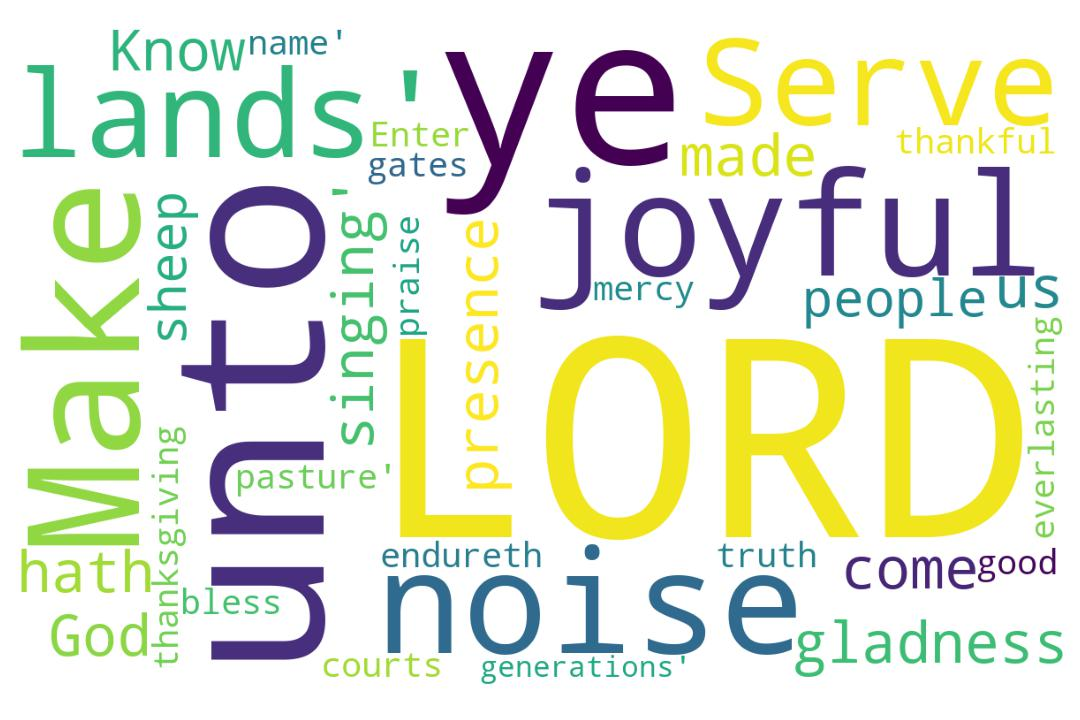
\includegraphics[width=\linewidth]{19OT-Psalms/Psalm100-WordCloud.jpg}
  \caption{Psalm 100 Word Cloud}
  \label{fig:Psalm 100 word Cloud}
\end{figure}


\marginpar{\scriptsize \centering \fcolorbox{bone}{lime}{\textbf{BECAUSE GOD IS GOOD}}\\ (Psalm 100:1-5)

\begin{compactenum}[I.][8]
    \item The \textbf{Geography} of Praise \index[scripture]{Psalms!Psa 100:01} (Psa 100:1)
    \item The \textbf{Gladness} of Praise \index[scripture]{Psalms!Psa 100:02} (Psa 100:2)
    \item Like \textbf{Grazing} Sheep \index[scripture]{Psalms!Psa 100:03} (Psa 100:3)
    \item The \textbf{Gates} of Thanksgiving \index[scripture]{Psalms!Psa 100:04} (Psa 100:4)
    \item The \textbf{Gladness} \index[scripture]{Psalms!Psa 100:02} (Psa 100:2)
    \item The \textbf{Gratitude} \index[scripture]{Psalms!Psa 100:02} (Psa 100:2)
    \item All \textbf{Generations} \index[scripture]{Psalms!Psa 100:05} (Psa 100:5)
    \item Because He is \textbf{Good} \index[scripture]{Psalms!Psa 100:05} (Psa 100:5)
\end{compactenum}}




\footnote{\textcolor[rgb]{0.00,0.25,0.00}{\hyperlink{TOC}{Return to end of Table of Contents.}}}\footnote{\href{https://audiobible.com/bible/psalms_100.html}{\textcolor[cmyk]{0.99998,1,0,0}{Psalm 100 Audio}}}\textcolor[cmyk]{0.99998,1,0,0}{A Psalm of praise.}\\
\\
\textcolor[cmyk]{0.99998,1,0,0}{Make a joyful noise unto the LORD, \fcolorbox{bone}{lime}{all ye lands}.}
[2] \textcolor[cmyk]{0.99998,1,0,0}{Serve the LORD with \fcolorbox{bone}{lime}{gladness}: come before his presence with singing.}
[3] \textcolor[cmyk]{0.99998,1,0,0}{Know ye that the LORD he \emph{is} God: \emph{it} \emph{is} he \emph{that} hath made us, and not we ourselves; \emph{we} \emph{are} his people, and the \fcolorbox{bone}{lime}{sheep of his pasture}.}
[4] \textcolor[cmyk]{0.99998,1,0,0}{Enter into his \fcolorbox{bone}{lime}{gates with thanksgiving}, \emph{and} into his courts with praise: be thankful unto him, \emph{and} bless his name.}
[5] \textcolor[cmyk]{0.99998,1,0,0}{For the LORD \emph{is} \fcolorbox{bone}{lime}{good}; his mercy \emph{is} everlasting; and his truth \emph{endureth} to all \fcolorbox{bone}{lime}{generations}.}
\index[NWIV]{10!Psalm!Psa 100:1}\index[AWIP]{Make!Psalm!Psa 100:1}\index[AWIP]{a!Psalm!Psa 100:1}\index[AWIP]{joyful!Psalm!Psa 100:1}\index[AWIP]{noise!Psalm!Psa 100:1}\index[AWIP]{unto!Psalm!Psa 100:1}\index[AWIP]{the!Psalm!Psa 100:1}\index[AWIP]{LORD!Psalm!Psa 100:1}\index[AWIP]{all!Psalm!Psa 100:1}\index[AWIP]{ye!Psalm!Psa 100:1}\index[AWIP]{lands!Psalm!Psa 100:1}

\index[NWIV]{11!Psalm!Psa 100:2}\index[AWIP]{Serve!Psalm!Psa 100:2}\index[AWIP]{the!Psalm!Psa 100:2}\index[AWIP]{LORD!Psalm!Psa 100:2}\index[AWIP]{with!Psalm!Psa 100:2}\index[AWIP]{with!Psalm!Psa 100:2 (2)}\index[AWIP]{gladness!Psalm!Psa 100:2}\index[AWIP]{come!Psalm!Psa 100:2}\index[AWIP]{before!Psalm!Psa 100:2}\index[AWIP]{his!Psalm!Psa 100:2}\index[AWIP]{presence!Psalm!Psa 100:2}\index[AWIP]{singing!Psalm!Psa 100:2}

\index[NWIV]{29!Psalm!Psa 100:3}\index[AWIP]{Know!Psalm!Psa 100:3}\index[AWIP]{ye!Psalm!Psa 100:3}\index[AWIP]{that!Psalm!Psa 100:3}\index[AWIP]{the!Psalm!Psa 100:3}\index[AWIP]{the!Psalm!Psa 100:3 (2)}\index[AWIP]{LORD!Psalm!Psa 100:3}\index[AWIP]{he!Psalm!Psa 100:3}\index[AWIP]{he!Psalm!Psa 100:3 (2)}\index[AWIP]{\emph{is}!Psalm!Psa 100:3}\index[AWIP]{\emph{is}!Psalm!Psa 100:3 (2)}\index[AWIP]{God!Psalm!Psa 100:3}\index[AWIP]{\emph{it}!Psalm!Psa 100:3}\index[AWIP]{\emph{that}!Psalm!Psa 100:3}\index[AWIP]{hath!Psalm!Psa 100:3}\index[AWIP]{made!Psalm!Psa 100:3}\index[AWIP]{us!Psalm!Psa 100:3}\index[AWIP]{and!Psalm!Psa 100:3}\index[AWIP]{and!Psalm!Psa 100:3 (2)}\index[AWIP]{not!Psalm!Psa 100:3}\index[AWIP]{we!Psalm!Psa 100:3}\index[AWIP]{ourselves!Psalm!Psa 100:3}\index[AWIP]{\emph{we}!Psalm!Psa 100:3}\index[AWIP]{\emph{are}!Psalm!Psa 100:3}\index[AWIP]{his!Psalm!Psa 100:3}\index[AWIP]{his!Psalm!Psa 100:3 (2)}\index[AWIP]{people!Psalm!Psa 100:3}\index[AWIP]{sheep!Psalm!Psa 100:3}\index[AWIP]{of!Psalm!Psa 100:3}\index[AWIP]{pasture!Psalm!Psa 100:3}\index[AWIP]{\emph{is}!Psalm!Psa 100:3}\index[AWIP]{\emph{is}!Psalm!Psa 100:3 (2)}\index[AWIP]{\emph{it}!Psalm!Psa 100:3}\index[AWIP]{\emph{that}!Psalm!Psa 100:3}\index[AWIP]{\emph{we}!Psalm!Psa 100:3}\index[AWIP]{\emph{are}!Psalm!Psa 100:3}

\index[NWIV]{20!Psalm!Psa 100:4}\index[AWIP]{Enter!Psalm!Psa 100:4}\index[AWIP]{into!Psalm!Psa 100:4}\index[AWIP]{into!Psalm!Psa 100:4 (2)}\index[AWIP]{his!Psalm!Psa 100:4}\index[AWIP]{his!Psalm!Psa 100:4 (2)}\index[AWIP]{his!Psalm!Psa 100:4 (3)}\index[AWIP]{gates!Psalm!Psa 100:4}\index[AWIP]{with!Psalm!Psa 100:4}\index[AWIP]{with!Psalm!Psa 100:4 (2)}\index[AWIP]{thanksgiving!Psalm!Psa 100:4}\index[AWIP]{\emph{and}!Psalm!Psa 100:4}\index[AWIP]{\emph{and}!Psalm!Psa 100:4 (2)}\index[AWIP]{courts!Psalm!Psa 100:4}\index[AWIP]{praise!Psalm!Psa 100:4}\index[AWIP]{be!Psalm!Psa 100:4}\index[AWIP]{thankful!Psalm!Psa 100:4}\index[AWIP]{unto!Psalm!Psa 100:4}\index[AWIP]{him!Psalm!Psa 100:4}\index[AWIP]{bless!Psalm!Psa 100:4}\index[AWIP]{name!Psalm!Psa 100:4}\index[AWIP]{\emph{and}!Psalm!Psa 100:4}\index[AWIP]{\emph{and}!Psalm!Psa 100:4 (2)}

\index[NWIV]{16!Psalm!Psa 100:5}\index[AWIP]{For!Psalm!Psa 100:5}\index[AWIP]{the!Psalm!Psa 100:5}\index[AWIP]{LORD!Psalm!Psa 100:5}\index[AWIP]{\emph{is}!Psalm!Psa 100:5}\index[AWIP]{\emph{is}!Psalm!Psa 100:5 (2)}\index[AWIP]{good!Psalm!Psa 100:5}\index[AWIP]{his!Psalm!Psa 100:5}\index[AWIP]{his!Psalm!Psa 100:5 (2)}\index[AWIP]{mercy!Psalm!Psa 100:5}\index[AWIP]{everlasting!Psalm!Psa 100:5}\index[AWIP]{and!Psalm!Psa 100:5}\index[AWIP]{truth!Psalm!Psa 100:5}\index[AWIP]{\emph{endureth}!Psalm!Psa 100:5}\index[AWIP]{to!Psalm!Psa 100:5}\index[AWIP]{all!Psalm!Psa 100:5}\index[AWIP]{generations!Psalm!Psa 100:5}\index[AWIP]{\emph{is}!Psalm!Psa 100:5}\index[AWIP]{\emph{is}!Psalm!Psa 100:5 (2)}\index[AWIP]{\emph{endureth}!Psalm!Psa 100:5}


\section{Psalm 100 Outlines}

\subsection{My Outlines}

\subsubsection{Because God is Good}

\index[speaker]{Keith Anthony!Psalm 100 (Because God is Good)}
\index[series]{Psalms (Keith Anthony)!Psalm 100 (Because God is Good)}
\index[date]{2017/09/02!Psalm 100 (Because God is Good) (Keith Anthony)}

\begin{compactenum}[I.]
    \item The \textbf{Geography} of Praise \index[scripture]{Psalms!Psa 100:01} (Psa 100:1)
    \item The \textbf{Gladness} of Praise \index[scripture]{Psalms!Psa 100:02} (Psa 100:2)
    \item Like \textbf{Grazing} Sheep \index[scripture]{Psalms!Psa 100:03} (Psa 100:3)
    \item The \textbf{Gates} of Thanksgiving \index[scripture]{Psalms!Psa 100:04} (Psa 100:4)
    \item The \textbf{Gratitude} \index[scripture]{Psalms!Psa 100:02} (Psa 100:2)
    \item All \textbf{Generations} \index[scripture]{Psalms!Psa 100:05} (Psa 100:5)
    \item Because He is \textbf{Good} \index[scripture]{Psalms!Psa 100:05} (Psa 100:5)
\end{compactenum}


%\subsection{Outlines from Others}


\section{Psalm 100 Comments}




\subsection{Psalm 100 Repeated Phrases}


%%%%%%%%%%
%%%%%%%%%%
\normalsize
 
\begin{center}
\begin{longtable}{|p{3.0in}|p{0.5in}|}
\caption[Psalm 100 Repeated Phrases]{Psalm 100 Repeated Phrases}\label{table:Repeated Phrases Psalm 100} \\
\hline \multicolumn{1}{|c|}{\textbf{Phrase}} & \multicolumn{1}{c|}{\textbf{Frequency}} \\ \hline 
\endfirsthead
 
\multicolumn{2}{c}
{{\bfseries \tablename\ \thetable{} -- continued from previous page}} \\  
\hline \multicolumn{1}{|c|}{\textbf{Phrase}} & \multicolumn{1}{c|}{\textbf{Frequency}} \\ \hline 
\endhead
 
\hline \multicolumn{2}{c}{{ }} \\ \hline
\endfoot 
the LORD & 4\\ \hline 
\end{longtable}
\end{center}



%%%%%%%%%%
%%%%%%%%%%



\section{Psalm 100 Statistics}

%%%%%%%%%%%%%%%%%%%%%%%%%%%
%%%%% Word Statistics
%%%%%%%%%%%%%%%%%%%%%%%%%%


\normalsize



\subsection{Chapter Word Statistics}


%%%%%%%%%%
%%%%%%%%%%
 
\begin{center}
\begin{longtable}{l|c|c|c|c}
\caption[Stats for Psalm 100]{Stats for Psalm 100} \label{table:Stats for Psalm 100} \\ 
\hline \multicolumn{1}{|c|}{\textbf{Verse(s)}} & \multicolumn{1}{|c|}{\textbf{Count}} & \multicolumn{1}{|c|}{\textbf{Unique}} & \multicolumn{1}{|c|}{\textbf{Italics}} & \multicolumn{1}{|c|}{\textbf{Uniq Italic}}  \\ \hline 
\endfirsthead
 
\multicolumn{5}{c}
{{\bfseries \tablename\ \thetable{} -- continued from previous page}} \\  
\hline \multicolumn{1}{|c|}{\textbf{Verse(s)}} & \multicolumn{1}{|c|}{\textbf{Count}} & \multicolumn{1}{|c|}{\textbf{Unique}} & \multicolumn{1}{|c|}{\textbf{Italics}} & \multicolumn{1}{|c|}{\textbf{Uniq Italic}}  \\ \hline 
\endhead
 
\hline \multicolumn{5}{|r|}{{Continued if needed}} \\ \hline
\endfoot 
1 & 10 & 10 & 0 & 0\\ \hline
2 & 11 & 10 & 0 & 0\\ \hline
3 & 29 & 24 & 6 & 5\\ \hline
4 & 20 & 15 & 2 & 1\\ \hline
5 & 16 & 14 & 3 & 2\\ \hline
\hline \hline
Total & 86 & 58 & 11 & 7



\end{longtable}
\end{center}

%%%%%%%%%%
%%%%%%%%%%
 
\subsection{Words by Frequency}

\begin{center}
\begin{longtable}{l|r}
\caption[Word Frequencies in Psalm 100]{Word Frequencies in Psalm 100} \label{table:WordsIn-Psalm-100} \\ 
\hline \multicolumn{1}{|c|}{\textbf{Word}} & \multicolumn{1}{c|}{\textbf{Frequency}} \\ \hline 
\endfirsthead
 
\multicolumn{2}{c}
{{\bfseries \tablename\ \thetable{} -- continued from previous page}} \\ 
\hline \multicolumn{1}{|c|}{\textbf{Word}} & \multicolumn{1}{c|}{\textbf{Frequency}} \\ \hline 
\endhead
 
\hline \multicolumn{2}{|r|}{{Continued if needed}} \\ \hline
\endfoot
 
\hline \hline
\endlastfoot
his & 8 \\ \hline
the & 5 \\ \hline
LORD & 4 \\ \hline
with & 4 \\ \hline
\emph{is} & 4 \\ \hline
and & 3 \\ \hline
unto & 2 \\ \hline
all & 2 \\ \hline
ye & 2 \\ \hline
he & 2 \\ \hline
into & 2 \\ \hline
\emph{and} & 2 \\ \hline
Make & 1 \\ \hline
a & 1 \\ \hline
joyful & 1 \\ \hline
noise & 1 \\ \hline
lands & 1 \\ \hline
Serve & 1 \\ \hline
gladness & 1 \\ \hline
come & 1 \\ \hline
before & 1 \\ \hline
presence & 1 \\ \hline
singing & 1 \\ \hline
Know & 1 \\ \hline
that & 1 \\ \hline
God & 1 \\ \hline
\emph{it} & 1 \\ \hline
\emph{that} & 1 \\ \hline
hath & 1 \\ \hline
made & 1 \\ \hline
us & 1 \\ \hline
not & 1 \\ \hline
we & 1 \\ \hline
ourselves & 1 \\ \hline
\emph{we} & 1 \\ \hline
\emph{are} & 1 \\ \hline
people & 1 \\ \hline
sheep & 1 \\ \hline
of & 1 \\ \hline
pasture & 1 \\ \hline
Enter & 1 \\ \hline
gates & 1 \\ \hline
thanksgiving & 1 \\ \hline
courts & 1 \\ \hline
praise & 1 \\ \hline
be & 1 \\ \hline
thankful & 1 \\ \hline
him & 1 \\ \hline
bless & 1 \\ \hline
name & 1 \\ \hline
For & 1 \\ \hline
good & 1 \\ \hline
mercy & 1 \\ \hline
everlasting & 1 \\ \hline
truth & 1 \\ \hline
\emph{endureth} & 1 \\ \hline
to & 1 \\ \hline
generations & 1 \\ \hline
\end{longtable}
\end{center}



\normalsize



\subsection{Words Alphabetically}

\begin{center}
\begin{longtable}{l|r}
\caption[Word Alphabetically in Psalm 100]{Word Alphabetically in Psalm 100} \label{table:WordsIn-Psalm-100} \\ 
\hline \multicolumn{1}{|c|}{\textbf{Word}} & \multicolumn{1}{c|}{\textbf{Frequency}} \\ \hline 
\endfirsthead
 
\multicolumn{2}{c}
{{\bfseries \tablename\ \thetable{} -- continued from previous page}} \\ 
\hline \multicolumn{1}{|c|}{\textbf{Word}} & \multicolumn{1}{c|}{\textbf{Frequency}} \\ \hline 
\endhead
 
\hline \multicolumn{2}{|r|}{{Continued if needed}} \\ \hline
\endfoot
 
\hline \hline
\endlastfoot
Enter & 1 \\ \hline
For & 1 \\ \hline
God & 1 \\ \hline
Know & 1 \\ \hline
LORD & 4 \\ \hline
Make & 1 \\ \hline
Serve & 1 \\ \hline
\emph{and} & 2 \\ \hline
\emph{are} & 1 \\ \hline
\emph{endureth} & 1 \\ \hline
\emph{is} & 4 \\ \hline
\emph{it} & 1 \\ \hline
\emph{that} & 1 \\ \hline
\emph{we} & 1 \\ \hline
a & 1 \\ \hline
all & 2 \\ \hline
and & 3 \\ \hline
be & 1 \\ \hline
before & 1 \\ \hline
bless & 1 \\ \hline
come & 1 \\ \hline
courts & 1 \\ \hline
everlasting & 1 \\ \hline
gates & 1 \\ \hline
generations & 1 \\ \hline
gladness & 1 \\ \hline
good & 1 \\ \hline
hath & 1 \\ \hline
he & 2 \\ \hline
him & 1 \\ \hline
his & 8 \\ \hline
into & 2 \\ \hline
joyful & 1 \\ \hline
lands & 1 \\ \hline
made & 1 \\ \hline
mercy & 1 \\ \hline
name & 1 \\ \hline
noise & 1 \\ \hline
not & 1 \\ \hline
of & 1 \\ \hline
ourselves & 1 \\ \hline
pasture & 1 \\ \hline
people & 1 \\ \hline
praise & 1 \\ \hline
presence & 1 \\ \hline
sheep & 1 \\ \hline
singing & 1 \\ \hline
thankful & 1 \\ \hline
thanksgiving & 1 \\ \hline
that & 1 \\ \hline
the & 5 \\ \hline
to & 1 \\ \hline
truth & 1 \\ \hline
unto & 2 \\ \hline
us & 1 \\ \hline
we & 1 \\ \hline
with & 4 \\ \hline
ye & 2 \\ \hline
\end{longtable}
\end{center}



\normalsize



\subsection{Word Lengths in Chapter}
\normalsize
\begin{longtable}{l|p{3.75in}}
\caption[Words by Length in Psalm 100]{Words by Length in Psalm 100} \label{table:WordsIn-Psalm-100} \\ 
\hline \multicolumn{1}{|c|}{\textbf{Length}} & \multicolumn{1}{c|}{\textbf{Words}} \\ \hline 
\endfirsthead
 
\multicolumn{2}{c}
{{\bfseries \tablename\ \thetable{} -- continued from previous page}} \\ 
\hline \multicolumn{1}{|c|}{\textbf{Length}} & \multicolumn{1}{c|}{\textbf{Words}} \\ \hline 
\endhead
 
\hline \multicolumn{2}{|r|}{{Continued if needed}} \\ \hline
\endfoot
 
\hline \hline
\endlastfoot
1 & a \\ \hline
2 & ye, he, \emph{is}, \emph{it}, us, we, \emph{we}, of, be, to \\ \hline
3 & the, all, his, God, and, not, \emph{are}, \emph{and}, him, For \\ \hline
4 & Make, unto, LORD, with, come, Know, that, \emph{that}, hath, made, into, name, good \\ \hline
5 & noise, lands, Serve, sheep, Enter, gates, bless, mercy, truth \\ \hline
6 & joyful, before, people, courts, praise \\ \hline
7 & singing, pasture \\ \hline
8 & gladness, presence, thankful, \emph{endureth} \\ \hline
9 & ourselves \\ \hline
11 & everlasting, generations \\ \hline
12 & thanksgiving \\ \hline
\end{longtable}






%%%%%%%%%%
%%%%%%%%%%
\input{19OT-Psalms/Psalm100-Devotionals}

\chapter{Proverb 10}

\begin{figure}
  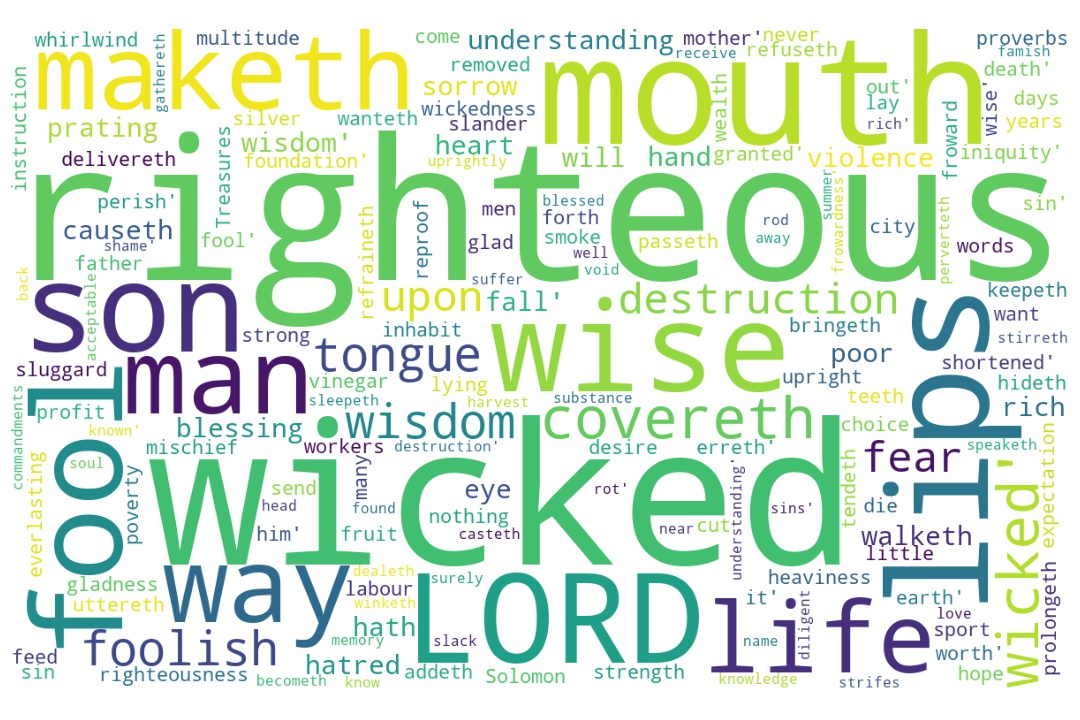
\includegraphics[width=\linewidth]{20OT-Proverbs/Proverb10-WordCloud.jpg}
  \caption{Proverb 10 Word Cloud}
  \label{fig:Proverb 10 Word Cloud}
\end{figure}

\marginpar{\scriptsize \centering\fcolorbox{bone}{lime}{\textbf{THE RIGHTEOUS \& WICKED}}\\ (Proverb 10:1-32)
\begin{compactenum}[I.][8]
	\item \textbf{Shame to the Lazy}  \index[scripture]{Proverbs!Pro 10:05} (Pro 10:5)
	\item \textbf{Sure Footing for the Upright}  \index[scripture]{Proverbs!Pro 10:09} (Pro 10:9)
	\item \textbf{Strife to the Hateful}  \index[scripture]{Proverbs!Pro 10:12} (Pro 10:12)
	\item More \textbf{Sin for the Wicked}  \index[scripture]{Proverbs!Pro 10:16} (Pro 10:16)
	\item \textbf{Sustenance form the Righteous}  \index[scripture]{Proverbs!Pro 10:21} (Pro 10:21)
	\item \textbf{Stinging Eyes to the Sluggard}  \index[scripture]{Proverbs!Pro 10:26} (Pro 10:26)
	\item \textbf{Strength to the Upright} \index[scripture]{Proverbs!Pro 10:29} (Pro 10:29)
\end{compactenum}}

\marginpar{\scriptsize \centering\fcolorbox{bone}{yellow}{\textbf{7 THINGS OF LIFE}}\\ (Proverb 10:1-32)
    \begin{compactenum}[I.][8]
	\item The \textbf{Well} of Life \index[scripture]{Proverbs!Pro 10:11} (Pro 10:11)
	
	\item A \textbf{Wellspring} of Life \index[scripture]{Proverbs!Pro 16:22} \index[scripture]{Proverbs!Pro 18:4} (Pro 16:22, 18:4)
	
	\item The \textbf{way} of Life \index[scripture]{Pro!Pro 06:23} \index[scripture]{Pro!Pro 10:17} \index[scripture]{Pro!Pro 15:24} \index[scripture]{Jer!Jer 21:8} (Pro 6:23, 10:17, 15:24, Jer 21:8)

	\item The \textbf{ways} of Life \index[scripture]{Acts!Acts 02:28} (Acts 2:28)
	
	\item The \textbf{water} of Life \index[scripture]{Rev!Rev 21:06} \index[scripture]{Rev!Rev 22:01} \index[scripture]{Rev!Rev 22:17}  (Rev 21:6, 22:1, 22:17)
	
	\item The \textbf{word} of Life \index[scripture]{Phil!Phil 02:16} (Phil 2:16)
	
	\item The \textbf{Word} of Life \index[scripture]{1Jn!1Jn 1:1}  (1 John 1:1)
\end{compactenum}}

\footnote{\textcolor[cmyk]{0.99998,1,0,0}{\hyperlink{TOC}{Return to end of Table of Contents.}}}\footnote{\href{https://audiobible.com/bible/proverbs_10.html}{\textcolor[cmyk]{0.99998,1,0,0}{Proverbs Audio}}}\textcolor[cmyk]{0.99998,1,0,0}{The proverbs of Solomon. A wise son maketh a glad father: but a foolish son \emph{is} the heaviness of his mother.}
[2] \textcolor[cmyk]{0.99998,1,0,0}{Treasures of wickedness profit nothing: but \fcolorbox{bone}{MYGOLD}{righteousness} delivereth from death.}
[3] \textcolor[cmyk]{0.99998,1,0,0}{The LORD will not suffer the soul of the righteous to famish: but he casteth away the substance of the wicked.}\footnote{\textbf{Psalm 37:25} - I have been young, and now am old; yet have I not seen the righteous forsaken, nor his seed begging bread.}
[4] \textcolor[cmyk]{0.99998,1,0,0}{He becometh poor that dealeth \emph{with} a slack hand: but the hand of the diligent maketh rich.}
[5] \textcolor[cmyk]{0.99998,1,0,0}{He that gathereth in summer \emph{is} a wise son: \emph{but} he that sleepeth in harvest \emph{is} a son that causeth \fcolorbox{bone}{lime}{shame}.}
[6] \textcolor[cmyk]{0.99998,1,0,0}{Blessings \emph{are} upon the head of the just: but violence covereth the mouth of the wicked.}
[7] \textcolor[cmyk]{0.99998,1,0,0}{The memory of the just \emph{is} blessed: but the name of the wicked shall rot.}
[8] \textcolor[cmyk]{0.99998,1,0,0}{Thewise in heart will receive commandments: but a prating fool shall fall.}
[9] \textcolor[cmyk]{0.99998,1,0,0}{He that walketh uprightly walketh \fcolorbox{bone}{lime}{surely}: but he that perverteth his ways shall be known.}
[10] \textcolor[cmyk]{0.99998,1,0,0}{He that winketh with the eye causeth sorrow: but a prating fool shall fall.}\footnote{\textbf{Proverbs 6:13} - He winketh with his eyes, he speaketh with his feet, he teacheth with his fingers;} 
[11] \textcolor[cmyk]{0.99998,1,0,0}{The mouth of a righteous \emph{man} \emph{is} a well of life: but violence covereth the mouth of the wicked.}\footnote{\textbf{Proverb 16:22} - Understanding is a wellspring of life unto him that hath it: but the instruction of fools is folly.}
[12] \textcolor[cmyk]{0.99998,1,0,0}{Hatred stirreth up \fcolorbox{bone}{lime}{strifes}: but love covereth all sins.}
[13] \textcolor[cmyk]{0.99998,1,0,0}{In  the lips of him that hath \fcolorbox{bone}{MYGOLD}{understanding} wisdom is found: but a rod \emph{is} for the back of him that is void of \fcolorbox{bone}{MYGOLD}{understanding}.}
[14] \textcolor[cmyk]{0.99998,1,0,0}{Wise  \emph{men} lay up knowledge: but the mouth of the foolish \emph{is} near destruction.}
[15] \textcolor[cmyk]{0.99998,1,0,0}{The  rich man's wealth \emph{is} his strong city: the destruction of the poor \emph{is} their poverty.}
[16] \textcolor[cmyk]{0.99998,1,0,0}{The  labour of the righteous \emph{tendeth} to life: the fruit of the wicked \fcolorbox{bone}{lime}{to sin}.}
[17] \textcolor[cmyk]{0.99998,1,0,0}{He  \emph{is} \emph{in} the way of life that keepeth instruction: but he that refuseth reproof erreth.}
[18] \textcolor[cmyk]{0.99998,1,0,0}{He  that hideth hatred \emph{with} lying lips, and he that uttereth a slander, \emph{is} a fool.}
[19] \textcolor[cmyk]{0.99998,1,0,0}{In  the multitude of words there wanteth not sin: but he that refraineth his lips \emph{is} wise.}
[20] \textcolor[cmyk]{0.99998,1,0,0}{The tongue of the just \emph{is} \emph{as} choice silver: the heart of the wicked \emph{is} little worth.}
[21] \textcolor[cmyk]{0.99998,1,0,0}{The lips of the righteous \fcolorbox{bone}{lime}{feed many}: but fools die for want of wisdom.}
[22] \textcolor[cmyk]{0.99998,1,0,0}{The blessing of the LORD, it maketh rich, and he addeth no sorrow with it.}
[23] \textcolor[cmyk]{0.99998,1,0,0}{\emph{It} \emph{is} as sport to a fool to do mischief: but a man of \fcolorbox{bone}{MYGOLD}{understanding} hath wisdom.}
[24] \textcolor[cmyk]{0.99998,1,0,0}{The fear of the wicked, it shall come upon him: but the desire of the righteous shall be granted.}
[25] \textcolor[cmyk]{0.99998,1,0,0}{As the whirlwind passeth, so \emph{is} the wicked no \emph{more}: but the righteous \emph{is} an everlasting foundation.}
[26] \textcolor[cmyk]{0.99998,1,0,0}{As vinegar to the teeth, and as \fcolorbox{bone}{lime}{smoke to the eyes}, so \emph{is} the sluggard to them that send him.}
[27] \textcolor[cmyk]{0.99998,1,0,0}{The fear of the LORD prolongeth days: but the years of the wicked shall be shortened.}
[28] \textcolor[cmyk]{0.99998,1,0,0}{The hope of the righteous \emph{shall} \emph{be} gladness: but the expectation of the wicked shall perish.}
[29] \textcolor[cmyk]{0.99998,1,0,0}{The way of the LORD \emph{is} \fcolorbox{bone}{lime}{strength to the upright}: but destruction \emph{shall} \emph{be} to the workers of iniquity.}
[30] \textcolor[cmyk]{0.99998,1,0,0}{The righteous shall never be removed: but the wicked shall not inhabit the earth.}
[31] \textcolor[cmyk]{0.99998,1,0,0}{The mouth of the just bringeth forth wisdom: but the froward tongue shall be cut out.}
[32] \textcolor[cmyk]{0.99998,1,0,0}{The lips of the righteous know what is acceptable: but the mouth of the wicked \emph{speaketh} frowardness.}


\index[NWIV]{21!Proverbs!Pro 10:1}\index[AWIP]{The!Proverbs!Pro 10:1}\index[AWIP]{proverbs!Proverbs!Pro 10:1}\index[AWIP]{of!Proverbs!Pro 10:1}\index[AWIP]{of!Proverbs!Pro 10:1 (2)}\index[AWIP]{Solomon!Proverbs!Pro 10:1}\index[AWIP]{A!Proverbs!Pro 10:1}\index[AWIP]{wise!Proverbs!Pro 10:1}\index[AWIP]{son!Proverbs!Pro 10:1}\index[AWIP]{son!Proverbs!Pro 10:1 (2)}\index[AWIP]{maketh!Proverbs!Pro 10:1}\index[AWIP]{a!Proverbs!Pro 10:1}\index[AWIP]{a!Proverbs!Pro 10:1 (2)}\index[AWIP]{glad!Proverbs!Pro 10:1}\index[AWIP]{father!Proverbs!Pro 10:1}\index[AWIP]{but!Proverbs!Pro 10:1}\index[AWIP]{foolish!Proverbs!Pro 10:1}\index[AWIP]{\emph{is}!Proverbs!Pro 10:1}\index[AWIP]{the!Proverbs!Pro 10:1}\index[AWIP]{heaviness!Proverbs!Pro 10:1}\index[AWIP]{his!Proverbs!Pro 10:1}\index[AWIP]{mother!Proverbs!Pro 10:1}\index[AWIP]{\emph{is}!Proverbs!Pro 10:1}

\index[NWIV]{10!Proverbs!Pro 10:2}\index[AWIP]{Treasures!Proverbs!Pro 10:2}\index[AWIP]{of!Proverbs!Pro 10:2}\index[AWIP]{wickedness!Proverbs!Pro 10:2}\index[AWIP]{profit!Proverbs!Pro 10:2}\index[AWIP]{nothing!Proverbs!Pro 10:2}\index[AWIP]{but!Proverbs!Pro 10:2}\index[AWIP]{righteousness!Proverbs!Pro 10:2}\index[AWIP]{delivereth!Proverbs!Pro 10:2}\index[AWIP]{from!Proverbs!Pro 10:2}\index[AWIP]{death!Proverbs!Pro 10:2}

\index[NWIV]{21!Proverbs!Pro 10:3}\index[AWIP]{The!Proverbs!Pro 10:3}\index[AWIP]{LORD!Proverbs!Pro 10:3}\index[AWIP]{will!Proverbs!Pro 10:3}\index[AWIP]{not!Proverbs!Pro 10:3}\index[AWIP]{suffer!Proverbs!Pro 10:3}\index[AWIP]{the!Proverbs!Pro 10:3}\index[AWIP]{the!Proverbs!Pro 10:3 (2)}\index[AWIP]{the!Proverbs!Pro 10:3 (3)}\index[AWIP]{the!Proverbs!Pro 10:3 (4)}\index[AWIP]{soul!Proverbs!Pro 10:3}\index[AWIP]{of!Proverbs!Pro 10:3}\index[AWIP]{of!Proverbs!Pro 10:3 (2)}\index[AWIP]{righteous!Proverbs!Pro 10:3}\index[AWIP]{to!Proverbs!Pro 10:3}\index[AWIP]{famish!Proverbs!Pro 10:3}\index[AWIP]{but!Proverbs!Pro 10:3}\index[AWIP]{he!Proverbs!Pro 10:3}\index[AWIP]{casteth!Proverbs!Pro 10:3}\index[AWIP]{away!Proverbs!Pro 10:3}\index[AWIP]{substance!Proverbs!Pro 10:3}\index[AWIP]{wicked!Proverbs!Pro 10:3}

\index[NWIV]{17!Proverbs!Pro 10:4}\index[AWIP]{He!Proverbs!Pro 10:4}\index[AWIP]{becometh!Proverbs!Pro 10:4}\index[AWIP]{poor!Proverbs!Pro 10:4}\index[AWIP]{that!Proverbs!Pro 10:4}\index[AWIP]{dealeth!Proverbs!Pro 10:4}\index[AWIP]{\emph{with}!Proverbs!Pro 10:4}\index[AWIP]{a!Proverbs!Pro 10:4}\index[AWIP]{slack!Proverbs!Pro 10:4}\index[AWIP]{hand!Proverbs!Pro 10:4}\index[AWIP]{hand!Proverbs!Pro 10:4 (2)}\index[AWIP]{but!Proverbs!Pro 10:4}\index[AWIP]{the!Proverbs!Pro 10:4}\index[AWIP]{the!Proverbs!Pro 10:4 (2)}\index[AWIP]{of!Proverbs!Pro 10:4}\index[AWIP]{diligent!Proverbs!Pro 10:4}\index[AWIP]{maketh!Proverbs!Pro 10:4}\index[AWIP]{rich!Proverbs!Pro 10:4}\index[AWIP]{\emph{with}!Proverbs!Pro 10:4}

\index[NWIV]{21!Proverbs!Pro 10:5}\index[AWIP]{He!Proverbs!Pro 10:5}\index[AWIP]{that!Proverbs!Pro 10:5}\index[AWIP]{that!Proverbs!Pro 10:5 (2)}\index[AWIP]{that!Proverbs!Pro 10:5 (3)}\index[AWIP]{gathereth!Proverbs!Pro 10:5}\index[AWIP]{in!Proverbs!Pro 10:5}\index[AWIP]{in!Proverbs!Pro 10:5 (2)}\index[AWIP]{summer!Proverbs!Pro 10:5}\index[AWIP]{\emph{is}!Proverbs!Pro 10:5}\index[AWIP]{\emph{is}!Proverbs!Pro 10:5 (2)}\index[AWIP]{a!Proverbs!Pro 10:5}\index[AWIP]{a!Proverbs!Pro 10:5 (2)}\index[AWIP]{wise!Proverbs!Pro 10:5}\index[AWIP]{son!Proverbs!Pro 10:5}\index[AWIP]{son!Proverbs!Pro 10:5 (2)}\index[AWIP]{\emph{but}!Proverbs!Pro 10:5}\index[AWIP]{he!Proverbs!Pro 10:5}\index[AWIP]{sleepeth!Proverbs!Pro 10:5}\index[AWIP]{harvest!Proverbs!Pro 10:5}\index[AWIP]{causeth!Proverbs!Pro 10:5}\index[AWIP]{shame!Proverbs!Pro 10:5}\index[AWIP]{\emph{is}!Proverbs!Pro 10:5}\index[AWIP]{\emph{is}!Proverbs!Pro 10:5 (2)}\index[AWIP]{\emph{but}!Proverbs!Pro 10:5}

\index[NWIV]{16!Proverbs!Pro 10:6}\index[AWIP]{Blessings!Proverbs!Pro 10:6}\index[AWIP]{\emph{are}!Proverbs!Pro 10:6}\index[AWIP]{upon!Proverbs!Pro 10:6}\index[AWIP]{the!Proverbs!Pro 10:6}\index[AWIP]{the!Proverbs!Pro 10:6 (2)}\index[AWIP]{the!Proverbs!Pro 10:6 (3)}\index[AWIP]{the!Proverbs!Pro 10:6 (4)}\index[AWIP]{head!Proverbs!Pro 10:6}\index[AWIP]{of!Proverbs!Pro 10:6}\index[AWIP]{of!Proverbs!Pro 10:6 (2)}\index[AWIP]{just!Proverbs!Pro 10:6}\index[AWIP]{but!Proverbs!Pro 10:6}\index[AWIP]{violence!Proverbs!Pro 10:6}\index[AWIP]{covereth!Proverbs!Pro 10:6}\index[AWIP]{mouth!Proverbs!Pro 10:6}\index[AWIP]{wicked!Proverbs!Pro 10:6}\index[AWIP]{\emph{are}!Proverbs!Pro 10:6}

\index[NWIV]{15!Proverbs!Pro 10:7}\index[AWIP]{The!Proverbs!Pro 10:7}\index[AWIP]{memory!Proverbs!Pro 10:7}\index[AWIP]{of!Proverbs!Pro 10:7}\index[AWIP]{of!Proverbs!Pro 10:7 (2)}\index[AWIP]{the!Proverbs!Pro 10:7}\index[AWIP]{the!Proverbs!Pro 10:7 (2)}\index[AWIP]{the!Proverbs!Pro 10:7 (3)}\index[AWIP]{just!Proverbs!Pro 10:7}\index[AWIP]{\emph{is}!Proverbs!Pro 10:7}\index[AWIP]{blessed!Proverbs!Pro 10:7}\index[AWIP]{but!Proverbs!Pro 10:7}\index[AWIP]{name!Proverbs!Pro 10:7}\index[AWIP]{wicked!Proverbs!Pro 10:7}\index[AWIP]{shall!Proverbs!Pro 10:7}\index[AWIP]{rot!Proverbs!Pro 10:7}\index[AWIP]{\emph{is}!Proverbs!Pro 10:7}

\index[NWIV]{13!Proverbs!Pro 10:8}\index[AWIP]{The!Proverbs!Pro 10:8}\index[AWIP]{wise!Proverbs!Pro 10:8}\index[AWIP]{in!Proverbs!Pro 10:8}\index[AWIP]{heart!Proverbs!Pro 10:8}\index[AWIP]{will!Proverbs!Pro 10:8}\index[AWIP]{receive!Proverbs!Pro 10:8}\index[AWIP]{commandments!Proverbs!Pro 10:8}\index[AWIP]{but!Proverbs!Pro 10:8}\index[AWIP]{a!Proverbs!Pro 10:8}\index[AWIP]{prating!Proverbs!Pro 10:8}\index[AWIP]{fool!Proverbs!Pro 10:8}\index[AWIP]{shall!Proverbs!Pro 10:8}\index[AWIP]{fall!Proverbs!Pro 10:8}

\index[NWIV]{15!Proverbs!Pro 10:9}\index[AWIP]{He!Proverbs!Pro 10:9}\index[AWIP]{that!Proverbs!Pro 10:9}\index[AWIP]{that!Proverbs!Pro 10:9 (2)}\index[AWIP]{walketh!Proverbs!Pro 10:9}\index[AWIP]{walketh!Proverbs!Pro 10:9 (2)}\index[AWIP]{uprightly!Proverbs!Pro 10:9}\index[AWIP]{surely!Proverbs!Pro 10:9}\index[AWIP]{but!Proverbs!Pro 10:9}\index[AWIP]{he!Proverbs!Pro 10:9}\index[AWIP]{perverteth!Proverbs!Pro 10:9}\index[AWIP]{his!Proverbs!Pro 10:9}\index[AWIP]{ways!Proverbs!Pro 10:9}\index[AWIP]{shall!Proverbs!Pro 10:9}\index[AWIP]{be!Proverbs!Pro 10:9}\index[AWIP]{known!Proverbs!Pro 10:9}

\index[NWIV]{14!Proverbs!Pro 10:10}\index[AWIP]{He!Proverbs!Pro 10:10}\index[AWIP]{that!Proverbs!Pro 10:10}\index[AWIP]{winketh!Proverbs!Pro 10:10}\index[AWIP]{with!Proverbs!Pro 10:10}\index[AWIP]{the!Proverbs!Pro 10:10}\index[AWIP]{eye!Proverbs!Pro 10:10}\index[AWIP]{causeth!Proverbs!Pro 10:10}\index[AWIP]{sorrow!Proverbs!Pro 10:10}\index[AWIP]{but!Proverbs!Pro 10:10}\index[AWIP]{a!Proverbs!Pro 10:10}\index[AWIP]{prating!Proverbs!Pro 10:10}\index[AWIP]{fool!Proverbs!Pro 10:10}\index[AWIP]{shall!Proverbs!Pro 10:10}\index[AWIP]{fall!Proverbs!Pro 10:10}

\index[NWIV]{19!Proverbs!Pro 10:11}\index[AWIP]{The!Proverbs!Pro 10:11}\index[AWIP]{mouth!Proverbs!Pro 10:11}\index[AWIP]{mouth!Proverbs!Pro 10:11 (2)}\index[AWIP]{of!Proverbs!Pro 10:11}\index[AWIP]{of!Proverbs!Pro 10:11 (2)}\index[AWIP]{of!Proverbs!Pro 10:11 (3)}\index[AWIP]{a!Proverbs!Pro 10:11}\index[AWIP]{a!Proverbs!Pro 10:11 (2)}\index[AWIP]{righteous!Proverbs!Pro 10:11}\index[AWIP]{\emph{man}!Proverbs!Pro 10:11}\index[AWIP]{\emph{is}!Proverbs!Pro 10:11}\index[AWIP]{well!Proverbs!Pro 10:11}\index[AWIP]{life!Proverbs!Pro 10:11}\index[AWIP]{but!Proverbs!Pro 10:11}\index[AWIP]{violence!Proverbs!Pro 10:11}\index[AWIP]{covereth!Proverbs!Pro 10:11}\index[AWIP]{the!Proverbs!Pro 10:11}\index[AWIP]{the!Proverbs!Pro 10:11 (2)}\index[AWIP]{wicked!Proverbs!Pro 10:11}\index[AWIP]{\emph{man}!Proverbs!Pro 10:11}\index[AWIP]{\emph{is}!Proverbs!Pro 10:11}

\index[NWIV]{9!Proverbs!Pro 10:12}\index[AWIP]{Hatred!Proverbs!Pro 10:12}\index[AWIP]{stirreth!Proverbs!Pro 10:12}\index[AWIP]{up!Proverbs!Pro 10:12}\index[AWIP]{strifes!Proverbs!Pro 10:12}\index[AWIP]{but!Proverbs!Pro 10:12}\index[AWIP]{love!Proverbs!Pro 10:12}\index[AWIP]{covereth!Proverbs!Pro 10:12}\index[AWIP]{all!Proverbs!Pro 10:12}\index[AWIP]{sins!Proverbs!Pro 10:12}

\index[NWIV]{25!Proverbs!Pro 10:13}\index[AWIP]{In!Proverbs!Pro 10:13}\index[AWIP]{the!Proverbs!Pro 10:13}\index[AWIP]{the!Proverbs!Pro 10:13 (2)}\index[AWIP]{lips!Proverbs!Pro 10:13}\index[AWIP]{of!Proverbs!Pro 10:13}\index[AWIP]{of!Proverbs!Pro 10:13 (2)}\index[AWIP]{of!Proverbs!Pro 10:13 (3)}\index[AWIP]{him!Proverbs!Pro 10:13}\index[AWIP]{him!Proverbs!Pro 10:13 (2)}\index[AWIP]{that!Proverbs!Pro 10:13}\index[AWIP]{that!Proverbs!Pro 10:13 (2)}\index[AWIP]{hath!Proverbs!Pro 10:13}\index[AWIP]{understanding!Proverbs!Pro 10:13}\index[AWIP]{understanding!Proverbs!Pro 10:13 (2)}\index[AWIP]{wisdom!Proverbs!Pro 10:13}\index[AWIP]{is!Proverbs!Pro 10:13}\index[AWIP]{is!Proverbs!Pro 10:13 (2)}\index[AWIP]{found!Proverbs!Pro 10:13}\index[AWIP]{but!Proverbs!Pro 10:13}\index[AWIP]{a!Proverbs!Pro 10:13}\index[AWIP]{rod!Proverbs!Pro 10:13}\index[AWIP]{\emph{is}!Proverbs!Pro 10:13}\index[AWIP]{for!Proverbs!Pro 10:13}\index[AWIP]{back!Proverbs!Pro 10:13}\index[AWIP]{void!Proverbs!Pro 10:13}\index[AWIP]{\emph{is}!Proverbs!Pro 10:13}

\index[NWIV]{14!Proverbs!Pro 10:14}\index[AWIP]{Wise!Proverbs!Pro 10:14}\index[AWIP]{\emph{men}!Proverbs!Pro 10:14}\index[AWIP]{lay!Proverbs!Pro 10:14}\index[AWIP]{up!Proverbs!Pro 10:14}\index[AWIP]{knowledge!Proverbs!Pro 10:14}\index[AWIP]{but!Proverbs!Pro 10:14}\index[AWIP]{the!Proverbs!Pro 10:14}\index[AWIP]{the!Proverbs!Pro 10:14 (2)}\index[AWIP]{mouth!Proverbs!Pro 10:14}\index[AWIP]{of!Proverbs!Pro 10:14}\index[AWIP]{foolish!Proverbs!Pro 10:14}\index[AWIP]{\emph{is}!Proverbs!Pro 10:14}\index[AWIP]{near!Proverbs!Pro 10:14}\index[AWIP]{destruction!Proverbs!Pro 10:14}\index[AWIP]{\emph{men}!Proverbs!Pro 10:14}\index[AWIP]{\emph{is}!Proverbs!Pro 10:14}

\index[NWIV]{16!Proverbs!Pro 10:15}\index[AWIP]{The!Proverbs!Pro 10:15}\index[AWIP]{rich!Proverbs!Pro 10:15}\index[AWIP]{man's!Proverbs!Pro 10:15}\index[AWIP]{wealth!Proverbs!Pro 10:15}\index[AWIP]{\emph{is}!Proverbs!Pro 10:15}\index[AWIP]{\emph{is}!Proverbs!Pro 10:15 (2)}\index[AWIP]{his!Proverbs!Pro 10:15}\index[AWIP]{strong!Proverbs!Pro 10:15}\index[AWIP]{city!Proverbs!Pro 10:15}\index[AWIP]{the!Proverbs!Pro 10:15}\index[AWIP]{the!Proverbs!Pro 10:15 (2)}\index[AWIP]{destruction!Proverbs!Pro 10:15}\index[AWIP]{of!Proverbs!Pro 10:15}\index[AWIP]{poor!Proverbs!Pro 10:15}\index[AWIP]{their!Proverbs!Pro 10:15}\index[AWIP]{poverty!Proverbs!Pro 10:15}\index[AWIP]{\emph{is}!Proverbs!Pro 10:15}\index[AWIP]{\emph{is}!Proverbs!Pro 10:15 (2)}

\index[NWIV]{15!Proverbs!Pro 10:16}\index[AWIP]{The!Proverbs!Pro 10:16}\index[AWIP]{labour!Proverbs!Pro 10:16}\index[AWIP]{of!Proverbs!Pro 10:16}\index[AWIP]{of!Proverbs!Pro 10:16 (2)}\index[AWIP]{the!Proverbs!Pro 10:16}\index[AWIP]{the!Proverbs!Pro 10:16 (2)}\index[AWIP]{the!Proverbs!Pro 10:16 (3)}\index[AWIP]{righteous!Proverbs!Pro 10:16}\index[AWIP]{\emph{tendeth}!Proverbs!Pro 10:16}\index[AWIP]{to!Proverbs!Pro 10:16}\index[AWIP]{to!Proverbs!Pro 10:16 (2)}\index[AWIP]{life!Proverbs!Pro 10:16}\index[AWIP]{fruit!Proverbs!Pro 10:16}\index[AWIP]{wicked!Proverbs!Pro 10:16}\index[AWIP]{sin!Proverbs!Pro 10:16}\index[AWIP]{\emph{tendeth}!Proverbs!Pro 10:16}

\index[NWIV]{16!Proverbs!Pro 10:17}\index[AWIP]{He!Proverbs!Pro 10:17}\index[AWIP]{\emph{is}!Proverbs!Pro 10:17}\index[AWIP]{\emph{in}!Proverbs!Pro 10:17}\index[AWIP]{the!Proverbs!Pro 10:17}\index[AWIP]{way!Proverbs!Pro 10:17}\index[AWIP]{of!Proverbs!Pro 10:17}\index[AWIP]{life!Proverbs!Pro 10:17}\index[AWIP]{that!Proverbs!Pro 10:17}\index[AWIP]{that!Proverbs!Pro 10:17 (2)}\index[AWIP]{keepeth!Proverbs!Pro 10:17}\index[AWIP]{instruction!Proverbs!Pro 10:17}\index[AWIP]{but!Proverbs!Pro 10:17}\index[AWIP]{he!Proverbs!Pro 10:17}\index[AWIP]{refuseth!Proverbs!Pro 10:17}\index[AWIP]{reproof!Proverbs!Pro 10:17}\index[AWIP]{erreth!Proverbs!Pro 10:17}\index[AWIP]{\emph{is}!Proverbs!Pro 10:17}\index[AWIP]{\emph{in}!Proverbs!Pro 10:17}

\index[NWIV]{16!Proverbs!Pro 10:18}\index[AWIP]{He!Proverbs!Pro 10:18}\index[AWIP]{that!Proverbs!Pro 10:18}\index[AWIP]{that!Proverbs!Pro 10:18 (2)}\index[AWIP]{hideth!Proverbs!Pro 10:18}\index[AWIP]{hatred!Proverbs!Pro 10:18}\index[AWIP]{\emph{with}!Proverbs!Pro 10:18}\index[AWIP]{lying!Proverbs!Pro 10:18}\index[AWIP]{lips!Proverbs!Pro 10:18}\index[AWIP]{and!Proverbs!Pro 10:18}\index[AWIP]{he!Proverbs!Pro 10:18}\index[AWIP]{uttereth!Proverbs!Pro 10:18}\index[AWIP]{a!Proverbs!Pro 10:18}\index[AWIP]{a!Proverbs!Pro 10:18 (2)}\index[AWIP]{slander!Proverbs!Pro 10:18}\index[AWIP]{\emph{is}!Proverbs!Pro 10:18}\index[AWIP]{fool!Proverbs!Pro 10:18}\index[AWIP]{\emph{with}!Proverbs!Pro 10:18}\index[AWIP]{\emph{is}!Proverbs!Pro 10:18}

\index[NWIV]{17!Proverbs!Pro 10:19}\index[AWIP]{In!Proverbs!Pro 10:19}\index[AWIP]{the!Proverbs!Pro 10:19}\index[AWIP]{multitude!Proverbs!Pro 10:19}\index[AWIP]{of!Proverbs!Pro 10:19}\index[AWIP]{words!Proverbs!Pro 10:19}\index[AWIP]{there!Proverbs!Pro 10:19}\index[AWIP]{wanteth!Proverbs!Pro 10:19}\index[AWIP]{not!Proverbs!Pro 10:19}\index[AWIP]{sin!Proverbs!Pro 10:19}\index[AWIP]{but!Proverbs!Pro 10:19}\index[AWIP]{he!Proverbs!Pro 10:19}\index[AWIP]{that!Proverbs!Pro 10:19}\index[AWIP]{refraineth!Proverbs!Pro 10:19}\index[AWIP]{his!Proverbs!Pro 10:19}\index[AWIP]{lips!Proverbs!Pro 10:19}\index[AWIP]{\emph{is}!Proverbs!Pro 10:19}\index[AWIP]{wise!Proverbs!Pro 10:19}\index[AWIP]{\emph{is}!Proverbs!Pro 10:19}

\index[NWIV]{17!Proverbs!Pro 10:20}\index[AWIP]{The!Proverbs!Pro 10:20}\index[AWIP]{tongue!Proverbs!Pro 10:20}\index[AWIP]{of!Proverbs!Pro 10:20}\index[AWIP]{of!Proverbs!Pro 10:20 (2)}\index[AWIP]{the!Proverbs!Pro 10:20}\index[AWIP]{the!Proverbs!Pro 10:20 (2)}\index[AWIP]{the!Proverbs!Pro 10:20 (3)}\index[AWIP]{just!Proverbs!Pro 10:20}\index[AWIP]{\emph{is}!Proverbs!Pro 10:20}\index[AWIP]{\emph{is}!Proverbs!Pro 10:20 (2)}\index[AWIP]{\emph{as}!Proverbs!Pro 10:20}\index[AWIP]{choice!Proverbs!Pro 10:20}\index[AWIP]{silver!Proverbs!Pro 10:20}\index[AWIP]{heart!Proverbs!Pro 10:20}\index[AWIP]{wicked!Proverbs!Pro 10:20}\index[AWIP]{little!Proverbs!Pro 10:20}\index[AWIP]{worth!Proverbs!Pro 10:20}\index[AWIP]{\emph{is}!Proverbs!Pro 10:20}\index[AWIP]{\emph{is}!Proverbs!Pro 10:20 (2)}\index[AWIP]{\emph{as}!Proverbs!Pro 10:20}

\index[NWIV]{14!Proverbs!Pro 10:21}\index[AWIP]{The!Proverbs!Pro 10:21}\index[AWIP]{lips!Proverbs!Pro 10:21}\index[AWIP]{of!Proverbs!Pro 10:21}\index[AWIP]{of!Proverbs!Pro 10:21 (2)}\index[AWIP]{the!Proverbs!Pro 10:21}\index[AWIP]{righteous!Proverbs!Pro 10:21}\index[AWIP]{feed!Proverbs!Pro 10:21}\index[AWIP]{many!Proverbs!Pro 10:21}\index[AWIP]{but!Proverbs!Pro 10:21}\index[AWIP]{fools!Proverbs!Pro 10:21}\index[AWIP]{die!Proverbs!Pro 10:21}\index[AWIP]{for!Proverbs!Pro 10:21}\index[AWIP]{want!Proverbs!Pro 10:21}\index[AWIP]{wisdom!Proverbs!Pro 10:21}

\index[NWIV]{15!Proverbs!Pro 10:22}\index[AWIP]{The!Proverbs!Pro 10:22}\index[AWIP]{blessing!Proverbs!Pro 10:22}\index[AWIP]{of!Proverbs!Pro 10:22}\index[AWIP]{the!Proverbs!Pro 10:22}\index[AWIP]{LORD!Proverbs!Pro 10:22}\index[AWIP]{it!Proverbs!Pro 10:22}\index[AWIP]{it!Proverbs!Pro 10:22 (2)}\index[AWIP]{maketh!Proverbs!Pro 10:22}\index[AWIP]{rich!Proverbs!Pro 10:22}\index[AWIP]{and!Proverbs!Pro 10:22}\index[AWIP]{he!Proverbs!Pro 10:22}\index[AWIP]{addeth!Proverbs!Pro 10:22}\index[AWIP]{no!Proverbs!Pro 10:22}\index[AWIP]{sorrow!Proverbs!Pro 10:22}\index[AWIP]{with!Proverbs!Pro 10:22}

\index[NWIV]{17!Proverbs!Pro 10:23}\index[AWIP]{\emph{It}!Proverbs!Pro 10:23}\index[AWIP]{\emph{is}!Proverbs!Pro 10:23}\index[AWIP]{as!Proverbs!Pro 10:23}\index[AWIP]{sport!Proverbs!Pro 10:23}\index[AWIP]{to!Proverbs!Pro 10:23}\index[AWIP]{to!Proverbs!Pro 10:23 (2)}\index[AWIP]{a!Proverbs!Pro 10:23}\index[AWIP]{a!Proverbs!Pro 10:23 (2)}\index[AWIP]{fool!Proverbs!Pro 10:23}\index[AWIP]{do!Proverbs!Pro 10:23}\index[AWIP]{mischief!Proverbs!Pro 10:23}\index[AWIP]{but!Proverbs!Pro 10:23}\index[AWIP]{man!Proverbs!Pro 10:23}\index[AWIP]{of!Proverbs!Pro 10:23}\index[AWIP]{understanding!Proverbs!Pro 10:23}\index[AWIP]{hath!Proverbs!Pro 10:23}\index[AWIP]{wisdom!Proverbs!Pro 10:23}\index[AWIP]{\emph{It}!Proverbs!Pro 10:23}\index[AWIP]{\emph{is}!Proverbs!Pro 10:23}

\index[NWIV]{19!Proverbs!Pro 10:24}\index[AWIP]{The!Proverbs!Pro 10:24}\index[AWIP]{fear!Proverbs!Pro 10:24}\index[AWIP]{of!Proverbs!Pro 10:24}\index[AWIP]{of!Proverbs!Pro 10:24 (2)}\index[AWIP]{the!Proverbs!Pro 10:24}\index[AWIP]{the!Proverbs!Pro 10:24 (2)}\index[AWIP]{the!Proverbs!Pro 10:24 (3)}\index[AWIP]{wicked!Proverbs!Pro 10:24}\index[AWIP]{it!Proverbs!Pro 10:24}\index[AWIP]{shall!Proverbs!Pro 10:24}\index[AWIP]{shall!Proverbs!Pro 10:24 (2)}\index[AWIP]{come!Proverbs!Pro 10:24}\index[AWIP]{upon!Proverbs!Pro 10:24}\index[AWIP]{him!Proverbs!Pro 10:24}\index[AWIP]{but!Proverbs!Pro 10:24}\index[AWIP]{desire!Proverbs!Pro 10:24}\index[AWIP]{righteous!Proverbs!Pro 10:24}\index[AWIP]{be!Proverbs!Pro 10:24}\index[AWIP]{granted!Proverbs!Pro 10:24}

\index[NWIV]{17!Proverbs!Pro 10:25}\index[AWIP]{As!Proverbs!Pro 10:25}\index[AWIP]{the!Proverbs!Pro 10:25}\index[AWIP]{the!Proverbs!Pro 10:25 (2)}\index[AWIP]{the!Proverbs!Pro 10:25 (3)}\index[AWIP]{whirlwind!Proverbs!Pro 10:25}\index[AWIP]{passeth!Proverbs!Pro 10:25}\index[AWIP]{so!Proverbs!Pro 10:25}\index[AWIP]{\emph{is}!Proverbs!Pro 10:25}\index[AWIP]{\emph{is}!Proverbs!Pro 10:25 (2)}\index[AWIP]{wicked!Proverbs!Pro 10:25}\index[AWIP]{no!Proverbs!Pro 10:25}\index[AWIP]{\emph{more}!Proverbs!Pro 10:25}\index[AWIP]{but!Proverbs!Pro 10:25}\index[AWIP]{righteous!Proverbs!Pro 10:25}\index[AWIP]{an!Proverbs!Pro 10:25}\index[AWIP]{everlasting!Proverbs!Pro 10:25}\index[AWIP]{foundation!Proverbs!Pro 10:25}\index[AWIP]{\emph{is}!Proverbs!Pro 10:25}\index[AWIP]{\emph{is}!Proverbs!Pro 10:25 (2)}\index[AWIP]{\emph{more}!Proverbs!Pro 10:25}

\index[NWIV]{20!Proverbs!Pro 10:26}\index[AWIP]{As!Proverbs!Pro 10:26}\index[AWIP]{vinegar!Proverbs!Pro 10:26}\index[AWIP]{to!Proverbs!Pro 10:26}\index[AWIP]{to!Proverbs!Pro 10:26 (2)}\index[AWIP]{to!Proverbs!Pro 10:26 (3)}\index[AWIP]{the!Proverbs!Pro 10:26}\index[AWIP]{the!Proverbs!Pro 10:26 (2)}\index[AWIP]{the!Proverbs!Pro 10:26 (3)}\index[AWIP]{teeth!Proverbs!Pro 10:26}\index[AWIP]{and!Proverbs!Pro 10:26}\index[AWIP]{as!Proverbs!Pro 10:26}\index[AWIP]{smoke!Proverbs!Pro 10:26}\index[AWIP]{eyes!Proverbs!Pro 10:26}\index[AWIP]{so!Proverbs!Pro 10:26}\index[AWIP]{\emph{is}!Proverbs!Pro 10:26}\index[AWIP]{sluggard!Proverbs!Pro 10:26}\index[AWIP]{them!Proverbs!Pro 10:26}\index[AWIP]{that!Proverbs!Pro 10:26}\index[AWIP]{send!Proverbs!Pro 10:26}\index[AWIP]{him!Proverbs!Pro 10:26}\index[AWIP]{\emph{is}!Proverbs!Pro 10:26}

\index[NWIV]{16!Proverbs!Pro 10:27}\index[AWIP]{The!Proverbs!Pro 10:27}\index[AWIP]{fear!Proverbs!Pro 10:27}\index[AWIP]{of!Proverbs!Pro 10:27}\index[AWIP]{of!Proverbs!Pro 10:27 (2)}\index[AWIP]{the!Proverbs!Pro 10:27}\index[AWIP]{the!Proverbs!Pro 10:27 (2)}\index[AWIP]{the!Proverbs!Pro 10:27 (3)}\index[AWIP]{LORD!Proverbs!Pro 10:27}\index[AWIP]{prolongeth!Proverbs!Pro 10:27}\index[AWIP]{days!Proverbs!Pro 10:27}\index[AWIP]{but!Proverbs!Pro 10:27}\index[AWIP]{years!Proverbs!Pro 10:27}\index[AWIP]{wicked!Proverbs!Pro 10:27}\index[AWIP]{shall!Proverbs!Pro 10:27}\index[AWIP]{be!Proverbs!Pro 10:27}\index[AWIP]{shortened!Proverbs!Pro 10:27}

\index[NWIV]{16!Proverbs!Pro 10:28}\index[AWIP]{The!Proverbs!Pro 10:28}\index[AWIP]{hope!Proverbs!Pro 10:28}\index[AWIP]{of!Proverbs!Pro 10:28}\index[AWIP]{of!Proverbs!Pro 10:28 (2)}\index[AWIP]{the!Proverbs!Pro 10:28}\index[AWIP]{the!Proverbs!Pro 10:28 (2)}\index[AWIP]{the!Proverbs!Pro 10:28 (3)}\index[AWIP]{righteous!Proverbs!Pro 10:28}\index[AWIP]{\emph{shall}!Proverbs!Pro 10:28}\index[AWIP]{\emph{be}!Proverbs!Pro 10:28}\index[AWIP]{gladness!Proverbs!Pro 10:28}\index[AWIP]{but!Proverbs!Pro 10:28}\index[AWIP]{expectation!Proverbs!Pro 10:28}\index[AWIP]{wicked!Proverbs!Pro 10:28}\index[AWIP]{shall!Proverbs!Pro 10:28}\index[AWIP]{perish!Proverbs!Pro 10:28}\index[AWIP]{\emph{shall}!Proverbs!Pro 10:28}\index[AWIP]{\emph{be}!Proverbs!Pro 10:28}

\index[NWIV]{19!Proverbs!Pro 10:29}\index[AWIP]{The!Proverbs!Pro 10:29}\index[AWIP]{way!Proverbs!Pro 10:29}\index[AWIP]{of!Proverbs!Pro 10:29}\index[AWIP]{of!Proverbs!Pro 10:29 (2)}\index[AWIP]{the!Proverbs!Pro 10:29}\index[AWIP]{the!Proverbs!Pro 10:29 (2)}\index[AWIP]{the!Proverbs!Pro 10:29 (3)}\index[AWIP]{LORD!Proverbs!Pro 10:29}\index[AWIP]{\emph{is}!Proverbs!Pro 10:29}\index[AWIP]{strength!Proverbs!Pro 10:29}\index[AWIP]{to!Proverbs!Pro 10:29}\index[AWIP]{to!Proverbs!Pro 10:29 (2)}\index[AWIP]{upright!Proverbs!Pro 10:29}\index[AWIP]{but!Proverbs!Pro 10:29}\index[AWIP]{destruction!Proverbs!Pro 10:29}\index[AWIP]{\emph{shall}!Proverbs!Pro 10:29}\index[AWIP]{\emph{be}!Proverbs!Pro 10:29}\index[AWIP]{workers!Proverbs!Pro 10:29}\index[AWIP]{iniquity!Proverbs!Pro 10:29}\index[AWIP]{\emph{is}!Proverbs!Pro 10:29}\index[AWIP]{\emph{shall}!Proverbs!Pro 10:29}\index[AWIP]{\emph{be}!Proverbs!Pro 10:29}

\index[NWIV]{14!Proverbs!Pro 10:30}\index[AWIP]{The!Proverbs!Pro 10:30}\index[AWIP]{righteous!Proverbs!Pro 10:30}\index[AWIP]{shall!Proverbs!Pro 10:30}\index[AWIP]{shall!Proverbs!Pro 10:30 (2)}\index[AWIP]{never!Proverbs!Pro 10:30}\index[AWIP]{be!Proverbs!Pro 10:30}\index[AWIP]{removed!Proverbs!Pro 10:30}\index[AWIP]{but!Proverbs!Pro 10:30}\index[AWIP]{the!Proverbs!Pro 10:30}\index[AWIP]{the!Proverbs!Pro 10:30 (2)}\index[AWIP]{wicked!Proverbs!Pro 10:30}\index[AWIP]{not!Proverbs!Pro 10:30}\index[AWIP]{inhabit!Proverbs!Pro 10:30}\index[AWIP]{earth!Proverbs!Pro 10:30}

\index[NWIV]{16!Proverbs!Pro 10:31}\index[AWIP]{The!Proverbs!Pro 10:31}\index[AWIP]{mouth!Proverbs!Pro 10:31}\index[AWIP]{of!Proverbs!Pro 10:31}\index[AWIP]{the!Proverbs!Pro 10:31}\index[AWIP]{the!Proverbs!Pro 10:31 (2)}\index[AWIP]{just!Proverbs!Pro 10:31}\index[AWIP]{bringeth!Proverbs!Pro 10:31}\index[AWIP]{forth!Proverbs!Pro 10:31}\index[AWIP]{wisdom!Proverbs!Pro 10:31}\index[AWIP]{but!Proverbs!Pro 10:31}\index[AWIP]{froward!Proverbs!Pro 10:31}\index[AWIP]{tongue!Proverbs!Pro 10:31}\index[AWIP]{shall!Proverbs!Pro 10:31}\index[AWIP]{be!Proverbs!Pro 10:31}\index[AWIP]{cut!Proverbs!Pro 10:31}\index[AWIP]{out!Proverbs!Pro 10:31}

\index[NWIV]{17!Proverbs!Pro 10:32}\index[AWIP]{The!Proverbs!Pro 10:32}\index[AWIP]{lips!Proverbs!Pro 10:32}\index[AWIP]{of!Proverbs!Pro 10:32}\index[AWIP]{of!Proverbs!Pro 10:32 (2)}\index[AWIP]{the!Proverbs!Pro 10:32}\index[AWIP]{the!Proverbs!Pro 10:32 (2)}\index[AWIP]{the!Proverbs!Pro 10:32 (3)}\index[AWIP]{righteous!Proverbs!Pro 10:32}\index[AWIP]{know!Proverbs!Pro 10:32}\index[AWIP]{what!Proverbs!Pro 10:32}\index[AWIP]{is!Proverbs!Pro 10:32}\index[AWIP]{acceptable!Proverbs!Pro 10:32}\index[AWIP]{but!Proverbs!Pro 10:32}\index[AWIP]{mouth!Proverbs!Pro 10:32}\index[AWIP]{wicked!Proverbs!Pro 10:32}\index[AWIP]{\emph{speaketh}!Proverbs!Pro 10:32}\index[AWIP]{frowardness!Proverbs!Pro 10:32}\index[AWIP]{\emph{speaketh}!Proverbs!Pro 10:32}

%%%%%%%%%%%%%%%%%%%%%%

\index[DOCTRINES]{Practicology - Substance!!Proverbs!Pro 10:02}
\index[DOCTRINES]{Practicology - Substance!!Proverbs!Pro 10:03}


\index[DOCTRINES]{Practicology - Strife!!Proverbs!Pro 10:12}

\index[DOCTRINES]{Practicology - Success!!Proverbs!Pro 10:16}


\index[DOCTRINES]{Practicology - Speech!!Proverbs!Pro 10:21}







\section{Proverbs 10 Outlines}

\subsection{Outlines from Others}

\subsubsection{Comparing the Righteous and Wicked}
\index[speaker]{Keith Anthony!Proverb 10 (Comparing the Righteous and Wicked)}
\index[series]{Proverbs (Keith Anthony)!Pro 10 (Comparing the Righteous and Wicked)}
\index[date]{2016/05/10!Proverb 10 (Comparing the Righteous and Wicked) (Keith Anthony)}
%\textbf{Lineage}: adpated from S. Conway\\
\textbf{Introduction}: Proverbs 10 begins a section of Solomon's proverbs comparing the righteous and wicked. There is:
\begin{compactenum}[I.]
\item \textbf{Shame to the Lazy}  \index[scripture]{Proverbs!Pro 10:05}(Pro 10:5)
\item \textbf{Sure Footing for the Upright}  \index[scripture]{Proverbs!Pro 10:09}(Pro 10:9)
\item \textbf{Strife to the Hateful}  \index[scripture]{Proverbs!Pro 10:12}(Pro 10:12)
\item More \textbf{Sin for the Wicked}  \index[scripture]{Proverbs!Pro 10:16}(Pro 10:16)
\item \textbf{Sustenance form the Righteous}  \index[scripture]{Proverbs!Pro 10:21}(Pro 10:21)
\item \textbf{Stinging Eyes to the Sluggard}  \index[scripture]{Proverbs!Pro 10:26}(Pro 10:26)
\item \textbf{Strength to the Upright} \index[scripture]{Proverbs!Pro 10:29}(Pro 10:29)
\end{compactenum}

% wisdom [1, 5, 19], wicked [2, 3, 6, 7, 11, 16, 20, 24, 25, 27, 28, 30, 32], walk, wink [10], whirlwind [5], way [17, 29], wealth [10], well [10], worth [20]
\subsection{Outlines from Others}


\section{Proverb 10 Comments}

\subsection{Numeric Nuggets}
\textbf{13:} There are 13 words in Proverb 10:8. Verses 8, 9, 14, 20, 21, 27, and 28 have 13 unique words. The 13-letter words in the chapter are ``righteousness'' and ``understanding.''  


\subsection{Proverb 10 Repeated Phrases}


%%%%%%%%%%
%%%%%%%%%%
\normalsize
 
\begin{center}
\begin{longtable}{|p{3.0in}|p{0.5in}|}
\caption[Proverb 10 Repeated Phrases]{Proverb 10 Repeated Phrases}\label{table:Repeated Phrases Proverb 10} \\
\hline \multicolumn{1}{|c|}{\textbf{Phrase}} & \multicolumn{1}{c|}{\textbf{Frequency}} \\ \hline 
\endfirsthead
 
\multicolumn{2}{c}
{{\bfseries \tablename\ \thetable{} -- continued from previous page}} \\  
\hline \multicolumn{1}{|c|}{\textbf{Phrase}} & \multicolumn{1}{c|}{\textbf{Frequency}} \\ \hline 
\endhead
 
\hline \multicolumn{2}{c}{{ }} \\ \hline
\endfoot 
of the & 26\\ \hline 
the wicked & 12\\ \hline 
of the wicked & 10\\ \hline 
but the & 10\\ \hline 
the righteous & 7\\ \hline 
of the righteous & 6\\ \hline 
mouth of & 6\\ \hline 
but a & 5\\ \hline 
he that & 5\\ \hline 
mouth of the & 5\\ \hline 
but he & 4\\ \hline 
He that & 4\\ \hline 
\emph{is} a & 4\\ \hline 
of the just & 4\\ \hline 
the just & 4\\ \hline 
the mouth & 4\\ \hline 
the mouth of & 4\\ \hline 
the mouth of the & 4\\ \hline 
the wicked shall & 4\\ \hline 
wicked shall & 4\\ \hline 
shall be & 4\\ \hline 
to the & 4\\ \hline 
\emph{is} the & 3\\ \hline 
the mouth of the wicked & 3\\ \hline 
mouth of the wicked & 3\\ \hline 
of the wicked shall & 3\\ \hline 
but he that & 3\\ \hline 
lips of & 3\\ \hline 
of the LORD & 3\\ \hline 
the LORD & 3\\ \hline 
\end{longtable}
\end{center}



%%%%%%%%%%
%%%%%%%%%%



\section{Proverb 10 Statistics}

%%%%%%%%%%%%%%%%%%%%%%%%%%%
%%%%% Word Statistics
%%%%%%%%%%%%%%%%%%%%%%%%%%

\normalsize
\subsection{Chapter Word Statistics}


%%%%%%%%%%
%%%%%%%%%%
 
\begin{center}
\begin{longtable}{l|c|c|c|c}
\caption[Stats for Proverb 10]{Stats for Proverb 10} \label{table:Stats for Proverb 10} \\ 
\hline \multicolumn{1}{|c|}{\textbf{Verse(s)}} & \multicolumn{1}{|c|}{\textbf{Count}} & \multicolumn{1}{|c|}{\textbf{Unique}} & \multicolumn{1}{|c|}{\textbf{Italics}} & \multicolumn{1}{|c|}{\textbf{Uniq Italic}}  \\ \hline 
\endfirsthead
 
\multicolumn{5}{c}
{{\bfseries \tablename\ \thetable{} -- continued from previous page}} \\  
\hline \multicolumn{1}{|c|}{\textbf{Verse(s)}} & \multicolumn{1}{|c|}{\textbf{Count}} & \multicolumn{1}{|c|}{\textbf{Unique}} & \multicolumn{1}{|c|}{\textbf{Italics}} & \multicolumn{1}{|c|}{\textbf{Uniq Italic}}  \\ \hline 
\endhead
 
\hline \multicolumn{5}{|r|}{{Continued if needed}} \\ \hline
\endfoot 
1 & 21 & 18 & 1 & 1\\ \hline
2 & 10 & 10 & 0 & 0\\ \hline
3 & 21 & 17 & 0 & 0\\ \hline
4 & 17 & 15 & 1 & 1\\ \hline
5 & 21 & 15 & 3 & 2\\ \hline
6 & 16 & 12 & 1 & 1\\ \hline
7 & 15 & 12 & 1 & 1\\ \hline
8 & 13 & 13 & 0 & 0\\ \hline
9 & 15 & 13 & 0 & 0\\ \hline
10 & 14 & 14 & 0 & 0\\ \hline
11 & 19 & 14 & 2 & 2\\ \hline
12 & 9 & 9 & 0 & 0\\ \hline
13 & 25 & 18 & 1 & 1\\ \hline
14 & 14 & 13 & 2 & 2\\ \hline
15 & 16 & 14 & 2 & 1\\ \hline
16 & 15 & 11 & 1 & 1\\ \hline
17 & 16 & 15 & 2 & 2\\ \hline
18 & 16 & 14 & 2 & 2\\ \hline
19 & 17 & 17 & 1 & 1\\ \hline
20 & 17 & 13 & 3 & 2\\ \hline
21 & 14 & 13 & 0 & 0\\ \hline
22 & 15 & 14 & 0 & 0\\ \hline
23 & 17 & 15 & 2 & 2\\ \hline
24 & 19 & 15 & 0 & 0\\ \hline
25 & 17 & 14 & 3 & 2\\ \hline
26 & 20 & 16 & 1 & 1\\ \hline
27 & 16 & 13 & 0 & 0\\ \hline
28 & 16 & 13 & 2 & 2\\ \hline
29 & 19 & 15 & 3 & 3\\ \hline
30 & 14 & 12 & 0 & 0\\ \hline
31 & 16 & 15 & 0 & 0\\ \hline
32 & 17 & 14 & 1 & 1\\ \hline
\hline \hline
Total & 527 & 211 & 35 & 14




\end{longtable}
\end{center}

%%%%%%%%%%
%%%%%%%%%%


\subsection{Words by Frequency}

\begin{center}
\begin{longtable}{l|r}
\caption[Word Frequencies in Proverb 10]{Word Frequencies in Proverb 10} \label{table:WordsIn-Proverb-10} \\ 
\hline \multicolumn{1}{|c|}{\textbf{Word}} & \multicolumn{1}{c|}{\textbf{Frequency}} \\ \hline 
\endfirsthead
  
\multicolumn{2}{c}  
{{\bfseries \tablename\ \thetable{} -- continued from previous page}} \\   
\hline \multicolumn{1}{|c|}{\textbf{Word}} & \multicolumn{1}{c|}{\textbf{Frequency}} \\ \hline   
\endhead  
  
\hline \multicolumn{2}{|r|}{{Continue}} \\ \hline  
\endfoot  
  
\hline \hline  
\endlastfoot  
  
the & 58\\ \hline 
of & 39\\ \hline 
but & 25\\ \hline 
\emph{is} & 19\\ \hline 
The & 17\\ \hline 
that & 15\\ \hline 
a & 14\\ \hline 
wicked & 12\\ \hline 
shall & 11\\ \hline 
to & 10\\ \hline 
righteous & 9\\ \hline 
he & 7\\ \hline 
He & 6\\ \hline 
mouth & 6\\ \hline 
be & 5\\ \hline 
lips & 5\\ \hline 
wise & 4\\ \hline 
son & 4\\ \hline 
his & 4\\ \hline 
LORD & 4\\ \hline 
just & 4\\ \hline 
fool & 4\\ \hline 
him & 4\\ \hline 
wisdom & 4\\ \hline 
maketh & 3\\ \hline 
not & 3\\ \hline 
rich & 3\\ \hline 
in & 3\\ \hline 
covereth & 3\\ \hline 
life & 3\\ \hline 
understanding & 3\\ \hline 
is & 3\\ \hline 
destruction & 3\\ \hline 
and & 3\\ \hline 
it & 3\\ \hline 
foolish & 2\\ \hline 
will & 2\\ \hline 
poor & 2\\ \hline 
\emph{with} & 2\\ \hline 
hand & 2\\ \hline 
causeth & 2\\ \hline 
upon & 2\\ \hline 
violence & 2\\ \hline 
heart & 2\\ \hline 
prating & 2\\ \hline 
fall & 2\\ \hline 
walketh & 2\\ \hline 
with & 2\\ \hline 
sorrow & 2\\ \hline 
up & 2\\ \hline 
In & 2\\ \hline 
hath & 2\\ \hline 
for & 2\\ \hline 
sin & 2\\ \hline 
way & 2\\ \hline 
tongue & 2\\ \hline 
no & 2\\ \hline 
as & 2\\ \hline 
fear & 2\\ \hline 
As & 2\\ \hline 
so & 2\\ \hline 
\emph{shall} & 2\\ \hline 
\emph{be} & 2\\ \hline 
proverbs & 1\\ \hline 
Solomon & 1\\ \hline 
A & 1\\ \hline 
glad & 1\\ \hline 
father & 1\\ \hline 
heaviness & 1\\ \hline 
mother & 1\\ \hline 
Treasures & 1\\ \hline 
wickedness & 1\\ \hline 
profit & 1\\ \hline 
nothing & 1\\ \hline 
righteousness & 1\\ \hline 
delivereth & 1\\ \hline 
from & 1\\ \hline 
death & 1\\ \hline 
suffer & 1\\ \hline 
soul & 1\\ \hline 
famish & 1\\ \hline 
casteth & 1\\ \hline 
away & 1\\ \hline 
substance & 1\\ \hline 
becometh & 1\\ \hline 
dealeth & 1\\ \hline 
slack & 1\\ \hline 
diligent & 1\\ \hline 
gathereth & 1\\ \hline 
summer & 1\\ \hline 
\emph{but} & 1\\ \hline 
sleepeth & 1\\ \hline 
harvest & 1\\ \hline 
shame & 1\\ \hline 
Blessings & 1\\ \hline 
\emph{are} & 1\\ \hline 
head & 1\\ \hline 
memory & 1\\ \hline 
blessed & 1\\ \hline 
name & 1\\ \hline 
rot & 1\\ \hline 
receive & 1\\ \hline 
commandments & 1\\ \hline 
uprightly & 1\\ \hline 
surely & 1\\ \hline 
perverteth & 1\\ \hline 
ways & 1\\ \hline 
known & 1\\ \hline 
winketh & 1\\ \hline 
eye & 1\\ \hline 
\emph{man} & 1\\ \hline 
well & 1\\ \hline 
Hatred & 1\\ \hline 
stirreth & 1\\ \hline 
strifes & 1\\ \hline 
love & 1\\ \hline 
all & 1\\ \hline 
sins & 1\\ \hline 
found & 1\\ \hline 
rod & 1\\ \hline 
back & 1\\ \hline 
void & 1\\ \hline 
Wise & 1\\ \hline 
\emph{men} & 1\\ \hline 
lay & 1\\ \hline 
knowledge & 1\\ \hline 
near & 1\\ \hline 
man's & 1\\ \hline 
wealth & 1\\ \hline 
strong & 1\\ \hline 
city & 1\\ \hline 
their & 1\\ \hline 
poverty & 1\\ \hline 
labour & 1\\ \hline 
\emph{tendeth} & 1\\ \hline 
fruit & 1\\ \hline 
\emph{in} & 1\\ \hline 
keepeth & 1\\ \hline 
instruction & 1\\ \hline 
refuseth & 1\\ \hline 
reproof & 1\\ \hline 
erreth & 1\\ \hline 
hideth & 1\\ \hline 
hatred & 1\\ \hline 
lying & 1\\ \hline 
uttereth & 1\\ \hline 
slander & 1\\ \hline 
multitude & 1\\ \hline 
words & 1\\ \hline 
there & 1\\ \hline 
wanteth & 1\\ \hline 
refraineth & 1\\ \hline 
\emph{as} & 1\\ \hline 
choice & 1\\ \hline 
silver & 1\\ \hline 
little & 1\\ \hline 
worth & 1\\ \hline 
feed & 1\\ \hline 
many & 1\\ \hline 
fools & 1\\ \hline 
die & 1\\ \hline 
want & 1\\ \hline 
blessing & 1\\ \hline 
addeth & 1\\ \hline 
\emph{It} & 1\\ \hline 
sport & 1\\ \hline 
do & 1\\ \hline 
mischief & 1\\ \hline 
man & 1\\ \hline 
come & 1\\ \hline 
desire & 1\\ \hline 
granted & 1\\ \hline 
whirlwind & 1\\ \hline 
passeth & 1\\ \hline 
\emph{more} & 1\\ \hline 
an & 1\\ \hline 
everlasting & 1\\ \hline 
foundation & 1\\ \hline 
vinegar & 1\\ \hline 
teeth & 1\\ \hline 
smoke & 1\\ \hline 
eyes & 1\\ \hline 
sluggard & 1\\ \hline 
them & 1\\ \hline 
send & 1\\ \hline 
prolongeth & 1\\ \hline 
days & 1\\ \hline 
years & 1\\ \hline 
shortened & 1\\ \hline 
hope & 1\\ \hline 
gladness & 1\\ \hline 
expectation & 1\\ \hline 
perish & 1\\ \hline 
strength & 1\\ \hline 
upright & 1\\ \hline 
workers & 1\\ \hline 
iniquity & 1\\ \hline 
never & 1\\ \hline 
removed & 1\\ \hline 
inhabit & 1\\ \hline 
earth & 1\\ \hline 
bringeth & 1\\ \hline 
forth & 1\\ \hline 
froward & 1\\ \hline 
cut & 1\\ \hline 
out & 1\\ \hline 
know & 1\\ \hline 
what & 1\\ \hline 
acceptable & 1\\ \hline 
\emph{speaketh} & 1\\ \hline 
frowardness & 1\\ \hline 
\end{longtable}  
\end{center}  


  
\normalsize  

  
  


\subsection{Words Alphabetically}

\begin{center}
\begin{longtable}{l|r}
\caption[Word Frequencies in Proverb 10]{Word Frequencies in Proverb 10} \label{table:WordsIn-Proverb-10} \\ 
\hline \multicolumn{1}{|c|}{\textbf{Word}} & \multicolumn{1}{c|}{\textbf{Frequency}} \\ \hline 
\endfirsthead
  
\multicolumn{2}{c}  
{{\bfseries \tablename\ \thetable{} -- continued from previous page}} \\   
\hline \multicolumn{1}{|c|}{\textbf{Word}} & \multicolumn{1}{c|}{\textbf{Frequency}} \\ \hline   
\endhead  
  
\hline \multicolumn{2}{|r|}{{Continue}} \\ \hline  
\endfoot  
  
\hline \hline  
\endlastfoot  
  
A & 1\\ \hline 
As & 2\\ \hline 
Blessings & 1\\ \hline 
Hatred & 1\\ \hline 
He & 6\\ \hline 
In & 2\\ \hline 
LORD & 4\\ \hline 
Solomon & 1\\ \hline 
The & 17\\ \hline 
Treasures & 1\\ \hline 
Wise & 1\\ \hline 
\emph{It} & 1\\ \hline 
\emph{are} & 1\\ \hline 
\emph{as} & 1\\ \hline 
\emph{be} & 2\\ \hline 
\emph{but} & 1\\ \hline 
\emph{in} & 1\\ \hline 
\emph{is} & 19\\ \hline 
\emph{man} & 1\\ \hline 
\emph{men} & 1\\ \hline 
\emph{more} & 1\\ \hline 
\emph{shall} & 2\\ \hline 
\emph{speaketh} & 1\\ \hline 
\emph{tendeth} & 1\\ \hline 
\emph{with} & 2\\ \hline 
a & 14\\ \hline 
acceptable & 1\\ \hline 
addeth & 1\\ \hline 
all & 1\\ \hline 
an & 1\\ \hline 
and & 3\\ \hline 
as & 2\\ \hline 
away & 1\\ \hline 
back & 1\\ \hline 
be & 5\\ \hline 
becometh & 1\\ \hline 
blessed & 1\\ \hline 
blessing & 1\\ \hline 
bringeth & 1\\ \hline 
but & 25\\ \hline 
casteth & 1\\ \hline 
causeth & 2\\ \hline 
choice & 1\\ \hline 
city & 1\\ \hline 
come & 1\\ \hline 
commandments & 1\\ \hline 
covereth & 3\\ \hline 
cut & 1\\ \hline 
days & 1\\ \hline 
dealeth & 1\\ \hline 
death & 1\\ \hline 
delivereth & 1\\ \hline 
desire & 1\\ \hline 
destruction & 3\\ \hline 
die & 1\\ \hline 
diligent & 1\\ \hline 
do & 1\\ \hline 
earth & 1\\ \hline 
erreth & 1\\ \hline 
everlasting & 1\\ \hline 
expectation & 1\\ \hline 
eye & 1\\ \hline 
eyes & 1\\ \hline 
fall & 2\\ \hline 
famish & 1\\ \hline 
father & 1\\ \hline 
fear & 2\\ \hline 
feed & 1\\ \hline 
fool & 4\\ \hline 
foolish & 2\\ \hline 
fools & 1\\ \hline 
for & 2\\ \hline 
forth & 1\\ \hline 
found & 1\\ \hline 
foundation & 1\\ \hline 
from & 1\\ \hline 
froward & 1\\ \hline 
frowardness & 1\\ \hline 
fruit & 1\\ \hline 
gathereth & 1\\ \hline 
glad & 1\\ \hline 
gladness & 1\\ \hline 
granted & 1\\ \hline 
hand & 2\\ \hline 
harvest & 1\\ \hline 
hath & 2\\ \hline 
hatred & 1\\ \hline 
he & 7\\ \hline 
head & 1\\ \hline 
heart & 2\\ \hline 
heaviness & 1\\ \hline 
hideth & 1\\ \hline 
him & 4\\ \hline 
his & 4\\ \hline 
hope & 1\\ \hline 
in & 3\\ \hline 
inhabit & 1\\ \hline 
iniquity & 1\\ \hline 
instruction & 1\\ \hline 
is & 3\\ \hline 
it & 3\\ \hline 
just & 4\\ \hline 
keepeth & 1\\ \hline 
know & 1\\ \hline 
knowledge & 1\\ \hline 
known & 1\\ \hline 
labour & 1\\ \hline 
lay & 1\\ \hline 
life & 3\\ \hline 
lips & 5\\ \hline 
little & 1\\ \hline 
love & 1\\ \hline 
lying & 1\\ \hline 
maketh & 3\\ \hline 
man & 1\\ \hline 
man's & 1\\ \hline 
many & 1\\ \hline 
memory & 1\\ \hline 
mischief & 1\\ \hline 
mother & 1\\ \hline 
mouth & 6\\ \hline 
multitude & 1\\ \hline 
name & 1\\ \hline 
near & 1\\ \hline 
never & 1\\ \hline 
no & 2\\ \hline 
not & 3\\ \hline 
nothing & 1\\ \hline 
of & 39\\ \hline 
out & 1\\ \hline 
passeth & 1\\ \hline 
perish & 1\\ \hline 
perverteth & 1\\ \hline 
poor & 2\\ \hline 
poverty & 1\\ \hline 
prating & 2\\ \hline 
profit & 1\\ \hline 
prolongeth & 1\\ \hline 
proverbs & 1\\ \hline 
receive & 1\\ \hline 
refraineth & 1\\ \hline 
refuseth & 1\\ \hline 
removed & 1\\ \hline 
reproof & 1\\ \hline 
rich & 3\\ \hline 
righteous & 9\\ \hline 
righteousness & 1\\ \hline 
rod & 1\\ \hline 
rot & 1\\ \hline 
send & 1\\ \hline 
shall & 11\\ \hline 
shame & 1\\ \hline 
shortened & 1\\ \hline 
silver & 1\\ \hline 
sin & 2\\ \hline 
sins & 1\\ \hline 
slack & 1\\ \hline 
slander & 1\\ \hline 
sleepeth & 1\\ \hline 
sluggard & 1\\ \hline 
smoke & 1\\ \hline 
so & 2\\ \hline 
son & 4\\ \hline 
sorrow & 2\\ \hline 
soul & 1\\ \hline 
sport & 1\\ \hline 
stirreth & 1\\ \hline 
strength & 1\\ \hline 
strifes & 1\\ \hline 
strong & 1\\ \hline 
substance & 1\\ \hline 
suffer & 1\\ \hline 
summer & 1\\ \hline 
surely & 1\\ \hline 
teeth & 1\\ \hline 
that & 15\\ \hline 
the & 58\\ \hline 
their & 1\\ \hline 
them & 1\\ \hline 
there & 1\\ \hline 
to & 10\\ \hline 
tongue & 2\\ \hline 
understanding & 3\\ \hline 
up & 2\\ \hline 
upon & 2\\ \hline 
upright & 1\\ \hline 
uprightly & 1\\ \hline 
uttereth & 1\\ \hline 
vinegar & 1\\ \hline 
violence & 2\\ \hline 
void & 1\\ \hline 
walketh & 2\\ \hline 
want & 1\\ \hline 
wanteth & 1\\ \hline 
way & 2\\ \hline 
ways & 1\\ \hline 
wealth & 1\\ \hline 
well & 1\\ \hline 
what & 1\\ \hline 
whirlwind & 1\\ \hline 
wicked & 12\\ \hline 
wickedness & 1\\ \hline 
will & 2\\ \hline 
winketh & 1\\ \hline 
wisdom & 4\\ \hline 
wise & 4\\ \hline 
with & 2\\ \hline 
words & 1\\ \hline 
workers & 1\\ \hline 
worth & 1\\ \hline 
years & 1\\ \hline 
\end{longtable}  
\end{center}  


  
\normalsize  

  
  
\subsection{Word Lengths in Chapter} 
\normalsize 
\begin{center} 
\begin{longtable}{l|p{3.75in}} 
\caption[Words by Length in Proverb 10]{Words by Length in Proverb 10} \label{table:WordsIn-Proverb-10} \\ 
\hline \multicolumn{1}{|c|}{\textbf{Length}} & \multicolumn{1}{c|}{\textbf{Words}} \\ \hline 
\endfirsthead 
 
\multicolumn{2}{c} 
{{\bfseries \tablename\ \thetable{} -- continued from previous page}} \\ 
\hline \multicolumn{1}{|c|}{\textbf{Length}} & \multicolumn{1}{c|}{\textbf{Words}} \\ \hline 
\endhead 
 
\hline \multicolumn{2}{|r|}{{Continued}} \\ \hline 
\endfoot 
 
\hline \hline 
\endlastfoot 
1 & A, a\\ \hline 
2 & of, \emph{is}, to, he, He, in, be, up, In, is, \emph{in}, \emph{as}, it, no, \emph{It}, as, do, As, so, an, \emph{be}\\ \hline 
3 & The, son, but, the, his, not, \emph{but}, \emph{are}, rot, eye, \emph{man}, all, him, rod, for, \emph{men}, lay, sin, way, and, die, man, cut, out\\ \hline 
4 & wise, glad, from, LORD, will, soul, away, poor, that, \emph{with}, hand, rich, upon, head, just, name, fool, fall, ways, with, well, life, love, sins, lips, hath, back, void, Wise, near, city, feed, many, want, fear, come, \emph{more}, eyes, them, send, days, hope, know, what\\ \hline 
5 & death, slack, shame, mouth, shall, heart, known, found, man's, their, fruit, lying, words, there, worth, fools, sport, teeth, smoke, years, \emph{shall}, never, earth, forth\\ \hline 
6 & maketh, father, mother, profit, suffer, famish, wicked, summer, memory, surely, sorrow, Hatred, wisdom, wealth, strong, labour, erreth, hideth, hatred, tongue, choice, silver, little, addeth, desire, perish\\ \hline 
7 & Solomon, foolish, nothing, casteth, dealeth, harvest, causeth, blessed, receive, prating, walketh, winketh, strifes, poverty, \emph{tendeth}, keepeth, reproof, slander, wanteth, granted, passeth, vinegar, upright, workers, removed, inhabit, froward\\ \hline 
8 & proverbs, becometh, diligent, sleepeth, violence, covereth, stirreth, refuseth, uttereth, blessing, mischief, sluggard, gladness, strength, iniquity, bringeth, \emph{speaketh}\\ \hline 
9 & heaviness, Treasures, righteous, substance, gathereth, Blessings, uprightly, knowledge, multitude, whirlwind, shortened\\ \hline 
10 & wickedness, delivereth, perverteth, refraineth, foundation, prolongeth, acceptable\\ \hline 
11 & destruction, instruction, everlasting, expectation, frowardness\\ \hline 
12 & commandments\\ \hline 
13 & righteousness, understanding\\ \hline 
\end{longtable} 
\end{center} 




%%%%%%%%%%
%%%%%%%%%%
 

\input{20OT-Proverbs/Proverb10-Devotionals}
%\input{20OT-Proverbs/Example-DEVOTIONAL-Psalm3-DEVOTIONAL-BryanChapel}


%%% For Indexes

%\index[DEVOTIONAL]{TGIF1!Os Hillman (Living for a Cause Greater Than Yourself) - Proverb 19:17!2021/12/21}

%\index[DEVOTIONAL]{TGIF1!Os Hillman (Living for a Cause Greater Than Yourself) - Proverb 19:17!2021/12/21}

















%%% colour: cardinal red - \textcolor[cmyk]{0,0.85,0.70,0.23}{text}


%%%% Example marginpar with a compactenum list --- green color text
%\marginpar{\scriptsize \textcolor[rgb]{0.00,0.545,0.269}{$\rightarrow$7 Abominations: 
%\begin{compactenum}
%	\item A proud look,
%	\item a lying tongue,
%	\item hands that shed innocent blood,
%	\item An heart that deviseth wicked imaginations,
%	\item feet that be swift in running to mischief,
%	\item A false witness that speaketh lies, and
%	\item he that soweth discord among brethren.
%\end{compactenum}}}



%\newpage

%\begin{mdframed}[style=MyFrame]
%\begin{center}
%\begin{longtable}{|p{.5in}|p{3.5in}|}

%\caption[Corruption Alert: Proverbs 18:1]{Corruption Alert: Proverbs 18:1} \label{table:CorruptionProv18:1} \\ 

%\hline  
%\multicolumn{1}{|c|}{\textbf{Version}} & 
%\multicolumn{1}{c|}{\textbf{Corruption}}  \\ \hline 
%\endfirsthead
 
%\multicolumn{2}{c}
%{{\bfseries \tablename\ \thetable{} -- continued from previous page}} \\  \hline  
%\multicolumn{1}{|c|}{\textbf{Version}} & 
%\multicolumn{1}{c|}{\textbf{Corruption}}  \\ \hline 
%\endhead
 
%\hline \multicolumn{2}{|r|}{{Continued on next page}} \\ \hline
%\endfoot 
%\textcolor[rgb]{0.00,0.00,1.00}{AV} & \textcolor[rgb]{0.00,0.00,1.00}{Through desire a man, having separated himself, seeketh \emph{and} intermeddleth with all wisdom.} \\ \hline
%
%ASV &  He that separateth himself seeketh his own desire, And  rageth against all sound wisdom. \\ \hline
%
%CEB &  Unfriendly people look out for themselves; they bicker with sensible people.\\ \hline
%
%ESV & Whoever isolates himself seeks his own desire;  he breaks out against all sound judgment. \\ \hline
%
%NASV &  He who separates himself seeks his own desire, He quarrels against all sound wisdom.\\ \hline
%
%MEV & He who separates himself seeks his own desire; he seeks and quarrels against all wisdom.\\ \hline
%
%NIV &  An unfriendly person pursues selfish ends and against all sound judgment starts quarrels. \\ \hline
%
%NKJV &  A man who isolates himself seeks his own desire; He rages against all wise judgment.\\ \hline
%
%RSV &  He who is estranged seeks pretexts  to break out against all sound judgment.\\ \hline

% \multicolumn{2}{p{4.3in}}{{Modern translations, such as the ASV and others, strike out the first part of the verse, concealing the intent of mankind in genewisdom clearly revealed in scripture. How wonderful is the obfuscated RSV text: ``He who is estranged seeks pretexts.'' What does THAT mean?}} \\ %\hline

%\hline

%\end{longtable}
%\end{center}

%\normalsize 
%\end{mdframed}

%\marginpar{\scriptsize \centering \fcolorbox{black}{lime}{\textbf{OUTIDE THE PLACE OF PROMISE}}\\ (Psalm 137:1--9) 
%\begin{compactenum}[I.][8]
%	\item \textbf{Plight \& Distress} \index[scripture]{Psalms!Psa 137:01} (Psalm 137:1)
%	\item The \textbf{Place Desired} \index[scripture]{Psalms!Psa 137:01} (Psalm 137:1)
%	\item \textbf{Pining \& Despiar} \index[scripture]{Psalms!Psa 137:02} (Psalm 137:2)
%	\item \textbf{Provoked \& Degraded}\index[scripture]{Psalms!Psa 137:03} (Psalm 137:3)
%	\item The \textbf{Predicament Described}\index[scripture]{Psalms!Psa 137:04} (Psalm 137:4)
%	\item A \textbf{Preference Decided}\index[scripture]{Psalms!Psa 137:06} (Psalm 137:6)
%	\item A \textbf{Prediction of Destruction}\index[scripture]{Psalms!Psa 137:08} (Psalm 137:8)
%\end{compactenum} }


%\subsection{Outlines from Others}

%\subsubsection{Words on Wisdom}
%\index[speaker]{John Battles!Proverbs 01 (Words on Wisdom)}
%\index[series]{Proverbs (John Battles)!Proverbs 01 (Words on Wisdom)}
%\index[date]{2016/01/20!Proverbs 01 (Words on Wisdom) (John Battles)}
%\textbf{Lineage}: adpated from S. Conway\\
%\textbf{Introduction}: Proverbs distinctly points out things that a fool does:
%\begin{compactenum}[I.][4]
%	\item \textbf{Welcome to Wisdom} \index[scripture]{Proverbs!Pro 01:01-09}(Proverbs 1:1-9)
%	\item \textbf{Warnings of Wisdom} \index[scripture]{Proverbs!Pro 01:10-19}(Proverbs 1:10-19).
%	\item \textbf{Woe of Wisdom} \index[scripture]{Proverbs!Pro 01:24-32}(Proverbs 1:24-32)
%	\item \textbf{Watchcare of Wisdom} \index[scripture]{Proverbs!Pro 01:33}(Proverbs 1:33).
%\end{compactenum}


%%%%% COLOR FOR MARGINPAR OUTLINES
%% 1  LIME - \marginpar{\scriptsize \centering \fcolorbox{black}{lime}{\textbf{TITLE}}\\ (Passage) 
%% 2. YELLOW - \marginpar{\scriptsize \centering \fcolorbox{black}{yellow}{\textbf{TITLE}}\\ (Passage) 
%% 3. Blue BGND, WHITE LETTERS - \marginpar{\scriptsize \centering \fcolorbox{black}{blue}{\textbf{\textcolor[cmyk]{0,0,0,0}{TITLE}}}\\ (Passage) 
%% 4. black BGND, WHITE LETTERS - \marginpar{\scriptsize \centering \fcolorbox{black}{black}{\textbf{\textcolor[cmyk]{0,0,0,0}{TITLE}}}\\ (Passage) 
%% 5. red BGND, WHITE LETTERS - \marginpar{\scriptsize \centering \fcolorbox{black}{red}{\textbf{\textcolor[cmyk]{0,0,0,0}{TITLE}}}\\ (Passage) 

%%%%%% INCLUSION OF GRAPHIC
%\newpage

%\begin{figure}
%\begin{center}
%\includegraphics[scale=0.5, angle=90]{07OT-Judges/References/b201107i1-large}
%\caption[Summary of the 13 Judges]{Summary of the 13 Judges}
%\label{fig:Summary of the 13 Judges}
%\end{center}
%\end{figure}


%%%%%%%%%%%
%%%%%%%%%%%

% SYTEMATIC THEOLOGY (10 + 2)
% Theology proper – The study of the character of God
% Angelology – The study of angels
% Biblical theology – The study of the Bible
% Christology – The study of Christ
% Ecclesiology – The study of the church
% Eschatology – The study of the end times[5]
% Hamartiology – The study of sin
% Pneumatology – The study of the Holy Spirit
% Soteriology – The study of salvation
% Theological anthropology – The study of the nature of humanity.
% ++
% Moral theology
% Bilical cosomolgy

%%%%%%%%%%%%%%
%%%%%%%%%%%%%%

% \footnote{\href{https://audiobible.com/bible/psalms_91.html}{\textcolor[cmyk]{0.99998,1,0,0}{Psalm 91 Audio}}}

% \marginpar{\scriptsize \centering \fcolorbox{black}{lime}{\textbf{JERUSALEM}}\\
% \fcolorbox{black}{lime}{\textbf{DON'T GO BACK TO EGYPT}} \\ (Isaiah 31:1--9) 

%%%%%%%%%%%%%%
%%% Extra Colors
%%% from https://latexcolor.blogspot.com/2019/10/list-of-latex-colors.html
%%%%%%%%%%%%%%
% \definecolor{champagne}{rgb}{0.97,0.91,0.81}
% \definecolor{bone}{rgb}{0.89,0.85,0.79}
%\titleJE
%

%%%%% EXAMPLE Index entry:
% \index[DOCTRINES]{Eschatology - Millennium!Psalms!Psa 069:036}

%%% for things found 13 times
%\fcolorbox{black}{bone}{TEXT}
\scriptsize

%%%%%%%%%%%%%%%%%%%%%%%%%%%%%
%Indices

\chapter{Indexes}
\printindex[DOCTRINES]
\printindex[scripture]
\printindex[speaker]
%\printindex[series]

\printindex[FACEBOOK]
\printindex[LOCATION]
\printindex[DEVOTIONAL]
\printindex[AWIP]

\printbibliography
\end{document}

